% Options for packages loaded elsewhere
\PassOptionsToPackage{unicode}{hyperref}
\PassOptionsToPackage{hyphens}{url}
%
\documentclass[
]{book}
\usepackage{lmodern}
\usepackage{amssymb,amsmath}
\usepackage{ifxetex,ifluatex}
\ifnum 0\ifxetex 1\fi\ifluatex 1\fi=0 % if pdftex
  \usepackage[T1]{fontenc}
  \usepackage[utf8]{inputenc}
  \usepackage{textcomp} % provide euro and other symbols
\else % if luatex or xetex
  \usepackage{unicode-math}
  \defaultfontfeatures{Scale=MatchLowercase}
  \defaultfontfeatures[\rmfamily]{Ligatures=TeX,Scale=1}
\fi
% Use upquote if available, for straight quotes in verbatim environments
\IfFileExists{upquote.sty}{\usepackage{upquote}}{}
\IfFileExists{microtype.sty}{% use microtype if available
  \usepackage[]{microtype}
  \UseMicrotypeSet[protrusion]{basicmath} % disable protrusion for tt fonts
}{}
\makeatletter
\@ifundefined{KOMAClassName}{% if non-KOMA class
  \IfFileExists{parskip.sty}{%
    \usepackage{parskip}
  }{% else
    \setlength{\parindent}{0pt}
    \setlength{\parskip}{6pt plus 2pt minus 1pt}}
}{% if KOMA class
  \KOMAoptions{parskip=half}}
\makeatother
\usepackage{xcolor}
\IfFileExists{xurl.sty}{\usepackage{xurl}}{} % add URL line breaks if available
\IfFileExists{bookmark.sty}{\usepackage{bookmark}}{\usepackage{hyperref}}
\hypersetup{
  pdftitle={Fundamentos de Inferência Bayesiana},
  pdfauthor={Victor Fossaluza e Luís Gustavo Esteves},
  hidelinks,
  pdfcreator={LaTeX via pandoc}}
\urlstyle{same} % disable monospaced font for URLs
\usepackage{color}
\usepackage{fancyvrb}
\newcommand{\VerbBar}{|}
\newcommand{\VERB}{\Verb[commandchars=\\\{\}]}
\DefineVerbatimEnvironment{Highlighting}{Verbatim}{commandchars=\\\{\}}
% Add ',fontsize=\small' for more characters per line
\usepackage{framed}
\definecolor{shadecolor}{RGB}{248,248,248}
\newenvironment{Shaded}{\begin{snugshade}}{\end{snugshade}}
\newcommand{\AlertTok}[1]{\textcolor[rgb]{0.94,0.16,0.16}{#1}}
\newcommand{\AnnotationTok}[1]{\textcolor[rgb]{0.56,0.35,0.01}{\textbf{\textit{#1}}}}
\newcommand{\AttributeTok}[1]{\textcolor[rgb]{0.77,0.63,0.00}{#1}}
\newcommand{\BaseNTok}[1]{\textcolor[rgb]{0.00,0.00,0.81}{#1}}
\newcommand{\BuiltInTok}[1]{#1}
\newcommand{\CharTok}[1]{\textcolor[rgb]{0.31,0.60,0.02}{#1}}
\newcommand{\CommentTok}[1]{\textcolor[rgb]{0.56,0.35,0.01}{\textit{#1}}}
\newcommand{\CommentVarTok}[1]{\textcolor[rgb]{0.56,0.35,0.01}{\textbf{\textit{#1}}}}
\newcommand{\ConstantTok}[1]{\textcolor[rgb]{0.00,0.00,0.00}{#1}}
\newcommand{\ControlFlowTok}[1]{\textcolor[rgb]{0.13,0.29,0.53}{\textbf{#1}}}
\newcommand{\DataTypeTok}[1]{\textcolor[rgb]{0.13,0.29,0.53}{#1}}
\newcommand{\DecValTok}[1]{\textcolor[rgb]{0.00,0.00,0.81}{#1}}
\newcommand{\DocumentationTok}[1]{\textcolor[rgb]{0.56,0.35,0.01}{\textbf{\textit{#1}}}}
\newcommand{\ErrorTok}[1]{\textcolor[rgb]{0.64,0.00,0.00}{\textbf{#1}}}
\newcommand{\ExtensionTok}[1]{#1}
\newcommand{\FloatTok}[1]{\textcolor[rgb]{0.00,0.00,0.81}{#1}}
\newcommand{\FunctionTok}[1]{\textcolor[rgb]{0.00,0.00,0.00}{#1}}
\newcommand{\ImportTok}[1]{#1}
\newcommand{\InformationTok}[1]{\textcolor[rgb]{0.56,0.35,0.01}{\textbf{\textit{#1}}}}
\newcommand{\KeywordTok}[1]{\textcolor[rgb]{0.13,0.29,0.53}{\textbf{#1}}}
\newcommand{\NormalTok}[1]{#1}
\newcommand{\OperatorTok}[1]{\textcolor[rgb]{0.81,0.36,0.00}{\textbf{#1}}}
\newcommand{\OtherTok}[1]{\textcolor[rgb]{0.56,0.35,0.01}{#1}}
\newcommand{\PreprocessorTok}[1]{\textcolor[rgb]{0.56,0.35,0.01}{\textit{#1}}}
\newcommand{\RegionMarkerTok}[1]{#1}
\newcommand{\SpecialCharTok}[1]{\textcolor[rgb]{0.00,0.00,0.00}{#1}}
\newcommand{\SpecialStringTok}[1]{\textcolor[rgb]{0.31,0.60,0.02}{#1}}
\newcommand{\StringTok}[1]{\textcolor[rgb]{0.31,0.60,0.02}{#1}}
\newcommand{\VariableTok}[1]{\textcolor[rgb]{0.00,0.00,0.00}{#1}}
\newcommand{\VerbatimStringTok}[1]{\textcolor[rgb]{0.31,0.60,0.02}{#1}}
\newcommand{\WarningTok}[1]{\textcolor[rgb]{0.56,0.35,0.01}{\textbf{\textit{#1}}}}
\usepackage{longtable,booktabs}
% Correct order of tables after \paragraph or \subparagraph
\usepackage{etoolbox}
\makeatletter
\patchcmd\longtable{\par}{\if@noskipsec\mbox{}\fi\par}{}{}
\makeatother
% Allow footnotes in longtable head/foot
\IfFileExists{footnotehyper.sty}{\usepackage{footnotehyper}}{\usepackage{footnote}}
\makesavenoteenv{longtable}
\usepackage{graphicx,grffile}
\makeatletter
\def\maxwidth{\ifdim\Gin@nat@width>\linewidth\linewidth\else\Gin@nat@width\fi}
\def\maxheight{\ifdim\Gin@nat@height>\textheight\textheight\else\Gin@nat@height\fi}
\makeatother
% Scale images if necessary, so that they will not overflow the page
% margins by default, and it is still possible to overwrite the defaults
% using explicit options in \includegraphics[width, height, ...]{}
\setkeys{Gin}{width=\maxwidth,height=\maxheight,keepaspectratio}
% Set default figure placement to htbp
\makeatletter
\def\fps@figure{htbp}
\makeatother
\setlength{\emergencystretch}{3em} % prevent overfull lines
\providecommand{\tightlist}{%
  \setlength{\itemsep}{0pt}\setlength{\parskip}{0pt}}
\setcounter{secnumdepth}{5}
\usepackage{booktabs}
\usepackage{booktabs}
\usepackage{longtable}
\usepackage{array}
\usepackage{multirow}
\usepackage{wrapfig}
\usepackage{float}
\usepackage{colortbl}
\usepackage{pdflscape}
\usepackage{tabu}
\usepackage{threeparttable}
\usepackage{threeparttablex}
\usepackage[normalem]{ulem}
\usepackage{makecell}
\usepackage[]{natbib}
\bibliographystyle{apalike}

\title{Fundamentos de Inferência Bayesiana}
\author{Victor Fossaluza e Luís Gustavo Esteves}
\date{2020-11-10}

\begin{document}
\maketitle

{
\setcounter{tocdepth}{1}
\tableofcontents
}
\hypertarget{prefuxe1cio}{%
\chapter{Prefácio}\label{prefuxe1cio}}

Esse documento foi criado com base nos cursos de \emph{Inferência Bayesiana} ministrados por nós no Instituto de Matemática e Estatística da Universidade de São Paulo (IME-USP). Essas notas devem ser usadas como um roteiro de estudos e não irão necessariamente apresentar todo o conteúdo dessas disciplinas. Além disso, esta é uma versão preliminar que está bem longe da versão final, de modo que podem haver muitos erros e, assim, correções ou sugestões serão sempre muito bem vindas!

\hypertarget{ProbSubj}{%
\chapter{Probabilidade Subjetiva}\label{ProbSubj}}

A construção de probabilidade subjetiva apresentada aqui pode ser encontrada no livro \emph{Optimal Statistical Decisions} \citep{DeGroot70}.

\begin{itemize}
\item
  \(\Omega\): \emph{espaço amostral}, conjunto não vazio.
\item
  \(\mathcal{A}\): \emph{\(\sigma\)-álgebra de subconjuntos} de \(\Omega\), isto é,

  \begin{enumerate}
  \def\labelenumi{\arabic{enumi}.}
  \tightlist
  \item
    \(\Theta \in \mathcal{A}\);
  \item
    \(A \in \mathcal{A} \Longrightarrow A^{c} \in \mathcal{A}\);
  \item
    \(\displaystyle A_1, A_2, \ldots \in \mathcal{A} \Longrightarrow \bigcup_{i\geq1} A_i \in \mathcal{A}\).
  \end{enumerate}
\item
  Os elementos de \(\mathcal{A}\) são chamados de \emph{eventos} e serão denotados por \(A, B, C, \ldots, A_1, A_2, \ldots\)
\end{itemize}

\hypertarget{definiuxe7uxe3o-axiomuxe1tica}{%
\section{Definição Axiomática}\label{definiuxe7uxe3o-axiomuxe1tica}}

\begin{itemize}
\tightlist
\item
  \(P: \mathcal{A} \longrightarrow [0,1]\) é uma \emph{medida de probabilidade} se

  \begin{enumerate}
  \def\labelenumi{\arabic{enumi}.}
  \tightlist
  \item
    \(P(\Omega) = 1\);
  \item
    \(\displaystyle A_1, A_2, \ldots \in \mathcal{A}\) com \(A_i \bigcap A_j = \varnothing\) , \(\displaystyle P\left(\bigcup_{i \geq 1} A_i\right) = \sum_{i \geq 1} P\left(A_i\right)\).
  \end{enumerate}
\end{itemize}

\hypertarget{interpretauxe7uxf5es-de-probabilidade}{%
\section{Interpretações de Probabilidade}\label{interpretauxe7uxf5es-de-probabilidade}}

\begin{itemize}
\tightlist
\item
  \textbf{Interpretação Clássica} (De Moivre, Laplace)

  \begin{itemize}
  \tightlist
  \item
    baseia-se na equiprobabilidade dos resultados;
  \item
    \(P(A) = \frac{|A|}{|\Omega|}\).
  \item
    \textbf{Exemplo:} um lançamento de moeda, \(A\) = ``cara'', \(P(A) = \frac{1}{2}\).
  \end{itemize}
\end{itemize}

\(~\)

\begin{itemize}
\tightlist
\item
  \textbf{Interpretação Frequentista} (Venn, von Mises, Reichenbach, etc.)

  \begin{itemize}
  \tightlist
  \item
    quase unânime na primeira metade do século XX e ainda é a mais aceita;
  \item
    baseia-se na regularidade das frequências relativas (lei dos grandes números);
  \item
    \(P(A) = lim \frac{A_n}{n}\), onde \(A_n\) é o número de ocorrências de \(A\) em \(n\) realizações \emph{idênticas e independentes} do experimento;
  \item
    Supõe que é possível repetir indefinidamente o experimento nas mesmas circustâncias.
  \item
    \textbf{Exemplo:} um lançamento de moeda, \(A\) = ``cara''.
  \end{itemize}
\end{itemize}

\begin{center}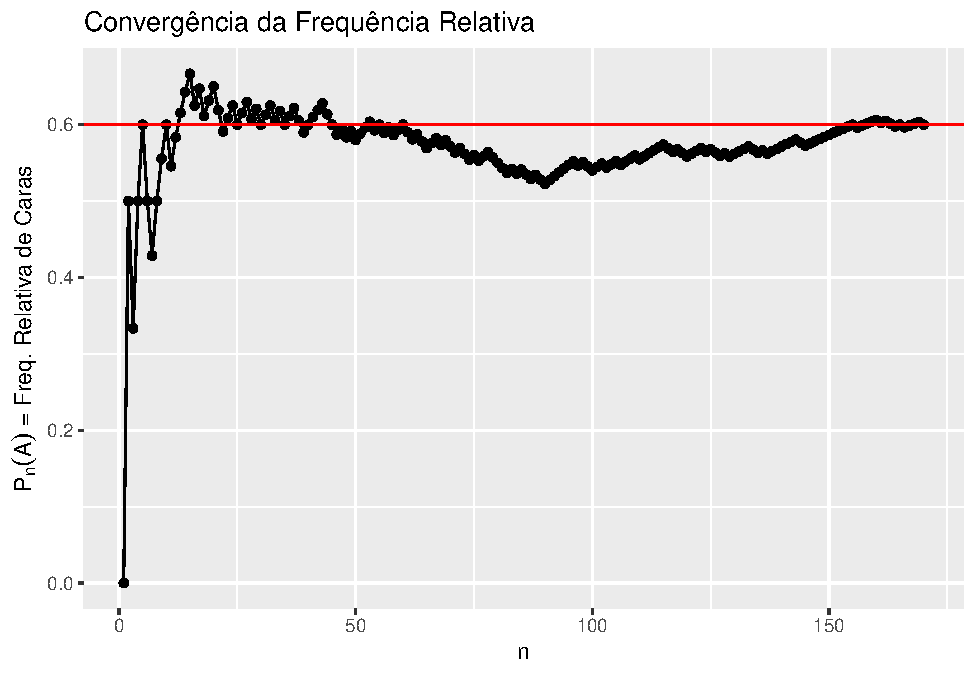
\includegraphics[width=0.8\linewidth]{InfBayes_files/figure-latex/unnamed-chunk-1-1} \end{center}

\(~\)

\begin{itemize}
\tightlist
\item
  \textbf{Interpretação Lógica} (Keynes, Jeffreys, Carnap, etc.)

  \begin{itemize}
  \tightlist
  \item
    medida de ``vínculo parcial'' entre uma evidência e uma hipótese;
  \item
    baseia-se em relações objetivas entre proposições.
  \item
    \textbf{Exemplo:} considere duas proposições: ``até agora todos os lançamentos resultaram em cara'' e ``será realizado um novo lançamento''. Pode-se afirmar que ``provavelmente o resultado do novo lançamento será cara''.
  \end{itemize}
\end{itemize}

\(~\)

\begin{itemize}
\tightlist
\item
  \textbf{Interpretação Subjetivista} (Ramsey, de Finetti, Savage, etc)

  \begin{itemize}
  \tightlist
  \item
    probabilidade como medida subjetiva de crença;
  \item
    baseada na experiência de cada indivíduo, portanto única.
  \item
    \textbf{Exemplo:} suponha que Bruno lançou uma moeda 3 vezes e todos os resultados foram cara. Esse indivíduo, em posse dessa informação, pode acreditar que o resultado cara é mais provável que coroa. Contudo, quando pergunta sobre a probabilidade de cara ao seu colega Olavo, ignorante com relação a moeda, ele responde que é 1/2.
  \end{itemize}
\end{itemize}

\(~\)

\hypertarget{relauxe7uxe3o-de-crenuxe7a-precsim}{%
\section{\texorpdfstring{Relação de Crença \(\precsim\)}{Relação de Crença \textbackslash precsim}}\label{relauxe7uxe3o-de-crenuxe7a-precsim}}

\(\precsim\) : relação de ``crença'' em \(\mathcal{A}\times\mathcal{A}\)

\begin{itemize}
\tightlist
\item
  \(A \prec B\) : acredito mais em \(B\) que em \(A\) (\(B \succ A\))
\item
  \(A \sim B\) : acredito igualmente em \(B\) e \(A\)
\item
  \(A \precsim B\) : acredito em \(B\) pelo menos tanto quanto em \(A\)
\end{itemize}

\textbf{Objetivo:} sob certas condições em \(\precsim\), obter uma medida de probabilidade \(P\) que representa (concorda) com \(\precsim\).

\[A \precsim B ~ \Longleftrightarrow ~ P(A) \leq P(B)\]

\(~\)

\textbf{Suposições sobre \(\precsim\)}

\textbf{SP1:} Para \(A, B \in \mathcal{A}\), exatamente uma das afirmações a seguir deve valer:\\
\[A \prec B ~,~ B \prec A ~\textrm{ou}~ A \sim B.\]

\(~\)

\textbf{SP2:} \(A_1, A_2, B_1, B_2 \in \mathcal{A}\) tais que \(A_1 \cap A_2 = B_1 \cap B_2 = \varnothing\) e \(A_i \precsim B_i\), \(i=1,2\). Então
\[A_1 \cup A_2 \precsim B_1 \cup B_2 .\]
Além disso, se \(A_i \prec B_i\) para algum \(i\), então \(A_1 \cup A_2 \prec B_1 \cup B_2 .\)

\(~\)

\textbf{SP3:} Se \(A\) é um evento, então \(\varnothing \precsim A\). Além disso, \(\varnothing \prec \Omega\).

\(~\)

\textbf{SP4:} Se \(A_1, A_2, \ldots\) uma sequência decrescente de eventos, isto é, \(A_n \supseteq A_{n+1}, \forall n\), e \(B\) tal que \(B \precsim A_n, \forall n\) então \[B \precsim \bigcap_{n \geq 1} A_n.\]

\(~\)

\textbf{Lema 1:} \(A, B, D \in \mathcal{A}\) tais que \(A \cap D = B \cap D = \varnothing\). Então \[A \precsim B ~\Leftrightarrow~ A \cup D \precsim B \cup D\]

\begin{quote}
\textbf{Demo:}\\
(\(\Rightarrow\)) \(A \precsim B \Rightarrow A \cup D \precsim B \cup D\) (SP2)\\
(\(\Leftarrow\)) \(B \prec A \Rightarrow B \cup D \prec A \cup D\) (SP2)
\end{quote}

\(~\)

\textbf{Teorema 1:} Se \(A \precsim B\) e \(B \precsim D\) então \(A \precsim D\).

\begin{quote}
\textbf{Demo:}
\end{quote}

\begin{center}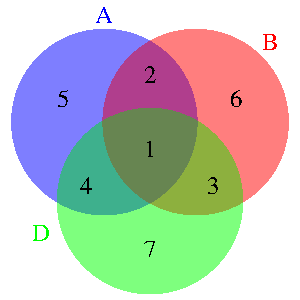
\includegraphics[width=0.8\linewidth]{InfBayes_files/figure-latex/Venn-1} \end{center}

\begin{enumerate}
\def\labelenumi{(\roman{enumi})}
\tightlist
\item
  \((1) \cup (2) \cup (4) \cup (5) \precsim (1) \cup (2) \cup (3) \cup (6)\) \(~\Rightarrow~ (4) \cup (5) \precsim (3) \cup (6)\).\\
\item
  Analogamente, \((2) \cup (6) \precsim (4) \cup (7)\)\\
  De (i) e (ii) e pelo Lema 1, \((4) \cup (5) \cup (2) \cup (6) \precsim (3) \cup (6) \cup (4) \cup (7)\)\\
  \(~\Rightarrow~ (2) \cup (5) \precsim (3) \cup (7)\) \({~\Rightarrow~ (2) \cup (5) \cup (1) \cup(4) \precsim (3) \cup (7) \cup (1) \cup(4)}\).
\end{enumerate}

\(~\)

\textbf{Teorema 2 (generalização do SP2):}
Se \(A_1, \ldots, A_n\) são eventos disjuntos e \(B_1, \ldots, B_n\) são também eventos disjuntos tais que \(A_i \precsim B_i\), para \(i=1,\ldots,n\), então \[\bigcup_{i=1}^{n} A_i \precsim \bigcup_{i=1}^{n} B_i.\]
Se \(A_i \prec B_i\) para algum i, então \(\bigcup_{i=1}^{n} A_i \prec \bigcup_{i=1}^{n} B_i.\)

\begin{quote}
\textbf{Demo:} Basta aplicar SP2 \(n-1\) vezes.
\end{quote}

\(~\)

\textbf{Teorema 3:}
Se \(A \precsim B\) então \(A^c \succsim B^c\).

\begin{quote}
\textbf{Demo:} Do Lema 1, \(A \cup (A^c \cap B^c) \precsim B \cup (A^c \cap B^c)\) \(\Rightarrow B^c \cup (A \cap B) \precsim A^c \cup (A \cap B)\) \(\Rightarrow B^c \precsim A^c\).
\end{quote}

\(~\)

\textbf{Resultado:} Para todo evento \(A\), \(A \precsim \Omega\).

\begin{quote}
\textbf{Demo:} Por SP3, \(\varnothing \precsim A^c\). Tomando \(D=A\) no Lema 1, \(\varnothing \cup A \precsim A^c \cup A \Rightarrow A \precsim \Omega\).
\end{quote}

\(~\)

\textbf{Teorema 4:}
Se \(A \subseteq B\) então \(A \precsim B\).

\begin{quote}
\textbf{Demo:} Suponha, \(B \prec A\). Tomando \(D=B^c\) no Lema 1, \(B \cup B^c \prec A \cup B^c \Rightarrow \Omega \prec A \cup B^c\). Absurdo!
\end{quote}

\(~\)

\textbf{Exemplo 1:} \(\omega_0 \in \Omega\). \(A \precsim B \Leftrightarrow \{\omega_0 \in B\) \textbf{ou} \(\omega_0 \notin (A \cup B)\}\). Mostre que \(\precsim\) obedece a SP1 a SP4.

\begin{quote}
(SP1)\\
\(A \precsim B \Leftrightarrow \omega_0 \in B \cup (A \cup B)^c\)
\(\Rightarrow B \prec A \Leftrightarrow \omega_0 \in B^c \cap (A \cup B)\)
\(\Leftrightarrow \omega_0 \in A \cap B^c.\)\\
Analogamente, \(A \prec B \Leftrightarrow \omega_0 \in B \cap A^c.\)\\
\(A \sim B \Leftrightarrow A \precsim B\) e \(B \precsim A\)
\(\Leftrightarrow \omega_0 \in [B \cup (A \cup B)^c] \cap [A \cup (A \cup B)^c]\)
\(\Leftrightarrow \omega_0 \in (A \cap B) \cup (A \cup B)^c.\)\\
\(~\)\\
(SP2)\\
\(A_i \precsim B_i , i=1,2 \Leftrightarrow\) \(\omega_0 \in [B_1 \cup (A_1 \cup B_1)^c] \cap [B_2 \cup (A_2 \cup B_2)^c]\) \(\Leftrightarrow \omega_0 \in [(B_1 \cup B_2) \cap D^c] \cup (A_1 \cup B_1 \cup A_2 \cup B_2)^c,\)\\
com \(D = (A_1 \cap B2) \cup (A_2 \cap B1).\)\\
\(A_1 \cup A_2 \precsim B_1 \cup B_2 \Leftrightarrow\) \(\omega_0 \in (B_1 \cup B_2) \cup (A_1 \cup A_2 \cup B_1 \cup B_2)^c\)\\
Como \((B_1 \cup B_2) \cap D^c \subseteq (B_1 \cup B_2)\), vale o SP2.\\
\(~\)\\
(SP3)\\
\(\varnothing \precsim A \Leftrightarrow \omega_0 \in A \cup (\varnothing \cup A)^c\) \(\Leftrightarrow \omega_0 \in A \cup A^c = \Omega.\)\\
Como \(\Omega\) é não-vazio, \(\exists \omega_0 \in \Omega\) e, portanto, \(\varnothing \prec \Omega\).\\
\(~\)\\
(SP4) Exercício!
\end{quote}

\(~\)

\textbf{Exemplo 2:} \(\Omega = \mathbb{N}\), \(\mathcal{A} = \mathcal{P}(\mathbb{N})\). \(A \precsim B \Leftrightarrow \{B\) é infinito \textbf{ou} \(A\) e \(B\) são finitos com \(|A| \leq |B|\}\). Verifique se \(\precsim\) satisfaz SP1 a SP4.

\(~\)

\textbf{Teorema 5:} Se \(A_1 \subseteq A_2 \subseteq \ldots\) é uma sequência crescente de eventos e \(B\) é tal que \(A_n \precsim B, \forall n\) então \[\bigcup_{n \geq 1} A_n \precsim B.\]

\begin{quote}
\textbf{Demo:} \(A_n^c \supseteq A_{n+1}^c\) e, pelo Teo 3, \(A_n^c \succsim B^c\), \(\forall n\).\\
Por SP4, \(\bigcap_{n \geq 1} A_n^c \succsim B^c\) \(\Rightarrow \bigcup_{n \geq 1} A_n \precsim B.\)
\end{quote}

\(~\)

\textbf{Teorema 6:} \(\left(A_n\right)_{n \geq 1}\) e \(\left(B_n\right)_{n \geq 1}\) sequências tais que \(A_i \cap A_j = B_k \cap B_l = \varnothing\), \(\forall i \neq j\), \(\forall k \neq l\).
\[A_i \precsim B_i, \forall i ~\Rightarrow~ \bigcup_{n \geq 1} A_n \precsim \bigcup_{n \geq 1} B_n.\]
Se existe ao menos um \(j\) tal que \(A_j \prec B_j\) então \(\displaystyle{ \bigcup_{n \geq 1} A_n \prec \bigcup_{n \geq 1} B_n }.\)

\begin{quote}
\textbf{Demo:} Da extensão de SP2, temos que \(\displaystyle{ \bigcup_{i = 1}^n A_i \precsim \bigcup_{i = 1}^n B_i }\), \(\forall n \geq 1\) \(~\Rightarrow~ \displaystyle{ \bigcup_{i = 1}^n A_i \precsim \bigcup_{i = 1}^{\infty} B_i }\), \(\forall n \geq 1\) \(~\Rightarrow~ \displaystyle{ \bigcup_{i = 1}^{\infty} A_i \precsim \bigcup_{i = 1}^{\infty} B_i }~\) (Teo 5)\\
\(\exists n_0\) tal que \(A_{n_0} \prec B_{n_0}\). De SP2, temos que, para \(n \geq n_0\),\\
\(\displaystyle \bigcup_{i = 1}^{n_0} A_i = \bigcup_{i = 1}^{n_0-1} A_i \cup A_{n_0} \prec \bigcup_{i = 1}^{n_0-1} B_i \cup B_{n_0} = \bigcup_{i = 1}^{n_0} B_i\) \(~\Rightarrow~ \displaystyle \bigcup_{i = 1}^{n_0} A_i \prec \bigcup_{i = 1}^{n_0} B_i.\)\\
Da primeira parte, temos que \(\displaystyle{ \bigcup_{i = n_0+1}^{\infty} A_i \precsim \bigcup_{i = n_0+1}^{\infty} B_i } ~\) e, por SP2,\\
\(\displaystyle \bigcup_{i = 1}^{n_0} A_i \cup \bigcup_{i = n_0+1}^{\infty} A_i \prec \bigcup_{i = 1}^{n_0} B_i \cup \bigcup_{i = n_0+1}^{\infty} B_i\)\\
provando o resultado.
\end{quote}

\(~\)

\hypertarget{medida-de-probabilidade-que-representa-precsim}{%
\section{\texorpdfstring{Medida de Probabilidade que ``representa'' \(\precsim\)}{Medida de Probabilidade que ``representa'' \textbackslash precsim}}\label{medida-de-probabilidade-que-representa-precsim}}

\(~\)

\textbf{SP5:} Existe uma variável aleatória \(X: \Omega \longrightarrow \mathbb{R}\), \(\mathcal{A}\)-mensurável, tal que \(X(\omega) \in [0,1], \forall \omega \in \Omega\) e, se \(I_1\) e \(I_2\) são intervalos contidos em \([0,1]\), \(\{X \in I_1\} \precsim \{X \in I_2\} \Leftrightarrow \lambda(I_1) \leq \lambda(I_2)~.\)

\begin{itemize}
\item
  Se \(I=[a,b] \subseteq [0,1]\), \(\lambda(I) = b-a\) é o comprimento do intervalo \(I\) (medida de Lebesgue).
\item
  ``Experimento auxiliar'' ; \(X \sim\) Uniforme{[}0,1{]}.
\item
  \(\{X \in [a,b]\}\) \(\sim \{X \in (a,b]\}\) \(\sim \{X \in [a,b)\}\) \(\sim \{X \in (a,b)\}\).
\end{itemize}

\(~\)

\textbf{Teorema 7:} Seja \(A \in \mathcal{A}\). Então \(\exists! a^* \in [0,1]\) tal que \(A \sim \{X \in [0,a^*]\}\).

\begin{quote}
\textbf{Demo:} Seja \(U(A) = \left\{ a \in [0,1] : A \precsim \{X \in [0,a]\} \right\}\).\\
\(1 \in U(A)\) pois \(\Omega = \{X \in [0,1]\} \succsim A\) \(~\Rightarrow~ U(A) \neq \varnothing\).\\
Tome \(a^* = \inf U(A)\).\\
\(~\)\\
(i) Considere \((a_n)_{n \geq 1}\), \(a_n \in [0,1], \forall n \geq 1\), tal que \(a_n \geq a_{n+1} \geq a^*\) e \(a_n \downarrow a^*\). Então, \(\forall n \geq 1\) , \(\{X \in [0,a_n]\} \succsim A\).\\
Por SP4, \(\displaystyle \bigcap_{n=1}^\infty \{X \in [0,a_n]\} \succsim A\) \(~\Rightarrow~ \{X \in [0,a^*]\} \succsim A\)\\
\(~\)\\
(ii) Se \(a^*=0\) , \(\{X \in [0,0]\} \sim \varnothing \precsim A\) (por SP3).\\
Se \(a^* > 0\) , considere \((a_n)_{n \geq 1}\) com \(a_n \leq a_{n+1} < a^*\) e \(a_n \uparrow a^*\).\\
\(\{X \in [0,a_n]\} \precsim A, \forall n \geq 1\) e, pelo Teo 5, \(\displaystyle \bigcup_{n=1}^{\infty} \{X \in [0,a_n]\} \precsim A\) \(~\Rightarrow~ \{X \in [0,a^*)\} \sim \{X \in [0,a^*]\} \precsim A\).\\
\(~\)\\
De (i) e (ii), temos que \(A \sim \{X \in [0,a^*]\}\).\\
\(~\)\\
\(a^*\) é único pois se \(a_1 < a^* < a_2\) são outros valores quaisquer, segue que \(\{X \in [0,a_1]\} \prec \{X \in [0,a^*]\} \prec \{X \in [0,a_2]\}\) e só um desses eventos pode ser equivalente à \(A\).
\end{quote}

\(~\)

\textbf{Teorema 8:} A probabilidade do evento \(A\), \(P(A)\), é definida como \(a^* \in [0,1]\) tal que \(A \sim \{X \in [0,a^*]\}\). Assim, \(A \sim \left\{X \in \left[0,P(A)\right]\right\}\). A função de probabilidade assim definida satisfaz:
\[A \precsim B ~\Leftrightarrow~ P(A) \leq P(B).\]

\begin{quote}
\textbf{Demo:} Do Teo 7, \(A \sim \left\{X \in \left[0,P(A)\right]\right\}\) e \(B \sim \left\{X \in \left[0,P(B)\right]\right\}\).\\
\(A \precsim B\) \(~\Leftrightarrow~ \left\{X \in \left[0,P(A)\right]\right\} \precsim \left\{X \in \left[0,P(B)\right]\right\}\) \(~\Leftrightarrow~ \lambda \left([0,P(A)]\right) \precsim \lambda \left([0,P(B)]\right)\) \(~\Leftrightarrow~ P(A) \leq P(B).\)
\end{quote}

\(~\)

\textbf{Teorema 9:} A função \(P: \mathcal{A} \longrightarrow [0,1]\) que, para cada \(A \in \mathcal{A}\), associa \(P(A)\) tal que \(A \sim \left\{X \in \left[0,P(A)\right]\right\}\) é uma medida de probabilidade (no sentido \(\sigma\)-aditiva).

\begin{quote}
\textbf{Demo:}
(i) \(P(A) \geq 0\).\\
\(\Omega \sim \{X \in [0,1]\}\Rightarrow P(\Omega)=1\).\\
\(\varnothing \sim \{X \in [0,0]\} \Rightarrow P(\varnothing)=0\)\\
\(\varnothing \precsim A \Rightarrow 0 \leq P(A)\).\\
\(~\)\\
(ii) Seja \(A\) e \(B\) tal que \(A \cap B = \varnothing\). Vamos mostrar que \(P(A \cup B) = P(A) + P(B)\).\\
Pelo Teo 8, \(A \sim \{ X \in [0,P(A)]\}\), \(B \sim \{ X \in [0,P(B)]\}\), \(A \cup B \sim \{ X \in [0,P(A \cup B)]\}\).\\
Como \(A \subseteq A \cup B\) e, por SP3, \(A \precsim A \cup B\), vale que \(P(A) \leq P(A \cup B)\). Vamos verificar que \(B \sim \left\{X \in \left(P(A),P(A \cup B) \right]\right\}\).\\
Suponha, por absurdo, \(B \prec \left\{X \in \left(P(A),P(A \cup B) \right]\right\}\).\\
\(A \precsim \{X \in [0,P(A)]\}\) \(~\overset{SP2}{\Longrightarrow}~\)
\(A \cup B \prec \{X \in [0,P(A)]\} \cup \left\{X \in \left(P(A),P(A \cup B) \right]\right\}\)
\(~\Rightarrow~ A \cup B \prec \left\{X \in [0,P(A)] \cup \left(P(A),P(A \cup B) \right]\right\}\)
\(~\Rightarrow~ A \cup B \prec \left\{X \in \left[0,P(A \cup B) \right]\right\}~\) (Absurdo!)\\
Analogamente, \(B \succ \left\{X \in \left(P(A),P(A \cup B) \right]\right\}\) é absurdo! Logo, \(B \sim \left\{X \in \left(P(A),P(A \cup B) \right]\right\} \sim \left\{X \in \left[0, P(A \cup B)-P(A) \right]\right\}\).\\
Como \(B \sim \left\{X \in \left[0,P(B)\right]\right\}\), temos que \(P(A \cup B) = P(A) + P(B)\).
\end{quote}

\(~\)

\textbf{Corolário 1:} Se \(A_1, \ldots, A_n\) são eventos disjuntos, então \(P\left(\bigcup_{i=1}^{n} A_i\right) = \sum_{i=1}^{n} P\left(A_i\right)\).

\begin{quote}
\textbf{Demo:} Basta repetir o argumento da segunda parte da demonstração anterior \(n-1\) vezes.
\end{quote}

\(~\)

\textbf{Teorema 10:} Seja \(A_1 \supseteq A_2 \supseteq \ldots\) uma seq. decrescente de eventos tais que \(\bigcap_{i=1}^{\infty} A_i = \varnothing\). Então \(\displaystyle \lim_{n \uparrow \infty} P(A_n) = 0\).

\begin{quote}
\textbf{Demo:} \(A_1 \supseteq A_2 \supseteq \ldots\) \(\Rightarrow\) \(P(A_1) \geq P(A)_2 \geq \ldots\).\\
Além disso, \(\displaystyle \lim_{n \uparrow \infty} P(A_n) = b\). Como \(P(A_n) \geq b\), \(\forall n\), segue que \(A_n \succsim \{X \in [0,b]\}\), \(\forall n\).\\
Por SP4, \(\varnothing = \bigcap_{i=n}^{\infty} A_i \succsim \{X \in [0,b]\}\).\\
Se \(b>0\), então \(\{X \in [0,b]\} \succ \{X \in [0,b/2]\} \succsim \varnothing\). Como essa relação contradiz a anterior, temos que \(b\) deve ser igual a \(0\).
\end{quote}

\(~\)

\textbf{Teorema 9: (conclusão)}
Usando o Corolário 1 e o Teorema 10 é possível concluir a demonstração do Teorema 9, mostrando que \(P\) é \(\sigma\)-aditiva, isto é, \[P\left(\bigcup_{i=1}^{\infty} A_i\right) = \sum_{i=1}^{\infty} P\left(A_i\right) ~,~~ A_i \cap A_j = \varnothing, \forall i \neq j.\]

\begin{quote}
\textbf{Demo:} Seja \((A_n)_{n \geq 1}\) sequência de eventos disjuntos. Segue do Corolário 1 que\\
(i) \(\displaystyle P\left(\bigcup_{i=1}^{\infty} A_n\right) = \sum_{i=1}^{n} P\left(A_i\right) + P\left(\bigcup_{j=n+1}^{\infty} A_j\right)\), \(n=1,2,\ldots\)\\
Considere \(\displaystyle B_n=\bigcup_{j=n+1}^{\infty} A_j\), \(n \geq 1\), uma sequência decrescente de eventos tais que \(\displaystyle \bigcap_{n=1}^{\infty} B_n = \varnothing\). Pelo Teorema 10, segue que \(\displaystyle \lim_{n\uparrow \infty} P(B_n) = 0\). Assim, tomando o limite do lado direito de (i), segue que\\
\(\displaystyle P\left(\bigcup_{i=1}^{\infty} A_i\right)\) \(=\displaystyle \lim_{n\uparrow \infty} \sum_{i=1}^{n} P\left(A_i\right) + \lim_{n\uparrow \infty} P\left(B_n\right)\) \(=\displaystyle \sum_{i=1}^{\infty} P\left(A_i\right)\).
\end{quote}

\(~\)

\textbf{Teorema 11:} Se a relação de crença \(\precsim\) obedece SP1 a SP5 então \(\exists !~ P: \mathcal{A} \rightarrow [0,1]\), medida de probabilidade, tal que \(P\) representa \(\precsim~.\)

\begin{quote}
\textbf{Demo:}
Já foi mostrado que \(P\) é uma medida de probabilidade \(\sigma\)-aditiva, de modo que apenas resta mostrar a unicidade de \(P\).\\
Considere que existe uma outra medida \(P'\) que concorde com a relação \(\precsim\). Como \(X\sim\text{Unif}(0,1)\), \(P'\left(\left\{X\in[0,a]\right\}\right)=a\). Se \(A\) é um evento, existe um único \(a^*\) tal que \(A\sim\{X\in[0,a^*]\}\) e, como \(P'\) concorda com a relação \(\precsim\),\\
\(P'(A)\) \(=P'\left(\left\{X\in[0,a^*]\right\}\right)\) \(=a^*\) \(=P(A)~.\)
\end{quote}

\(~\)

\hypertarget{medida-de-probabilidade-condicional}{%
\section{Medida de Probabilidade Condicional}\label{medida-de-probabilidade-condicional}}

\textbf{Nova Relação:} \((A|D) \precsim (B|D)\) (Sabendo que \(D\) ocorreu, \(B\) é preferível a \(A\)).

\begin{itemize}
\item
  Para \(D = \Omega\), temos o caso anterior: \(A \precsim B\) \(\Leftrightarrow (A|\Omega) \precsim (B|\Omega)\).
\item
  Suponha que vale as suposições SP1 a SP5 e, adicionalmente,
\end{itemize}

\textbf{SP6:} \((A|D) \precsim (B|D) \Leftrightarrow (A \cap D) \precsim (B \cap D)\) \(~~\Big( (A \cap D|\Omega) \precsim (B \cap D|\Omega) \Big)\)

\(~\)

\textbf{Propriedades decorrentes de SP1 a SP6:}

\begin{enumerate}
\def\labelenumi{\arabic{enumi}.}
\item
  \(\forall A,B,D\), \((A|D) \precsim (B|D)\) ou \((B|D) \precsim (A|D)\).
\item
  Se \((A|D) \precsim (B|D)\) e \((B|D) \precsim (E|D)\) então \((A|D) \precsim (E|D)\).
\item
  \(A,B,D,E\) com \(A \cap D \cap E \sim B \cap D \cap E \sim \varnothing\). \newline \((A|D) \precsim (B|D)\) \(\Leftrightarrow\) \((A \cup E|D) \precsim (B \cup E|D)\).
\item
  \((A|D) \precsim (B|D)\) \(\Leftrightarrow\) \((A^c|D) \succsim (B^c|D)\).
\item
  Seja \(B, D\) e \((A_n)_{n \geq 1}\) tal que \(A_n \supseteq A_{n+1}\).\\
  \((B|D) \precsim (A_n|D)\), \(\forall n\), então \(\displaystyle (B|D) \precsim \left(\bigcap_{n=1}^{\infty} A_n|D\right)\).
\item
  \((A_n)_{n \geq 1}\) e \((B_n)_{n \geq 1}\) tal que \(A_i \cap A_j \sim A_k \cap A_l \sim \varnothing\), \(i \neq j\), \(k \neq l\), e \((A_n|D) \precsim (B_n|D), \forall n\). Então \(\displaystyle \left(\bigcup_{n=1}^{\infty} A_n | D \right) \precsim \left(\bigcup_{n=1}^{\infty} B_n | D \right)\)
\end{enumerate}

\(~\)

\textbf{Teorema 12:} \(\forall A, B, D \in \mathcal{A}\), considere \(\precsim\) satisfazendo SP1 a SP6. Então \(P: \mathcal{A} \rightarrow [0,1]\) de modo que para cada \(A \in \mathcal{A}\) é associada \(P(A) \in [0,1]\) tal que \(A \sim \left\{X \in \left[0,P(A)\right]\right\}\) é uma medida de probabilidade que representa \(\precsim\), isto é, \[(A|\Omega) \precsim (B|\Omega) \Leftrightarrow P(A) \leq P(B).\] Além disso, se \(D \in \mathcal{A}\) é tal que \(P(D) \geq 0\), então \[(A|D) \precsim (B|D) \Leftrightarrow P(A|D) \leq P(B|D),\] onde \(P(\cdot|D): \mathcal{A} \rightarrow [0,1]\) é uma medida de probabilidade tal que
\[P(A|D) = \frac{P(A \cap D)}{P(D)}.\]

\hypertarget{Bayes}{%
\chapter{Introdução à Inferência Bayesiana}\label{Bayes}}

\hypertarget{BasBayes}{%
\section{Conceitos Básicos}\label{BasBayes}}

\begin{itemize}
\item
  \textbf{Inferência Estatística:} fazer afirmações sobre quantidades não observáveis em um determinado contexto.
\item
  \(\theta\) : \textbf{parâmetro} - quantidade desconhecida de interesse (não-observável em determinado contexto).
\item
  \(\Theta\) : \textbf{espaço paramétrico} - conjunto onde \(\theta\) toma valores (supostamente conhecido).
\item
  \(E=\left(\boldsymbol X, \theta, \left\{f(\boldsymbol x|\theta)\right\}\right)\): \textbf{experimento} - ``\emph{tornar visível algo que antes era invisível}'' ou, mais especificamente no nosso contexto, observar uma realização \(\boldsymbol x \in \mathfrak{X}\) de um vetor aleatório \(\boldsymbol X\) com alguma distribuição \(f(\boldsymbol x|\theta)\). Essa distribuição pertence, na maioria dos casos, à uma família de distribuições fixada mas que depende do parâmetro desconhecido de interesse \(\theta\). Note que na grande maioria dos problemas do dia a dia de um estatístico ele se utiliza de resultados experimentais para fazer afirmações sobre \(\theta\) e este, por sua vez, é não-observável em geral.
\item
  \(\mathfrak{X}\) : \textbf{espaço amostral} - conjunto onde \(\boldsymbol X\) toma valores (supostamente conhecido).
\item
  \(\mathcal{F}\) : \(\sigma\)-álgebra de (sub)conjuntos de \(\mathfrak{X}\).
\item
  Neste espaço amostral, defini-se uma família \(\mathcal{P}=\{P(\cdot|\theta): \theta \in \Theta\}\), isto é, um conjunto de distribuições (condicionais) para \(\boldsymbol X\) indexadas por \(\theta\).
\item
  \((\mathfrak{X},\mathcal{F},\mathcal{P})\) : modelo estatístico (clássico).
\item
  \(V_x(\theta)=f(\boldsymbol x |\theta)\) : função de verossimilhança.
\end{itemize}

\(~\)

\hypertarget{inferuxeancia-frequentista-ou-cluxe1ssica}{%
\subsection{Inferência Frequentista (ou Clássica)}\label{inferuxeancia-frequentista-ou-cluxe1ssica}}

\begin{itemize}
\item
  \(\theta\) é considerado fixo (apesar de desconhecido) e, portanto, não recebe uma distribuição de probabilidade.
\item
  Baseia-se no " princípio" da amostragem repetida (interpretação frequentista de probabilidade), isto é, supõe que é possivel realizar infinitas vezes o experimento. Assim, o \(\boldsymbol x\) é apenas um dos possiveis resultados (hipóteticos) do experimento.
\item
  Probabilidade somente é definida em (uma \(\sigma\)-álgebra de) \(\mathfrak{X}\).
\end{itemize}

\hypertarget{inferuxeancia-bayesiana}{%
\subsection{Inferência Bayesiana}\label{inferuxeancia-bayesiana}}

\begin{itemize}
\item
  Baseia-se na interpretação subjetivista de probabilidade, de modo que a \emph{SUA} incerteza sobre algo desconhecido deve ser quantificada (traduzida) em termos de probabilidade.
\item
  Assim, \emph{SUA} incerteza sobre o parâmetro (desconhecido) é representada por uma distribuição de probabilidade, \(\theta\) é tratado como uma variável aleatória (v.a.) e \emph{SUA} distribuição para \(\theta\) antes da realização do experimento, \(f(\theta),\) é chamada de \textbf{distribuição a priori}. Note que a atribuição de uma distribuição a prior para \(\theta\) independe da natureza do parâmetro, ele pode ser a proporção de indivíduos que avalia positivamente o governo atual (quantidade essa que muda a todo instante) ou ainda a milésima casa do \(\pi\) (algum número de 0 a 9, fixo porém desconhecido no momento dessa leitura).
\item
  A atualização de \emph{SUA} incerteza sobre \(\theta,\) incorporando uma nova informação trazida pelos dados \(\boldsymbol x\) (representada por \(f(\boldsymbol x| \theta)\)) é feita pelo \emph{Teorema de Bayes}:
\item
  \textbf{Teorema de Bayes:}
\end{itemize}

\[\underbrace{f(\theta| \boldsymbol x)}_{dist. posteriori}=~~\dfrac{f(\theta)f(\boldsymbol x|\theta)}{\displaystyle \int_{\Theta}f(\boldsymbol x|\theta)dP_\theta} ~\propto~ \underbrace{f(\theta)}_{priori}\overbrace{f(\boldsymbol x|\theta)}^{verossimilhança}.\]

\begin{itemize}
\tightlist
\item
  Toda a inferência sobre \(\theta\) será baseada exclusivamente em \(f(\theta| \boldsymbol x)\), não sendo necessário considerar pontos amostrais que poderiam mas não foram observados (como é feito na inferência frequentista).
\end{itemize}

\(~\)

\begin{itemize}
\tightlist
\item
  \textbf{Observação:} será utilizada a notação geral para integral (de Lebesgue):
\end{itemize}

\[\displaystyle \int_{\Theta}f(\boldsymbol x|\theta)dP_\theta
= \left\{ \begin{array}{ll} \displaystyle \int_{\Theta}f(\boldsymbol x|\theta) f(\theta) d\theta ~&~ \text{(caso abs. contínuo)}\\ \displaystyle \sum_{\Theta}f(\boldsymbol x|\theta) f(\theta) ~&~ \text{(caso discreto)} \end{array}\right.\]

\(~\)

\textbf{Exemplo 1a.} Suponha que existem duas moedas, uma delas tem \(\theta =1/2\) (honesta) e a outra \(\theta=3/4\) (viesada). Uma moeda é escolhida e é feito um lançamento da moeda selecionada. Nesse experimento, tem-se \(X|\theta \sim Ber(\theta)\), com \(\Theta=\{1/2,3/4\}\) e \(\mathfrak{X}=\{0,1\}\). Como ``chutar'' o valor de \(\theta\)?

Considere que não existe razão para você acreditar que há algum tipo de preferência na escolha de uma ou outra moeda, isto é, considere que a priori \(f(\theta=1/2)\) \(=f(\theta=3/4)\) \(=1/2\). Suponha que o lançamento resultou em cara (\(x=1\)). Então

\(f(\theta = 3/4|X=1)\) \(=\dfrac{f(X=1|\theta=3/4)f(\theta=3/4)}{\sum_\theta f(X=1|\theta)f(\theta)}\) \(=\dfrac{\dfrac{3}{4}\dfrac{1}{2}}{\dfrac{3}{4}~\dfrac{1}{2}+\dfrac{1}{2}~\dfrac{1}{2}}=\) \(\dfrac{3/4}{5/4}=\dfrac{3}{5}\) \(= 1-\underbrace{f(\theta=1/2|X=1)}_{2/5}\).

Se, no entando, o resultado do lançamento da moeda fosse coroa (\(x=0\)), teríamos

\(P(\theta=3/4|X=0)\) \(=\dfrac{\dfrac{1}{4}~\dfrac{1}{2}}{\dfrac{1}{4}~\dfrac{1}{2}+\dfrac{1}{2}~\dfrac{1}{2}}\) \(=\dfrac{1/2}{1/2+2/2}=\dfrac{1}{3}\).

\begin{center}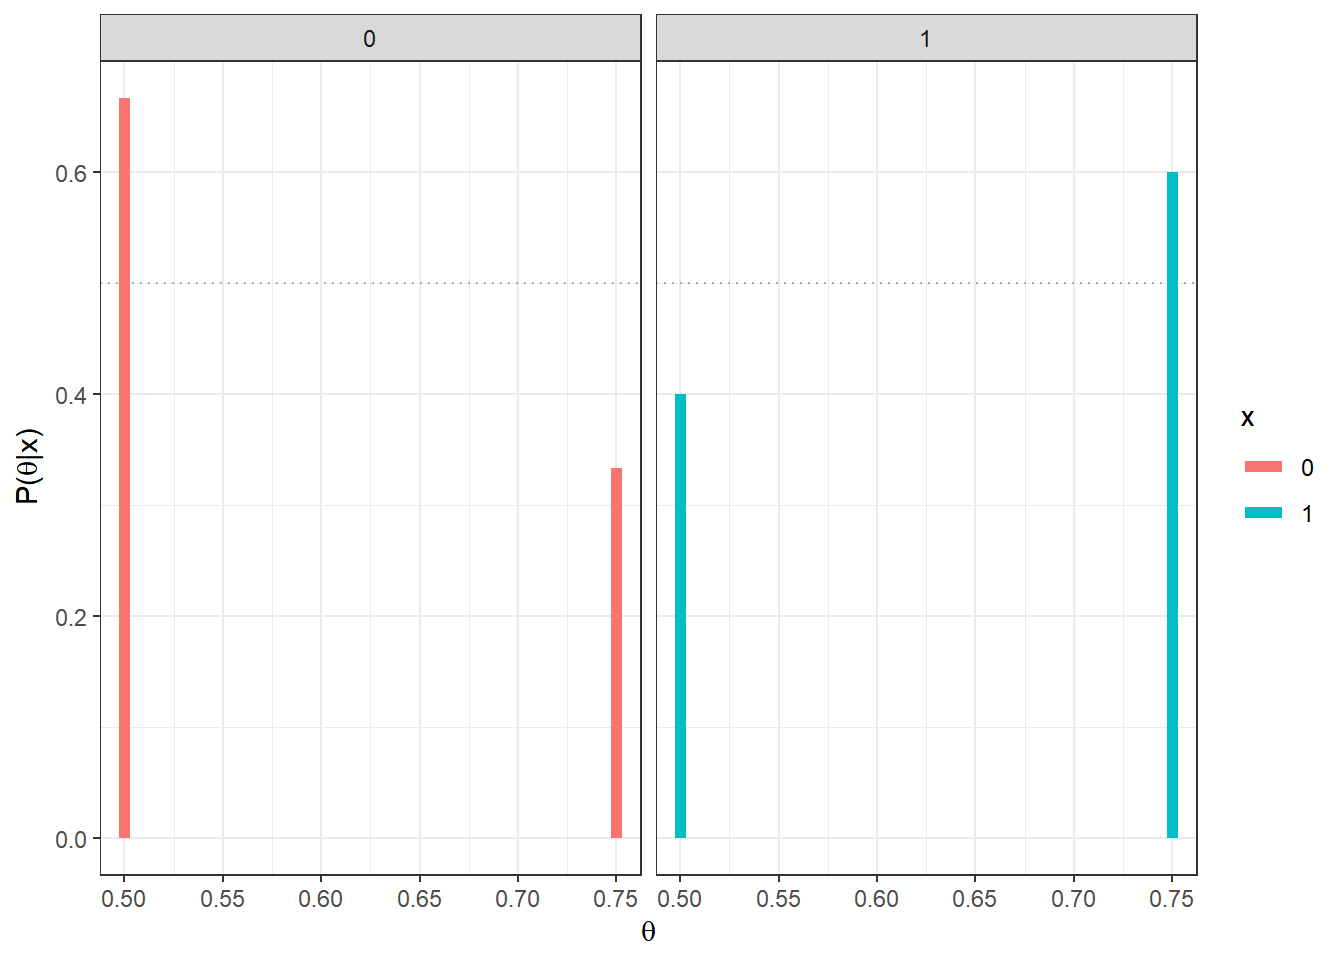
\includegraphics[width=0.8\linewidth]{InfBayes_files/figure-latex/unnamed-chunk-2-1} \end{center}

Assim, se sua decisão for escolher o valor mais provável de \(\theta\) após observar \(x\), a conclusão seria que a moeda é viesada \((\theta=3/4)\) se for observado cara \((x=1)\) e que a moeda é honesta \((\theta=1/2)\) se o resultado for coroa \((x=0)\).

\(~\)

\textbf{Exemplo 1b.} Considere agora que serão realizados \(n\) lançamentos da moeda, de modo que agora tem-se \(X|\theta \sim Bin(n,\theta)\), \(\theta \in \{1/2,3/4\}\), \(x \in \{0,1,\ldots,n\}\). Suponha que observa-se \(X=x\).

\(f(\theta=3/4|X=x)\) \(=\dfrac{f(x|\theta=3/4)f(\theta=3/4)}{\displaystyle \sum_{\theta\in \{1/2,3/4\}}f(x|\theta)f(\theta)}\) \(=\dfrac{\displaystyle \binom{n}{x}\left(\dfrac{3}{4}\right)^x\left(\dfrac{1}{4}\right)^{n-x}\dfrac{1}{2}}{\displaystyle \binom{n}{x}\left(\dfrac{3}{4}\right)^x\left(\dfrac{1}{4}\right)^{n-x}\dfrac{1}{2}+\displaystyle\binom{n}{x}\left(\dfrac{1}{2}\right)^x\left(\dfrac{1}{2}\right)^{n-x}\dfrac{1}{2}}\) \(=\dfrac{1}{1+\left(\dfrac{2^n}{3^x}\right)}\) \(=\dfrac{3^x}{3^x + 2^n}\).

\begin{Shaded}
\begin{Highlighting}[]
\NormalTok{theta =}\StringTok{ }\KeywordTok{c}\NormalTok{(}\FloatTok{0.5}\NormalTok{,}\FloatTok{0.75}\NormalTok{)}
\NormalTok{prior=}\FloatTok{0.5} \CommentTok{# priori P(theta[1]) = 1-P(theta[2])}
\NormalTok{n=}\DecValTok{5}\NormalTok{;}
\NormalTok{post =}\StringTok{ }\ControlFlowTok{function}\NormalTok{(x)\{ }
\NormalTok{  (prior}\OperatorTok{*}\KeywordTok{dbinom}\NormalTok{(x,n,theta)) }\OperatorTok{/}\StringTok{ }\KeywordTok{sum}\NormalTok{(prior }\OperatorTok{*}\StringTok{ }\KeywordTok{dbinom}\NormalTok{(x,n,theta)) \}}
\KeywordTok{tibble}\NormalTok{(}\DataTypeTok{x=}\KeywordTok{as.factor}\NormalTok{(}\KeywordTok{rep}\NormalTok{(}\KeywordTok{seq}\NormalTok{(}\DecValTok{0}\NormalTok{,n),}\DataTypeTok{each=}\KeywordTok{length}\NormalTok{(theta))),}
    \DataTypeTok{x1=}\KeywordTok{rep}\NormalTok{(theta,(n}\OperatorTok{+}\DecValTok{1}\NormalTok{)),}\DataTypeTok{x2=}\KeywordTok{rep}\NormalTok{(theta,(n}\OperatorTok{+}\DecValTok{1}\NormalTok{)),}\DataTypeTok{y1=}\DecValTok{0}\NormalTok{,}
    \DataTypeTok{y2=}\KeywordTok{as.vector}\NormalTok{(}\KeywordTok{apply}\NormalTok{(}\KeywordTok{matrix}\NormalTok{(}\KeywordTok{seq}\NormalTok{(}\DecValTok{0}\NormalTok{,n)),}\DecValTok{1}\NormalTok{,post))) }\OperatorTok\StringTok{ }
\StringTok{  }\KeywordTok{ggplot}\NormalTok{() }\OperatorTok{+}\StringTok{ }\KeywordTok{geom_hline}\NormalTok{(}\DataTypeTok{yintercept=}\FloatTok{0.5}\NormalTok{, }\DataTypeTok{col=}\StringTok{"darkgrey"}\NormalTok{,}\DataTypeTok{lty=}\DecValTok{3}\NormalTok{) }\OperatorTok{+}
\StringTok{  }\KeywordTok{geom_segment}\NormalTok{(}\KeywordTok{aes}\NormalTok{(}\DataTypeTok{x=}\NormalTok{x1,}\DataTypeTok{xend=}\NormalTok{x2,}\DataTypeTok{y=}\NormalTok{y1,}\DataTypeTok{yend=}\NormalTok{y2,}\DataTypeTok{colour=}\NormalTok{x),}\DataTypeTok{lwd=}\DecValTok{2}\NormalTok{) }\OperatorTok{+}\StringTok{ }
\StringTok{  }\KeywordTok{xlab}\NormalTok{(}\KeywordTok{expression}\NormalTok{(theta)) }\OperatorTok{+}\StringTok{ }\KeywordTok{ylab}\NormalTok{(}\KeywordTok{expression}\NormalTok{(}\KeywordTok{paste}\NormalTok{(}\StringTok{"P("}\NormalTok{,theta,}\StringTok{"|x)"}\NormalTok{))) }\OperatorTok{+}
\StringTok{  }\KeywordTok{theme_bw}\NormalTok{()}\OperatorTok{+}
\StringTok{  }\KeywordTok{facet_wrap}\NormalTok{(}\OperatorTok{~}\NormalTok{x)}
\end{Highlighting}
\end{Shaded}

\begin{center}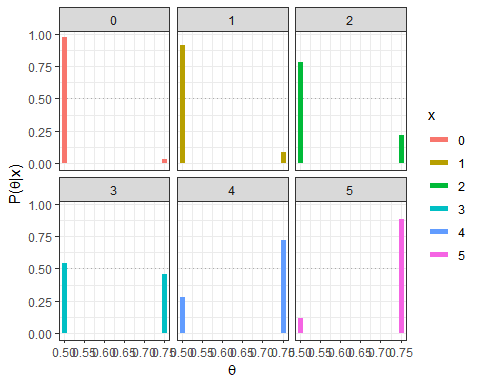
\includegraphics[width=0.8\linewidth]{InfBayes_files/figure-latex/unnamed-chunk-4-1} \end{center}

\(~\)

Note que o Exemplo 1.a é um caso particular desse exemplo com \(n=1\). Se novamente sua decisão é baseada no valor mais provável de \(\theta\), deve-se escolher \(\theta=3/4\) se

\(f(\theta=3/4|X=x) > f(\theta=1/2|X=x)\) \(\Longleftrightarrow f(\theta=3/4|X=x) > \dfrac{1}{2}\) \(\Longleftrightarrow \dfrac{3^x}{3^x + 2^n} > \dfrac{1}{2}\) \(\Longleftrightarrow {3^x} > {2^n}\) \(\Longleftrightarrow \dfrac{x}{n} = \bar{x} > \log_3{2}\approx 0,63\).

\(~\)

\textbf{Exemplo 1c.} Considere que uma moeda será lançada \(n\) vezes mas que \(\theta\) é desconhecido, de modo que \(\Theta = [0,1]\). Para simplificar, vamos assumir \(f(\theta)=\mathbb{I}_{[0,1]}(\theta)\), isto é, \(\theta \sim Unif(0,1)\sim Beta(1,1)\). Essa priori corresponde ao caso em que você acredita que todos os valores possíveis para \(\theta\) são igualmente ``prováveis'', assim como nos exemplos anteriores. Novamente, \(X|\theta \sim Bin(n,\theta)\)

\(f(\theta|x)\)
\(=\dfrac{f(x|\theta)f(\theta)}{\displaystyle\int_0^1 f(x|\theta)f(\theta)d\theta}\)
\(=\dfrac{\displaystyle\binom{n}{x}~\theta^x(1-\theta)^{n-x} ~~\mathbb{I}_{[0,1]}(\theta)}{\displaystyle\int_0^1\binom{n}{x}~\theta^x(1-\theta)^{n-x}d\theta}=\) \(\dfrac{\tfrac{\Gamma(1+x+1+n-x)}{\Gamma(1+x)\Gamma(1+n-x)}~~\theta^x(1-\theta)^{n-x}~~\mathbb{I}_{[0,1]}(\theta)}{\underbrace{\displaystyle \int_0^1\tfrac{\Gamma(1+x+1+n-x)}{\Gamma(1+x)\Gamma(1+n-x)}~~\theta^x(1-\theta)^{n-x}d\theta}_{1}}\)
\(=\tfrac{\Gamma(1+x+1+n-x)}{\Gamma(1+x)\Gamma(1+n-x)}~~\theta^x(1-\theta)^{n-x}~~\mathbb{I}_{[0,1]}(\theta)\).

Logo \(\theta|x \sim Beta(1+x,1+n-x)\). Nesse exemplo, o valor ``mais provável'' (com maior densidade a posteriori) para \(\theta\) é a moda da distribuição, \(Moda(\theta|x)\) \(= \dfrac{(1+x)-1}{(1+x)+(1+n-x)-2}\) \(= \dfrac{x}{n}\) \(=\bar{x}\). Suponha que foi observado \(n=5\) e \(x=2\), a posteriori é \(\theta|x=2 \sim Beta(3,4)\) e a moda é \(Moda(\theta|x)\) \(=\frac{1+x-1}{1+1+n-2}\) \(=\frac{2}{5}\) \(=0,4\);

\begin{center}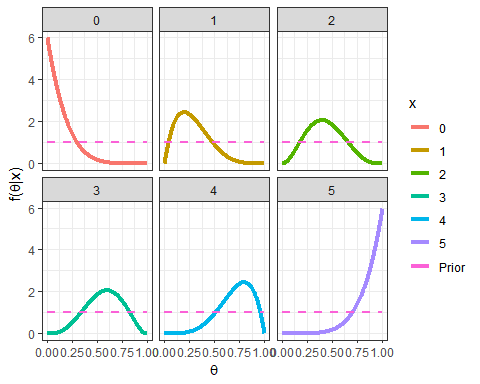
\includegraphics[width=0.8\linewidth]{InfBayes_files/figure-latex/unnamed-chunk-6-1} \end{center}

Algumas medidas resumo da distribuição posterior para esse exemplo são

\begin{itemize}
\item
  \(Moda(\theta|x)\) \(=\dfrac{1+x-1}{1+1+n-2}\) \(=\dfrac{2}{5}\) \(=0,4\);
\item
  \(E[\theta|x]\) \(=\dfrac{1+x}{1+1+n}\) \(=\dfrac{3}{7}\) \(=0,43\);
\item
  \(Med(\theta|x)\) \(\approx \dfrac{1+x-1/3}{1+1+n-2/3}\) \(=\dfrac{8/3}{19/3}\) \(\approx 0,42\);
\item
  \(Var(\theta|x)\) \(=\dfrac{(1+x)(1+n-x)}{(1+1+n)^2(1+1+n+1)}\) \(=\dfrac{12}{392}\) \(\approx 0,031\).
\end{itemize}

\(~\)

\textbf{Exemplo 1d.} Por fim, suponha que no exemplo anterior, sua opinião a priori é representada por uma distribuição beta qualquer com parâmetros \(a\) e \(b\), \(a,b > 0\). Desta forma, \(X|\theta \sim Bin(n,\theta)\) e \(\theta\sim Beta(a,b)\). Calculando a distribuição a posteriori de forma similar ao exemplo anterior, temos que \(\theta|X=x \sim Beta(a+x,b+n-x)\). Note que o exemplo anterior é o caso particular em que \(a=b=1~.\)

\(~\)

\begin{Shaded}
\begin{Highlighting}[]
\NormalTok{theta =}\StringTok{ }\KeywordTok{seq}\NormalTok{(}\DecValTok{0}\NormalTok{,}\DecValTok{1}\NormalTok{,}\FloatTok{0.01}\NormalTok{)}
\NormalTok{a=}\DecValTok{2}\NormalTok{; b=}\DecValTok{2}\NormalTok{;}
\NormalTok{n=}\DecValTok{5}
\NormalTok{vero1 =}\StringTok{ }\KeywordTok{as.vector}\NormalTok{(}\KeywordTok{apply}\NormalTok{(}\KeywordTok{matrix}\NormalTok{(}\KeywordTok{seq}\NormalTok{(}\DecValTok{0}\NormalTok{,n)),}\DecValTok{1}\NormalTok{,}
            \ControlFlowTok{function}\NormalTok{(x)\{}\KeywordTok{dbeta}\NormalTok{(theta,}\DecValTok{1}\OperatorTok{+}\NormalTok{x,}\DecValTok{1}\OperatorTok{+}\NormalTok{n}\OperatorTok{-}\NormalTok{x)\}))}
\NormalTok{post1 =}\StringTok{ }\KeywordTok{as.vector}\NormalTok{(}\KeywordTok{apply}\NormalTok{(}\KeywordTok{matrix}\NormalTok{(}\KeywordTok{seq}\NormalTok{(}\DecValTok{0}\NormalTok{,n)),}\DecValTok{1}\NormalTok{,}
            \ControlFlowTok{function}\NormalTok{(x)\{}\KeywordTok{dbeta}\NormalTok{(theta,a}\OperatorTok{+}\NormalTok{x,b}\OperatorTok{+}\NormalTok{n}\OperatorTok{-}\NormalTok{x)\}))}
\KeywordTok{tibble}\NormalTok{(}\DataTypeTok{x=}\KeywordTok{as.factor}\NormalTok{(}\KeywordTok{rep}\NormalTok{(}\KeywordTok{seq}\NormalTok{(}\DecValTok{0}\NormalTok{,n),}\DataTypeTok{each=}\KeywordTok{length}\NormalTok{(theta))),}
    \DataTypeTok{theta=}\KeywordTok{rep}\NormalTok{(theta,(n}\OperatorTok{+}\DecValTok{1}\NormalTok{)),}\DataTypeTok{post=}\NormalTok{post1,}\DataTypeTok{vero=}\NormalTok{vero1) }\OperatorTok\StringTok{ }
\StringTok{  }\KeywordTok{ggplot}\NormalTok{() }\OperatorTok{+}\StringTok{ }
\StringTok{  }\KeywordTok{geom_line}\NormalTok{(}\KeywordTok{aes}\NormalTok{(}\DataTypeTok{x=}\NormalTok{theta,}\DataTypeTok{y=}\KeywordTok{dbeta}\NormalTok{(theta,a,b),}\DataTypeTok{linetype=}\StringTok{"Prior"}\NormalTok{,}\DataTypeTok{colour=}\StringTok{"Prior"}\NormalTok{),}\DataTypeTok{lwd=}\DecValTok{1}\NormalTok{) }\OperatorTok{+}
\StringTok{  }\KeywordTok{geom_line}\NormalTok{(}\KeywordTok{aes}\NormalTok{(}\DataTypeTok{x=}\NormalTok{theta,}\DataTypeTok{y=}\NormalTok{post,}\DataTypeTok{linetype=}\StringTok{"Posterior"}\NormalTok{,}\DataTypeTok{colour=}\NormalTok{x),}\DataTypeTok{lwd=}\FloatTok{1.3}\NormalTok{) }\OperatorTok{+}
\StringTok{  }\KeywordTok{geom_line}\NormalTok{(}\KeywordTok{aes}\NormalTok{(}\DataTypeTok{x=}\NormalTok{theta,}\DataTypeTok{y=}\NormalTok{vero,}\DataTypeTok{linetype=}\StringTok{"Verossimilhança"}\NormalTok{,}\DataTypeTok{colour=}\NormalTok{x),}\DataTypeTok{lwd=}\DecValTok{1}\NormalTok{) }\OperatorTok{+}\StringTok{ }
\StringTok{  }\KeywordTok{xlab}\NormalTok{(}\KeywordTok{expression}\NormalTok{(theta)) }\OperatorTok{+}\StringTok{ }\KeywordTok{ylab}\NormalTok{(}\KeywordTok{expression}\NormalTok{(}\KeywordTok{paste}\NormalTok{(}\StringTok{"f("}\NormalTok{,theta,}\StringTok{"|x)"}\NormalTok{))) }\OperatorTok{+}
\StringTok{  }\KeywordTok{theme_bw}\NormalTok{()}\OperatorTok{+}\KeywordTok{labs}\NormalTok{(}\DataTypeTok{linetype=}\StringTok{""}\NormalTok{)}\OperatorTok{+}
\StringTok{  }\KeywordTok{facet_wrap}\NormalTok{(}\OperatorTok{~}\NormalTok{x)}
\end{Highlighting}
\end{Shaded}

\begin{center}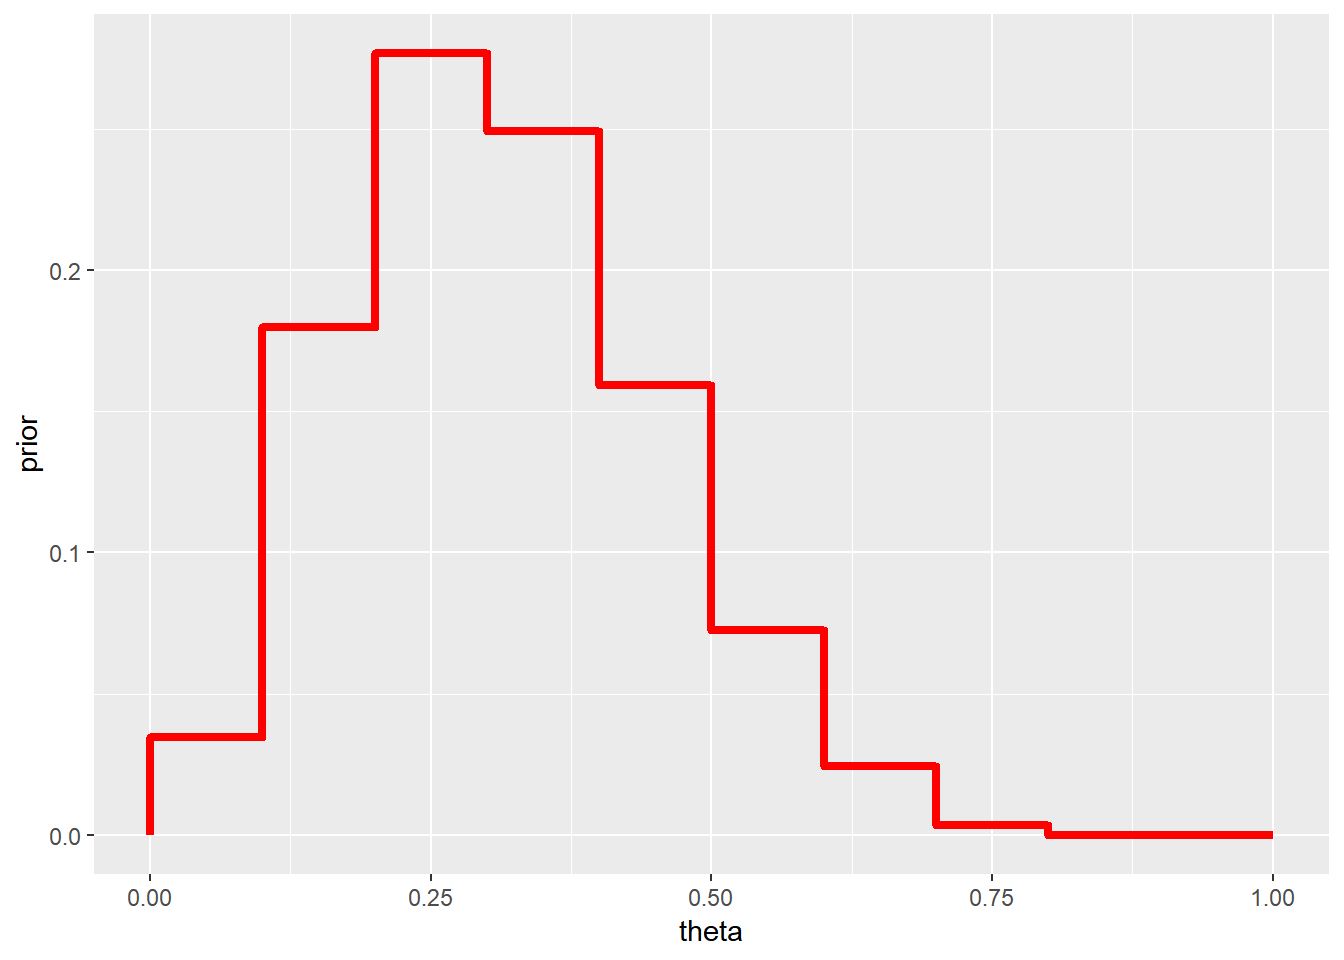
\includegraphics[width=0.8\linewidth]{InfBayes_files/figure-latex/unnamed-chunk-8-1} \end{center}

\(~\)

Suponha agora que \(a=b=2\), \(n=5\) e \(x=2\), de modo que \(\theta|x=2 \sim Beta(4,5)\). Algumas medidas resumo da distribuição posterior para esse exemplo são

\begin{itemize}
\item
  \(Moda(\theta|x)\) \(=\dfrac{a+x-1}{a+b+n-2}\) \(=\dfrac{3}{7}\) \(\approx 0,428\);
\item
  \(E[\theta|x]\) \(=\dfrac{a+x}{a+b+n}\) \(=\dfrac{4}{9}\) \(\approx 0,444\);
\item
  \(Med(\theta|x)\) \(\approx \dfrac{a+x-1/3}{a+b+n-2/3}\) \(=\dfrac{11/3}{25/3}\) \(\approx 0,440\);
\item
  \(Var(\theta|x)\) \(=\dfrac{(a+x)(b+n-x)}{(a+b+n)^2(a+b+n+1)}\) \(=\dfrac{20}{810}\) \(\approx 0,0247\).
\end{itemize}

\(~\)

\(~\)

\hypertarget{teorema-de-de-finetti}{%
\section{Teorema de De Finetti}\label{teorema-de-de-finetti}}

\textbf{Definição.} Uma coleção finita \(X_1,X_2,\ldots,X_n\) de quantidades aleatórias é dita \emph{permutável} se a distribuição de \(\left(X_{\pi_1},\ldots,X_{\pi_n}\right)\) é a mesma para toda permutação \(\boldsymbol\pi=(\pi_1,\ldots,\pi_n)\) dos índices \((1,\ldots,n)\). Uma coleção infinita de quantidades aleatórias é \emph{permutável} se toda subcoleção é permutável.

\(~\)

\begin{itemize}
\tightlist
\item
  Segue da definição que cada uma das variáveis \(X_1,\ldots,X_n\) tem a mesma distribuição marginal. Além disso, \((X_i,X_j)\) têm mesma distribuição que \((X_k,X_l)\), \(\forall i\neq j\) e \(k\neq l\), e assim por diante.
\end{itemize}

\(~\)

\textbf{Proposição.} Uma coleção \(C\) de variáveis aleatórias é permitável se, e somente se, para todo \(n\) finito menor ou igual ao tamanho da coleção \(C\), toda \(n\)-upla (sequência ordenada de \(n\) elementos) de elementos distintos de \(C\) têm a mesma distribuição que toda outra \(n\)-upla.

\(~\)

\begin{quote}
\textbf{Exemplo 1.} Considere uma coleção \(X_1,X_2,\ldots\) uma sequência (finita ou infinita) de variáveis aleatórias independentes e identicamente distribuidas (v.a. i.i.d). Note que \(f(x_1,\ldots,x_n)=\displaystyle\prod_{i=1}^nf(x_i)~,\) \(\forall n~,\) de modo que \(\left(X_{i_1},\ldots,X_{i_n}\right)\) têm a mesma distribuição de \(\left(X_{j_1},\ldots,X_{j_n}\right)\), para \(i_1\neq\ldots\neq i_n\) e \(j_1\neq\ldots\neq j_n\). Então, toda coleção de v.a. i.i.d é permutável.
\end{quote}

\(~\)

\begin{quote}
\textbf{Exemplo 2:} Foi visto no exemplo anterior que a suposição que uma sequência de v.a. é i.i.d. implica que tal sequência é também permutável. Sabe-se também que independência implica em correlação nula, \(\rho=0\). Será então que v.a. identicamente distribuídas e não correlacionadas são também permutáveis?\\
\(~\)
\end{quote}

\begin{tabular}{ccccc}
\toprule
$X_1~$ / $~X_2$ & $-1$ & $0$ & $+1$ & $f(x_1)$\\
\midrule
$-1$ & $0.10$ & $0.05$ & $0.15$ & $0.3$\\
$0$ & $0.15$ & $0.20$ & $0.05$ & $0.4$\\
$+1$ & $0.05$ & $0.15$ & $0.10$ & $0.3$\\
$f(x_2)$ & $0.3$ & $0.4$ & $0.3$ & $1.0$\\
\bottomrule
\end{tabular}

\(~\)\\
\(cor(X_1,X_2)\)
\(=\frac{\text{Cov}\left(X_1,X_2\right)}{\sqrt{\text{Var}(X_1)\text{Var}(X_2)}}\)
\(=\frac{\text{E}\left[\left(X_1-\text{E}[X_1]\right)\left(X_2-\text{E}[X_2]\right)\right]}{\sqrt{\text{Var}(X_1)\text{Var}(X_2)}}\)
\(=\frac{\text{E}\left[X_1X_2\right]-\text{E}[X_1]\text{E}[X_2]}{\sqrt{\text{Var}(X_1)\text{Var}(X_2)}}\)\\
\(E(X_1)=E(X_2)=0\)\\
\(E(X_1X_2)=-1\cdot0,2+0+1\cdot0,2=0\) \(\Rightarrow cor(X_1,X_2)=0\)\\
\((X_1,X_2)\) são identicamente distribuídas e não correlacionadas mas não são permutáveis pois, por exemplo, \(P\big((X_1,X_2)=(1,-1)\big)~\neq~P\big((X_2,X_1)=(1,-1)\big)~.\)

\(~\)

\begin{quote}
\textbf{Exemplo 3:} Suponha que \(X_1,X_2,\ldots\) são condicionalmente i.i.d. dado \(Y=y\) com densidade \(f(x_i|y),\;i=1,2,\ldots\) e \(Y\) tem densidade \(h(y)\). Então \(X_1,X_2,\ldots\) são permutaveis.\\
\(f_{X_{i_1},\ldots,X_{i_n}}(x_1,\ldots,x_n)\) \(=\displaystyle\int\prod_{j=1}^nf(x_j|y)h(y)dy,\) para qualquer \(n\)-upla \(X_{i_1},\ldots,X_{i_n}\). Note que o lado direito não depende dos rótulos \(i_1,\ldots,i_n\).
\end{quote}

\(~\)

\(~\)

\textbf{Teorema de Representação de De Finetti.} (para v.a. Bernoulli)

Uma sequência infinita \(\left(X_n\right)_{n\geq 1}\) de v.a. Bernoulli é permutável se, e somente se, existe uma v.a \(\theta\) em \([0,1]\) tal que, condicional a \(\theta\), \(\left(X_i\right)_{n\geq 1}\) são i.i.d. \(Ber(\theta)\). Além disso, se a sequência é permutável, então a distribuição de \(\theta\) é única e \(\displaystyle\dfrac{1}{n}\sum_{i=1}^\infty X_i \underset{n\uparrow\infty}{\overset{q.c.}{\longrightarrow}}\theta~.\)

\(P(X_1=x_1,\ldots,X_n=x_n)\) \(=\displaystyle\int_0^1\theta^{\sum x_i}(1-\theta)^{n-\sum x_i}~dF(\theta)\) \(=\displaystyle\int_0^1\prod_{i=1}^n\underbrace{\theta^{x_i}(1-\theta)^{1-x_i}}_{f(x_i|\theta)}~f(\theta)~d\theta\)

\(F(\theta)=\displaystyle\lim_{n\uparrow\infty}~\text{P}\left(\dfrac{\sum_iX_i}{n}\leq \theta\right)~.\)

\(~\)

\(~\)

\begin{quote}
\textbf{Exemplo 4:} (1.19/1.20 - Schervish)\\
Seja \(\left(X_n\right)_{n\geq 1}\) v.a. Bernoulli.\\
\(~\)\\
Considere que o \emph{Estatístico 1} acredita que \(P_1(X_1=x_1,\ldots,X_n=x_n)\) \(=\dfrac{12}{x+2}\dfrac{1}{\binom{n+4}{x+2}}~,\) de modo que \(P_1(X_1=1)\) \(=\dfrac{12}{3}\dfrac{3!~2!}{5!}\) \(=\dfrac{4}{10}\) \(=0,4~.\)\\
Por outro lado, o \emph{Estatístico 2} acredita que \(P_2(X_1=x_1,\ldots,X_n=x_n)\) \(=\dfrac{1}{(n+1)\binom{n}{x}}\) e, então, \(P_2(X_1=1)=\dfrac{1}{2}=0,5~.\)\\
\(~\)\\
Contudo, pelo Teorema de Finetti, ambos acreditam que o limite \(\theta=\displaystyle\lim_{n\uparrow\infty}\frac{1}{n}\sum_{i=1}^nX_i\) existe com probabilidade 1 e que \(P(X_1=1|\theta)=\theta\), mas não tem opiniões diferentes sobre \(\theta\).\\
\(~\)\\
Suponha agora que foi observado \(\boldsymbol{x}=(x_1,\ldots,x_{20})\) com \(\displaystyle\sum_{i=1}^{20}x_i=14\). Então,\\
\(P_i(X_{21}=1|X_1=x_1,\ldots,X_{20}=x_{20})\) \(=\dfrac{P_i(X_1=x_1,\ldots,X_{20}=x_{20},X_{21}=1)}{P_i(X_1=x_1,\ldots,X_{20}=x_{20})}\)\\
de modo que,\\
\(P_1(X_{21}=1|\mathbf X=\mathbf x)=\) \(\dfrac{\dfrac{12}{17}\dfrac{1}{\binom{25}{17}}}{\dfrac{12}{16}\dfrac{1}{\binom{24}{16}}}\) \(=\dfrac{16}{17}\dfrac{\dfrac{24!}{16!8!}}{\dfrac{25!}{17!8!}}\) \(=\dfrac{16}{17}\dfrac{17}{25}\) \(=\dfrac{16}{25}=0,64\)\\
\(P_2(X_{21}=1|\mathbf X=\mathbf x)\) \(=\dfrac{\dfrac{1}{22\binom{21}{15}}}{\dfrac{1}{21\binom{20}{14}}}\) \(=\dfrac{21}{22}\dfrac{\dfrac{20!}{14!6!}}{\dfrac{21\cdot20!}{15\cdot 14!6!}}\) \(=\dfrac{21}{22}\dfrac{15}{21}\) \(=\dfrac{15}{22}=0,68\)
\end{quote}

\(~\)

\(~\)

\textbf{Teorema de Representação de De Finetti}

Uma sequência de v.a.s \(\{X_n\}_{n\geq 1}\) assumindo valores (em um subconjunto de) \(\mathbb R^K\) é permutável se, e somente se, existe uma medida de probabilidade sobre (uma \(\sigma\)-álgebra do) conjunto de funções de distribuições que ``sorteia'' uma \(F\) e, dada esta \(F\), \(\{X_n\}_{n\geq 1}\) é i.i.d. com distribuição \(F\). Isto é,

\(F_{\mathbf X}(x_1,\ldots,x_n)=\int\prod_{i=1}^n F(x_i)d\mu(F)\), \(\forall n\).

Alem disso, \(F_n\underset{n\uparrow\infty}{\longrightarrow}F^*\) e a distribuição de \(F^*=\underset{n\uparrow\infty}{lim}F_n\) é única e é \(\mu\).

\(~\)

\(~\)

\hypertarget{suficiuxeancia}{%
\section{Suficiência}\label{suficiuxeancia}}

Muitas vezes, a quantidade de dados é muito grande e desejamos ``resumir'' a informação trazida pelos dados. Uma forma de fazê-lo sem perder informação sobre o parâmetro de interesse é usar uma \emph{estatística suficiente}.

\(~\)

\textbf{Definição.} Dizemos que uma função da amostra \(T:\mathfrak{X} \rightarrow \mathbb{R}^p\) é uma \emph{estatística suficiente} (do ponto de vista \emph{frequentista}) se \(f\left(\boldsymbol x | T(\boldsymbol x),\theta\right) = f\left(\boldsymbol x | T(\boldsymbol x)\right)\).

\(~\)

Em palavras, conhecendo o valor da estatística suficiente, a distribuição da amostra (do v.a. \(\boldsymbol X\)) não depende mais do parâmetro \(\theta\). Isso quer dizer que a informação disponível na amostra \(\boldsymbol X\) sobre \(\theta\) está contida em \(T(\boldsymbol X)\). Obter uma estatística suficiente nem sempre é uma tarefa fácil mas o resultado a seguir, conhecido como \emph{critério da fatoração} permite identificar estatísticas suficientes.

\(~\)

\textbf{Teorema.} A estatística \(T:\mathfrak{X} \rightarrow \mathbb{R}^p\) é suficiente para a família de distribuições \(\left\{f(\cdot|\theta):\theta \in \Theta\right\}\) se, e somente se, para todo \(x \in \mathfrak{X}\) e para todo \(\theta \in \Theta\), podemos escrever \(f\left(\boldsymbol x | \theta\right)\) \(= u(\boldsymbol x) v\left(T(\boldsymbol x),\theta\right)\), onde \(u\) é uma função positiva que não depende de \(\theta\) e \(v\) é uma função não-negativa e depende de \(\boldsymbol x\) somente através de \(T(\boldsymbol x)\).

\(~\)

\begin{quote}
\textbf{Exemplo.} Seja \(X_1,\ldots,X_n\) v.a. tais que, condicional ao conhecimento de \(\theta\), são c.i.i.d. com \(X_1|\theta \sim Exp(\theta)\). Então,\\
\(f(\boldsymbol x|\theta)\) \(=\prod f(x_i|\theta)\) \(=\prod \theta e^{-\theta x_i} ~\mathbb{I}_{\mathbb{R+}}(x_i)\) \(=\theta^n e^{-\theta \sum x_i} ~\prod ~\mathbb{I}_{\mathbb{R+}}(x_i)\) \(= v\left(\sum x_i, \theta\right) u(\boldsymbol x)\).\\
Portanto, \(T(\boldsymbol x) = \sum x_i\) é estatística suficiente para \(\theta\). De fato, como \(T(\boldsymbol X)\) \(= \sum X_i | \theta\) \(\sim Gama(n,\theta)\) e \(\left\{X_1=x_1,\ldots,X_n=x_n\right\}\) \(\subseteq \left\{T(\boldsymbol X) = \sum X_i = \sum x_i = t\right\}~,\)\\
\(f\left(\boldsymbol x| T(\boldsymbol x),\theta\right)\) \(=\dfrac{f\left(\boldsymbol{x},T(\boldsymbol{x})|\theta\right)}{f\left(T(\boldsymbol{x})|\theta\right)}\) \(=\dfrac{f\left(\boldsymbol{x}|\theta\right)}{f\left(t|\theta\right)}\) \(=\dfrac{\theta^n e^{\theta \sum x_i} ~\prod ~\mathbb{I}_{\mathbb{R+}}(x_i)}{\frac{\theta^n}{\Gamma(n)}t^{n-1} e^{\theta t} ~\prod ~\mathbb{I}_{\mathbb{R+}}(x_i)}\) \(= \dfrac{\Gamma(n)}{t^{n-1}} ~\mathbb{I}_{\mathbb{R}_+}\left(t\right)~,\)\\
que não depende de \(\theta\).
\end{quote}

\(~\)

Sob o enfoque bayesiano, a definição de suficiência é um pouco mais intuitiva que a frequentista.

\textbf{Definição:} Dizemos que uma função da amostra \(T:\mathfrak{X} \rightarrow \mathbb{R}^p\) é uma \emph{estatística suficiente} (no sentido \emph{bayesiano}) se \(f\left(\theta | T(\boldsymbol x)\right) = f\left(\theta | \boldsymbol x\right)\), para todo \(x \in \mathfrak{X}\).

\(~\)

\begin{quote}
\textbf{Voltando ao exemplo}, suponha agora que, a priori, \(\theta \sim Gama(a,b)\). Então,\\
\(f(\theta| \boldsymbol x)\) \(\propto f(\boldsymbol x|\theta)f(\theta)\) \(\propto \theta^n e^{-\theta \sum x_i} ~~\theta^{a-1}e^{-b\theta}\) \(\propto \theta^{a+n-1} e^{-(b+\sum x_i)\theta}\)\\
Seja \(T = T(\boldsymbol X) = \sum X_i\), temos que \(T|\theta\sim Gamma(n,\theta)\), de modo que\\
\(f\left(\theta| T(\boldsymbol x)=t\right)\) \(\propto f(t|\theta)f(\theta)\) \(\propto \theta^n t^{n-1} e^{\theta t} ~~\theta^{a-1}e^{-b\theta}\) \(\propto \theta^{a+n-1} e^{-(b+t)\theta}\) , com \(t=\sum x_i\).\\
Assim, \(\theta|\boldsymbol x\) \(\sim \theta|T(\boldsymbol x)\) \(\sim Gamma\left(a+n,b+\sum x_i\right)\) e, portanto, \(T(\boldsymbol X) = \sum X_i\) é estatística suficiente para \(\theta\).
\end{quote}

\(~\)

Pelo teorema da fatoração, temos que \(f\left(\boldsymbol x | \theta\right)\) \(= u(\boldsymbol x) v\left(T(\boldsymbol x),\theta\right)\) e, portanto \(f(\theta|\boldsymbol x)\) \(\propto f(\theta) f\left(\boldsymbol x | \theta\right)\) \(\propto f(\theta) v\left(T(\boldsymbol x),\theta\right)~,\) que só depende de \(\boldsymbol x\) por meio de \(T(\boldsymbol x)\). Para os casos mais comuns, as definições são equivalentes \citep{Schervish12}.

\(~\)

Um dos princípios de inferência estatística é o \emph{princípio da suficiência}. Segundo este, se \(T\) é uma estatística suficiente para \(\theta\) e se dois pontos amostrais \(\boldsymbol x, \boldsymbol y \in \mathfrak{X}\) são tais que \(T(\boldsymbol x)=T(\boldsymbol y)\) então as inferências baseadas nesses pontos devem ser as mesmas. Adiante, retomaremos esse princípio de forma mais formal.

\(~\)

\hypertarget{distribuiuxe7uxe3o-a-priori}{%
\section{Distribuição a Priori}\label{distribuiuxe7uxe3o-a-priori}}

\begin{itemize}
\tightlist
\item
  A priori é sempre subjetiva (assim como a escolha do modelo estatístico)!

  \begin{itemize}
  \tightlist
  \item
    Por exemplo, dizer que os dados seguem uma distribuição normal, é uma escolha subjetiva, muitas vezes baseadas nas facilidades matemáticas que essa distribuição proporciona.\\
  \item
    Do mesmo modo, suponha que dois indivíduos que consideram que a distribuição do parêmetro é simétrica, com mesmas suposições sobre média e variância. O primeiro pode optar por representar sua distribuição usando uma distribuição Normal, enquanto o segundo pode utilizar uma distribuição T ou Cauchy.\\
  \end{itemize}
\item
  Não existe ``opinião errada'', existem opiniões diferentes, dado o nível de conhecimento e as experiências prévias do indivíduo. Contudo, algumas ``boas práticas'' devem ser consideradas como, por exemplo, tomar cuidado para não atribuir probabilidade nula a pontos ``possíveis'' do espaço paramétrico.\\
\item
  A priori deve ser sua opinião apenas sobre o parâmetro \(\theta\) e não deve depender de fatores como o desenho do experimento ou o objetivo do estudo.
\end{itemize}

\hypertarget{muxe9todo-do-histograma}{%
\subsection{Método do Histograma}\label{muxe9todo-do-histograma}}

\begin{itemize}
\item
  Muitas vezes, para ``extrair'' o conhecimento de um especialista, podemos dividir o espaço paramétrico em regiões e pedir para o especialista ``ordenar'' esses conjuntos, utilizando ``pesos'' que refletem a crença que o parâmetro esteja em cada uma daquelas regiões.
\item
  \textbf{Exemplo 1.} (\citet{Albert09}, pág 27)

  \begin{itemize}
  \tightlist
  \item
    Seja \(\theta\) uma proporção desconhecida \((\Theta=[0,1])\);\\
  \item
    Considere a partição \(T = \left\{[0,0.1), [0.1,0.2), \ldots, [0.9,1] \right\}\);
  \item
    Suponha que um especialistas atribui pesos \(p=(1, 5.2, 8, 7.2, 4.6, 2.1, 0.7, 0.1, 0, 0)\) a esse intervalos;\\
  \item
    A piori, nesse caso, é o histograma apresentado a seguir.
  \end{itemize}
\end{itemize}

\begin{Shaded}
\begin{Highlighting}[]
\NormalTok{p=}\KeywordTok{c}\NormalTok{(}\DecValTok{1}\NormalTok{, }\FloatTok{5.2}\NormalTok{, }\DecValTok{8}\NormalTok{, }\FloatTok{7.2}\NormalTok{, }\FloatTok{4.6}\NormalTok{, }\FloatTok{2.1}\NormalTok{, }\FloatTok{0.7}\NormalTok{, }\FloatTok{0.1}\NormalTok{, }\DecValTok{0}\NormalTok{, }\DecValTok{0}\NormalTok{)}
\NormalTok{prior =}\StringTok{ }\KeywordTok{c}\NormalTok{(}\DecValTok{0}\NormalTok{,p}\OperatorTok{/}\NormalTok{(}\KeywordTok{sum}\NormalTok{(p)))}
\KeywordTok{tibble}\NormalTok{(}\DataTypeTok{theta=}\KeywordTok{seq}\NormalTok{(}\DecValTok{0}\NormalTok{,}\DecValTok{1}\NormalTok{,}\FloatTok{0.1}\NormalTok{), prior) }\OperatorTok\StringTok{ }
\StringTok{  }\KeywordTok{ggplot}\NormalTok{(}\DataTypeTok{data=}\NormalTok{.) }\OperatorTok{+}
\StringTok{  }\KeywordTok{geom_step}\NormalTok{(}\KeywordTok{aes}\NormalTok{(}\DataTypeTok{x=}\NormalTok{theta,}\DataTypeTok{y=}\NormalTok{prior),}\DataTypeTok{direction=}\StringTok{"vh"}\NormalTok{,}\DataTypeTok{color=}\StringTok{"red"}\NormalTok{,}\DataTypeTok{lwd=}\FloatTok{1.5}\NormalTok{)}
\end{Highlighting}
\end{Shaded}

\begin{center}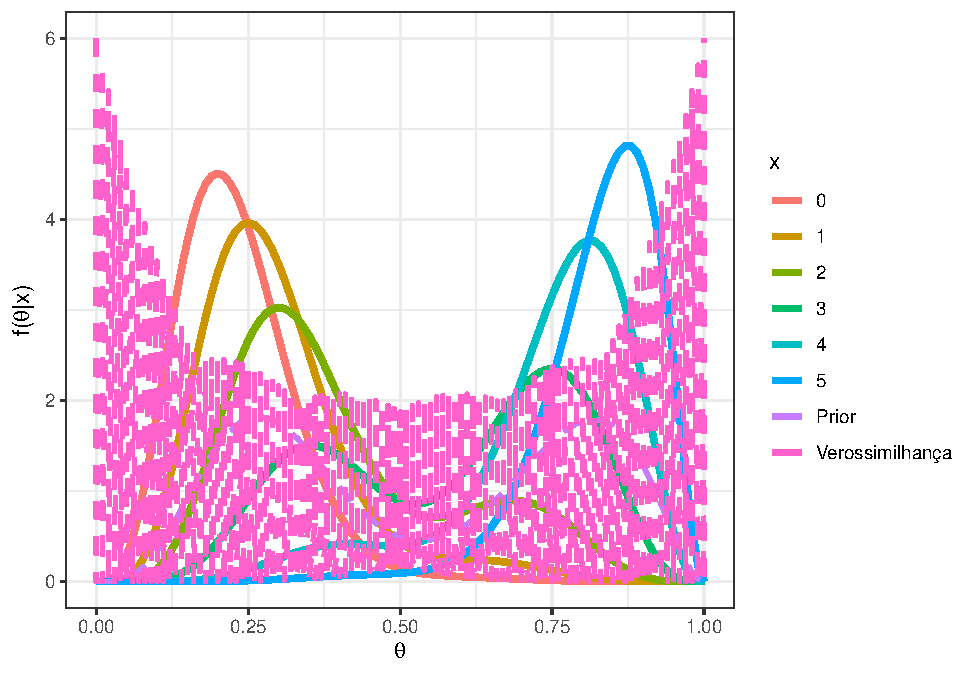
\includegraphics[width=0.8\linewidth]{InfBayes_files/figure-latex/unnamed-chunk-11-1} \end{center}

\begin{itemize}
\tightlist
\item
  Voltando ao exemplo da moeda, suponha novamente que foram observados \(x=2\) sucessos em \(n=5\) lançamentos. A posteriori nesse caso pode ser obtida multiplicando a distribuição a priori pela verossimilhança e ``padronizando'' a função obtida. Assim:
\end{itemize}

\begin{Shaded}
\begin{Highlighting}[]
\NormalTok{n=}\DecValTok{5}
\NormalTok{x=}\DecValTok{2}
\NormalTok{p =}\StringTok{ }\KeywordTok{c}\NormalTok{(}\DecValTok{1}\NormalTok{, }\FloatTok{5.2}\NormalTok{, }\DecValTok{8}\NormalTok{, }\FloatTok{7.2}\NormalTok{, }\FloatTok{4.6}\NormalTok{, }\FloatTok{2.1}\NormalTok{, }\FloatTok{0.7}\NormalTok{, }\FloatTok{0.1}\NormalTok{, }\DecValTok{0}\NormalTok{, }\DecValTok{0}\NormalTok{)}
\NormalTok{p =}\StringTok{ }\NormalTok{p}\OperatorTok{/}\NormalTok{(}\KeywordTok{sum}\NormalTok{(p))}
\NormalTok{theta =}\StringTok{ }\KeywordTok{seq}\NormalTok{(}\DecValTok{0}\NormalTok{,}\DecValTok{1}\NormalTok{,}\FloatTok{0.01}\NormalTok{)}
\NormalTok{prior =}\StringTok{ }\KeywordTok{c}\NormalTok{(}\KeywordTok{rep}\NormalTok{(p,}\DataTypeTok{each=}\DecValTok{10}\NormalTok{),}\DecValTok{0}\NormalTok{)}\OperatorTok{/}\KeywordTok{sum}\NormalTok{(}\KeywordTok{c}\NormalTok{(}\KeywordTok{rep}\NormalTok{(p,}\DataTypeTok{each=}\DecValTok{10}\NormalTok{),}\DecValTok{0}\NormalTok{))}
\NormalTok{vero =}\StringTok{ }\KeywordTok{dbinom}\NormalTok{(x,n,theta)}\OperatorTok{/}\KeywordTok{sum}\NormalTok{(}\KeywordTok{dbinom}\NormalTok{(x,n,theta))}
\NormalTok{post =}\StringTok{ }\NormalTok{(prior }\OperatorTok{*}\StringTok{ }\NormalTok{vero)}\OperatorTok{/}\KeywordTok{sum}\NormalTok{(prior }\OperatorTok{*}\StringTok{ }\NormalTok{vero)}
\NormalTok{pH =}\StringTok{ }\KeywordTok{tibble}\NormalTok{(}\DataTypeTok{theta=}\KeywordTok{rep}\NormalTok{(theta,}\DecValTok{3}\NormalTok{),}\DataTypeTok{dens=}\KeywordTok{c}\NormalTok{(prior,vero,post),}\DataTypeTok{Dist=}\KeywordTok{rep}\NormalTok{(}\KeywordTok{c}\NormalTok{(}\StringTok{'1.priori'}\NormalTok{,}\StringTok{'2.verossimilhança'}\NormalTok{,}\StringTok{'3.posteriori'}\NormalTok{),}\DataTypeTok{each=}\DecValTok{101}\NormalTok{)) }\OperatorTok\StringTok{ }
\StringTok{  }\KeywordTok{ggplot}\NormalTok{(}\DataTypeTok{data=}\NormalTok{.) }\OperatorTok{+}
\StringTok{  }\KeywordTok{geom_line}\NormalTok{(}\KeywordTok{aes}\NormalTok{(}\DataTypeTok{x=}\NormalTok{theta,}\DataTypeTok{y=}\NormalTok{dens,}\DataTypeTok{colour=}\NormalTok{Dist),}\DataTypeTok{lwd=}\FloatTok{1.5}\NormalTok{)}
\NormalTok{pH}
\end{Highlighting}
\end{Shaded}

\begin{center}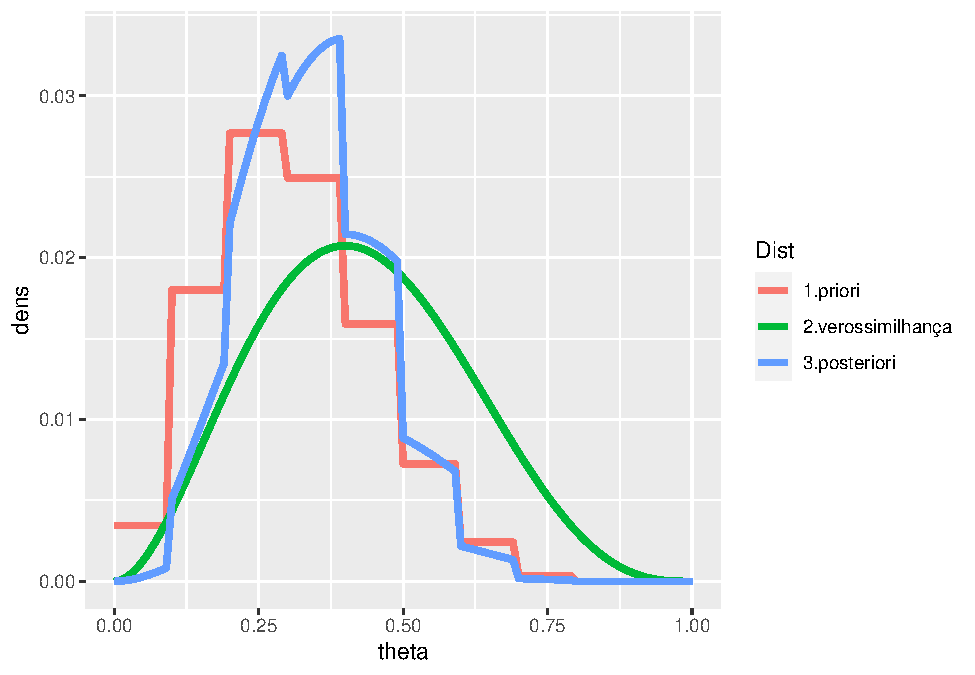
\includegraphics[width=0.8\linewidth]{InfBayes_files/figure-latex/unnamed-chunk-12-1} \end{center}

\(~\)

\hypertarget{elicitauxe7uxe3o-de-hiperparuxe2metros}{%
\subsection{Elicitação de Hiperparâmetros}\label{elicitauxe7uxe3o-de-hiperparuxe2metros}}

\begin{itemize}
\tightlist
\item
  Nessa abordagem, a priori é obtida da seguinte maneira:

  \begin{enumerate}
  \def\labelenumi{\arabic{enumi}.}
  \tightlist
  \item
    Escolha uma família de distribuições conveniente. O conceito de ``conveniência'' aqui pode levar em conta, por exemplo, o suporte da distribuição, se é flexível o suficiente para acomodar diversos tipos de opinião, se permite a obtenção analítica da posteriori e assim por diante;\\
  \item
    Obtenha um conjunto de medidas resumo (como média, variância, quantis, etc.);\\
  \item
    Utilize as medidas resumo para calcular hiperparâmetros da distribuição escolhida.
  \end{enumerate}
\end{itemize}

\(~\)

\begin{itemize}
\item
  \textbf{Exemplo:} Na seção anterior, a priori dada pelo histograma tem média \(m=0.31\) e variância aproximadamente \(v=0.02\). Podemos utilizar como priori, por exemplo, uma distribuição beta com essa média e variância, já que a beta tem um suporte conveniente e facilita as contas, como também já vimos. Assim, vamos considerar uma distribuição \(Beta(a,b)\) e escolher \(a\) e \(b\) satisfazendo:

  \begin{enumerate}
  \def\labelenumi{(\roman{enumi})}
  \tightlist
  \item
    \(E[\theta]\) \(=\dfrac{a}{a+b}\) \(=m\) \(\Longleftrightarrow b=\left(\dfrac{1-m}{m}\right)a\)
  \item
    \(Var(\theta)\) \(=\dfrac{ab}{(a+b)^2(a+b+1)}\) \(=0.02\) \(\Longleftrightarrow a=\dfrac{m(m-m^2-v)}{v}\)
  \end{enumerate}
\end{itemize}

Resolvendo o sistema temos, de forma geral, que \(a=\dfrac{m(m-m^2-v)}{v}\) e \(b=\dfrac{(1-m)(m-m^2-v)}{v}\).

Assim, no nosso exemplo, teríamos uma \(Beta(3,6.7)\). Além disso, já vimos que, nesse caso, a distribuição a posteriori é \(Beta(3+x,6.7+n-x)\). Considerando novamente \(n=5\) e \(x=2\), temos:

\begin{Shaded}
\begin{Highlighting}[]
\NormalTok{n=}\DecValTok{5}\NormalTok{; x=}\DecValTok{2}
\NormalTok{m=}\FloatTok{0.31}\NormalTok{; v=}\FloatTok{0.02}
\NormalTok{a=m}\OperatorTok{*}\NormalTok{(m}\OperatorTok{-}\NormalTok{m}\OperatorTok{^}\DecValTok{2}\OperatorTok{-}\NormalTok{v)}\OperatorTok{/}\NormalTok{v; b=(}\DecValTok{1}\OperatorTok{-}\NormalTok{m)}\OperatorTok{*}\NormalTok{(m}\OperatorTok{-}\NormalTok{m}\OperatorTok{^}\DecValTok{2}\OperatorTok{-}\NormalTok{v)}\OperatorTok{/}\NormalTok{v}
\NormalTok{p =}\StringTok{ }\KeywordTok{c}\NormalTok{(}\DecValTok{1}\NormalTok{, }\FloatTok{5.2}\NormalTok{, }\DecValTok{8}\NormalTok{, }\FloatTok{7.2}\NormalTok{, }\FloatTok{4.6}\NormalTok{, }\FloatTok{2.1}\NormalTok{, }\FloatTok{0.7}\NormalTok{, }\FloatTok{0.1}\NormalTok{, }\DecValTok{0}\NormalTok{, }\DecValTok{0}\NormalTok{)}
\NormalTok{p =}\StringTok{ }\NormalTok{p}\OperatorTok{/}\NormalTok{(}\KeywordTok{sum}\NormalTok{(p))}
\NormalTok{theta =}\StringTok{ }\KeywordTok{seq}\NormalTok{(}\DecValTok{0}\NormalTok{,}\DecValTok{1}\NormalTok{,}\FloatTok{0.01}\NormalTok{)}
\NormalTok{prior =}\StringTok{ }\KeywordTok{dbeta}\NormalTok{(theta,a,b)}\OperatorTok{/}\KeywordTok{sum}\NormalTok{(}\KeywordTok{dbeta}\NormalTok{(theta,a,b))}
\NormalTok{vero =}\StringTok{ }\KeywordTok{dbinom}\NormalTok{(x,n,theta)}\OperatorTok{/}\KeywordTok{sum}\NormalTok{(}\KeywordTok{dbinom}\NormalTok{(x,n,theta))}
\NormalTok{post =}\StringTok{ }\KeywordTok{dbeta}\NormalTok{(theta,a}\OperatorTok{+}\NormalTok{x,b}\OperatorTok{+}\NormalTok{n}\OperatorTok{-}\NormalTok{x)}\OperatorTok{/}\KeywordTok{sum}\NormalTok{(}\KeywordTok{dbeta}\NormalTok{(theta,a}\OperatorTok{+}\NormalTok{x,b}\OperatorTok{+}\NormalTok{n}\OperatorTok{-}\NormalTok{x))}
\NormalTok{priorH =}\StringTok{ }\KeywordTok{c}\NormalTok{(}\KeywordTok{rep}\NormalTok{(p,}\DataTypeTok{each=}\DecValTok{10}\NormalTok{),}\DecValTok{0}\NormalTok{)}\OperatorTok{/}\KeywordTok{sum}\NormalTok{(}\KeywordTok{c}\NormalTok{(}\KeywordTok{rep}\NormalTok{(p,}\DataTypeTok{each=}\DecValTok{10}\NormalTok{),}\DecValTok{0}\NormalTok{))}
\KeywordTok{tibble}\NormalTok{(}\DataTypeTok{theta=}\KeywordTok{rep}\NormalTok{(theta,}\DecValTok{4}\NormalTok{),}\DataTypeTok{dens=}\KeywordTok{c}\NormalTok{(prior,vero,post,priorH),}
    \DataTypeTok{Dist=}\KeywordTok{rep}\NormalTok{(}\KeywordTok{c}\NormalTok{(}\StringTok{'1.Priori Beta'}\NormalTok{,}\StringTok{'2.Verossimilhança'}\NormalTok{,}\StringTok{'3.Posteriori'}\NormalTok{,}\StringTok{'0.Priori Histograma'}\NormalTok{),}\DataTypeTok{each=}\DecValTok{101}\NormalTok{)) }\OperatorTok\StringTok{ }
\StringTok{  }\KeywordTok{ggplot}\NormalTok{(}\DataTypeTok{data=}\NormalTok{.) }\OperatorTok{+}
\StringTok{  }\KeywordTok{geom_line}\NormalTok{(}\KeywordTok{aes}\NormalTok{(}\DataTypeTok{x=}\NormalTok{theta,}\DataTypeTok{y=}\NormalTok{dens,}\DataTypeTok{colour=}\NormalTok{Dist),}\DataTypeTok{lwd=}\FloatTok{1.5}\NormalTok{)}
\end{Highlighting}
\end{Shaded}

\begin{center}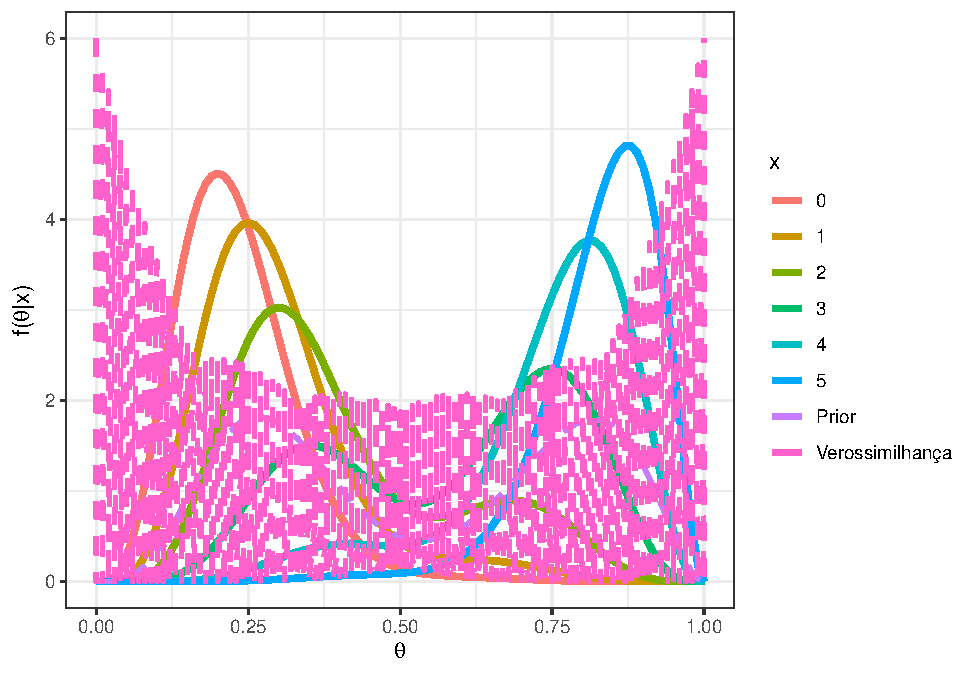
\includegraphics[width=0.8\linewidth]{InfBayes_files/figure-latex/unnamed-chunk-13-1} \end{center}

\(~\)

\hypertarget{prioris-conjugadas}{%
\subsection{Prioris Conjugadas}\label{prioris-conjugadas}}

Como visto no exemplo da moeda, em que a distribuição a priori era \(Beta(a,b)\), a posteriori era facilmente obtida e também estava na classe das distribuições \(Beta\). Em particular, quando observa-se \(x\) sucessos em \(n\) realizações de ensaios de Bernoulli, a distribuição a posteriori é \(Beta(a+x,b+n-x)\). Isso ocorre pois essa distribuição pertence à uma classe bastante espefícica de distribuições a priori, chamadas distribuições conjugadas.

\(~\)

\textbf{Definição} Seja \(\mathcal{P}=\{f(x|\theta):\;\theta \in \Theta\}\) uma família de distribuições (condicionais) para \(\boldsymbol{X}\) e considere \(\mathcal{C}=\{h(\theta|a):\;a\in A\}\) uma família de distribuições para \(\theta\). Dizemos que (a família) \(\mathcal{C}\) é \textbf{conjugada} para \(\mathcal{P}\) se, \(\forall \;h(\theta)\in \mathcal{C},\) \(h(\theta|\boldsymbol{x})\propto f(\boldsymbol x|\theta)h(\theta) \in \mathcal{C},\forall \boldsymbol x \in \mathfrak{X}.\)

\(~\)

\textbf{Resultado 1.} Seja \(X\) v.a. tal que, condicional ao conhecimento de \(\theta,\) \(X|\theta \sim Bin(n,\theta).\) Considere que, a priori, \(\theta \sim Beta(a,b).\) Então, \(\theta|X=x \sim Beta(a+x,b+n-x).\) Portanto, a família \(\mathcal{C}=\{Beta(a_1,a_2):\;(a_1,a_2)\in \mathbb{R}^2_+\}\) é conjugada para \(\mathcal{P}=\{Bin(n,\theta):\;\theta \in [0,1]\}.\)

\(~\)

\begin{itemize}
\tightlist
\item
  Esse resultado também vale se

  \begin{enumerate}
  \def\labelenumi{\arabic{enumi}.}
  \tightlist
  \item
    \(X_1,\ldots,X_n\) são v.a.s \emph{condicionalmente independentes e identicamente distribuidas} (c.i.i.d.) com \(X_i|\theta \sim Ber(\theta)\)\\
  \item
    \(X_i|\theta\sim Geo(\theta),\) \(i=1,\ldots,n \; c.i.i.d.\)\\
  \item
    \(X_i|\theta \sim BinNeg(k,\theta)\)\\
    \(\theta\sim Beta(a,b)\Rightarrow\) \(\theta|\boldsymbol X=\boldsymbol x \sim Beta(a+s,b+f)\) em que \(s\) é o número de sucessos e \(f\) é o número de fracassos.
  \end{enumerate}
\end{itemize}

\(~\)

\textbf{Resultado 2.} (\emph{generalização do resultado anterior para o caso em que o número de categorias é maior que 2})

Seja \(\boldsymbol X | \boldsymbol \theta \sim Multinomial(n,\boldsymbol \theta)\), isto é, sua função de probabilidade é dada por

\[f(\boldsymbol x| \boldsymbol \theta)= \binom{n}{x_1,x_2,\ldots,x_k}~\prod_{i=1}^{k-1}\theta^i~\underbrace{\left(1-\sum_{i=1}^{k-1}\theta_i\right)^{\displaystyle n-\sum_{i=1}^{k-1}x_i}}_{\displaystyle \theta_k^{~~x_k}}\]

em que \(\theta_i\in [0,1]\) com \(\sum_{i=1}^K\theta_i=1\), \(x_i \in \{0,1,\ldots,n\}\) com \(\sum_{i=1}^nx_i=n\) e \(\displaystyle \binom{n}{x_1,x_2,\ldots,x_k}=\dfrac{n!}{x_1!x_2!\ldots x_k!}\).

Considere que, a priori, \(\boldsymbol \theta \sim Dirichlet(a_1,\ldots,a_k),\) \(a_i > 0, i=1,\ldots,k\), isto é, a f.d.p. a priori para \(\boldsymbol \theta\) é dada por

\[f(\boldsymbol \theta) = \dfrac{\Gamma(\sum_{i=1}^K a_i)}{\Gamma(a_1)\Gamma(a_2)\ldots\Gamma(a_k)}\prod_{i=1}^{k-1}\theta_i^{a_i-1}\bigg(\underbrace{1-\sum_{i=1}^{k-1}\theta_i}_{\theta_k}\bigg)^{a_k-1}.\]

Então, a distribuição a posteriori para \(\boldsymbol \theta\) é
\(\boldsymbol \theta|\boldsymbol X = \boldsymbol x \sim Dirichlet (a_1+x_1,\ldots,a_k+x_k)\).

\(~\)

\begin{quote}
\textbf{Demo:} Para verificar o resultado, basta ver que\\
\(f(\boldsymbol\theta|\boldsymbol x)\) \(=\dfrac{f(\boldsymbol x| \boldsymbol \theta)f(\boldsymbol \theta)}{\int_\Theta f(\boldsymbol x| \boldsymbol \theta)f(\boldsymbol \theta)d\boldsymbol \theta}\) \(\propto f(\boldsymbol x| \boldsymbol \theta)f(\boldsymbol \theta)\) \(\propto \prod_{i=1}^{k-1}\theta_i^{(a_i+x_i-1)}\left(1-\sum_{i=1}^{k-1}\theta_i\right)^{(a_k+x_k)-1}\)
\end{quote}

\(~\)

\textbf{Resultado 3.} Seja \(X_1,\ldots,X_n\) v.a. c.i.i.d tais que \(X_i|\theta \sim Unif(0,\theta)\) e considere que, a priori,\(\theta \sim Pareto(a,b)\). Então \(\theta|\boldsymbol X = \boldsymbol x \sim Pareto\left(a+n,max\{b,x_{(n)}\}\right)\).

\(~\)

\begin{quote}
\textbf{Demo:}\\
\(f(\boldsymbol x|\theta)\) \(\overset{ci}{=}\prod_{i=1}^nf(x_i|\theta)\) \(\overset{id}{=}\prod_{i=1}^n\dfrac{1}{\theta}\mathbb{I}_{[0,\theta]}(x_i)\) \(=\dfrac{1}{\theta^n}\mathbb{I}_{[0,\theta]}(x_{(n)})\) \(=\dfrac{1}{\theta^n}\mathbb{I}_{[x_{(n)},+\infty)}(\theta)\)\\
em que \(x_{(n)}=max\{x_1,\ldots,x_n\}\).\\
\(~\)\\
\(f(\theta)=\dfrac{ab^a}{\theta^{a+1}}\mathbb{I}_{[b,+\infty]}(\theta)\).\\
Então\\
\(f(\theta| \boldsymbol x)\) \(\propto f(\boldsymbol x|\theta)f(\theta)\) \(=\dfrac{1}{\theta^{a+n+1}}\mathbb{I}_{[x_{(n)},+\infty)}(\theta)\mathbb{I}_{[b,+\infty)}(\theta)\) \(=\dfrac{1}{\theta^{a+n+1}}\mathbb{I}_{[max\{b,x_{(n)}\},+\infty)}(\theta)\)\\
\(~\)
\(\Rightarrow \theta|\boldsymbol X = \boldsymbol x \sim Pareto(a+n,max\{b,x_{(n)}\})\).
\end{quote}

\(~\)

\textbf{Resultado 4.} Seja \(X_1,\ldots,X_n,Y_1,\ldots,Y_m\) v.a. condicionalmente independentes tais que \(X_i|\theta\sim Exp(\theta),i=1,\ldots,n\) e \(Y_j|\theta \sim Poisson(\theta),j=1,\ldots,m\). Considere que, a priori, \(\theta \sim Gama(a,b)\). Então \(\theta| \boldsymbol x,\boldsymbol y \sim Gama(a+n+\sum_jy_j~,~b+m+\sum_ix_i)\).

\begin{quote}
\textbf{Demo:}\\
\(f(\boldsymbol x, \boldsymbol y|\theta)\overset{ci}{=}f(\boldsymbol x|\theta)f(\boldsymbol y|\theta)\overset{ci}{=}\) \(\prod_{i=1}^nf(x_i|\theta)\prod_{j=1}^mf(y_i|\theta)=\) \(\prod_{i=1}^n\theta e^{-\theta x_i}\prod_{j=1}^m\dfrac{\theta^{y_j}e^{-\theta}}{y_j!}=\) \(\dfrac{1}{\prod_{j=1}^my_j!}\theta^{n+\sum_j y_j}e^{-(m+\sum_ix_i)\theta}\)\\
\(~\)\\
\(f(\theta)=\dfrac{b^a}{\Gamma(a)}\theta^{a-1}e^{-b\theta}\)
\(~\)\\
\(f(\theta| \boldsymbol{x,y})\propto f(\boldsymbol x, \boldsymbol y|\theta)f(\theta)\propto\) \(\theta^{[a+n+\sum_jy_j]-1}e^{-[b+m+\sum_ix_i]\theta}\)
\(~\)\\
\(\Rightarrow \theta| \boldsymbol x,\boldsymbol y \sim Gama(a+n+\sum_jy_j,b+m+\sum_ix_i)\)
\end{quote}

\(~\)

\textbf{Resultado 5.} Seja \(~\mathcal{P}=\{f(\boldsymbol x|\theta):\; \theta \in \Theta\}~\) e \(~\mathcal{C}=\{h(\theta|a):\;a\in A\}~\) uma \emph{família conjugada} para \(\mathcal{P}\). Considere \(\mathcal{M}=\{h(\theta)=\sum_{i=1}^mw_ih_i(\theta):\) \(h_i \in \mathcal{C} \; e \; w_i>0,\; \sum_{i=1}^m w_i=1\}\). Então \(\mathcal{M}\) é \emph{família conjugada} para \(\mathcal{P}\).

\begin{quote}
\textbf{Demo:} Como \(\mathcal{C}\) é conjugada para \(\mathcal{P}\), para toda função \(h_i \in \mathcal{C}\), temos que \(f_i(\theta|\boldsymbol x)\propto h_i(\theta)f(\boldsymbol x|\theta)\in \mathcal{C}\). Então\\
\(~\)\\
\(h\in \mathcal{M}\) \(~\Rightarrow~ f(\theta|\boldsymbol x)\) \(~\propto~ h(\theta)f(\boldsymbol x|\theta)\) \(~\propto~\sum_{i=1}^m w_i\underbrace{h_i(\theta)f(\boldsymbol x|\theta)}_{\in \mathcal{C}}\) \(~\propto~\sum_{i=1}^m w_i^*f_i(\theta|\boldsymbol x)\in \mathcal{M}\).
\end{quote}

\(~\)

\textbf{Exemplo.} Seja \(X|\theta \sim Bin(n,\theta)\) e \(f(\theta)\) \(=wf_1(\theta)+(1-w)f_2(\theta)\), com \(f_1\sim Beta(a_1,b_1)\) e \(f_2\sim Beta(a_2,b_2)\).

\(~\)

\(f(\theta|x)\) \(=\dfrac{f(x|\theta)f(\theta)}{\int_0^1f(x|\theta)f(\theta)}\) \(=\dfrac{f(x|\theta)[wf_1(\theta)+(1-w)f_2(\theta)]}{w\int_0^1f_1(\theta)f(x|\theta)d\theta+(1-w)\int_0^1f_2(\theta)d\theta}\)

\(\propto\dfrac{w\binom{n}{x}\frac{\Gamma(a_1+b_1)}{\Gamma(a_1)\Gamma(b_1)}\theta^{a_1+x-1}(1-\theta)^{b_1+n-x-1}+(1-w)\binom{n}{x}\frac{\Gamma(a_2+b_2)}{\Gamma(a_2)\Gamma(b_2)}\theta^{a_2+x-1}(1-\theta)^{b_2+n-x-1}}{\underbrace{w\binom{n}{x}\frac{\Gamma(a_1+b_1)}{\Gamma(a_1)\Gamma(b_1)}\frac{\Gamma(a_1+x)\Gamma(b_1+n-x)}{\Gamma(a_1+b_1+n)}}_{A}+\underbrace{(1-w)\binom{n}{x}\frac{\Gamma(a_2+b_2)}{\Gamma(a_2)\Gamma(b_2)}\frac{\Gamma(a_2+x)\Gamma(b_2+n-x)}{\Gamma(a_2+b_2+n)}}_{B}}\)

\(\propto~\underbrace{\dfrac{A}{A+B}}_{w^*}Beta(a_1+x,b_1+n-x)+\underbrace{\dfrac{B}{A+B}}_{1-w^*}Beta(a_2+x,b_2+n-x)\).

\(~\)

Primeiramente, suponha que \(n=5\), e temos uma mistura das distribuições \(Beta(5,12)\) e \(Beta(10,3)\), com \(w=0.5\). O gráfico a seguir apresenta as distribuições a priori, a verossimilhança e a posteriori para cada possível valor de \(x\) em \(\left\{0,1,\ldots,5\right\}\).

\begin{Shaded}
\begin{Highlighting}[]
\NormalTok{a1=}\DecValTok{5}\NormalTok{; b1=}\DecValTok{12}
\NormalTok{a2=}\DecValTok{10}\NormalTok{; b2=}\DecValTok{3} 
\NormalTok{n=}\DecValTok{5}
\NormalTok{w=}\FloatTok{0.5}

\NormalTok{theta =}\StringTok{ }\KeywordTok{seq}\NormalTok{(}\DecValTok{0}\NormalTok{,}\DecValTok{1}\NormalTok{,}\FloatTok{0.01}\NormalTok{)}

\NormalTok{A =}\StringTok{ }\KeywordTok{as.vector}\NormalTok{(}\KeywordTok{apply}\NormalTok{(}\KeywordTok{matrix}\NormalTok{(}\KeywordTok{seq}\NormalTok{(}\DecValTok{0}\NormalTok{,n)),}\DecValTok{1}\NormalTok{,}
  \ControlFlowTok{function}\NormalTok{(x)\{w}\OperatorTok{*}\KeywordTok{choose}\NormalTok{(n,x)}\OperatorTok{*}\KeywordTok{gamma}\NormalTok{(a1}\OperatorTok{+}\NormalTok{b1)}\OperatorTok{/}\NormalTok{(}\KeywordTok{gamma}\NormalTok{(a1)}\OperatorTok{*}\KeywordTok{gamma}\NormalTok{(b1))}\OperatorTok{*}
\StringTok{    }\NormalTok{(}\KeywordTok{gamma}\NormalTok{(a1}\OperatorTok{+}\NormalTok{x)}\OperatorTok{*}\KeywordTok{gamma}\NormalTok{(b1}\OperatorTok{+}\NormalTok{n}\OperatorTok{-}\NormalTok{x))}\OperatorTok{/}\KeywordTok{gamma}\NormalTok{(a1}\OperatorTok{+}\NormalTok{b1}\OperatorTok{+}\NormalTok{n)\}))}

\NormalTok{B =}\StringTok{ }\KeywordTok{as.vector}\NormalTok{(}\KeywordTok{apply}\NormalTok{(}\KeywordTok{matrix}\NormalTok{(}\KeywordTok{seq}\NormalTok{(}\DecValTok{0}\NormalTok{,n)),}\DecValTok{1}\NormalTok{,}
  \ControlFlowTok{function}\NormalTok{(x)\{(}\DecValTok{1}\OperatorTok{-}\NormalTok{w)}\OperatorTok{*}\KeywordTok{choose}\NormalTok{(n,x)}\OperatorTok{*}\KeywordTok{gamma}\NormalTok{(a2}\OperatorTok{+}\NormalTok{b2)}\OperatorTok{/}\NormalTok{(}\KeywordTok{gamma}\NormalTok{(a2)}\OperatorTok{*}\KeywordTok{gamma}\NormalTok{(b2))}\OperatorTok{*}
\StringTok{    }\NormalTok{(}\KeywordTok{gamma}\NormalTok{(a2}\OperatorTok{+}\NormalTok{x)}\OperatorTok{*}\KeywordTok{gamma}\NormalTok{(b2}\OperatorTok{+}\NormalTok{n}\OperatorTok{-}\NormalTok{x))}\OperatorTok{/}\KeywordTok{gamma}\NormalTok{(a2}\OperatorTok{+}\NormalTok{b2}\OperatorTok{+}\NormalTok{n)\}))}

\NormalTok{w2 =}\StringTok{ }\NormalTok{A}\OperatorTok{/}\NormalTok{(A}\OperatorTok{+}\NormalTok{B)}

\NormalTok{prior2 =}\StringTok{ }\KeywordTok{as.vector}\NormalTok{(}\KeywordTok{apply}\NormalTok{(}\KeywordTok{matrix}\NormalTok{(}\KeywordTok{seq}\NormalTok{(}\DecValTok{0}\NormalTok{,n)),}\DecValTok{1}\NormalTok{,}
  \ControlFlowTok{function}\NormalTok{(x)\{w}\OperatorTok{*}\KeywordTok{dbeta}\NormalTok{(theta,a1,b1)}\OperatorTok{+}
\StringTok{              }\NormalTok{(}\DecValTok{1}\OperatorTok{-}\NormalTok{w)}\OperatorTok{*}\KeywordTok{dbeta}\NormalTok{(theta,a2,b2)\}))}
                        
\NormalTok{post2 =}\StringTok{ }\KeywordTok{as.vector}\NormalTok{(}\KeywordTok{as.matrix}\NormalTok{(}\KeywordTok{mapply}\NormalTok{(}\ControlFlowTok{function}\NormalTok{(x,w2)\{}
\NormalTok{  w2}\OperatorTok{*}\KeywordTok{dbeta}\NormalTok{(theta,a1}\OperatorTok{+}\NormalTok{x,b1}\OperatorTok{+}\NormalTok{n}\OperatorTok{-}\NormalTok{x)}\OperatorTok{+}
\StringTok{  }\NormalTok{(}\DecValTok{1}\OperatorTok{-}\NormalTok{w2)}\OperatorTok{*}\KeywordTok{dbeta}\NormalTok{(theta,a2}\OperatorTok{+}\NormalTok{x,b2}\OperatorTok{+}\NormalTok{n}\OperatorTok{-}\NormalTok{x)\},}\KeywordTok{seq}\NormalTok{(}\DecValTok{0}\NormalTok{,n),w2)))}
   
\CommentTok{#vero = as.vector(apply(matrix(seq(0,n)),1,}
\CommentTok{# function(x)\{dbinom(x,prob=theta,size=n)\}))}

\CommentTok{# Verossimilhança proporcional visualmente melhor}
\NormalTok{vero =}\StringTok{ }\KeywordTok{as.vector}\NormalTok{(}\KeywordTok{apply}\NormalTok{(}\KeywordTok{matrix}\NormalTok{(}\KeywordTok{seq}\NormalTok{(}\DecValTok{0}\NormalTok{,n)),}\DecValTok{1}\NormalTok{,}
  \ControlFlowTok{function}\NormalTok{(x)\{}\KeywordTok{dbeta}\NormalTok{(theta,x}\OperatorTok{+}\DecValTok{1}\NormalTok{,n}\OperatorTok{-}\NormalTok{x}\OperatorTok{+}\DecValTok{1}\NormalTok{)\}))}

\KeywordTok{tibble}\NormalTok{(}\DataTypeTok{x=}\KeywordTok{as.factor}\NormalTok{(}\KeywordTok{rep}\NormalTok{(}\KeywordTok{seq}\NormalTok{(}\DecValTok{0}\NormalTok{,n),}\DataTypeTok{each=}\KeywordTok{length}\NormalTok{(theta))),}
    \DataTypeTok{w2=}\KeywordTok{rep}\NormalTok{(w2,}\DataTypeTok{each=}\KeywordTok{length}\NormalTok{(theta)),}
    \DataTypeTok{theta=}\KeywordTok{rep}\NormalTok{(theta,(n}\OperatorTok{+}\DecValTok{1}\NormalTok{)),}\DataTypeTok{vero=}\NormalTok{vero,}\DataTypeTok{prior=}\NormalTok{prior2,}\DataTypeTok{post=}\NormalTok{post2) }\OperatorTok\StringTok{ }
\StringTok{  }\KeywordTok{ggplot}\NormalTok{() }\OperatorTok{+}\StringTok{ }
\StringTok{  }\KeywordTok{geom_line}\NormalTok{(}\KeywordTok{aes}\NormalTok{(}\DataTypeTok{x=}\NormalTok{theta,}\DataTypeTok{y=}\NormalTok{post, }\DataTypeTok{colour=}\NormalTok{x),}\DataTypeTok{lwd=}\FloatTok{1.5}\NormalTok{) }\OperatorTok{+}\StringTok{ }
\StringTok{  }\KeywordTok{geom_line}\NormalTok{(}\KeywordTok{aes}\NormalTok{(}\DataTypeTok{x=}\NormalTok{theta,}\DataTypeTok{y=}\NormalTok{prior,}\DataTypeTok{colour=}\StringTok{"Prior"}\NormalTok{),}\DataTypeTok{lwd=}\DecValTok{1}\NormalTok{,}\DataTypeTok{lty=}\DecValTok{2}\NormalTok{) }\OperatorTok{+}
\StringTok{  }\KeywordTok{geom_line}\NormalTok{(}\KeywordTok{aes}\NormalTok{(}\DataTypeTok{x=}\NormalTok{theta,}\DataTypeTok{y=}\NormalTok{vero,}\DataTypeTok{colour=}\StringTok{"Verossimilhança"}\NormalTok{),}\DataTypeTok{lwd=}\DecValTok{1}\NormalTok{,}\DataTypeTok{lty=}\DecValTok{2}\NormalTok{)}\OperatorTok{+}
\StringTok{  }\KeywordTok{xlab}\NormalTok{(}\KeywordTok{expression}\NormalTok{(theta)) }\OperatorTok{+}\StringTok{   }
\StringTok{  }\KeywordTok{ylab}\NormalTok{(}\KeywordTok{expression}\NormalTok{(}\KeywordTok{paste}\NormalTok{(}\StringTok{"f("}\NormalTok{,theta,}\StringTok{"|x)"}\NormalTok{)))}\OperatorTok{+}
\StringTok{  }\KeywordTok{theme_bw}\NormalTok{()}
\end{Highlighting}
\end{Shaded}

\begin{center}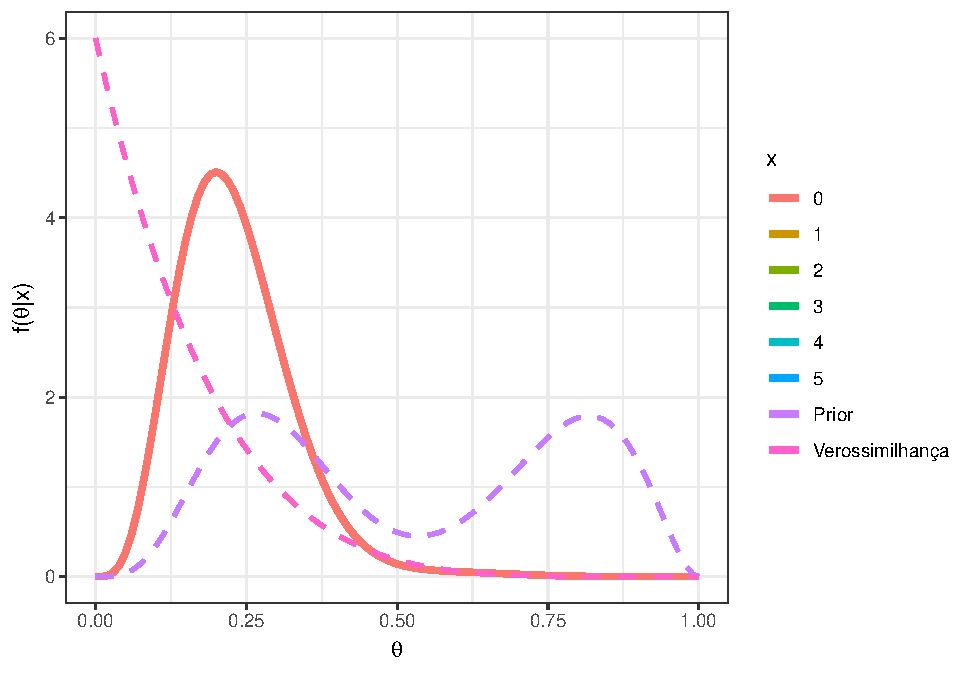
\includegraphics[width=0.8\linewidth]{InfBayes_files/figure-latex/unnamed-chunk-14-1} \end{center}

\(~\)

Agora, suponha que \(n=5\) e foi observado \(x=2\). Novamente, considere a mistura das distribuições \(Beta(5,12)\) e \(Beta(10,3)\) mas agora com pesos \(w\) variando no conjunto \(\left\{0,0.1,\ldots,0.9,1\right\}\).

\begin{Shaded}
\begin{Highlighting}[]
\NormalTok{n=}\DecValTok{5}\NormalTok{; x=}\DecValTok{2}
\NormalTok{w =}\StringTok{ }\KeywordTok{seq}\NormalTok{(}\DecValTok{0}\NormalTok{,}\DecValTok{1}\NormalTok{,}\FloatTok{0.1}\NormalTok{)}

\NormalTok{A =}\StringTok{ }\KeywordTok{as.vector}\NormalTok{(}\KeywordTok{apply}\NormalTok{(}\KeywordTok{matrix}\NormalTok{(w),}\DecValTok{1}\NormalTok{,}
  \ControlFlowTok{function}\NormalTok{(w)\{w}\OperatorTok{*}\KeywordTok{choose}\NormalTok{(n,x)}\OperatorTok{*}\KeywordTok{gamma}\NormalTok{(a1}\OperatorTok{+}\NormalTok{b1)}\OperatorTok{/}\NormalTok{(}\KeywordTok{gamma}\NormalTok{(a1)}\OperatorTok{*}
\StringTok{    }\KeywordTok{gamma}\NormalTok{(b1))}\OperatorTok{*}\NormalTok{(}\KeywordTok{gamma}\NormalTok{(a1}\OperatorTok{+}\NormalTok{x)}\OperatorTok{*}\KeywordTok{gamma}\NormalTok{(b1}\OperatorTok{+}\NormalTok{n}\OperatorTok{-}\NormalTok{x))}\OperatorTok{/}\KeywordTok{gamma}\NormalTok{(a1}\OperatorTok{+}\NormalTok{b1}\OperatorTok{+}\NormalTok{n)\}))}

\NormalTok{B =}\StringTok{ }\KeywordTok{as.vector}\NormalTok{(}\KeywordTok{apply}\NormalTok{(}\KeywordTok{matrix}\NormalTok{(w),}\DecValTok{1}\NormalTok{,}
  \ControlFlowTok{function}\NormalTok{(w)\{(}\DecValTok{1}\OperatorTok{-}\NormalTok{w)}\OperatorTok{*}\KeywordTok{choose}\NormalTok{(n,x)}\OperatorTok{*}\KeywordTok{gamma}\NormalTok{(a2}\OperatorTok{+}\NormalTok{b2)}\OperatorTok{/}\NormalTok{(}\KeywordTok{gamma}\NormalTok{(a2)}\OperatorTok{*}
\StringTok{    }\KeywordTok{gamma}\NormalTok{(b2))}\OperatorTok{*}\NormalTok{(}\KeywordTok{gamma}\NormalTok{(a2}\OperatorTok{+}\NormalTok{x)}\OperatorTok{*}\KeywordTok{gamma}\NormalTok{(b2}\OperatorTok{+}\NormalTok{n}\OperatorTok{-}\NormalTok{x))}\OperatorTok{/}\KeywordTok{gamma}\NormalTok{(a2}\OperatorTok{+}\NormalTok{b2}\OperatorTok{+}\NormalTok{n)\}))}

\NormalTok{w2 =}\StringTok{ }\NormalTok{A}\OperatorTok{/}\NormalTok{(A}\OperatorTok{+}\NormalTok{B)}

\NormalTok{prior2 =}\StringTok{ }\KeywordTok{as.vector}\NormalTok{(}\KeywordTok{apply}\NormalTok{(}\KeywordTok{matrix}\NormalTok{(w),}\DecValTok{1}\NormalTok{,}\ControlFlowTok{function}\NormalTok{(w)\{}
\NormalTok{  w}\OperatorTok{*}\KeywordTok{dbeta}\NormalTok{(theta,a1,b1)}\OperatorTok{+}\NormalTok{(}\DecValTok{1}\OperatorTok{-}\NormalTok{w)}\OperatorTok{*}\KeywordTok{dbeta}\NormalTok{(theta,a2,b2)\}))}

\NormalTok{post2 =}\StringTok{ }\KeywordTok{as.vector}\NormalTok{(}\KeywordTok{as.matrix}\NormalTok{(}\KeywordTok{mapply}\NormalTok{(}\ControlFlowTok{function}\NormalTok{(w,w2)\{}
\NormalTok{  w2}\OperatorTok{*}\KeywordTok{dbeta}\NormalTok{(theta,a1}\OperatorTok{+}\NormalTok{x,b1}\OperatorTok{+}\NormalTok{n}\OperatorTok{-}\NormalTok{x)}\OperatorTok{+}
\StringTok{  }\NormalTok{(}\DecValTok{1}\OperatorTok{-}\NormalTok{w2)}\OperatorTok{*}\KeywordTok{dbeta}\NormalTok{(theta,a2}\OperatorTok{+}\NormalTok{x,b2}\OperatorTok{+}\NormalTok{n}\OperatorTok{-}\NormalTok{x)\},w,w2)))}

\NormalTok{vero =}\StringTok{ }\KeywordTok{as.vector}\NormalTok{(}\KeywordTok{apply}\NormalTok{(}\KeywordTok{matrix}\NormalTok{(}\KeywordTok{rep}\NormalTok{(x,}\DecValTok{2}\OperatorTok{*}\NormalTok{n}\OperatorTok{+}\DecValTok{1}\NormalTok{)),}\DecValTok{1}\NormalTok{,}
  \ControlFlowTok{function}\NormalTok{(x)\{}\KeywordTok{dbeta}\NormalTok{(theta,x}\OperatorTok{+}\DecValTok{1}\NormalTok{,n}\OperatorTok{-}\NormalTok{x}\OperatorTok{+}\DecValTok{1}\NormalTok{)\}))}

\NormalTok{z<-}\KeywordTok{length}\NormalTok{(w)}

\KeywordTok{tibble}\NormalTok{(}\DataTypeTok{w=}\KeywordTok{as.factor}\NormalTok{(}\KeywordTok{rep}\NormalTok{(w,}\DataTypeTok{each=}\KeywordTok{length}\NormalTok{(theta))),}
    \DataTypeTok{w2=}\KeywordTok{rep}\NormalTok{(w2,}\DataTypeTok{each=}\KeywordTok{length}\NormalTok{(theta)),}
    \DataTypeTok{theta=}\KeywordTok{rep}\NormalTok{(theta,z), }\DataTypeTok{prior =}\NormalTok{ prior2, }
    \DataTypeTok{post =}\NormalTok{ post2, }\DataTypeTok{vero =}\NormalTok{ vero) }\OperatorTok\StringTok{ }
\StringTok{  }\KeywordTok{ggplot}\NormalTok{(}\DataTypeTok{colour =}\NormalTok{ w) }\OperatorTok{+}\StringTok{ }
\StringTok{  }\KeywordTok{geom_line}\NormalTok{(}\KeywordTok{aes}\NormalTok{(}\DataTypeTok{x=}\NormalTok{theta,}\DataTypeTok{y=}\NormalTok{post, }\DataTypeTok{colour=}\NormalTok{w),}\DataTypeTok{lwd=}\FloatTok{1.5}\NormalTok{) }\OperatorTok{+}\StringTok{ }
\StringTok{  }\KeywordTok{geom_line}\NormalTok{(}\KeywordTok{aes}\NormalTok{(}\DataTypeTok{x=}\NormalTok{theta,}\DataTypeTok{y=}\NormalTok{prior,}\DataTypeTok{colour=}\StringTok{"Priori"}\NormalTok{)) }\OperatorTok{+}
\StringTok{  }\KeywordTok{geom_line}\NormalTok{(}\KeywordTok{aes}\NormalTok{(}\DataTypeTok{x=}\NormalTok{theta,}\DataTypeTok{y=}\NormalTok{vero,}\DataTypeTok{colour=}\StringTok{"Verossimilhança"}\NormalTok{),}\DataTypeTok{lwd=}\DecValTok{1}\NormalTok{,}\DataTypeTok{lty=}\DecValTok{2}\NormalTok{)}\OperatorTok{+}
\StringTok{  }\KeywordTok{xlab}\NormalTok{(}\KeywordTok{expression}\NormalTok{(theta)) }\OperatorTok{+}\StringTok{ }\KeywordTok{ylab}\NormalTok{(}\KeywordTok{expression}\NormalTok{(}\KeywordTok{paste}\NormalTok{(}\StringTok{"f("}\NormalTok{,theta,}\StringTok{"|x)"}\NormalTok{)))}\OperatorTok{+}
\StringTok{  }\KeywordTok{theme_bw}\NormalTok{()}
\end{Highlighting}
\end{Shaded}

\begin{center}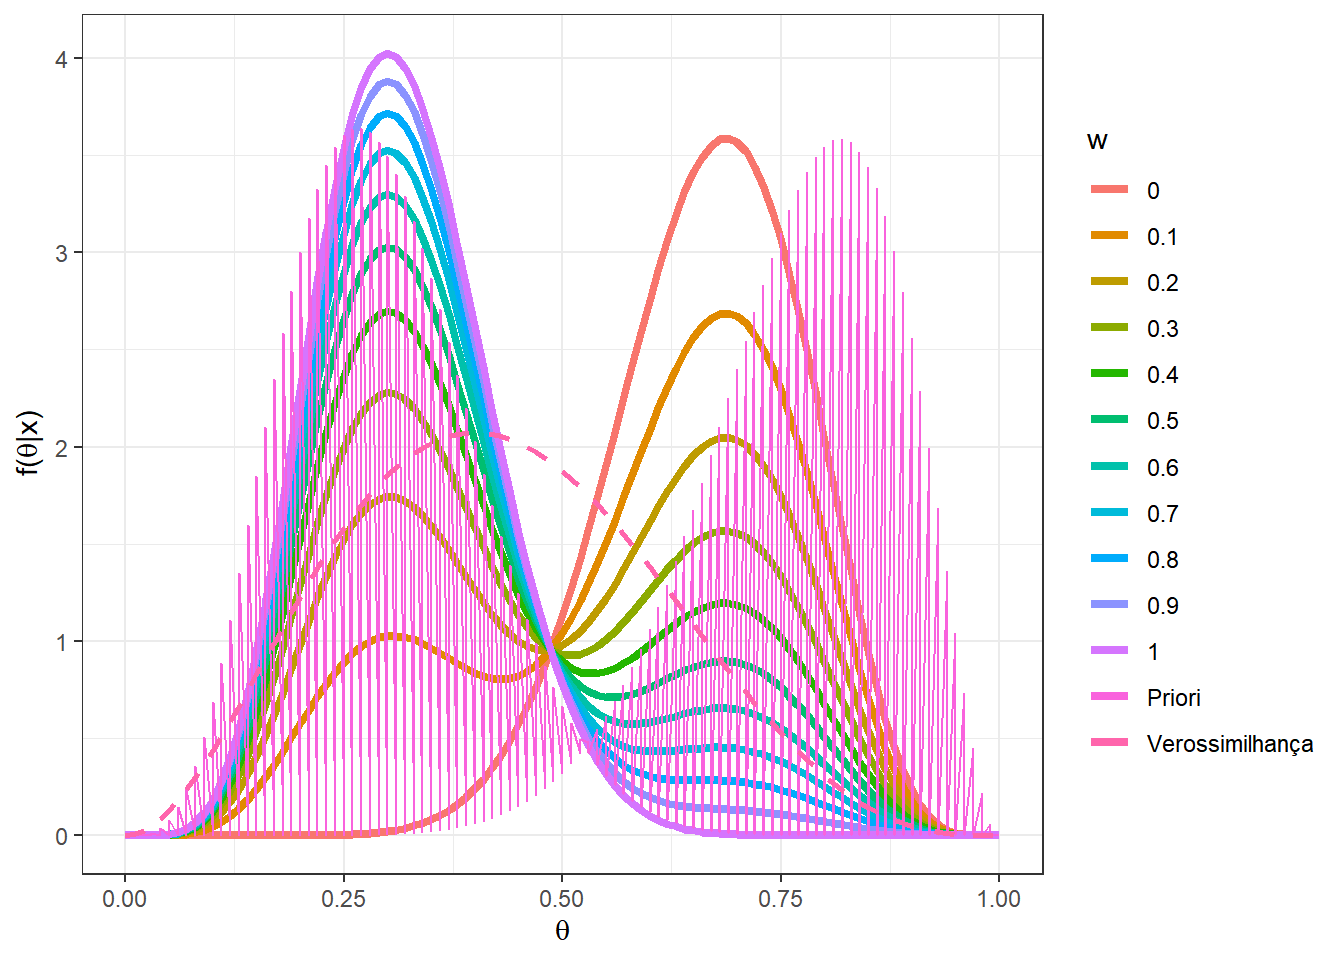
\includegraphics[width=0.8\linewidth]{InfBayes_files/figure-latex/unnamed-chunk-16-1} \end{center}

\(~\)

\(~\)

\hypertarget{prioris-nuxe3o-informativas}{%
\subsection{Prioris ``Não-Informativas''}\label{prioris-nuxe3o-informativas}}

\hypertarget{priori-de-bayes-laplace}{%
\subsubsection{Priori de Bayes-Laplace}\label{priori-de-bayes-laplace}}

\textbf{Princípio da Razão Insuficiente.} \emph{Quando não existe razão suficiente para acreditar mais em algum subconjunto do espaço paramétrico \(\Theta\), deve-se adotar equiprobabilidade.}

\(~\)

\begin{quote}
\textbf{Exemplo 1.} Se \(\Theta=\left\{\theta_1,\theta_2,\ldots,\theta_k\right\}\) então a priori de Bayes-Laplace é \(f(\theta)=1/k\), \(\theta \in \Theta~.\)
\end{quote}

\(~\)

\begin{quote}
\textbf{Exemplo 2.} Se \(\Theta=\left[a,b\right]\) então a priori de Bayes-Laplace é \(f(\theta)=1/(b-a)\), \(\theta \in \Theta~.\)
\end{quote}

\(~\)

\(f(\theta|\boldsymbol{x})\)
\(= \dfrac{f(\theta)f(\boldsymbol{x}|\theta)}{\int_\Theta f(\theta)f(\boldsymbol{x}|\theta)~d\theta}\)
\(= \dfrac{c~f(\boldsymbol{x}|\theta)}{c~\int_\Theta f(\boldsymbol{x}|\theta)~d\theta}\)
\(= \dfrac{f(\boldsymbol{x}|\theta)}{\int_\Theta f(\boldsymbol{x}|\theta)~d\theta}\)
\(\propto f(\boldsymbol{x}|\theta)~.\)

\(~\)

As principais críticas da priori de Bayes-Laplace são

\begin{enumerate}
\def\labelenumi{\arabic{enumi}.}
\item
  A distribuição é \emph{imprópria} quando o espaço paramétrico \(\Theta\) não é finito ou limitado. Por exemplo, \(\Theta=\mathbb{N}\), \(\Theta=\mathbb{Z}\) ou \(\Theta=\mathbb{R}\). Nesses casos, a priori de Bayes-Laplace é \(f(\theta)\propto \mathbb{I}_\Theta(\theta)\), que não é uma distribuição de probabilidade.
\item
  Não é \emph{invariante} a reparametrizações. Considere, por exemplo, \(f(\theta)\) uma f.d.p. a priori para \(\theta\) e \(g\) uma transformação um-a-um (injetora) de \(\theta\) tal que \(\psi=g(\theta)\). A distribuição de \(\psi\) pode ser calculada por \(f_\psi(\psi) = f\left(g^{-1}(\psi)\right)\left|\dfrac{dg^{-1}(\psi)}{d\psi}\right|~.\) Assim, se \(g\) é uma transformação não linear e a distribuição a priori para \(\theta\) é uniforme, a distribuição para \(\psi\) não é uniforme, em geral.
\end{enumerate}

\(~\)

\hypertarget{priori-de-jeffreys}{%
\subsubsection{Priori de Jeffreys}\label{priori-de-jeffreys}}

Seja \(g\) uma transformação um-a-um do parâmetro \(\theta\) e defina \(\psi=g(\theta)\). Considere uma função \(h:\mathfrak{X}\times\Theta\longrightarrow\mathbb{R}\). Uma classe de distribuições a priori invariantes pode ser definida por
\[f(\theta) \propto \left(\text{Var}_{X|\theta}\left[\dfrac{\partial h(\boldsymbol X | \theta)}{\partial\theta}~\bigg|~\theta\right]\right)^{1/2}~.\]

\begin{quote}
\textbf{Demo.} Para mostrar a invariância do método, considere o caso contínuo em que
\[f_\psi(\psi) = f\left(g^{-1}(\psi)\right)\left|\dfrac{\partial g^{-1}(\psi)}{\partial\psi}\right|~.\]
Seja \(h^*(x,\psi)=h\left(x,g^{-1}(\psi)\right)\). Então\\
\(\dfrac{\partial h^*(x,\psi)}{\partial\psi}\)
\(=\dfrac{\partial h\left(x,g^{-1}(\psi)\right)}{\partial\psi}\)
\(=\left.\dfrac{\partial h(x,\theta)}{\partial\theta}\right|_{\theta=g^{-1}(\psi)}\cdot\dfrac{\partial g^{-1}(\psi)}{\partial\psi}~,\)\\
e, portanto,\\
\(\text{Var}\left[\dfrac{\partial h^*(\boldsymbol{X},\psi)}{\partial\psi}~\bigg|~\theta=g^{-1}(\psi)\right]\)
\(=\text{Var}\left[\dfrac{\partial h(\boldsymbol{X},\theta)}{\partial\theta}~\bigg|~\theta=g^{-1}(\psi)\right]\cdot\left[\dfrac{\partial g^{-1}(\psi)}{\partial\psi}\right]^2\)
\(=\left[f\left(g^{-1}(\psi)\right)\left(\dfrac{\partial g^{-1}(\psi)}{\partial\psi}\right)\right]^2~,\)\\
de modo que\\
\(f_\psi(\psi)\) \(=f\left(g^{-1}(\psi)\right)\left|\dfrac{\partial g^{-1}(\psi)}{\partial\psi}\right|\)
\(=\text{Var}\left[\dfrac{\partial h^*(\boldsymbol{X},\psi)}{\partial\psi}~\bigg|~\theta=g^{-1}(\psi)\right]^{1/2}~.\)
\end{quote}

\(~\)

A escolha mais usual para \(h\) é \(h(\boldsymbol{x},\theta)=\log f(\boldsymbol{x}|\theta)~.\) Assim, como \(E\left[\dfrac{\partial \log f(\boldsymbol{X}|\theta)}{\partial\theta}~\bigg|~\theta\right]=0\), temos\\
\(f(\theta)\)
\(\propto\text{Var}\left[\dfrac{\partial \log f(\boldsymbol{X}|\theta)}{\partial\theta}~\bigg|~\theta\right]^{1/2}\)
\(=\text{E}\left[\left(\dfrac{\partial \log f(\boldsymbol{X}|\theta)}{\partial\theta}\right)^2~\bigg|~\theta\right]^{1/2}\)
\(=\left[\mathcal{I}(\theta)\right]^{1/2}~,\)\\
onde \(\mathcal{I}(\theta)\) é a \emph{Informação de Fisher} de \(\theta\). Neste caso, \(f(\theta)\propto\left[\mathcal{I}(\theta)\right]^{1/2}\) é chamada \textbf{priori de Jeffreys}.

\(~\)

\begin{quote}
\textbf{Exemplo 1.} Considere novamente o experimento de lançar uma moeda \(n\) vezes e contar o número de caras, isto é, \(X|\theta \sim \text{Bin}(n,\theta)\). Então,\\
\(f(x|\theta)=\displaystyle\binom{n}{x}\theta^x(1-\theta)^{n-x}\)
\(\Longrightarrow~ \log f(x|\theta)=\log\binom{n}{x}+x\log\theta+(n-x)\log(1-\theta)\)\\
\(~\)\\
\(\dfrac{\partial\log f(x|\theta)}{\partial\theta}\)
\(=\dfrac{x}{\theta}-\dfrac{n-x}{1-\theta}\)
\(=\dfrac{x-n\theta}{\theta(1-\theta)}~.\)\\
\(~\)\\
Como \(E\left[X|\theta\right]=n\theta\) e \(Var(X|\theta)\) \(=E\left[\left(X-E\left[X|\theta\right]\right)^2~\Big|~\theta\right]\) \(=E\left[\left(X-n\theta\right)^2~\Big|~\theta\right]\) \(=n\theta(1-\theta)\), a informação de Fisher neste caso é\\
\(\mathcal{I}_x(\theta)\) \(=\text{E}\left[\left(\dfrac{\partial\log f(x|\theta)}{\partial\theta}\right)^2~\bigg|~\theta\right]\) \(=\text{E}\left[\left(\dfrac{X-n\theta}{\theta(1-\theta)}\right)^2~\bigg|~\theta\right]\)
\(=\dfrac{1}{\theta^2(1-\theta)^2}~\text{E}\left[\left(X-n\theta\right)^2~|~\theta\right]\)
\(=\dfrac{1}{\theta^2(1-\theta)^2}~\text{Var}\left(X~|~\theta\right)\)
\(=\dfrac{n~\theta(1-\theta)}{\theta^2(1-\theta)^2}\)
\(=\dfrac{n}{\theta(1-\theta)}\) \(=n\theta^{-1}(1-\theta)^{-1}~,\)\\
\(~\)\\
de modo que a priori de Jeffreys é\\
\(f(\theta)\) \(\propto\left[\mathcal{I}_x(\theta)\right]^{1/2}\)
\(\propto\theta^{-1/2}(1-\theta)^{-1/2}~.\)
\end{quote}

\(~\)

\begin{quote}
\textbf{Exemplo 2.} Considere agora que a mesma moeda é lançada e anota-se o número de caras \(Y\) até que sejam observadas \(r\) coroas, isto é, \(Y|\theta \sim \text{BinNeg}(r,\theta)\). Então,
\(f(y|\theta)=\displaystyle\binom{y+r-1}{y}\theta^y(1-\theta)^{r}\)
\(\Longrightarrow~ \log f(y|\theta)=\log\binom{y+k-1}{y}+y\log\theta+r\log(1-\theta)\)\\
\(~\)\\
\(\dfrac{\partial\log f(y|\theta)}{\partial\theta}\)
\(=\dfrac{y}{\theta}-\dfrac{r}{1-\theta}\)
\(=\dfrac{1}{\theta}\left[y-\dfrac{r~\theta}{1-\theta}\right]~.\)\\
\(~\)\\
Como \(E\left[X|\theta\right]=\dfrac{r~\theta}{1-\theta}\) e \(Var(X|\theta)=\dfrac{r~\theta}{(1-\theta)^2}\), a informação de Fisher neste caso é\\
\(\mathcal{I}_y(\theta)\) \(=\text{E}\left[\dfrac{1}{\theta^2}\left(y-\dfrac{r~\theta}{1-\theta}\right)^2~\bigg|~\theta\right]\)
\(=\dfrac{1}{\theta^2}~\text{Var}\left(Y~|~\theta\right)\)
\(=\dfrac{r}{\theta(1-\theta)^2}\) \(=r\theta^{-1}(1-\theta)^{-2}~,\)\\
\(~\)\\
de modo que a priori de Jeffreys é\\
\(f(\theta)\) \(\propto\left[\mathcal{I}_y(\theta)\right]^{1/2}\)
\(\propto\theta^{-1/2}(1-\theta)^{-1}~.\)
\end{quote}

\(~\)

Note que nos exemplos apresentados, a priori depende da \emph{regra de parada}, isto é, a forma como decidimos quando parar de lançar a moeda e que determina se o modelo estatístico é binomial ou binomial negativo. Em outras palavras, a opinião a priori definida dessa forma depende do modelo adotado, mesmo que o parâmetro seja o mesmo nos dois casos.

\(~\)

\hypertarget{priori-de-muxe1xima-entropia}{%
\subsubsection{Priori de Máxima Entropia}\label{priori-de-muxe1xima-entropia}}

\textbf{Entropia} é um conceito físico que quantifica a desordem ou imprevisibilidade de um sistema, ou da falta de informação sobre ele. O conceito de entropia desempenha um importante papel na teoria da informação. O \emph{princípio da máxima entropia} afirma que a distribuição de probabilidade que melhor representa a falta de informação é aquela com a maior entropia.

\textbf{Caso Discreto.} Considere um espaço paramétrico enumerável \(\Theta = \{\theta_1,\theta_2,\ldots\}\). A \emph{entropia} da distribuição \(h\) \citep{Shannon48} é dada por

\[\mathcal{E}(h)=\text{E}[-\log h(\theta)]=\displaystyle-\sum_{\theta\in\Theta} \log\left[h(\theta)\right]~h(\theta)~.\]

\(~\)

\textbf{Definição.} Considere um espaço paramétrico \(\Theta\) e \(h\) uma f.d.p. para \(\theta\). A \emph{distribuição da máxima entropia} para \(\theta\) é a função \(h\) que maximiza \(\mathcal{E}(h)\) \citep{Jaynes03}

\(~\)

\begin{quote}
\textbf{Exemplo 1.} Considere o espaço paramétrico \(\Theta=\{\theta_1,\ldots,\theta_k\}\) e \(h(\theta_i)=p_i\) uma distribuição discreta para \(\theta\). A \emph{distribuição da máxima entropia} para \(\theta\) é a função \(h\) que maximiza \(\mathcal{E}(h)=-\displaystyle\sum_{i=1}^{k} p_i\log(p_i)\) com a restrição \(\displaystyle\sum_{i=1}^k h(\theta_i)=\sum_{i=1}^k p_i=1~.\)\\
Utilizando o método de multiplicadores de Lagrange, deve-se maximizar a função lagrangiana\\
\(\mathcal{E}^*(h)=\displaystyle-\sum_{i=1}^k p_i\log(p_i)+\lambda\left(\sum_{i=1}^k p_i-1\right)\)\\
\(\dfrac{\partial\mathcal{E}^*(h)}{\partial p_i}=-\left[p_i~\dfrac{1}{p_i}+\log(p_i)\right]+\lambda=0\) \(\Longleftrightarrow p_i = e^{\lambda-1}~~,~~~i=1,\ldots,k~.\)\\
Assim, como \(p_i\) deve ser constante e \(\sum p_i=1\), conclui-se que \(p_i=1/k\), para \(i=1,\ldots,k~.\)
\end{quote}

\(~\)

\begin{quote}
\textbf{Exemplo 2.} Considere agora \(\Theta = \{\theta_1,\theta_2,\ldots\}\) e suponha que há \(m\) informações parciais a respeito do parâmetro \(\theta\) que podem ser escritas como \(\text{E}[g_j(\theta)]=\mu_j~,~\) \(j=1,\ldots,m~.\)\\
Usando novamente o método de Lagrange, deve-se maximizar\\
\(\mathcal{E}^*(h)\) \(=\displaystyle\sum_{i=1}^\infty p_i\log(p_i)+\lambda\left(\sum_{i=1}^\infty p_i-1\right)+ \sum_{j=1}^m\lambda_j\left(\sum_{i=1}^\infty p_i~g_j(\theta_i)-\mu_j\right)\)\\
\(\dfrac{\partial \mathcal{E}^*(h)}{\partial p_i}=\displaystyle-\log(p_i)-1+\lambda+\sum_{j=1}^m\lambda_j~g_j(\theta_i)=0\)
\(\Longleftrightarrow p_i \propto e^{\lambda-1+\sum_{j=1}^m \lambda_j~g_j(\theta_i)}\) \(\propto e^{\sum_{j=1}^m \lambda_j~g_j(\theta_i)}~~,~~~i=1,\ldots,k~.\)\\
Como \(\sum p_i=1\), \(p_i = \dfrac{e^{\sum_{j=1}^m \lambda_j~g_j(\theta_i)}}{\sum_{i=1}^\infty e^{\sum_{j=1}^m \lambda_j~g_j(\theta_i)}}~\) e \(\lambda_j\) é obtido por meio das restrições.
\end{quote}

\(~\)

\begin{quote}
\textbf{Exemplo 2a.} Seja \(\Theta = \{0,1,2,\ldots\}\) e suponha que \(\text{E}[\theta]=\mu.\)\\
Usando o resultado do exemplo anterior com \(g(\theta)=\theta\) e \(\theta_i=i\), \(i=0,1,2,\ldots~,\)\\
\(p_i=\dfrac{e^{\sum_{j=1}^m \lambda_j~g_j(\theta_i)}}{\sum_{i=0}^\infty e^{\sum_{j=1}^m \lambda_j~g_j(\theta_i)}}\)
\(=\dfrac{e^{\lambda~i}}{\sum_{i=0}^\infty e^{\lambda~i}}~\)
\(\overset{\left|e^\lambda\right|<1}{=}~\dfrac{e^{\lambda~i}}{1/\left(1-e^\lambda\right)}\)
\(=\left(e^\lambda\right)^i\left(1-e^\lambda\right)\)
\(\Longrightarrow \theta \sim \text{Geo}\left(1-e^\lambda\right)~.\)\\
Como \(\text{E}\left[\theta\right]=\dfrac{e^\lambda}{\left(1-e^\lambda\right)}=\mu\), tem-se que \(\lambda=\log\dfrac{\mu}{1+\mu}~.\)
\end{quote}

\(~\)

\begin{quote}
\textbf{Exemplo 2b.} Considere que \(\Theta = \{1,2,\ldots,k\}\) e suponha que \(\text{Med}(\theta)=m~.\)\\
Nesse caso, \(g(\theta)=\mathbb{I}\left(\theta\leq m\right)\) e \(\theta_i=i\), \(i=1,2,\ldots,k~,\) de modo que\\
\(\text{E}\left[g(\theta)\right]\) \(=\text{E}\left[\mathbb{I}(\theta\leq m)\right]\) \(=\text{P}\left(\theta\leq m\right)=1/2\) e, portanto, \(\displaystyle\sum_{i\leq m}p_i=\sum_{j> m}p_j=1/2~.\)
\(p_i=\dfrac{e^{\sum_{j=1}^m \lambda_j~g_j(\theta_i)}}{\sum_{i=1}^k e^{\sum_{j=1}^m \lambda_j~g_j(\theta_i)}}\)
\(=\left\{\begin{array}{lll} \dfrac{e^\lambda}{\sum_{i\leq m} e^\lambda}&,& i\leq m \\ \dfrac{1}{\sum_{i\leq m} 1}&,& i> m\end{array}\right.\)
\(=\left\{\begin{array}{lll} \dfrac{1}{2m}&,& i\leq m \\ \dfrac{1}{2(k-m)}&,& i> m\end{array}\right.\)\\
(A distribuição de \(\theta\) é uniforme por blocos.)
\end{quote}

\(~\)

\(~\)

\textbf{Divergência de Kullbach-Leibler.} Considere duas distribuições discretas \(\boldsymbol{p} = (p_1,\ldots,p_k)\) e \(\boldsymbol{q} = (q_1,\ldots,q_k)~,\) tal que \(p_i,q_i>0~,\) \(i=1,\ldots,k~,\) e \(\sum p_i=\sum q_i=1\). A \emph{divergência de Kullbach-Leibler} entre \(\boldsymbol{p}\) e \(\boldsymbol{q}\) \citep{Kullback51} é dada por\\
\[D(\boldsymbol{p}~||~\boldsymbol{q})=\sum p_i\log\left(\dfrac{p_i}{q_i}\right)~.\]

\(~\)

Suponha que \(g=(1/k,\ldots,1/k)\)

\(D(\boldsymbol{p}~||~\boldsymbol{q})\)
\(=\displaystyle\sum_{i=1}^{k} p_i\log\left(\dfrac{p_i}{1/k}\right)\)
\(=\displaystyle\sum_{i=1}^{k}p_i\left[ln(p_i)-ln(1/k)\right]\)
\(=\displaystyle\sum_{i=1}^kp_i ln(pi)+ln(k)\sum_{i=1}^k p_i\) \(=ln(k)-\mathcal{E}(\boldsymbol p)\)

Assim, exceto por uma constante, \(\mathcal{E}(\boldsymbol p)\) está associado com quanto a distribuição \(\boldsymbol p\) ``diverge'' da distribuição uniforme (priori de referência na ausência total de informação).

\(~\)

\textbf{Observação:} No caso geral, se \(H\) e \(H_0\) são duas medidas definidas em \(\Theta\) tais que \(H\) é absolutamente contínua com relação à \(H_0\) \((H\ll H_0)\), a divergência de Kullbach-Leibler é definida como\\
\[D(H~||~H_0)=\displaystyle\int_\Theta \log\left(\dfrac{dH}{dH_0}\right)dH~,\]
em que \(\dfrac{dH}{dH_0}\) é derivada de Radon-Nikodym. Se \(H\) e \(H_0\) são medidas de probabilidade absolutamente contínuas com relação a medida de Lebesgue \(\lambda\) com f.d.p. \(\dfrac{dH}{d\lambda}=h\) e \(\dfrac{dH_0}{d\lambda}=h_0\), temos que,

\(D(H~||~H_0)\) \(=\displaystyle\int_\Theta \log\left(\dfrac{dH/d\lambda}{dH_0/d\lambda}\right)\dfrac{dH}{d\lambda}d\lambda\)
\(=\displaystyle\int_\Theta \log\left(\dfrac{h(\theta)}{h_0(\theta)}\right)h(\theta)~d\theta\)

\(~\)

\(~\)

Como a definição anterior de entropia vale apenas para o caso discreto, \citet{Jaynes03} sugere que no caso contínuo seja utilizada a \textbf{entropia relativa}, dada por
\[\mathcal{E}(h)=-\displaystyle\int_\Theta h(\theta)\log\left(\dfrac{h(\theta)}{h_0(\theta)}\right)d\theta=D(h~||~h_0)~,\]
onde \(h_0\) é uma priori de referência na ausência total de informação, preferivelmente invariante.

\(~\)

Assim como no caso discreto, se temos \(m\) restrições \(E[g_i(\theta)]=\mu_i,\) a densidade de máxima entropia é

\(h(\theta)\propto h_0(\theta)\exp\left\{\displaystyle\sum_{j=1}^m\lambda_j~ g_j(\theta)\right\}\) e os \(\lambda_j~,\) \(j=1,\ldots,m~,\) são obtidos das restrições. Por exemplo, se \(E[\theta]=\mu,\) basta fazer

\(\mu = \displaystyle \int_\Theta \theta~c~ h_0(\theta)\exp\{\lambda\theta\}~d\theta\) com \(c^{-1}=\displaystyle\int_\Theta h_0(\theta)exp\{\lambda \theta\}d\theta\).

\(~\)

\begin{quote}
\textbf{Exemplo 1:} \(\Theta = \mathbb{R}_+\) e \(\text{E}[\theta]=\mu~.\)\\
Tomando \(h_0(\theta) \propto \mathbb{I}_{\mathbb{R}_+}(\theta)\) (f.d.p. imprópria), tem-se \(h(\theta )\propto e^{\lambda\theta}~\mathbb{I}_{\mathbb{R}_+}(\theta)\) \(\propto-\lambda e^{\lambda\theta}~\mathbb{I}_{\mathbb{R}_+}(\theta)~\mathbb{I}_{\mathbb{R}_-}(\lambda)~.\)\\
Como \(\text{E}[\theta]=-1/\lambda =\mu~,\) tem-se que \(\lambda= -1/\mu\), isto é, \(\theta\sim\text{Exp}(1/\mu)~,\) de modo que \(h(\theta)=\dfrac{1}{\mu}e^{-\frac{\theta}{\mu}}~,\) \(\mu>0~.\)
\end{quote}

\(~\)

\begin{quote}
\textbf{Exemplo 2} \(\Theta = \mathbb{R}\) e \(\text{E}[\theta]=\mu\) e \(\text{Var}(\theta)=\text{E}[(\theta-\mu)^2]=\sigma^2~.\)\\
Tomando \(g_1(\theta)=\theta\) e \(g_2(\theta)=(\theta-\mu)^2\), tem-se pelo resultado anterior que\\
\(h(\theta) \propto \exp\left\{\lambda_1\theta+\lambda_2(\theta-\mu)^2\right\}\)
\(\propto \exp\left\{\lambda_1\theta+\lambda_2(\theta^2-2\theta\mu+\mu^2)\right\}\)
\(\propto \exp\left\{\lambda_2\left[\theta^2-\left(2\mu-\dfrac{\lambda_1}{\lambda_2}\right)\theta\right]\right\}\)
\(\propto \exp\left\{\lambda_2\left[\theta-\left(\mu-\dfrac{\lambda_1}{2\lambda_2}\right)\right]^2\right\}~.\)\\
Considere que \(\theta\sim N(\mu,\sigma^2)\), isto é, \(f(\theta)=\dfrac{1}{\sqrt{2\pi}~\sigma}~\exp\left\{-\dfrac{1}{2\sigma^2}(x-\mu)^2\right\}\) \(\propto \exp\left\{-\dfrac{1}{2\sigma^2}(x-\mu)^2\right\}~.\)\\
Assim, para concluir que a distribuição de máxima entropia nesse caso é a Normal anterior, basta tomar \(\mu-\dfrac{\lambda_1}{2\lambda_2}=\mu\) para ver que \(\lambda_1=0\) e \(\lambda_2=-\dfrac{1}{2\sigma^2}~.\)
\end{quote}

\(~\)

\(~\)

\(~\)

\hypertarget{alguns-princuxedpios-de-inferuxeancia}{%
\section{Alguns Princípios de Inferência}\label{alguns-princuxedpios-de-inferuxeancia}}

Considere um experimento \(E=(\boldsymbol{X},\theta,\{f(\boldsymbol x|\theta)\})\) que consiste em observar um particular valor \(\boldsymbol{x}\in\mathfrak{X}\) do v.a. \(\boldsymbol{X}\) que, para cada possível valor do parâmetro (desconhecido) \(\theta\in\Theta\), tem f.d.p. \(f(\boldsymbol x|\theta)\). De forma geral, uma \emph{inferência} sobre \(\theta\) baseada no resultado \(\boldsymbol x\) do experimento \(E\) será denotada por \(\text{Inf}(E,\boldsymbol x)~.\)

\textbf{Princípio de Suficiência.} Considere um experimento \(E=(\boldsymbol{X},\theta,\{f(\boldsymbol{x}|\theta)\})\) e suponha que \(T(\boldsymbol{X})\) é uma estatística suficiente para \(\theta\). Se \(\boldsymbol x_1\) e \(\boldsymbol x_2\) são dois pontos amostrais tais que \(T(\boldsymbol{x}_1)=T(\boldsymbol{x}_2)\) então \(\text{Inf}(E,\boldsymbol{x}_1)=\text{Inf}(E,\boldsymbol{x}_2)~.\)

\(~\)

\begin{quote}
\textbf{Exemplo 1a.} Seja \(X_1,\ldots,X_{n}\) c.i.i.d. tais que \(X_1\sim Ber(\theta)~.\)\\
Considere \(n=10\) e os pontos amostrais \(\boldsymbol x_1=(1,1,1,1,1,1,0,0,0,0)\) e \(\boldsymbol x_2=(1,0,1,0,1,0,1,0,1,1)\) tais que \(T(\boldsymbol x_1)=\sum x_{1i}=6\) e \(T(\boldsymbol x_2)=\sum x_{2i}=6\).\\
Um possível estimador para \(\theta\) nesse exemplo é a média amostral, de modo que \(\bar{x}_1=\bar{x}_2=\dfrac{\sum x_i}{n}=0,6~.\)
\end{quote}

\(~\)

\begin{quote}
\textbf{Exemplo 1b.} Ainda no contexto do exemplo anterior, considere que a priori \(\theta \sim \text{Beta}(a,b)~.\) Então, se \(T(\boldsymbol x_1)=T(\boldsymbol x_2)=t\),
\[\theta|\boldsymbol x_1\sim\theta|\boldsymbol x_2\sim\theta|T(\boldsymbol  x_1)=t~\sim~ Beta(a+t,b+n-t)~.\]
\end{quote}

\(~\)

\textbf{Princípio da Condicionalidade.} Suponha que \(E_1=\left(\boldsymbol X_1,\theta,\{f(\boldsymbol x_1|\theta)\}\right)\) e \(E_2=\left(\boldsymbol X_2,\theta,\{f(\boldsymbol x_2|\theta)\}\right)\) são dois experimentos onde somente o parâmetro \(\theta\) precisa ser comum. Considere um experimento misto em que é observada uma v.a. \(J\), com \(P(J=1)=P(J=2)=1/2\), independente de \(\boldsymbol X_1,~\boldsymbol X_2\) e \(\theta\), e então o experimento \(E_J\) é realizado. Formalmente, o experimento realizado nesse caso é \(E^*=(\boldsymbol X^*,\theta,\{f^*(\boldsymbol x^*|\theta)\})\), onde \(\boldsymbol X^*=(J,\boldsymbol X_J)\) e \(f^*(\boldsymbol x|\theta)=\dfrac{1}{2}~f_j(\boldsymbol x_j|\theta)~.\) Então, \(\text{Inf}\left(E^*,(j,x_j)\right) = \text{Inf}\left(E_j,x_j\right)~.\)

\(~\)

\textbf{Princípio da Verossimilhança.} Suponha dois experimentos \(E_1=(\boldsymbol X_1,\theta,\{f_1(\boldsymbol x_1|\theta)\})\) e \(E_2=(\boldsymbol X_2,\theta,\{f_2(\boldsymbol x_2|\theta)\})\), ambos com o mesmo parâmetro \(\theta\). Suponha que \(\boldsymbol x_1\) e \(\boldsymbol x_2\) são pontos amostrais de \(E_1\) e \(E_2\), respectivamente, tais que \(f_1(\boldsymbol x_1|\theta)\propto c(\boldsymbol x_1,\boldsymbol x_2)f_2(\boldsymbol x_2|\theta)~,\) \(\forall \theta\in\Theta~.\), então, \(\text{Inf}(E_1,\boldsymbol x_1)=\text{Inf}(E_2,\boldsymbol x_2)\).

\(~\)

\(~\)

\textbf{Teorema de Birnbaum.} (\emph{P. Suficiência} \(\wedge\) \emph{P. Condicionalidade}) \(\Longleftrightarrow\) \emph{P. Verossimilhança}.

\begin{quote}
\textbf{Demo:}\\
\((\boldsymbol{\Longrightarrow})\)\\
Seja \(\boldsymbol x_1^*,\;\boldsymbol x_2^*,\;E_1,\;E_2\) como no \emph{P. Verossimilhança} e \(E^*\) como no \emph{P. Condicionalidade}. Então,\\
\(f_1(\boldsymbol x_1|\theta)\propto c(\boldsymbol x_1,\boldsymbol x_2)f_2(\boldsymbol x_2|\theta)~.\)\\
No espaço do experimento \(E^*\), defina \(T(j,\boldsymbol{x}_j)=\left\{\begin{array}{ll}(1,\boldsymbol{x}_1^*), & \text{se } ~j=1,~\boldsymbol{x}_1=\boldsymbol{x}_1^*\\ (j,\boldsymbol{x}_j), & \text{c. c.} \end{array}\right.~.\)\\
Como \(f^*(\boldsymbol x^*|\theta)=f^*\left((j,\boldsymbol x_j)|\theta\right)=1/2~f_j(\boldsymbol x_j|\theta),\) pelo o Teorema da Fatoração é possível concluir que \(T(j,\boldsymbol x_j)\) é suficiente para \(\theta\) no experimento \(E^*\).\\
Então, pelo \emph{P. Suficiência}, \(\text{Inf}\left(E^*,(1,\boldsymbol x_1)\right)=\text{Inf}\left(E^*,(2,\boldsymbol x_2)\right)\) e, pelo \emph{P. Condicionalidade},\\
\(\text{Inf}\left(E^*,(1,\boldsymbol x_1^*)\right)\) \(=\text{Inf}\left(E_1,\boldsymbol x_1^*\right)\) \(=\text{Inf}\left(E^*,(2,\boldsymbol x_2)\right)\) \(=\text{Inf}\left(E_2,\boldsymbol x_2^*\right)~,\)\\
de modo que \(\text{Inf}\left(E_1,\boldsymbol x_1^*\right)=\text{Inf}\left(E_2,\boldsymbol x_2^*\right)\) e, portanto, vale o \emph{P. Verossimilhança}.\\
\(~\)\\
\((\boldsymbol{\Longleftarrow})\)\\
Como vale o \emph{P. Verossimilhança}, \(f_1(x_1^*|\theta)\propto f_2(x_2^*|\theta)\) e \(\text{Inf}(E_1,x_1^*)=\text{Inf}(E_2,x_2^*)~.\)\\
Além disso, se \(x^*=(1,x_1^*)\),\\
\(f^*(x^*|\theta)\) \(=f^*\left((1,x_1^*)|\theta\right)\) \(=1/2~f_1(x_1^*|\theta)\) \(\propto f_1(x_1^*|\theta)\) \(\propto 1/2~f_2(x_2^*|\theta)\) \(=f^*\left((2,x_2^*)|\theta\right)~,\)\\
e, como vale \emph{P. Verossimilhança}, então \(\text{Inf}\left(E^*,(1,x_1^*)\right)=\text{Inf}(E_1,x_1^*)~.\)\\
Usando o mesmo argumento, se \(x^*=(2,x_2^*)\), conclui-se que \(\text{Inf}\left(E^*,(2,x_2^*)\right)=Inf(E_2,x_2^*)~.\)\\
Portando, vale o \emph{P. Condicionalidade}.\\
\(~\)\\
Pelo Teorema de Fatoração, \(f(\boldsymbol x|\theta)\) \(=g\left(T(\boldsymbol x),\theta\right)h(\boldsymbol x)\) \(\propto g\left(T(\boldsymbol x),\theta\right)~.\)\\
Se \(\boldsymbol x_1\) e \(\boldsymbol x_2\) são pontos amostrais tais que \(T(\boldsymbol x_1)=T(\boldsymbol x_2),\) \(f_1(\boldsymbol x_1|\theta)\propto g\left(T(\boldsymbol x_1),\theta\right)\) \(\propto g(T(\boldsymbol x_2),\theta)\) \(\propto f_2(\boldsymbol x_2|\theta)~,\) tem-se, pelo \emph{P. Verossimilhança}, que \(\text{Inf}(E_1,\boldsymbol x_1)=\text{Inf}(E_2,\boldsymbol x_2)\) e, portanto vale o \emph{P. Suficiência}.
\end{quote}

\(~\)

\(~\)

\begin{quote}
\textbf{Exemplo.} Seja \(X_1|\theta \sim Bin(n,\theta)\) e \(X_2|\theta \sim BinNeg(r,\theta)\), onde \(n\) é número total de lançamentos (fixado) e \(r\) é número de fracassos (fixado). Então, \(E_1=\left(\boldsymbol X_1,\theta,\left\{\binom{n}{x_1}\theta^{x_1}(1-\theta)^{n-x_1}:\theta\in[0,1]\right\}\right)\) e \(E_2=\left(\boldsymbol X_2,\theta,\left\{\binom{r+x_2-1}{x_2}\theta^{x_2}(1-\theta)^{r}:\theta\in[0,1]\right\}\right)~.\) Note que em ambos os experimentos, o parâmetro \(\theta\) é o mesmo!\\
\(~\)\\
\(~\)\\
\textbf{(I)} Estimação pontual usando Estimador Não-Viesado (ENV) para \(\theta\), isto é, \(\hat{\theta}_i(X_i)\) tal que \(E\left[\hat{\theta}_i(X_i)|\theta\right]=\theta\). Nesse caso, \(\text{Inf}(E_i,x_i)=\hat{\theta}_i(x_i)\) para \(i=1,2\).\\
Então, \(\hat{\theta}_1(X_i)=\dfrac{X_1}{n}\) e \(\hat{\theta_2}(X_2)=\dfrac{X_2-1}{X_2+r-1}\) são ENV para \(\theta\) em \(E_1\) e \(E_2\), respectivamente.\\
Suponha que \(n=12,r=3\) e \(x_1=x_2=9\). Então, as funções de verossimilhança são \(f_1(x_1|\theta)=\binom{12}{9}\theta^9(1-\theta)^3\) \(\propto \binom{11}{9}\theta^9(1-\theta)^3=f_2(x_2|\theta)\). Contudo, \(\hat{\theta}_1(x_1)=\dfrac{9}{12}=0,75\) \(\neq\hat{\theta}_2(x_2)=\dfrac{8}{11}\approx0,72\bar{72}\), e portanto, o ENV \textbf{viola} o \emph{P. Verossimilhança}.\\
\(~\)\\
\(~\)\\
\textbf{(II)} Estimador de Máxima Verossimilhança (EMV)\\
\(\delta_{MV}\) é um estimador tal que \(\delta_{MV}(\boldsymbol x)=\displaystyle\arg\sup_{\theta\in\Theta} f(\boldsymbol x|\theta)~.\)\\
\(\delta_{MV}^1(x_1)=\dfrac{x_1}{n}\) \(=\delta^2_{MV}(x_2)=\dfrac{x_2}{x_2+r}\) \(=\dfrac{9}{12}=0,75~.\)\\
Portanto, o EMV \textbf{não viola} o \emph{P. Verossimilhança}.\\
\(~\)\\
\(~\)\\
\textbf{(III)} Suponha que deseja-se testar \(H_0:\theta\leq 1/2 \; (\Theta_0)\) contra \(H_1:\theta > 1/2 \; (\Theta_1)~,\) com \(\Theta=\Theta_0 \cup \Theta_1~.\)\\
\(\phi(x)=\left\{\begin{array}{ll} 1,& T(x)\leq c(\alpha)\\ 0,& T(x)> c(\alpha)\end{array}\right.\)\\
em que \(T\) é uma estatística de teste (isto é, valores ``grandes'' de \(T(x)\) indicam que \(x\) é ``favorável'' a \(H_0\)) e \(c(\alpha)\) é tal que \(\alpha=\displaystyle\sup_{\theta_0\in\Theta_0}\text{P}(\text{Rejeitar } H_0~|~\theta_0)\) \(\displaystyle\sup_{\theta_0\in\Theta_0}\text{P}\left(\left\{x\in\mathfrak{X} : T(x)\leq c(\alpha)\right\}~|~\theta_0\right)~.\)\\
Considere \(T(x)=RV(x)=\dfrac{\underset{\Theta_0}{sup}f(x|\theta)}{\underset{\Theta}{sup}f(x|\theta)}\), de modo que um \(p\)\emph{-value} pode ser calculado por \(p(x)=\displaystyle\sup_{\Theta_0} \text{P}\left(T(X)\geq T(x)|\theta\right)\). Assim, um teste que conduz a uma decisão equivalente ao descrito anteriormente é \emph{rejeitar} \(H_0\) se, e somente se, \(p(x)\leq \alpha\). Considere a escolha usual \(\alpha=0.05\). Então,\\
\(p_1(x_1)=P(X_1\geq 9|\theta=1/2)=0.073>0.05\Rightarrow\) Não rejeita \(H_0~.\)\\
\(p_2(x_2)=P(X_2\geq 9|\theta=1/2)=0.0327<0.05\Rightarrow\) Rejeita \(H_0~.\)\\
Portanto, o Teste da Razão de Verossimilhanças viola o \emph{P. Verossimilhança}.\\
\(~\)\\
\(~\)
\end{quote}

\begin{quote}
\textbf{(IV)} Aboragem Bayesiana \(\Rightarrow Inf(E_i,x_i)=f_i(\theta|x_i)\)\\
a) \emph{Bayesiano Subjetivista}\\
Como o parâmetro \(\theta\) é o mesmo nos dois experimentos, a priori deve ser a mesma.\\
\(f(\theta)\) não depende de \(\{f_i(\boldsymbol x|\theta):\theta\in\Theta\}\)\\
\(f(\theta|\boldsymbol x)\propto f(\theta)f(x_1|\theta)\propto f(\theta)f(x_2|\theta)\)\\
e, portanto, satisfaz o \emph{P. Verossimilhança}.\\
\(~\)\\
b) \emph{Bayesiano Objetivista} (p.e., usando priori de Jeffreys)\\
Para \(E_1\), \(f_1(\theta)\propto |I_F(\theta)|^{1/2}\propto\) \(\theta^{-1/2}(1-\theta)^{-1/2}\sim Beta (1/2,1/2)\)\\
Para \(E_2\), \(f_2(\theta)\propto\) \(\theta^{-1}(1-\theta)^{-1/2}\sim Beta (0,1/2)\) (distribuição imprópria).\\
Se o número de sucessos é \(x=x_1=x_2\) e número de fracassos é \(y=n-x_1=r\), temos que\\
\(\theta|X_1=x_1\sim Beta(x+1/2,y+1/2)~\) e \(~\theta|X_2=x_2\sim Beta(x,y+1/2)~.\)\\
Como \(f_1(x_1|\theta)\propto f_2(x_2|\theta)\) mas \(f_1(\theta)\neq f_2(\theta)\), tem-se que \(f_1(\theta|x_1)\neq f_2(\theta|x_2)\) e, portanto, esse procedimento viola o \emph{P. Verossimilhança}.
\end{quote}

\(~\)

\hypertarget{TeoDec}{%
\chapter{Introdução à Teoría da Decisão}\label{TeoDec}}

A teoria da decisão é uma das possíveis formas de embasar a inferência bayesiana. Sob essa abordagem, considera-se uma \emph{função de perda} (ou \emph{função de utilidade}) que quantifica numericamente as consequências de sua decisão para um dado valor do parâmetro. Essa quantificação de ``preferência'' é novamente subjetiva e é possível fazer uma construção de função de perda similar ao que fizemos com probabilidade. Ou seja, dado um conjunto de suposições, existe uma função de perda que representa numericamente suas preferências para cada decisão e cada possível valor do parâmetro. Essa construção não será feita aqui mas pode ser encontrada no livro \emph{Optimal Statistical Decisions} \citep{DeGroot70}.

\(~\)

\hypertarget{BasDec}{%
\section{Conceitos Básicos}\label{BasDec}}

\begin{itemize}
\item
  \(d \in \mathcal{D}:\) \textbf{decisão} - uma particular afirmação, por exemplo, sobre \(\theta\). No contexto inferencial, uma decisão pode ser uma estimativa (pontual ou intervalar) para \(\theta\) ou a escolha de uma hipótese específica em um teste de hipóteses.
\item
  \(\mathcal{D}:\) \textbf{espaço de decisões} - conjunto de todas as possíveis decisões (afirmações).
\item
  \(\theta\): \textbf{estado da natureza} - quantidade desconhecida ou parâmetro, no contexto de inferência estatística.
\item
  \(\Theta\): \textbf{espaço dos estados da natureza} - espaço paramétrico.
\end{itemize}

\(~\)

\textbf{Exemplo 1.}
Suponha que você está saindo de casa pela manhã e precisa tomar uma importante decisão: levar ou não seu guarda-chuva.

\begin{itemize}
\item
  \(\mathcal{D}=\{G,G^c\}\) , onde \(G:\) levar guarda-chuva.
\item
  \(\Theta=\{C,C^c\}\) , onde \(C:\) chuva.
\end{itemize}

Suponha que carregar o guarda-chuva é algo que não lhe agrada mas, por outro lado, você odeia ficar molhado e acredita que a pior situação seria não levá-lo e tomar chuva. Você ficará incomodado se levar o guarda-chuva e chover pois, além de tê-lo carregado, voltou para casa com os sapatos molhados. Note que, nessas circunstâncias, o cenário preferido por você seria não levar o guarda-chuva e não chover.

Para quantificar suas preferências, considere uma função de perda \(L:\mathcal{D}\times\Theta\longrightarrow\mathbb{R}\), de modo que, quanto mais algum cenário lhe gera incômodo, maior sua perda. Um exemplo é apresentado a seguir.

\begin{longtable}[]{@{}lll@{}}
\toprule
& Estados da Natureza &\tabularnewline
\midrule
\endhead
\textbf{Decisão} & \(C\) & \(C^c\)\tabularnewline
\(G\) & 2 (ruim) & 1 (bom)\tabularnewline
\(G^c\) & 3 (pior) & 0 (melhor)\tabularnewline
\(P(\theta)\) & p & 1-p\tabularnewline
\bottomrule
\end{longtable}

Uma possível maneira de tomar uma decisão é escolher a decisão ``menos prejudicial''. Se levar o Guarda chuva, no pior caso, sua perda é \(\displaystyle \max_\theta L(G,\theta)=2\) e, se não levá-lo, a maior perda possível é \(\displaystyle \max_\theta L(G^c,\theta)=3\). Assim, a decisão que tem a menor dentre as maiores perdas é levar o guarda-chuva. Esse procedimento para tomada de decisões é chamado \emph{min-max} e consiste em escolher a decisão \(d'\) tal que \(d' = \displaystyle \underset{d}{\text{argmin}} \max_\theta L(d,\theta)\).

Sendo um pouco mais otimista, você pode escolher a decisão que tenha a maior dentre as menores perdas. Esse procedimento é chamado \emph{max-min} e consiste em escolher a decisão \(d' = \displaystyle \underset{d}{\text{argmax}} \min_\theta L(d,\theta)\). No nosso exemplo, esse procedimento também sugere que você sempre carregue o guarda-chuvas.

Note que a decisão escolhida pelos dois procedimentos descritos anteriormente sugere que você sempre deve carregar o guarda-chuvas. Contudo, isso pode não ser razoável. Imagine que você estava lendo notícias antes de sair de casa e viu que a probabilidade de chuva era \(0.01\). Nesse caso, não parece fazer sentido você levar o guarda-chuva, já que isso vai te trazer um desconforto e a chance de chover é muito baixa. Assim, a probabilidade de chover deveria ser levada em consideração em sua tomada de decisão.

Uma maneira de fazer isso é utilizar a \textbf{perda esperada}. Note que \(\theta\) é uma quantidade desconhecida e, pelo que já foi discutido anteriormente, você deve descrever sua incerteza em relação a essa quantidade em termos de probabilidade. Suponha que no exemplo \(P(C)=p\), \(0\leq p\leq 1\).

\(~\)

Para cada decisão \(d \in \mathcal{D}\), é possível calcular o valor esperado da função de perda (\textbf{perda esperada} ou \textbf{risco} da decisão \(d\) contra a priori \(P\))
\[\rho(d,P) = E\left[L(d,\theta) ~|~ P\right] = \int_{\Theta} L(\theta) dP(\theta).\]
\(~\)

No exemplo, temos

\begin{itemize}
\item
  \(E\left[L(G^{},\theta)\right]\) \(=L(G,C)P(C) + L(G,C^c)P(C^c)\) \(=2p+1(1-p)\) \(=p+1\);
\item
  \(E\left[L(G^c,\theta)\right]\) \(=L(G^c,C)P(C) + L(G^c,C^c)P(C^c)\) \(=3p+0(1-p)\) \(=3p\).
\end{itemize}

Deste modo, as perdas esperadas associadas a cada decisão dependem da probabilidade de chuva \(p\). Assim, para cada possível valor de \(p\), deve-se tomar a decisão que tem menor perda esperada. Por exemplo, se a probabilidade de chuva é \(p=0.1\), temos que as perdas esperadas para as decisões de levar ou não o guarda-chuva são, respectivamente, \(E\left[L(G,\theta)\right]=1.1\) e \(E\left[L(G^c,\theta)\right]=0.3\). Assim, sob essa abordagem, sua decisão seria de não levar o guarda-chuva nesse caso. Por outro lado, se a probabilidade de chuva for \(p=0.9\), suas perdas esperadas seriam respectivamente \(E\left[L(G,\theta)\right]=1.9\) e \(E\left[L(G^c,\theta)\right]=2.7\), de modo que a decisão ótima seria levar o guarda-chuva. O gráfico a seguir apresenta as perdas para cada decisão \(d\) e para cada valor de \(p\). É possível notar que a decisão ótima é levar o guarda-chuva quando \(p>0.5\) e não levá-lo caso contrário.

\begin{center}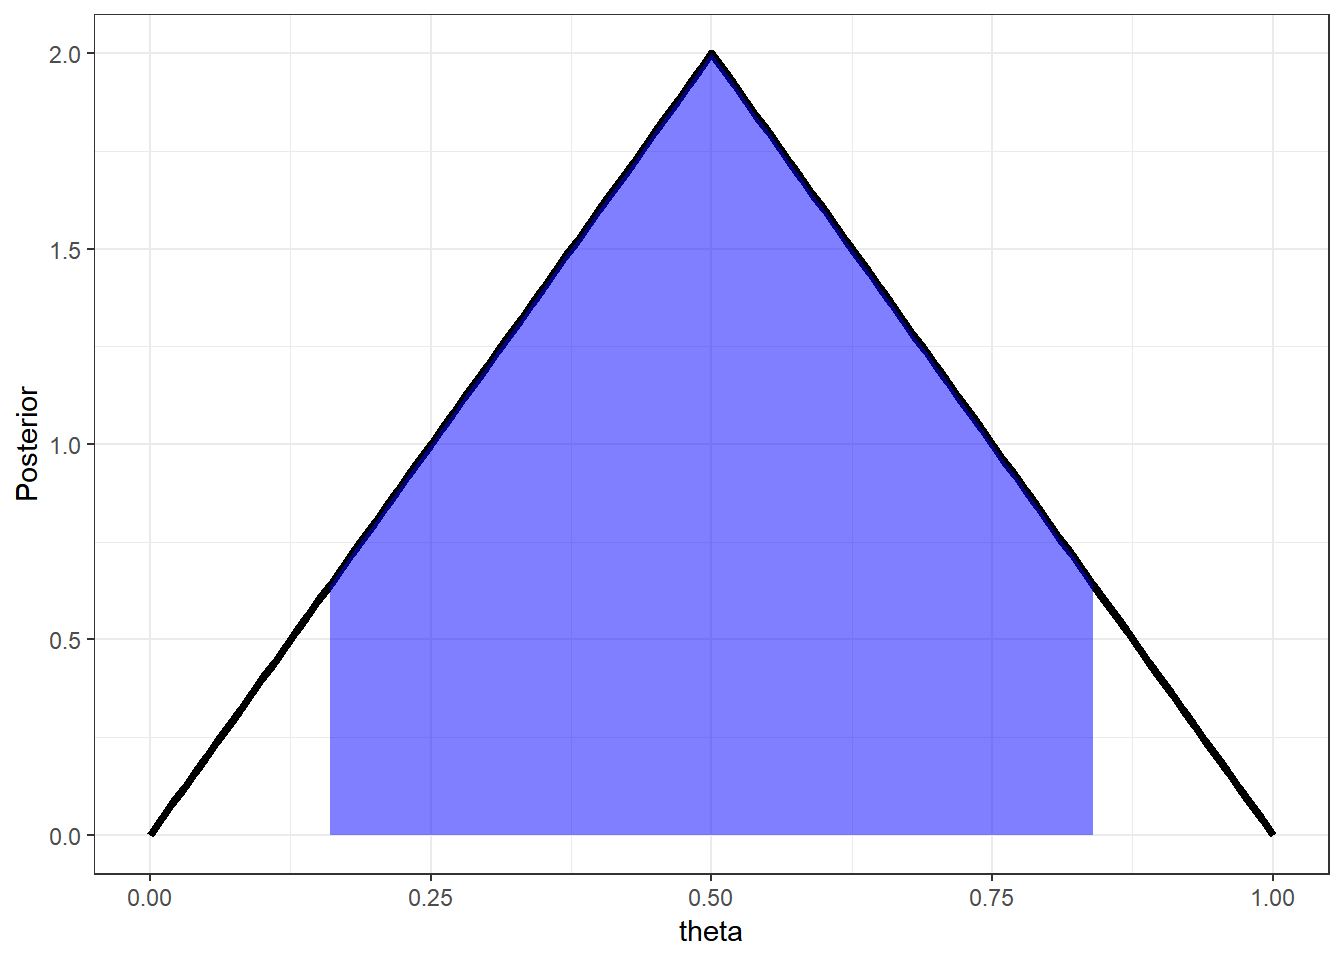
\includegraphics[width=0.8\linewidth]{InfBayes_files/figure-latex/unnamed-chunk-18-1} \end{center}

\(~\)

Vamos denotar por \(\rho^*\) o \textbf{risco de bayes}, isto é, a perda esperada da \textbf{decisão de Bayes} (ou \emph{decisão ótima}) \(d^*\in \mathcal{D}\) tal que \(\rho^*(P)\) \(=\rho(d^*,P)\) \(=\underset{d\in\mathcal{D}}{min}~\rho(d,P)\).

\(~\)

Para uma argumentação mais formal sobre a escolha pela decisão que minimiza a perda esperada, ver \emph{Optimal Statistical Decisions} (DeGroot, M.H.).

\(~\)

\(~\)

\begin{itemize}
\tightlist
\item
  Vamos denotar um problema de decisão por \(\left(\Theta, \mathcal{D}, L, P\right)\), onde \(\Theta\) é o espaço paramétrico, \(\mathcal{D}\) é o espaço de decisões, \(L: \mathcal{D} \times \Theta \longrightarrow \mathbb{R}\) é uma função de perda e \(P\) é a distribuição de probabilidade que representa sua crença sobre a quantidade desconhecida \(\theta\). Equivalentemente, a função de perda \(L\) pode ser substituída por uma \emph{função de utilidade} \(U\) (por exemplo, tome \(U=-L\)).
\end{itemize}

\(~\)

\begin{itemize}
\tightlist
\item
  A solução para um problema de decisão \(\left(\Theta, \mathcal{D}, L, P\right)\) é a \emph{decisão de Bayes}, \({d}^* \in \mathcal{D}\), tal que \(\rho^*(P) = \rho({d}^*,P) = \displaystyle \inf_{d \in \mathcal{D}} \rho(d,\theta)\), com \(\rho(d,P) = \displaystyle \int_\Theta L(d,\theta)dP(\theta)\).
\end{itemize}

\(~\)

\hypertarget{aleatorizauxe7uxe3o-e-decisuxf5es-mistas}{%
\section{Aleatorização e Decisões Mistas}\label{aleatorizauxe7uxe3o-e-decisuxf5es-mistas}}

Seja \(D=\left\{d_1,d_2,\ldots\right\}\) um espaço de decisões e considere \(\mathcal{M}\) o conjunto de todas as \emph{decisões mistas} (ou \emph{aleatorizadas}), isto é, para toda distribuição de probabilidades \(Q=\left\{q_1,q_2,\ldots\right\}\), uma decisão \(d\in\mathcal{M}\) se \(d\) consiste em escolher a decisão \(d_i\) com probabilidade \(q_i\).

Assim, a perda associada à uma decisão \(d\in\mathcal{M}\) é \(L(d,\theta) = \sum q_i L(d_i,\theta)\) e o risco dessa decisão é

\(\rho(d,P)\) \(= \displaystyle \int_\Theta L(d,\theta) dP(\theta)\) \(=\displaystyle \int_\Theta \sum q_i L(d_i,\theta) dP(\theta)\) \(=\displaystyle \sum q_i \int_\Theta L(d_i,\theta) dP(\theta)\) \(=\displaystyle \sum q_i~ \rho(d_i,\theta)\).

Considere a decisão \({d}^* \in \mathcal{D}\) tal que \(\rho({d}^*,P) = \displaystyle \inf_{d \in \mathcal{D}} \rho(d,\theta)\).

Então, \(\forall ~d \in \mathcal{M}\),

\(\rho(d,P)\) \(=\displaystyle \sum q_i~ \rho(d_i,\theta)\) \(\geq \displaystyle \sum q_i~ \rho({d}^*,\theta)\).

\begin{itemize}
\tightlist
\item
  Em palavras, para toda decisão aleatorizada \(d\in\mathcal{M}\), existe uma decisão não aleatorizada \({d}^*\in\mathcal{D} \subset\mathcal{M}\), tal que \(\rho({d}^*,P) \leq \rho(d,P)\).
\end{itemize}

\(~\)

\hypertarget{problemas-com-dados}{%
\section{Problemas com Dados}\label{problemas-com-dados}}

Suponha que antes de escolher uma decisão \(d \in \mathcal{D}\), é possível observar um v.a. \(\boldsymbol X\) que (supostamente) está relacionado com \(\theta\) (isto é, \(\boldsymbol X\) traz alguma informação sobre \(\theta\)).

Desde modo, considere a família \(\mathcal{P}=\left\{ f(\cdot|\theta) : \theta \in \Theta\right\}\) de funções de distribuição condicionais para \(\boldsymbol X\), isto é, para cada \(\theta \in \Theta\) é possível determinar a distribuição condicional de \(\boldsymbol X|\theta\). Essa distribuição, juntamente com a distribuição a priori \(f(\theta)\), determina totalmente uma distribuição conjunta \(f(\boldsymbol x,\theta) = f(\boldsymbol x|\theta) f(\theta)\).

Pode-se definir uma \textbf{função de decisão} \(\delta: \mathfrak{X} \longrightarrow \mathcal{D}\) que associa a cada resultado experimental \(\boldsymbol x \in \mathfrak{X}\) uma decisão \(d \in \mathcal{D}\). Denote o conjunto de todas as possíveis funções de decisão por \(\Delta\).

O risco \(r(\delta,P)\) da função de decisão \(\delta \in \Delta\) é dado por \(r(\delta,P)\) \(=E\left[L\left(\delta,\theta\right)\right]\) \(=\displaystyle \int_\Theta \int_{\mathfrak{X}} L\left(\delta(\boldsymbol x),\theta\right) dP(\boldsymbol x,\theta)\).

A \emph{função de decisão de Bayes}, \({\delta}^* \in \Delta\), é tal que \({\rho}^*(P)\) \(=\rho({\delta}^*,P)\) \(=\displaystyle \inf_{\delta\in \Delta} \rho(\delta,P)\).

\(~\)

\textbf{Exemplo 1.} Seja \(\Theta=\{\theta_1,\theta_2\}\), \(\mathcal{D}=\{d_1,d_2\}\), \(X|\theta_1\sim Ber(3/4)\), \(X|\theta_2 \sim Ber(1/3)\), \(\mathfrak{X}=\{0,1\}\) e, a priori, \(P(\theta=3/4)=P(\theta=1/3)=1/2\). Considere a função de perda a seguir.

\begin{longtable}[]{@{}lll@{}}
\toprule
L & \(\theta_1\) & \(\theta_2\)\tabularnewline
\midrule
\endhead
\(d_1\) & 0 & 5\tabularnewline
\(d_2\) & 10 & 0\tabularnewline
\bottomrule
\end{longtable}

Temos que \(|\Delta| = 2^2=4\), de modo que as possíveis funções de decisão são

\(\delta_1(x)=\left\{\begin{array}{lr} d_1, & x=1\\ d_2, &x=0\end{array}\right.\)

\(\delta_2(x)=\left\{\begin{array}{lr} d_1, & x=0\\ d_2, &x=1\end{array}\right.\)

\(\delta_3(x)=d_1\) e \(\delta_4(x)=d_2\).

Para a função \(\delta_1\), temos

\begin{longtable}[]{@{}llllll@{}}
\toprule
x & \(\theta\) & \(L(\delta_1(x),\theta)\) & \(P(x|\theta)\) & \(P(\theta)\) & \(P(x,\theta)\)\tabularnewline
\midrule
\endhead
0 & \(\theta_1\) & 10 & 1/4 & 1/2 & 1/8\tabularnewline
0 & \(\theta_2\) & 0 & 2/3 & 1/2 & 2/6\tabularnewline
1 & \(\theta_1\) & 0 & 3/4 & 1/2 & 3/8\tabularnewline
1 & \(\theta_2\) & 5 & 1/3 & 1/2 & 1/6\tabularnewline
\bottomrule
\end{longtable}

\(\rho(\delta_1)\) \(=\displaystyle \sum_{x=0}^1\sum_{i=1}^2L(\delta_1(x),\theta_i)\underbrace{P(X=x|\theta_i)P(\theta_i)}_{P(x,\theta)}\) \(=10~\dfrac{1}{8}+5~\dfrac{1}{6}\) \(=\dfrac{50}{24}\)

De forma análoga, \(~\rho(\delta_2,P)=130/24\) , \(~\rho(\delta_3,P)=60/24\) , \(~\rho(\delta_4,P)=120/24\) , e, assim.

\({\delta}^*(x)={\delta}^*_1(x)=\left\{\begin{array}{rl} d_1, & x=1\\ d_2, & x=0\end{array}\right.\)

\textbf{Risco de Bayes:} \(\rho^*(P)=\rho({\delta}^*,P)=50/24\).

\(~\)

Em problemas mais complicados, pode ser muito trabalhoso (ou impossível) obter a função de decisão dessa forma, chamada \emph{forma normal}. Sob essa abordagem, é necessário encontrar a função de decisão de bayes \({\delta}^*\) dentre todas as possíveis funções de decisão. Nesses casos, pode ser mais fácil resolver o problema usando a \emph{forma extensiva} em que, para cada \(\boldsymbol x \in \mathfrak{X}\), obtem-se a decisão de Bayes \({d}_{x}^*\) que minimiza o \emph{risco posterior}, definido por \(r_x(d)\) \(= \displaystyle \int_\Theta L(d,\theta) dP(\theta|\boldsymbol x)\).

Assim, é posível obter uma decisão de Bayes \({d}_x^*\) para um específico ponto \(x\) observado ou, ainda, construir uma função de decisão de Bayes, fazendo \(~{\delta}^*(\boldsymbol x) = {d}_x^*~\) para cada \(\boldsymbol x \in \mathfrak{X}\). A seguir, é mostrado que essa duas formas produzem resultados que minimizam o risco. Note que

\(r(\delta,P)\) \(=E\left[L\left(\delta,\theta\right)\right]\) \(=\displaystyle \int_\Theta \int_{\mathfrak{X}} L\left(\delta(\boldsymbol x),\theta\right) dP(\boldsymbol x,\theta)\) \(=\displaystyle \int_\Theta \int_{\mathfrak{X}} L\left(\delta(\boldsymbol x),\theta\right) dP(\boldsymbol x|\theta)dP(\theta)\) \(=\displaystyle \int_{\mathfrak{X}} \left[ \underbrace{\int_\Theta L\left(\delta(\boldsymbol x),\theta\right) dP(\theta|\boldsymbol x)}_{r_x\left(\delta(\boldsymbol x)\right)} \right]dP(\boldsymbol x)\).

Note que a integral interna (em \(\theta\)) pode ser resolvida para cada \(\boldsymbol x\) fixado. Para cada \(\boldsymbol x\), considere a decisão \({d}_x^*\) tal que \(r_x\left({d}_x^*\right)\) \(=\displaystyle \inf_{d \in \mathcal{D}} r_x(d)\). Assim

\(r(\delta,P)\) \(=\displaystyle \int_{\mathfrak{X}} \left[ \underbrace{\int_\Theta L\left(\delta(\boldsymbol x),\theta\right) dP(\theta|\boldsymbol x)}_{r_x\left(\delta(\boldsymbol x)\right)} \right]dP(\boldsymbol x)\) \(=\displaystyle \int_{\mathfrak{X}} \left[ {r_x\left(\delta(\boldsymbol x)\right)} \right]dP(\boldsymbol x)\) \(\geq \displaystyle \int_{\mathfrak{X}} \left[ {r_x\left({d}_x^*\right)} \right]dP(\boldsymbol x)\) \(= \displaystyle \int_{\mathfrak{X}} \left[ {r_x\left({d}_x^*\right)} \right]dP(\boldsymbol x)\).

Assim, a função \({\delta}^*(x)={d}^*_{x}\) é uma \emph{função de decisão de Bayes}.

\(~\)

\textbf{No Exemplo 1} \(~X|\theta_1 \sim Ber(3/4)\) , \(~X|\theta_2 \sim Ber(1/3)\) e \(~P(\theta_1)=P(\theta_2)=1/2\).

\(P(\theta_1|x=0)\) \(=\dfrac{P(X=0|\theta_1)P(\theta_1)}{P(X=0|\theta_1)P(\theta_1)+P(X=0|\theta_2)P(\theta_2)}\) \(=\dfrac{\frac{1}{4}~\frac{1}{2}}{\frac{1}{4}~\frac{1}{2}+\frac{2}{3}~\frac{1}{2}}\) \(=\dfrac{3}{11}\)

\(P(\theta_2|X=0)\) \(=\dfrac{8}{11}\)

\(r_x(d_1,P)\) \(=\displaystyle \sum_{i=1}^2L(d_1,\theta_i)P(\theta_i|X=0)\) \(=0~P(\theta_1|X=0)+10~P(\theta_2|X=0)\) \(=\dfrac{80}{11}\)

\(r_x(d_2,P)\) \(=5~P(\theta_1|X=0)+0~P(\theta_2|X=0)\) \(=\dfrac{15}{11}\)

Logo, para \(x=0\), \({d}_0^*={d}_2\). De forma análoga, para \(x=1\), \({d}_1^*={d}_2\) e, assim,

\({\delta}^*(x)=\left\{\begin{array}{rl} {d}_2, & x=0\\ {d}_1, & x=1~.\end{array}\right.\)

\(~\)

\hypertarget{Estimacao}{%
\chapter{Estimação}\label{Estimacao}}

\hypertarget{estimauxe7uxe3o-pontual}{%
\section{Estimação Pontual}\label{estimauxe7uxe3o-pontual}}

Todos os problemas de inferência estatística podem ser vistos como um caso particular de Teoria da Decisão. Um problema de estimação pontual consiste em encontrar um ``chute'' para o valor do parâmetro \(\theta\), de modo que o espaço de decisões é \(\mathcal{D}=\Theta\). Além disso, nesse tipo de problema é usual considerar funções de perda da forma \(L(d,\theta)=s(\theta)\Delta(d,\theta)\), onde \(\Delta\) é alguma distância (ou uma medida de discrepância) relacionada ao erro por tomar a decisão \(d\) quando o valor do parâmetro é \(\theta\) e \(s\) é uma função não-negativa relacionada à gravidade do erro para cada \(\theta\) (pode ser constante).

\(~\)

\textbf{Exemplo} Considere um problema de estimação pontual, isto é, \(\mathcal{D}=\Theta\), onde a função de perda é dada por \(L(d,\theta)=(d-\theta)^2\), conhecida como \emph{perda quadrática}.

\(r_x(d)\) \(=\displaystyle \int_\Theta(d-\theta)^2~dP(\theta|x)\)
\(=\displaystyle \int_\Theta \left(d^2 - 2d\theta + \theta^2\right) dP(\theta|x)\) \(=d^2\displaystyle\int_\Theta dP(\theta|x) - 2d\int_\Theta\theta ~dP(\theta|x) + \int_\Theta \theta^2 ~dP(\theta|x)\) \(=d^2-2d~E[\theta|x]+E[\theta^2|x]=g(d)\).

\(\dfrac{\partial g(d)}{\partial d}\) \(=2d-2E[\theta|x]=0\) \(\Rightarrow {d}_x^*=E[\theta|x]\).

Logo, um estimador para \(\theta\) contra a perda quadrática é \({\delta}^*(X)=E[\theta|X]\).

\(~\)

\(~\)

\begin{itemize}
\item
  Estimador de Bayes para \(\theta\) contra diferentes funções de perda:

  \begin{enumerate}
  \def\labelenumi{\arabic{enumi}.}
  \item
    Perda Quadrática: \(L_2(d,\theta)=(d-\theta)^2\) \(~\Longrightarrow~\) \({\delta}_2^*(X)=E[\theta|X]\);
  \item
    Perda Absoluta: \(L_1(d,\theta)=|d-\theta|\) \(\Longrightarrow\) \({\delta}_1^*(X)=Med(\theta|X)\);
  \item
    Perda 0-1: \(L_0(d,\theta)=c~\mathbb{I}(d\neq\theta)\) \(\Longrightarrow\) \({\delta}_0^*(X)=Moda(\theta|X)\).
  \end{enumerate}
\end{itemize}

\(~\)

\(~\)

\textbf{Exemplo 1.} Voltando à \emph{Perda Quadrática:} \(L(d,\theta)=a(d-\theta)^2\), \(a>0\).

Já vimos que \(\delta^*(\boldsymbol X)=E[\theta|\boldsymbol X]\). É importante notar que esse estimador só faz sentido se \(E[\theta|\boldsymbol X]\in \mathcal{D}\). Nos casos em que isso não ocorre, tomamos um valor \({d}_x^* \in \mathcal{D}\) próximo a \(E[\theta|\boldsymbol X]\) tal que \(r_x\left({d}_x^*\right)\) é mínimo.

\(~\)

O risco a posteriori para esse estimador é

\(r_x\left(\delta^*(\boldsymbol x)\right)\) \(=r_x\left(E[\theta|\boldsymbol x]\right)\) \(=\displaystyle \int_\Theta L\left(\delta^*(\boldsymbol x),\theta\right)dP(\theta|\boldsymbol x)\) \(=\displaystyle \int_\Theta \left(\theta-E[\theta|\boldsymbol x]\right)^2 dP(\theta|\boldsymbol x)\) \(=Var(\theta|\boldsymbol x)\),

de modo que o risco de Bayes é dado por

\({\rho}^*\left(P\right)\) \(=\rho\left(\delta^*(\boldsymbol X),P\right)\) \(=\displaystyle \int_{\mathfrak{X}} \underbrace{ \int_{\Theta}(\theta-E[\theta|\boldsymbol{x}])^2dP(\theta|\boldsymbol{x})}_{Var[\theta|\boldsymbol{x}]}dP(\boldsymbol{x})\) \(=E\left[Var(\theta|\boldsymbol X)\right]\).

A variância da posteriori \(Var(\theta|\boldsymbol x)\) pode ser vista como uma medida de informação, no sentido que quanto menor essa variância, mais concentrada é a distribuição e há ``\emph{menos incerteza}'' sobre \(\theta\). Nesse sentido, espera-se que ao observar \(\boldsymbol X=\boldsymbol x\), a variância \(Var(\theta|\boldsymbol x)\) diminua em relação a variância da priori \(Var(\theta)\).

\[\underbrace{Var(\theta)}_{constante}=\underbrace{E\left[Var(\theta|\boldsymbol X)\right]}_{\boldsymbol \Downarrow}+\underbrace{Var\left[E(\theta|\boldsymbol X)\right]}_{\boldsymbol \Uparrow}\]

Aparentemente, quando espera-se que a variância da posteriori diminua, a variância do estimador deveria aumentar. Muitas vezes isso é colocado como se o objetivo fosse encontrar o estimador de maior variância, em contradição com a abordagem frequentista. Contudo, há outra interpretação desse resultado: deseja-se obter um estimador que varie bastante de acordo com o valor observado de \(\boldsymbol X\), isto é, a informação trazida pela amostra muda sua opinião sobre \(\theta\).

\(~\)

\textbf{Exemplo 2.} Considere \(X_1,...X_n\) c.i.i.d. tais que \(X_i|\theta\sim Poisson(\theta)\) e, a priori, \(\theta \sim Gama(a,b)\).

A função de verossimilhança é \(f(\boldsymbol x | \theta)\propto \prod {\theta}^{x_i}~{e}^{-\theta}\) e a priori é \(~f(\theta)\propto{\theta}^{a-1}~{e}^{-b\theta}\).

Assim, \(f(\theta | \boldsymbol x)\) \(\propto {\theta}^{\sum x_i}~{e}^{-n\theta} ~\cdot~ {\theta}^{a-1}~{e}^{-b\theta}\) \(\propto {\theta}^{a+\sum x_i-1}~{e}^{-(b+n)\theta}\), de modo que \(\theta|\boldsymbol X=\boldsymbol x\sim Gama\left(a+\sum x_i,b+n\right)\).

Como visto anteriormente, o estimador de Bayes contra a perda quadrática é

\(\delta^*(\boldsymbol X)=E[\theta|\boldsymbol X]=\dfrac{a+\sum_iX_i}{b+n}\).

Para calcular o risco de Bayes, note que \(E[X_i|\theta]=\theta\), de modo que \(E[X_i]=E\left[E(X_i|\theta)\right]=E[\theta]=a/b\). Além disso, \(Var(\theta)=\dfrac{a}{b^2}\) e \(Var(\theta|\boldsymbol X)=\dfrac{a+\sum_iX_i}{(b+n)^2}\). Então,

\(\rho^*(P)\) \(=E\left[Var(\theta|\boldsymbol X)\right]\) \(=E\left[\dfrac{a+\sum_iX_i}{(b+n)^2}\right]\) \(= \dfrac{\left(a+\sum E[X_i]\right)}{(b+n)^2}\) \(=\dfrac{\dfrac{a}{b}\left(b+n\right)}{(b+n)^2}\) \(=\dfrac{a}{b(b+n)}\).

Por fim, note que a decisão de Bayes pode ser escrita como uma combinação linear convexa da média da distribuição a priori e do estimador de máxima verossimilhança

\(E[\theta|\boldsymbol X]\) \(=\dfrac{a+\sum_iX_i}{b+n}\) \(=\dfrac{b}{b+n}\left(\dfrac{a}{b}\right)+\dfrac{n}{b+n}\bar{X}\).

\(~\)

\textbf{Resultado:} Seja \(L(d,\theta)=\mathbb{I}(|\theta-d|> \varepsilon)\) \(=1-\mathbb{I}(d-\varepsilon\leq \theta \leq d+\varepsilon)\) , \(\varepsilon > 0\).
Então, \(\delta^*(\boldsymbol X)\) é centro do intervalo modal, isto é, o intervalo de tamanho \(2\varepsilon\) de maior densidade a posteriori. Em particular, quando \(\varepsilon \downarrow 0\), temos que \({\delta}^*(\boldsymbol X)=Moda(\theta|\boldsymbol X)\).

\textbf{Demo:} O risco posterior de uma decisão \(d\) é

\(r_{\boldsymbol{x}}(d)\) \(=E\left[L(d,\theta)|\boldsymbol{x}\right]\) \(=E\left[\mathbb{I}(|\theta-d|> \varepsilon)\right]\) \(=E\left[1-\mathbb{I}(d-\varepsilon\leq \theta \leq d+\varepsilon)|\boldsymbol x\right]\) \(=1-P(d-\varepsilon\leq \theta \leq d+\varepsilon|\boldsymbol x)\).

O risco \(r_{\boldsymbol{x}}(d)\) é mínimo quando a probabilidade \(P(d-\varepsilon\leq \theta \leq d+\varepsilon|\boldsymbol x)\) é máxima. Assim, basta tomar o intervalo \(\left[{d}_x^*-\varepsilon ~;~ {d}_x^*+\varepsilon\right]\) com maior probabilidade a posteriori e o estimador de Bayes nesse caso será o valor central desse intervalo, \({d}_x^*\).

\(~\)

\textbf{Exemplo 3.} Considere o exemplo anterior onde \(\theta|\boldsymbol x\sim Gama(a+\sum x_i,b+n)\) e a função de perda do resultado anterior, \(L(d,\theta)=\mathbb{I}(|\theta-d|> \varepsilon)\). Temos que

\(f(\theta|\boldsymbol x)\) \(\propto \theta^{\overbrace{a+\sum x_i-1}^{A_x}}e^{-\overbrace{(b+n)}^{B_x}\theta}\) \(=\theta^{A_x}e^{-{B_x}\theta}\)

\begin{Shaded}
\begin{Highlighting}[]
\NormalTok{theta =}\StringTok{ }\KeywordTok{seq}\NormalTok{(}\DecValTok{0}\NormalTok{,}\FloatTok{1.2}\NormalTok{,}\FloatTok{0.01}\NormalTok{)}
\CommentTok{#Parâmetros da dist a posteriori gama}
\NormalTok{a1 =}\StringTok{ }\DecValTok{3}
\NormalTok{b1 =}\StringTok{ }\DecValTok{10}
\NormalTok{posterior =}\StringTok{ }\KeywordTok{dgamma}\NormalTok{(theta, a1, b1 )}
\CommentTok{# Escolhendo valores de epsilon e calculando a perda mínima associada}
\NormalTok{e=}\KeywordTok{c}\NormalTok{(}\FloatTok{0.5}\NormalTok{,}\FloatTok{0.4}\NormalTok{,}\FloatTok{0.3}\NormalTok{,}\FloatTok{0.25}\NormalTok{,}\FloatTok{0.2}\NormalTok{,}\FloatTok{0.15}\NormalTok{,}\FloatTok{0.1}\NormalTok{,}\FloatTok{0.05}\NormalTok{,}\DecValTok{0}\NormalTok{)}
\NormalTok{loss <-}\StringTok{ }\OtherTok{NULL}
\ControlFlowTok{for}\NormalTok{(i }\ControlFlowTok{in} \DecValTok{1}\OperatorTok{:}\KeywordTok{length}\NormalTok{(e))\{}
\NormalTok{  loss[i] <-}\StringTok{ }\NormalTok{theta[}\KeywordTok{which.min}\NormalTok{(}\KeywordTok{as.vector}\NormalTok{(}\KeywordTok{apply}\NormalTok{(}\KeywordTok{matrix}\NormalTok{(theta), }\DecValTok{1}\NormalTok{,}
                                              \ControlFlowTok{function}\NormalTok{(d) }\KeywordTok{sum}\NormalTok{(posterior}\OperatorTok{*}\NormalTok{(}\KeywordTok{abs}\NormalTok{(theta}\OperatorTok{-}\NormalTok{d)}\OperatorTok{>}\NormalTok{e[i])))))]\}}
\CommentTok{# Criando o gráfico }
\NormalTok{n <-}\StringTok{ }\KeywordTok{length}\NormalTok{(e)}
\KeywordTok{tibble}\NormalTok{(}\DataTypeTok{x=}\KeywordTok{rep}\NormalTok{(loss,}\DataTypeTok{each=}\KeywordTok{length}\NormalTok{(theta)),}
       \DataTypeTok{e=}\KeywordTok{rep}\NormalTok{(}\KeywordTok{round}\NormalTok{(e,}\DecValTok{2}\NormalTok{),}\DataTypeTok{each=}\KeywordTok{length}\NormalTok{(theta)),}
       \DataTypeTok{theta=}\KeywordTok{rep}\NormalTok{(theta,(n)), }\DataTypeTok{post =} \KeywordTok{rep}\NormalTok{(posterior,n)) }\OperatorTok\StringTok{ }
\StringTok{  }\KeywordTok{ggplot}\NormalTok{() }\OperatorTok{+}\StringTok{ }
\StringTok{  }\KeywordTok{geom_segment}\NormalTok{(}\KeywordTok{aes}\NormalTok{(}\DataTypeTok{x=}\NormalTok{x, }\DataTypeTok{xend=}\NormalTok{x, }\DataTypeTok{y=}\DecValTok{0}\NormalTok{,}\DataTypeTok{yend=}\KeywordTok{dgamma}\NormalTok{(x, a1, b1 ),}\DataTypeTok{colour=}\KeywordTok{as.factor}\NormalTok{(e))) }\OperatorTok{+}
\StringTok{  }\KeywordTok{geom_point}\NormalTok{(}\KeywordTok{aes}\NormalTok{(}\DataTypeTok{x=}\NormalTok{x, }\DataTypeTok{y=}\DecValTok{0}\NormalTok{,}\DataTypeTok{colour=}\KeywordTok{as.factor}\NormalTok{(e))) }\OperatorTok{+}
\StringTok{  }\KeywordTok{geom_segment}\NormalTok{(}\KeywordTok{aes}\NormalTok{(}\DataTypeTok{x=}\NormalTok{x}\OperatorTok{-}\NormalTok{e, }\DataTypeTok{xend=}\NormalTok{x}\OperatorTok{+}\NormalTok{e, }\DataTypeTok{y=}\DecValTok{0}\NormalTok{,}\DataTypeTok{yend=}\DecValTok{0}\NormalTok{,}\DataTypeTok{colour=}\KeywordTok{as.factor}\NormalTok{(e))) }\OperatorTok{+}
\StringTok{  }\KeywordTok{geom_line}\NormalTok{(}\KeywordTok{aes}\NormalTok{(}\DataTypeTok{x=}\NormalTok{theta,}\DataTypeTok{y=}\NormalTok{post,}\DataTypeTok{colour=}\StringTok{"Dist. a posteriori"}\NormalTok{)) }\OperatorTok{+}
\StringTok{  }\KeywordTok{geom_segment}\NormalTok{(}\KeywordTok{aes}\NormalTok{(}\DataTypeTok{x=}\NormalTok{(a1}\DecValTok{-1}\NormalTok{)}\OperatorTok{/}\NormalTok{b1,}\DataTypeTok{xend=}\NormalTok{(a1}\DecValTok{-1}\NormalTok{)}\OperatorTok{/}\NormalTok{b1,}\DataTypeTok{y=}\DecValTok{0}\NormalTok{,}\DataTypeTok{yend=}\KeywordTok{dgamma}\NormalTok{((a1}\DecValTok{-1}\NormalTok{)}\OperatorTok{/}\NormalTok{b1,a1,b1),}\DataTypeTok{colour=}\StringTok{"Moda a posteriori"}\NormalTok{),}\DataTypeTok{lty=}\DecValTok{2}\NormalTok{) }\OperatorTok{+}
\StringTok{  }\KeywordTok{xlab}\NormalTok{(}\KeywordTok{expression}\NormalTok{(theta)) }\OperatorTok{+}\StringTok{ }\KeywordTok{ylab}\NormalTok{(}\KeywordTok{expression}\NormalTok{(}\KeywordTok{paste}\NormalTok{(}\StringTok{"f("}\NormalTok{,theta,}\StringTok{"|x)"}\NormalTok{))) }\OperatorTok{+}
\StringTok{  }\KeywordTok{theme_bw}\NormalTok{() }\OperatorTok{+}\StringTok{ }\KeywordTok{labs}\NormalTok{(}\DataTypeTok{colour =} \StringTok{"epsilon"}\NormalTok{) }\OperatorTok{+}\StringTok{ }\KeywordTok{theme}\NormalTok{(}\DataTypeTok{legend.position=}\StringTok{"none"}\NormalTok{)}\OperatorTok{+}
\StringTok{  }\KeywordTok{facet_wrap}\NormalTok{(}\OperatorTok{~}\KeywordTok{factor}\NormalTok{(e,}\DataTypeTok{levels=}\KeywordTok{as.character}\NormalTok{(}\KeywordTok{sort}\NormalTok{(}\KeywordTok{unique}\NormalTok{(e),}\DataTypeTok{decreasing=}\OtherTok{TRUE}\NormalTok{))))}
\end{Highlighting}
\end{Shaded}

\begin{center}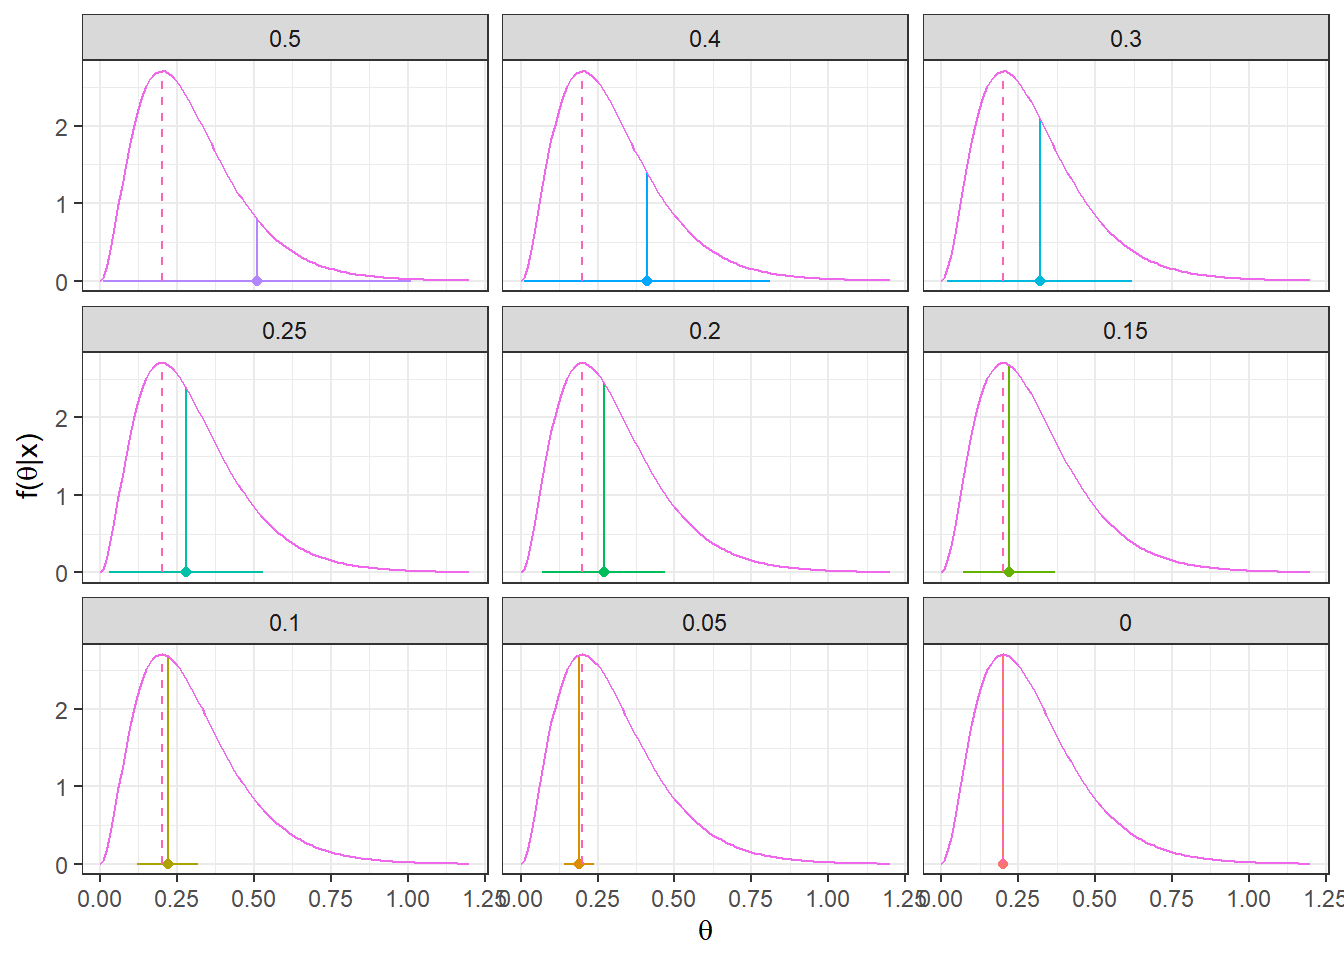
\includegraphics[width=0.8\linewidth]{InfBayes_files/figure-latex/unnamed-chunk-19-1} \end{center}

Como comentado no resultado anterior, quando \(\varepsilon \downarrow 0\), temos que \({\delta}^*(\boldsymbol x)=Moda(\theta|\boldsymbol x)\) \(= \displaystyle\sup_{\theta} f(\theta|\boldsymbol x)\).

\(\dfrac{\partial f(\theta|\boldsymbol x)}{\partial \theta}\) \(=(A_x-B_x\theta)\theta^{A_x-1}e^{-B_x\theta}=0\) \(\Leftrightarrow \theta =\dfrac{A_x}{B_x}\)

\({\delta}^*(\boldsymbol X) = Moda(\theta|\boldsymbol X)\) \(=\dfrac{a+\sum X_i-1}{b+n}\) \(=\dfrac{b}{b+n}\left(\dfrac{a-1}{b}\right)+\dfrac{n}{b+n}~\bar{X}\).

\(~\)

\textbf{Resultado.} Seja \(L(d,\theta)=c_1(d-\theta)~\mathbb{I}(d\geq \theta)+c_2(\theta-d)~\mathbb{I}(d<\theta)\) com \(c_1>0\), \(c_2 >0\). Então, \({\delta}^*(\boldsymbol{x})\) é tal que \(P\left(\theta\leq {\delta}^*(\boldsymbol{x})\big|\boldsymbol x\right)=\dfrac{c_1}{c_1+c_2}\). Em particular, se \(c_1=c_2=c\), temos a \emph{perda absoluta} \(L(d,\theta)=c~|d-\theta|\) e \({\delta}^*(\boldsymbol{X})=Med(\theta|\boldsymbol X)\).

\textbf{Demo:} exercício.

\(~\)

\(~\)

\hypertarget{estimauxe7uxe3o-por-regiuxf5es}{%
\section{Estimação por Regiões}\label{estimauxe7uxe3o-por-regiuxf5es}}

Em um problema de estimação por regiões (ou estimação intervalar, no caso univariado), o objetivo é obter um conjunto de valores razoáveis para \(\theta\). Mais formalmente, temos um problema aonde a decisão consiste em escolher um subconjunto do espaço paramétrico, de modo que \(\mathcal{D}=\mathcal{A}\), onde \(\mathcal{A}\) é \(\sigma\)-algebra de subconjuntos de \(\Theta\). Uma estimativa por região é comumente chamada na literatura Bayesiana de \textbf{região de credibilidade} (\textbf{intervalo de credibilidade}, no caso univariado) ou \textbf{região de probabilidade} \(~\gamma=1-\alpha\).

\(~\)

\textbf{Exemplo 1.} Suponha que a distribuição a posteriori é \(f(\theta|\boldsymbol{x})=4\theta~\mathbb{I}_{[0,1/2)}(\theta)+4(1-\theta)~\mathbb{I}_{[1/2,1]}(\theta)\). Uma possível estimativa intervalar é um intervalo central ou um intervalo simétrico em torno da média (ou da moda) com uma probabilidade \(\gamma = 1-\alpha\). Nesse caso, vamos considerar um intervalo central no sentido que deixa de fora conjuntos caudais de probabilidade \(\alpha/2\). Note que é possível obter o intervalo de forma analítica nesse exemplo. A seguir, são apresentadas as funções de distribuição \(F\) e quantílica \(Q\) a posteriori e o intervalo de credibilidade \(\alpha\).

\(F(\theta|\boldsymbol x)\) \(=\displaystyle \int_0^\theta f(t|x)dt\)
\(=\displaystyle \int_0^\theta\left[4t~\mathbb I_{[0,1/2]}(t)+(4-4t)~\mathbb I_{(1/2,1]}(t)\right]dt\)
\(=\left\{\begin{array}{lcc} 2\theta^2 &,& \theta\leq 1/2\\ -2\theta^2+4\theta-1 &,& \theta>1/2\end{array}\right.\)

\(Q(p)=\left\{\begin{array}{lcc} \sqrt{\dfrac{p}{2}} &,& p\leq 1/2\\ 1-\sqrt{\dfrac{1-p}{2}} &,& p>1/2\end{array}\right.\)

\(I.C.(1-\alpha)=\left[\sqrt{\dfrac{\alpha/2}{2}};1-\sqrt{\dfrac{\alpha/2}{2}}\right]\).

\begin{Shaded}
\begin{Highlighting}[]
\NormalTok{alpha=}\FloatTok{0.1}
\NormalTok{theta =}\StringTok{ }\KeywordTok{seq}\NormalTok{(}\DecValTok{0}\NormalTok{,}\DecValTok{1}\NormalTok{,}\FloatTok{0.01}\NormalTok{)}
\CommentTok{# Densidade a posteriori}
\NormalTok{dpost =}\StringTok{ }\KeywordTok{Vectorize}\NormalTok{(}\ControlFlowTok{function}\NormalTok{(t)\{ }\DecValTok{4}\OperatorTok{*}\NormalTok{t}\OperatorTok{*}\KeywordTok{I}\NormalTok{(t}\OperatorTok{>=}\DecValTok{0}\NormalTok{)}\OperatorTok{*}\KeywordTok{I}\NormalTok{(t}\OperatorTok{<=}\FloatTok{0.5}\NormalTok{)}\OperatorTok{+}
\StringTok{    }\DecValTok{4}\OperatorTok{*}\NormalTok{(}\DecValTok{1}\OperatorTok{-}\NormalTok{t)}\OperatorTok{*}\KeywordTok{I}\NormalTok{(t}\OperatorTok{>}\FloatTok{0.5}\NormalTok{)}\OperatorTok{*}\KeywordTok{I}\NormalTok{(t}\OperatorTok{<=}\DecValTok{1}\NormalTok{) \})}
\CommentTok{# F. Distribuição a posteriori}
\NormalTok{ppost =}\StringTok{ }\KeywordTok{Vectorize}\NormalTok{(}\ControlFlowTok{function}\NormalTok{(t)\{ }\DecValTok{2}\OperatorTok{*}\NormalTok{(t}\OperatorTok{^}\DecValTok{2}\NormalTok{)}\OperatorTok{*}\KeywordTok{I}\NormalTok{(t}\OperatorTok{>=}\DecValTok{0}\NormalTok{)}\OperatorTok{*}\KeywordTok{I}\NormalTok{(t}\OperatorTok{<=}\FloatTok{0.5}\NormalTok{)}\OperatorTok{+}
\StringTok{    }\DecValTok{4}\OperatorTok{*}\NormalTok{(}\DecValTok{1}\OperatorTok{-}\NormalTok{t)}\OperatorTok{*}\KeywordTok{I}\NormalTok{(t}\OperatorTok{>}\FloatTok{0.5}\NormalTok{)}\OperatorTok{*}\KeywordTok{I}\NormalTok{(t}\OperatorTok{<=}\DecValTok{1}\NormalTok{)}\OperatorTok{+}\KeywordTok{I}\NormalTok{(t}\OperatorTok{>}\DecValTok{1}\NormalTok{) \})}
\CommentTok{# F. Quantílica a posteriori}
\NormalTok{qpost =}\StringTok{ }\KeywordTok{Vectorize}\NormalTok{(}\ControlFlowTok{function}\NormalTok{(t)\{ }\KeywordTok{ifelse}\NormalTok{(t}\OperatorTok{<=}\FloatTok{0.5}\NormalTok{, }\KeywordTok{sqrt}\NormalTok{(t}\OperatorTok{/}\DecValTok{2}\NormalTok{)}\OperatorTok{*}\KeywordTok{I}\NormalTok{(t}\OperatorTok{>}\DecValTok{0}\NormalTok{),}
\NormalTok{    (}\DecValTok{1}\OperatorTok{-}\KeywordTok{sqrt}\NormalTok{((}\DecValTok{1}\OperatorTok{-}\NormalTok{t)}\OperatorTok{/}\DecValTok{2}\NormalTok{))}\OperatorTok{*}\KeywordTok{I}\NormalTok{(t}\OperatorTok{<}\DecValTok{1}\NormalTok{)}\OperatorTok{+}\KeywordTok{I}\NormalTok{(t}\OperatorTok{>=}\DecValTok{1}\NormalTok{)) \})}
\NormalTok{post =}\StringTok{ }\KeywordTok{dpost}\NormalTok{(theta)}
\NormalTok{l =}\StringTok{ }\KeywordTok{c}\NormalTok{(}\KeywordTok{qpost}\NormalTok{((alpha}\OperatorTok{/}\DecValTok{2}\NormalTok{)),}\KeywordTok{qpost}\NormalTok{((}\DecValTok{1}\OperatorTok{-}\NormalTok{alpha}\OperatorTok{/}\DecValTok{2}\NormalTok{)))}
\NormalTok{X =}\StringTok{ }\KeywordTok{tibble}\NormalTok{(}\DataTypeTok{theta=}\NormalTok{theta,}\DataTypeTok{Posterior=}\NormalTok{post)}
\KeywordTok{ggplot}\NormalTok{(}\DataTypeTok{data=}\NormalTok{X,}\DataTypeTok{mapping =} \KeywordTok{aes}\NormalTok{(}\DataTypeTok{x=}\NormalTok{theta,}\DataTypeTok{y=}\NormalTok{Posterior)) }\OperatorTok{+}
\StringTok{  }\KeywordTok{geom_line}\NormalTok{(}\DataTypeTok{lwd=}\FloatTok{1.5}\NormalTok{) }\OperatorTok{+}
\StringTok{  }\KeywordTok{geom_area}\NormalTok{(}\DataTypeTok{data=}\KeywordTok{subset}\NormalTok{(X, theta }\OperatorTok{>=}\StringTok{ }\NormalTok{l[}\DecValTok{1}\NormalTok{] }\OperatorTok{&}\StringTok{ }\NormalTok{theta }\OperatorTok{<=}\StringTok{ }\NormalTok{l[}\DecValTok{2}\NormalTok{]),}\DataTypeTok{fill =} \StringTok{"blue"}\NormalTok{, }\DataTypeTok{alpha=}\FloatTok{0.5}\NormalTok{)}\OperatorTok{+}
\StringTok{  }\KeywordTok{theme_bw}\NormalTok{()}
\end{Highlighting}
\end{Shaded}

\begin{center}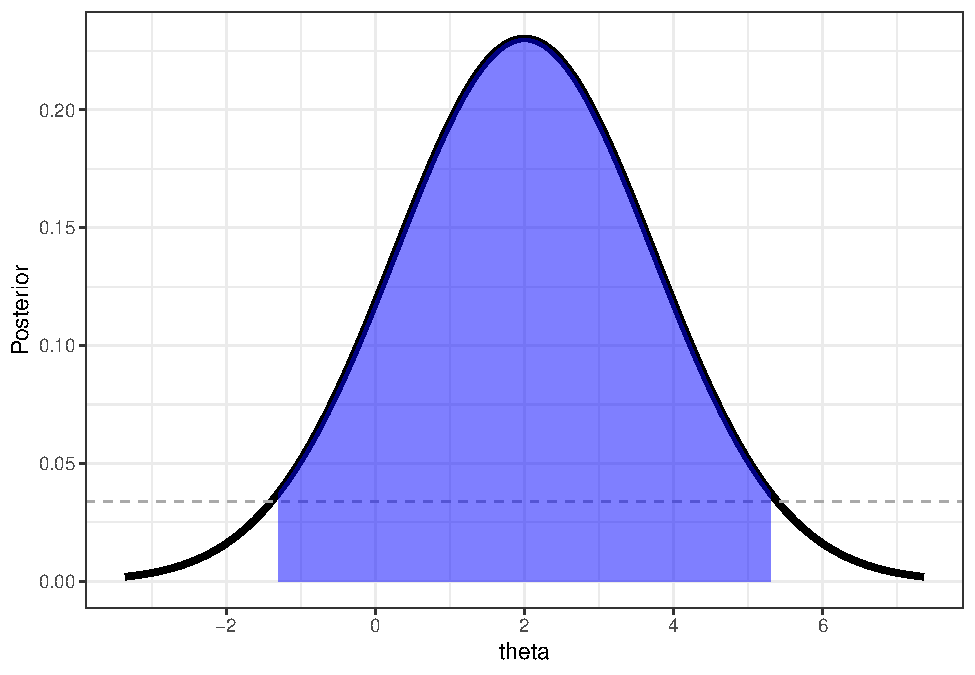
\includegraphics[width=0.8\linewidth]{InfBayes_files/figure-latex/unnamed-chunk-21-1} \end{center}

\(~\)

\textbf{Exemplo 2.} Por fim, suponha que a distribuição a posteriori é \(f(\theta|\boldsymbol{x})=(2-4\theta)~\mathbb{I}_{[0,1/2)}(\theta)+(4\theta-2)~\mathbb{I}_{[1/2,1]}(\theta)\). Vamos construir um intervalo como no Exemplo anterior.

\(F(\theta|\boldsymbol x)\) \(=\left\{\begin{array}{lcc} 2\theta(1-\theta) &,& \theta\leq 1/2\\ 2\theta(\theta-1)+1 &,& \theta>1/2\end{array}\right.\)

\(Q(p)=\left\{\begin{array}{lcc} \dfrac{1}{2}-\dfrac{\sqrt{1-2p}}{2} &,& p\leq 1/2\\ \dfrac{1}{2}+\dfrac{\sqrt{2p-1}}{2} &,& p>1/2\end{array}\right.\)

\(I.C.(1-\alpha)=\left[\dfrac{1}{2}-\dfrac{\sqrt{1-\alpha}}{2};\dfrac{1}{2}+\dfrac{\sqrt{1-\alpha}}{2}\right]\).

\begin{Shaded}
\begin{Highlighting}[]
\NormalTok{alpha=}\FloatTok{0.1}
\NormalTok{theta =}\StringTok{ }\KeywordTok{seq}\NormalTok{(}\DecValTok{0}\NormalTok{,}\DecValTok{1}\NormalTok{,}\FloatTok{0.01}\NormalTok{)}
\CommentTok{# Densidade a posteriori}
\NormalTok{dpost =}\StringTok{ }\KeywordTok{Vectorize}\NormalTok{(}\ControlFlowTok{function}\NormalTok{(t)\{ (}\DecValTok{2-4}\OperatorTok{*}\NormalTok{t)}\OperatorTok{*}\KeywordTok{I}\NormalTok{(t}\OperatorTok{>=}\DecValTok{0}\NormalTok{)}\OperatorTok{*}\KeywordTok{I}\NormalTok{(t}\OperatorTok{<=}\FloatTok{0.5}\NormalTok{)}\OperatorTok{+}
\StringTok{    }\NormalTok{(}\DecValTok{4}\OperatorTok{*}\NormalTok{t}\DecValTok{-2}\NormalTok{)}\OperatorTok{*}\KeywordTok{I}\NormalTok{(t}\OperatorTok{>}\FloatTok{0.5}\NormalTok{)}\OperatorTok{*}\KeywordTok{I}\NormalTok{(t}\OperatorTok{<=}\DecValTok{1}\NormalTok{) \})}
\CommentTok{# F. Distribuição a posteriori}
\NormalTok{ppost =}\StringTok{ }\KeywordTok{Vectorize}\NormalTok{(}\ControlFlowTok{function}\NormalTok{(t)\{ }\DecValTok{2}\OperatorTok{*}\NormalTok{t}\OperatorTok{*}\NormalTok{(}\DecValTok{1}\OperatorTok{-}\NormalTok{t)}\OperatorTok{*}\KeywordTok{I}\NormalTok{(t}\OperatorTok{>=}\DecValTok{0}\NormalTok{)}\OperatorTok{*}\KeywordTok{I}\NormalTok{(t}\OperatorTok{<=}\FloatTok{0.5}\NormalTok{)}\OperatorTok{+}
\StringTok{    }\NormalTok{(}\DecValTok{2}\OperatorTok{*}\NormalTok{(t}\OperatorTok{^}\DecValTok{2}\NormalTok{)}\OperatorTok{-}\DecValTok{2}\OperatorTok{*}\NormalTok{t}\OperatorTok{+}\DecValTok{1}\NormalTok{)}\OperatorTok{*}\KeywordTok{I}\NormalTok{(t}\OperatorTok{>}\FloatTok{0.5}\NormalTok{)}\OperatorTok{*}\KeywordTok{I}\NormalTok{(t}\OperatorTok{<=}\DecValTok{1}\NormalTok{)}\OperatorTok{+}\KeywordTok{I}\NormalTok{(t}\OperatorTok{>}\DecValTok{1}\NormalTok{) \})}
\CommentTok{# F. Quantílica a posteriori}
\NormalTok{qpost =}\StringTok{ }\KeywordTok{Vectorize}\NormalTok{(}\ControlFlowTok{function}\NormalTok{(t)\{ }\KeywordTok{ifelse}\NormalTok{(t}\OperatorTok{<=}\FloatTok{0.5}\NormalTok{, (}\FloatTok{0.5}\OperatorTok{-}\KeywordTok{sqrt}\NormalTok{(}\DecValTok{1-2}\OperatorTok{*}\NormalTok{t)}\OperatorTok{/}\DecValTok{2}\NormalTok{)}\OperatorTok{*}\KeywordTok{I}\NormalTok{(t}\OperatorTok{>}\DecValTok{0}\NormalTok{),}
\NormalTok{    (}\FloatTok{0.5}\OperatorTok{+}\KeywordTok{sqrt}\NormalTok{(}\DecValTok{2}\OperatorTok{*}\NormalTok{t}\DecValTok{-1}\NormalTok{)}\OperatorTok{/}\DecValTok{2}\NormalTok{)}\OperatorTok{*}\KeywordTok{I}\NormalTok{(t}\OperatorTok{<}\DecValTok{1}\NormalTok{)}\OperatorTok{+}\KeywordTok{I}\NormalTok{(t}\OperatorTok{>=}\DecValTok{1}\NormalTok{)) \})}
\NormalTok{post =}\StringTok{ }\KeywordTok{dpost}\NormalTok{(theta)}
\NormalTok{l =}\StringTok{ }\KeywordTok{c}\NormalTok{(}\KeywordTok{qpost}\NormalTok{((alpha}\OperatorTok{/}\DecValTok{2}\NormalTok{)),}\KeywordTok{qpost}\NormalTok{((}\DecValTok{1}\OperatorTok{-}\NormalTok{alpha}\OperatorTok{/}\DecValTok{2}\NormalTok{)))}
\NormalTok{X =}\StringTok{ }\KeywordTok{tibble}\NormalTok{(}\DataTypeTok{theta=}\NormalTok{theta,}\DataTypeTok{Posterior=}\NormalTok{post)}
\KeywordTok{ggplot}\NormalTok{(}\DataTypeTok{data=}\NormalTok{X,}\DataTypeTok{mapping =} \KeywordTok{aes}\NormalTok{(}\DataTypeTok{x=}\NormalTok{theta,}\DataTypeTok{y=}\NormalTok{Posterior)) }\OperatorTok{+}
\StringTok{  }\KeywordTok{geom_line}\NormalTok{(}\DataTypeTok{lwd=}\FloatTok{1.5}\NormalTok{) }\OperatorTok{+}
\StringTok{  }\KeywordTok{geom_area}\NormalTok{(}\DataTypeTok{data=}\KeywordTok{subset}\NormalTok{(X, theta }\OperatorTok{>=}\StringTok{ }\NormalTok{l[}\DecValTok{1}\NormalTok{] }\OperatorTok{&}\StringTok{ }\NormalTok{theta }\OperatorTok{<=}\StringTok{ }\NormalTok{l[}\DecValTok{2}\NormalTok{]),}\DataTypeTok{fill =} \StringTok{"blue"}\NormalTok{, }\DataTypeTok{alpha=}\FloatTok{0.5}\NormalTok{)}\OperatorTok{+}
\StringTok{  }\KeywordTok{theme_bw}\NormalTok{()}
\end{Highlighting}
\end{Shaded}

\begin{center}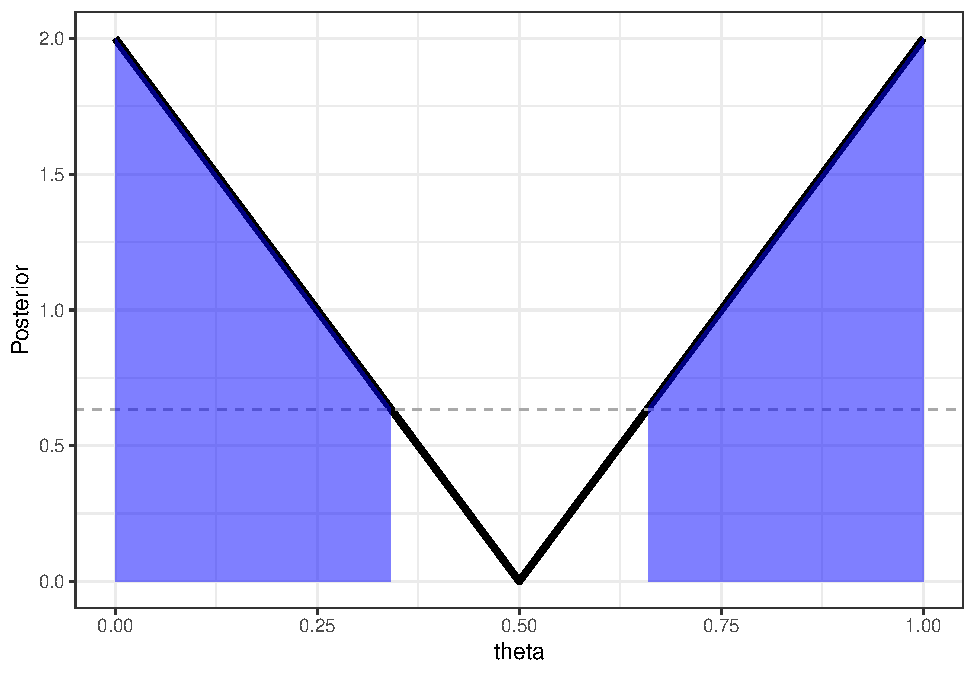
\includegraphics[width=0.8\linewidth]{InfBayes_files/figure-latex/unnamed-chunk-22-1} \end{center}

Note que, nesse exemplo, as regiões que tem mais densidade a posteriori foram excluídas do intervalo. Isso não faz muito sentido pois essas regiões têm maior chance de conter o \(\theta\) que quaquer outra região de mesmo tamanho.

\(~\)

\(~\)

Uma \emph{função de perda} razoável para um problema de estimação por região deve levar em consideração dois fatores:

\begin{itemize}
\item
  O tamanho da região \(d \in \mathcal{A}\) (deseja-se uma região que seja menor que o espaço paramétrico);
\item
  Pertinência de \(\theta\) na região \(d\).
\end{itemize}

Assim, considere uma função de perda da forma

\(L(d,\theta)=\lambda(d)-k~\mathbb I_d(\theta)\),

onde \(\lambda(d)\) é o ``tamanho'' da região \(d\). Por exemplo, a medida de Lebesgue, no caso contínuo, ou a medida de contagem, no caso discreto (no caso geral, considere uma medida que domina a distribuição a posteriori, \(P(\theta|\boldsymbol x) \ll \lambda\)). No caso absolutamente contínuo, o risco a posteriori de uma decisão \(d \in \mathcal{A}\) é

\({r}_{x}(d)\) \(=\displaystyle\int_\Theta \left[\lambda(d)-k~\mathbb I_d(\theta)\right]dP(\theta|\boldsymbol x)\) \(=\displaystyle \int_\Theta\mathbb I_d(\theta)d\theta-\int_\Theta k~\mathbb I_d(\theta)f(\theta|\boldsymbol x)d\theta\) \(=\displaystyle \int_d\left(1-kf(\theta|\boldsymbol x)\right)d\theta\).

Esse risco é mínimo quando \(d=\left\{\theta\in\Theta:1-kf(\theta|\boldsymbol x)\leq 0\right\}\) \(\Leftrightarrow d=\{\theta\in\Theta:f(\theta|\boldsymbol x)\geq 1/k\}\).

Assim, a decisão de Bayes contra essa função de perda consiste em escolher uma região \(d \in \mathcal{A}\) que contêm os pontos do espaço paramétrico com maior densidade a posteriori.

\(~\)

\textbf{Definição:} A região \(R\subseteq \Theta\) é dita ser uma região HPD (Highest Posterior Density) de probabilidade \(\gamma\) se

\begin{enumerate}
\def\labelenumi{\roman{enumi}.}
\item
  \(P(\theta\in R|\boldsymbol x)=\gamma\);
\item
  \(\forall \theta \in R\) e \(\forall \theta^\prime\notin R\), \(f(\theta|\boldsymbol x)\geq f(\theta^\prime|\boldsymbol x)\).
\end{enumerate}

\(~\)

\textbf{Voltando ao Exemplo 2.} As regiões centrais nesse exemplo tem menor densidade a posteriori. Assim, uma região HPD de probabilidade \(\gamma=1-\alpha\) é dada por

\(I.C.(1-\alpha)=\left[0~;~\dfrac{1}{2}-\dfrac{\sqrt{\alpha}}{2}\right]\bigcup \left[\dfrac{1}{2}+\dfrac{\sqrt{\alpha}}{2}~;~1\right]\)

\begin{Shaded}
\begin{Highlighting}[]
\NormalTok{alpha=}\FloatTok{0.1}
\NormalTok{theta =}\StringTok{ }\KeywordTok{seq}\NormalTok{(}\DecValTok{0}\NormalTok{,}\DecValTok{1}\NormalTok{,}\FloatTok{0.01}\NormalTok{)}
\CommentTok{# Densidade a posteriori}
\NormalTok{dpost =}\StringTok{ }\KeywordTok{Vectorize}\NormalTok{(}\ControlFlowTok{function}\NormalTok{(t)\{ (}\DecValTok{2-4}\OperatorTok{*}\NormalTok{t)}\OperatorTok{*}\KeywordTok{I}\NormalTok{(t}\OperatorTok{>=}\DecValTok{0}\NormalTok{)}\OperatorTok{*}\KeywordTok{I}\NormalTok{(t}\OperatorTok{<=}\FloatTok{0.5}\NormalTok{)}\OperatorTok{+}
\StringTok{    }\NormalTok{(}\DecValTok{4}\OperatorTok{*}\NormalTok{t}\DecValTok{-2}\NormalTok{)}\OperatorTok{*}\KeywordTok{I}\NormalTok{(t}\OperatorTok{>}\FloatTok{0.5}\NormalTok{)}\OperatorTok{*}\KeywordTok{I}\NormalTok{(t}\OperatorTok{<=}\DecValTok{1}\NormalTok{) \})}
\CommentTok{# F. Distribuição a posteriori}
\NormalTok{ppost =}\StringTok{ }\KeywordTok{Vectorize}\NormalTok{(}\ControlFlowTok{function}\NormalTok{(t)\{ }\DecValTok{2}\OperatorTok{*}\NormalTok{t}\OperatorTok{*}\NormalTok{(}\DecValTok{1}\OperatorTok{-}\NormalTok{t)}\OperatorTok{*}\KeywordTok{I}\NormalTok{(t}\OperatorTok{>=}\DecValTok{0}\NormalTok{)}\OperatorTok{*}\KeywordTok{I}\NormalTok{(t}\OperatorTok{<=}\FloatTok{0.5}\NormalTok{)}\OperatorTok{+}
\StringTok{    }\NormalTok{(}\DecValTok{2}\OperatorTok{*}\NormalTok{(t}\OperatorTok{^}\DecValTok{2}\NormalTok{)}\OperatorTok{-}\DecValTok{2}\OperatorTok{*}\NormalTok{t}\OperatorTok{+}\DecValTok{1}\NormalTok{)}\OperatorTok{*}\KeywordTok{I}\NormalTok{(t}\OperatorTok{>}\FloatTok{0.5}\NormalTok{)}\OperatorTok{*}\KeywordTok{I}\NormalTok{(t}\OperatorTok{<=}\DecValTok{1}\NormalTok{)}\OperatorTok{+}\KeywordTok{I}\NormalTok{(t}\OperatorTok{>}\DecValTok{1}\NormalTok{) \})}
\CommentTok{# F. Quantílica a posteriori}
\NormalTok{qpost =}\StringTok{ }\KeywordTok{Vectorize}\NormalTok{(}\ControlFlowTok{function}\NormalTok{(t)\{ }\KeywordTok{ifelse}\NormalTok{(t}\OperatorTok{<=}\FloatTok{0.5}\NormalTok{, (}\FloatTok{0.5}\OperatorTok{-}\KeywordTok{sqrt}\NormalTok{(}\DecValTok{1-2}\OperatorTok{*}\NormalTok{t)}\OperatorTok{/}\DecValTok{2}\NormalTok{)}\OperatorTok{*}\KeywordTok{I}\NormalTok{(t}\OperatorTok{>}\DecValTok{0}\NormalTok{),}
\NormalTok{    (}\FloatTok{0.5}\OperatorTok{+}\KeywordTok{sqrt}\NormalTok{(}\DecValTok{2}\OperatorTok{*}\NormalTok{t}\DecValTok{-1}\NormalTok{)}\OperatorTok{/}\DecValTok{2}\NormalTok{)}\OperatorTok{*}\KeywordTok{I}\NormalTok{(t}\OperatorTok{<}\DecValTok{1}\NormalTok{)}\OperatorTok{+}\KeywordTok{I}\NormalTok{(t}\OperatorTok{>=}\DecValTok{1}\NormalTok{)) \})}
\NormalTok{post =}\StringTok{ }\KeywordTok{dpost}\NormalTok{(theta)}
\NormalTok{l =}\StringTok{ }\KeywordTok{c}\NormalTok{(}\KeywordTok{qpost}\NormalTok{((}\DecValTok{1}\OperatorTok{-}\NormalTok{alpha)}\OperatorTok{/}\DecValTok{2}\NormalTok{),}\KeywordTok{qpost}\NormalTok{((alpha}\OperatorTok{+}\DecValTok{1}\NormalTok{)}\OperatorTok{/}\DecValTok{2}\NormalTok{))}
\NormalTok{X =}\StringTok{ }\KeywordTok{tibble}\NormalTok{(}\DataTypeTok{theta=}\NormalTok{theta,}\DataTypeTok{Posterior=}\NormalTok{post)}
\KeywordTok{ggplot}\NormalTok{(}\DataTypeTok{data=}\NormalTok{X,}\DataTypeTok{mapping =} \KeywordTok{aes}\NormalTok{(}\DataTypeTok{x=}\NormalTok{theta,}\DataTypeTok{y=}\NormalTok{Posterior)) }\OperatorTok{+}
\StringTok{  }\KeywordTok{geom_line}\NormalTok{(}\DataTypeTok{lwd=}\FloatTok{1.5}\NormalTok{) }\OperatorTok{+}
\StringTok{  }\KeywordTok{geom_hline}\NormalTok{(}\DataTypeTok{yintercept=}\KeywordTok{dpost}\NormalTok{(l[}\DecValTok{1}\NormalTok{]), }\DataTypeTok{lty=}\DecValTok{2}\NormalTok{, }\DataTypeTok{col=}\StringTok{"darkgray"}\NormalTok{) }\OperatorTok{+}
\StringTok{  }\KeywordTok{geom_area}\NormalTok{(}\DataTypeTok{data=}\KeywordTok{subset}\NormalTok{(X, theta }\OperatorTok{<=}\StringTok{ }\NormalTok{l[}\DecValTok{1}\NormalTok{]),}\DataTypeTok{fill =} \StringTok{"blue"}\NormalTok{, }\DataTypeTok{alpha=}\FloatTok{0.5}\NormalTok{) }\OperatorTok{+}
\StringTok{  }\KeywordTok{geom_area}\NormalTok{(}\DataTypeTok{data=}\KeywordTok{subset}\NormalTok{(X, theta }\OperatorTok{>=}\StringTok{ }\NormalTok{l[}\DecValTok{2}\NormalTok{]),}\DataTypeTok{fill =} \StringTok{"blue"}\NormalTok{, }\DataTypeTok{alpha=}\FloatTok{0.5}\NormalTok{)}\OperatorTok{+}
\StringTok{  }\KeywordTok{theme_bw}\NormalTok{()}
\end{Highlighting}
\end{Shaded}

\begin{center}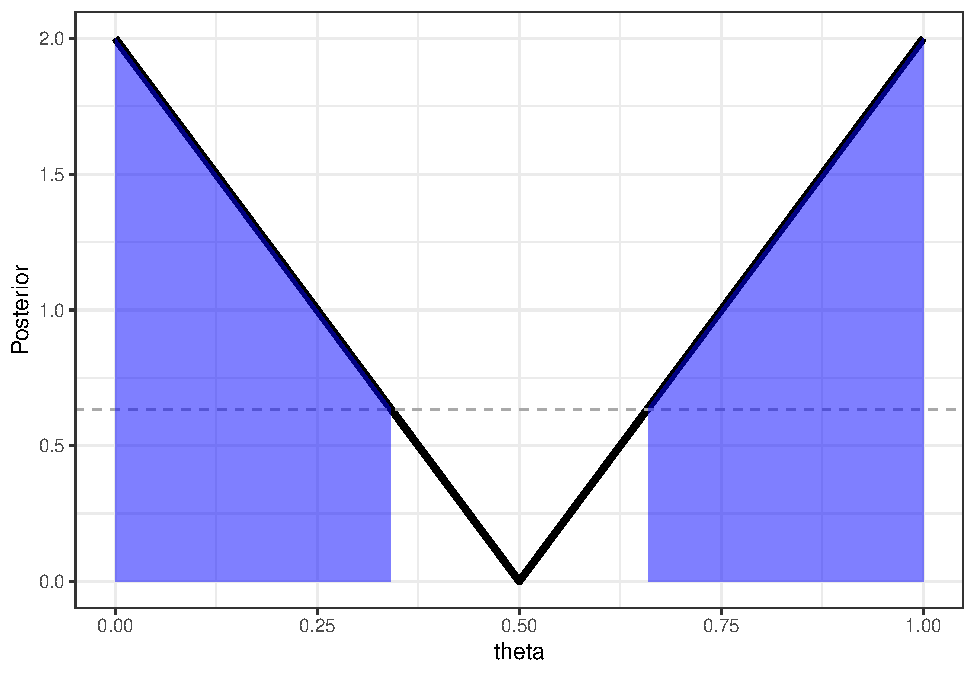
\includegraphics[width=0.8\linewidth]{InfBayes_files/figure-latex/unnamed-chunk-23-1} \end{center}

Note que na solução anterior, o comprimento do intervalo era \(\sqrt{1-\alpha}\), enquanto que o comprimento do HPD é \(1-\sqrt{\alpha}\). Tomando, por exemplo, \(\alpha=0.1\) temos que \(\sqrt{1-\alpha} \approx 0.95\) enquanto \(1-\sqrt{\alpha}\approx 0.68\). Por conter apenas os pontos com maior densidade, o HPD sempre terá comprimento menor ou igual a qualquer intervalo com mesma probabilidade.

\(~\)

\textbf{Exemplo 3.} Considere \(X_1,...,X_n\) c.i.i.d. tais que \(X_i|\theta\sim N(\theta,1/\tau)\) , \(\tau=1/\sigma^2\) , com \(\tau\) conhecido (fixado). Vimos que se, a priori, \(\theta\sim N(m,1/v)\) então \(\theta|\boldsymbol x\sim N\left(\underbrace{\dfrac{vm+n\tau\bar x}{v+n\tau}}_{M_x},\underbrace{\dfrac{1}{v+n\tau}}_{V_x}\right)\) e, assim, \(Z=\dfrac{\theta-M_x}{\sqrt V_x}~\Bigg|~\boldsymbol x\sim N(0,1)\).

O intervalo HPD de probabilidade \(\gamma=1-\alpha=0.95\) é

\(I.C.(1-\alpha)=\) \(\left[M-z_{\alpha/2}\sqrt V;M+z_{\alpha/2}\sqrt V\right]\) \(=\left[\dfrac{vm+n\tau\bar x}{v+n\tau}\pm1.96\sqrt{\dfrac{1}{v+n\tau}}\right]\).

Uma possível forma de representar falta de informação a priori é tomar o limite \(~v\downarrow 0~~\) (\(1/v\uparrow \infty\)). Dessa forma, tem-se

\(\theta|\boldsymbol x\sim N(\bar x,1/(n\tau))\sim N(\bar x,\sigma^2/n)\),

e o intervalo HPD coincide com o I.C. frequentista

\(I.C.(1-\alpha)=\left[\bar x\pm 1.96\dfrac{\sigma}{\sqrt{n}}\right]\).

\begin{Shaded}
\begin{Highlighting}[]
\NormalTok{mx=}\DecValTok{2}\NormalTok{; vx=}\KeywordTok{sqrt}\NormalTok{(}\DecValTok{3}\NormalTok{)}
\NormalTok{alpha=}\FloatTok{0.05}
\NormalTok{theta =}\StringTok{ }\KeywordTok{seq}\NormalTok{(}\KeywordTok{qnorm}\NormalTok{(}\FloatTok{0.001}\NormalTok{,mx,vx),}\KeywordTok{qnorm}\NormalTok{(}\FloatTok{0.999}\NormalTok{,mx,vx),}\DataTypeTok{length.out=}\DecValTok{100}\NormalTok{)}
\NormalTok{post =}\StringTok{ }\KeywordTok{dnorm}\NormalTok{(theta,mx,vx)}
\NormalTok{l =}\StringTok{ }\KeywordTok{c}\NormalTok{(}\KeywordTok{qnorm}\NormalTok{(alpha}\OperatorTok{/}\DecValTok{2}\NormalTok{,mx,vx),}\KeywordTok{qnorm}\NormalTok{(}\DecValTok{1}\OperatorTok{-}\NormalTok{alpha}\OperatorTok{/}\DecValTok{2}\NormalTok{,mx,vx))}
\NormalTok{X =}\StringTok{ }\KeywordTok{tibble}\NormalTok{(}\DataTypeTok{theta=}\NormalTok{theta,}\DataTypeTok{Posterior=}\NormalTok{post)}
\KeywordTok{ggplot}\NormalTok{(}\DataTypeTok{data=}\NormalTok{X,}\DataTypeTok{mapping =} \KeywordTok{aes}\NormalTok{(}\DataTypeTok{x=}\NormalTok{theta,}\DataTypeTok{y=}\NormalTok{Posterior)) }\OperatorTok{+}
\StringTok{  }\KeywordTok{geom_line}\NormalTok{(}\DataTypeTok{lwd=}\FloatTok{1.5}\NormalTok{) }\OperatorTok{+}
\StringTok{  }\KeywordTok{geom_hline}\NormalTok{(}\DataTypeTok{yintercept=}\KeywordTok{dnorm}\NormalTok{(l[}\DecValTok{1}\NormalTok{],mx,vx), }\DataTypeTok{lty=}\DecValTok{2}\NormalTok{, }\DataTypeTok{col=}\StringTok{"darkgray"}\NormalTok{) }\OperatorTok{+}
\StringTok{  }\KeywordTok{geom_area}\NormalTok{(}\DataTypeTok{data=}\KeywordTok{subset}\NormalTok{(X, theta }\OperatorTok{>=}\StringTok{ }\NormalTok{l[}\DecValTok{1}\NormalTok{] }\OperatorTok{&}\StringTok{ }\NormalTok{theta }\OperatorTok{<=}\StringTok{ }\NormalTok{l[}\DecValTok{2}\NormalTok{]),}\DataTypeTok{fill =} \StringTok{"blue"}\NormalTok{, }\DataTypeTok{alpha=}\FloatTok{0.5}\NormalTok{)}\OperatorTok{+}
\StringTok{  }\KeywordTok{theme_bw}\NormalTok{()}
\end{Highlighting}
\end{Shaded}

\begin{center}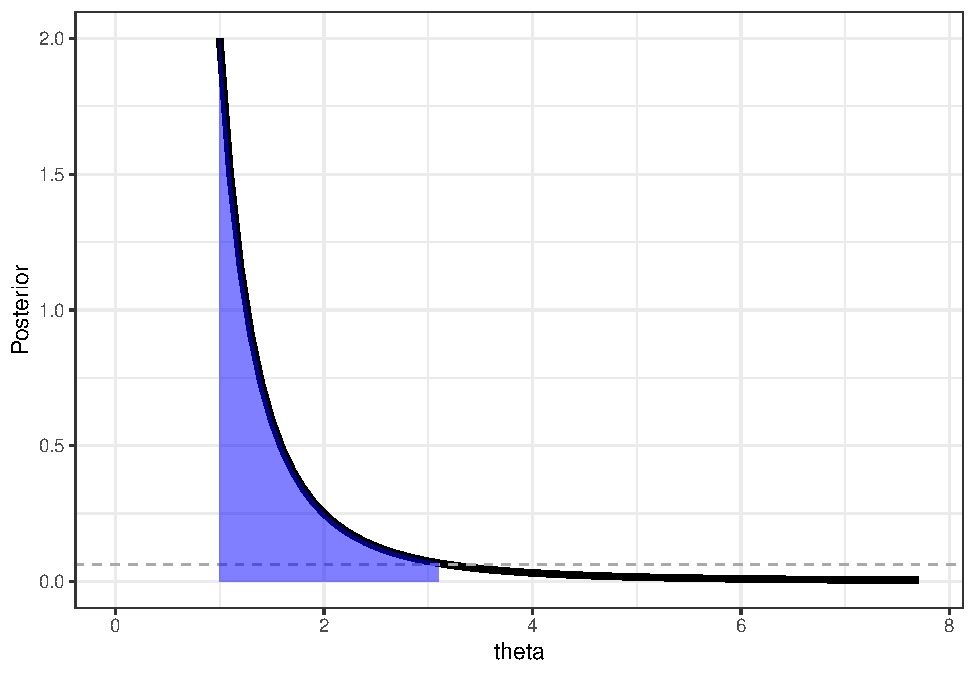
\includegraphics[width=0.8\linewidth]{InfBayes_files/figure-latex/unnamed-chunk-24-1} \end{center}

\(~\)

\textbf{Exemplo 4:} Considere \(X_1,...,X_n\) c.i.i.d. tais que \(X_i|\theta\sim Unif(0,\theta)\). Vimos que se \(\theta\sim Pareto(a,b)\), então \(\theta|\boldsymbol x\sim Pareto (a+n,\max\{x_{(n)},b\})\)

\(f(\theta|\boldsymbol x) =\dfrac{(a+n)[\max\{x_{(n)},b\}]^{a+n}}{\theta^{a+n+1}}~\mathbb I_{[\max\{x_{(n)},b\},\infty)}\)

Note que a função de densidade a posteriori é estritamente decrescente de modo que o extremo inferior da região HPD é \(\max\{x_{(n)},b\}\). A função de distribuição a posteriori é

\(F(\theta|\boldsymbol x)=1-\left(\dfrac{\max\{x_{(n)},b\}}{\theta}\right)^{a+n}\),

de modo que o extremo superior do intervalo pode ser obtido fazendo

\(1-\left(\dfrac{\max\{x_{(n)},b\}}{\theta}\right)^{a+n}=\gamma\) \(\Leftrightarrow\dfrac{\max\{x_{(n)},b\}}{\theta^*}=(1-\gamma)^{1/(a+n)}\) \(\Leftrightarrow \theta^*=\dfrac{\max\{x_{(n)},b\}}{(1-\gamma)^{1/(a+n)}}\).

\(I.C.(1-\alpha)=\left[\max\{x_{(n)},b\},\dfrac{\max\{x_{(n)},b\}}{\alpha^{1/(a+n)}}\right]\)

\begin{Shaded}
\begin{Highlighting}[]
\NormalTok{ax=}\DecValTok{2}\NormalTok{; bx=}\DecValTok{1}
\NormalTok{maxt=bx}\OperatorTok{/}\NormalTok{((alpha}\OperatorTok{/}\DecValTok{3}\NormalTok{)}\OperatorTok{^}\NormalTok{(}\DecValTok{1}\OperatorTok{/}\NormalTok{ax))}
\NormalTok{alpha=}\FloatTok{0.1}
\NormalTok{limsup=bx}\OperatorTok{/}\NormalTok{(alpha}\OperatorTok{^}\NormalTok{(}\DecValTok{1}\OperatorTok{/}\NormalTok{ax))}
\NormalTok{theta =}\StringTok{ }\KeywordTok{seq}\NormalTok{(bx,maxt,}\FloatTok{0.1}\NormalTok{)}
\NormalTok{dpareto=}\KeywordTok{Vectorize}\NormalTok{(}\ControlFlowTok{function}\NormalTok{(t)\{}
\NormalTok{  ax}\OperatorTok{*}\NormalTok{(bx}\OperatorTok{^}\NormalTok{ax)}\OperatorTok{*}\KeywordTok{I}\NormalTok{(t}\OperatorTok{>=}\NormalTok{bx) }\OperatorTok{/}\StringTok{ }\NormalTok{(t}\OperatorTok{^}\NormalTok{(ax}\OperatorTok{+}\DecValTok{1}\NormalTok{)) \})}
\NormalTok{post =}\StringTok{ }\KeywordTok{dpareto}\NormalTok{(theta)}
\NormalTok{X =}\StringTok{ }\KeywordTok{tibble}\NormalTok{(}\DataTypeTok{theta=}\NormalTok{theta,}\DataTypeTok{Posterior=}\NormalTok{post)}
\KeywordTok{ggplot}\NormalTok{(}\DataTypeTok{data=}\NormalTok{X,}\DataTypeTok{mapping =} \KeywordTok{aes}\NormalTok{(}\DataTypeTok{x=}\NormalTok{theta,}\DataTypeTok{y=}\NormalTok{Posterior)) }\OperatorTok{+}
\StringTok{  }\KeywordTok{geom_line}\NormalTok{(}\DataTypeTok{lwd=}\FloatTok{1.5}\NormalTok{) }\OperatorTok{+}
\StringTok{  }\KeywordTok{xlim}\NormalTok{(}\KeywordTok{c}\NormalTok{(}\DecValTok{0}\NormalTok{,maxt))}\OperatorTok{+}
\StringTok{  }\KeywordTok{geom_hline}\NormalTok{(}\DataTypeTok{yintercept=}\KeywordTok{dpareto}\NormalTok{(limsup), }\DataTypeTok{lty=}\DecValTok{2}\NormalTok{, }\DataTypeTok{col=}\StringTok{"darkgray"}\NormalTok{) }\OperatorTok{+}
\StringTok{  }\KeywordTok{geom_area}\NormalTok{(}\DataTypeTok{data=}\KeywordTok{subset}\NormalTok{(X, theta }\OperatorTok{<=}\StringTok{ }\NormalTok{limsup),}\DataTypeTok{fill =} \StringTok{"blue"}\NormalTok{, }\DataTypeTok{alpha=}\FloatTok{0.5}\NormalTok{)}\OperatorTok{+}
\StringTok{  }\KeywordTok{theme_bw}\NormalTok{()}
\end{Highlighting}
\end{Shaded}

\begin{center}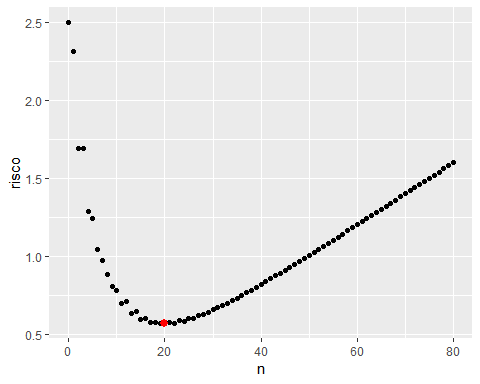
\includegraphics[width=0.8\linewidth]{InfBayes_files/figure-latex/unnamed-chunk-25-1} \end{center}

\(~\)

\(~\)

\hypertarget{custo-das-observauxe7uxf5es}{%
\section{Custo das Observações}\label{custo-das-observauxe7uxf5es}}

Suponha agora que o custo para observar uma amostra de tamanho \(n\) é dado por uma função custo \(c(n)\) e, antes de observar \(X_1,\ldots,X_n\), você precisa decidir qual o tamanho amostral ótimo, \(n^*\). Desta forma, considere a função de perda \(L(d,\theta,n) = L(d,\theta) + c(n)\) com risco

\(\rho_n(\delta,P)\) \(= E\left[L(d,\theta,n)\right]\) \(= E\left[L(d,\theta) + c(n)\right]\) \(= \rho_n(\delta,P) + c(n)\).

Note que (supostamente, por simplicidade) o custo \(c(n)\) não depende de \(\theta\). Se \(\delta^*\) é função de decisão de Bayes contra \(L(d,\theta)\) e a priori \(P\), o tamanho amostral ótimo \(n^*\) é o valor que minimiza

\(\rho_n(P)\) \(= \rho(\delta,P) + c(n)\) \(= \rho^*(P) + c(n)\).

\(~\)

\textbf{Exemplo.} Considere o exemplo visto anteriorimente em que \(\mathcal{D}=\{d_1,d_2\}\), \(\Theta=\{\theta_1,\theta_2\}=\{3/4,1/3\}\), \(P(\theta_1)=1/2\) e a função de perda é \(L(d,\theta)=10~\mathbb{I}(d_1,\theta_2) + 5~\mathbb{I}(d_2,\theta_1)\). Se \(X|\theta \sim Ber(\theta)\), a função de decisão de Bayes é \(\delta^*(x)=d_1~\mathbb{I}(x=1)+d_2~\mathbb{I}(x=0)\).

\(~\)

Suponha agora que é possível observar \(X_1,\ldots,X_n\) v.a. c.i.i.d. tais que \(X_i|\theta \sim Ber(\theta)\). Note que \(T(\boldsymbol X)=\sum X_i\) é suficiente para \(\theta\) com \(T(\boldsymbol X)|\theta \sim Bin(n,\theta)\) e

\(f(\theta_1|T(\boldsymbol X)=t)\)
\(=\dfrac{f(t|\theta_1)P(\theta_1)}{\displaystyle \sum_{i\in\{1,2\}} f(t|\theta_i)P(\theta_i)}\)
\(=\dfrac{f(t|\theta_1)}{\displaystyle \sum_{i\in\{1,2\}} f(t|\theta_i)}\)
\(=\dfrac{\binom{n}{t}\left(\frac{3}{4}\right)^t\left(\frac{1}{4}\right)^{n-t}}{\binom{n}{t}\left(\frac{3}{4}\right)^t\left(\frac{1}{4}\right)^{n-t}+\binom{n}{t}\left(\frac{1}{3}\right)^t\left(\frac{2}{3}\right)^{n-t}}\)
\(=\dfrac{1}{1+\left(\frac{1}{6}\right)^t\left(\frac{8}{3}\right)^{n}}\) \(=p_x\).

\(~\)

O risco posterior das decisões \(d_1\) e \(d_2\) são, respectivamente, \(r_x(d_1)=10(1-p_x)\) e \(r_x(d_2)=5p_x\), de modo que decide-se por \(d_1\) se

\(r_x(d_1)\leq r_x(d_2)\) \(~\Longleftrightarrow~ 10(1-p_x) \leq 5p_x\)
\(~\Longleftrightarrow~ p_x \geq \frac{10}{15}= \frac{2}{3}\)
\(~\Longleftrightarrow~ \dfrac{1}{1+\left(\frac{1}{6}\right)^t\left(\frac{8}{3}\right)^{n}} \geq \frac{2}{3}\)
\(~\Longleftrightarrow~ \left(\frac{1}{6}\right)^t\left(\frac{8}{3}\right)^{n} \leq \frac{1}{2}\)
\(~\Longleftrightarrow~ \left(\frac{1}{6}\right)^t\left(\frac{8}{3}\right)^{n} \leq \frac{1}{2}\)
\(~\Longleftrightarrow~ -t\log(6) \leq n\log\left(\frac{3}{8}\right)-\log\left(2\right)\)
\(~\Longleftrightarrow~ t\geq -n\log_6\left(\frac{3}{8}\right)+\log_6\left(2\right) = k_n\),

e a função de decisão de Bayes é

\({\delta}^*(\boldsymbol X) = \left\{ \begin{array}{ccl} d_1 &,& \sum X_i ~\geq~ k_n ~~\approx~~ 0.55 n + 0.39 \\ d_2 &,& \text{caso contrário} \end{array}\right.\)

\(~\)

O risco de Bayes neste caso é

\({\rho}^*(P)\) \(= E\left[L\left(\delta^*(x),\theta\right)\right]\)
\(=10~P\left(\delta^*(x)=d_1,\theta=\theta_2\right)+5~P\left(\delta^*(x)=d_2,\theta=\theta_1\right)\)
\(=10\dfrac{1}{2}~P\left(\sum X_i ~\geq~ k_n ~\Big|~ \theta=\dfrac{1}{3}\right)+5~\dfrac{1}{2}~P\left(\sum X_i ~<~ k_n ~\Big|~ \theta=\dfrac{3}{4}\right)\)
\(=5~P\left(Bin\left(n,\frac{1}{3}\right) ~\geq~ k_n \right)+2.5~P\left(Bin\left(n,\frac{3}{4}\right) ~<~ k_n \right)\).

\(~\)

Suponha agora que há um custo \(c(n)\) por essas \(n\) observações e que a função de perda é dada por \(L(d,\theta,n) = L(d,\theta) + c(n)\). Essa função custo \(c: \mathbb{N} \rightarrow \mathbb{R}\) pode depender de questões além das financeiras, como, por exemplo, o tempo de coleta da amostra ou algum risco aos envolvidos no experimento. Considere, por simplicidade, uma função de custo linear \(c(n) = 0.02n\), de modo que o risco é

\({\rho}_n(P)\) \(= {\rho}^*(P) + c(n)\) \(=5~P\left(Bin\left(n,\frac{1}{3}\right) ~\geq~ k_n \right)+2.5~P\left(Bin\left(n,\frac{3}{4}\right) ~<~ k_n \right) + 0.02n\).

A seguir é apresentado um gráfico desse risco para alguns valores de \(n\) e é possível notar que o tamanho amostral ótimo é \({n}^*=20\).

\begin{Shaded}
\begin{Highlighting}[]
\KeywordTok{tibble}\NormalTok{(}\DataTypeTok{n=}\KeywordTok{seq}\NormalTok{(}\DecValTok{0}\NormalTok{,}\DecValTok{80}\NormalTok{),}
       \DataTypeTok{kn=}\OperatorTok{-}\NormalTok{n}\OperatorTok{*}\KeywordTok{log}\NormalTok{(}\DecValTok{3}\OperatorTok{/}\DecValTok{8}\NormalTok{,}\DecValTok{6}\NormalTok{)}\OperatorTok{+}\KeywordTok{log}\NormalTok{(}\DecValTok{2}\NormalTok{,}\DecValTok{6}\NormalTok{),}
       \DataTypeTok{risco=}\DecValTok{5}\OperatorTok{*}\NormalTok{(}\DecValTok{1}\OperatorTok{-}\KeywordTok{pbinom}\NormalTok{(kn,n,}\DecValTok{1}\OperatorTok{/}\DecValTok{3}\NormalTok{))}\OperatorTok{+}\FloatTok{2.5}\OperatorTok{*}\KeywordTok{pbinom}\NormalTok{(kn,n,}\DecValTok{3}\OperatorTok{/}\DecValTok{4}\NormalTok{)}\OperatorTok{+}\FloatTok{0.02}\OperatorTok{*}\NormalTok{n) }\OperatorTok\StringTok{ }
\StringTok{  }\KeywordTok{ggplot}\NormalTok{() }\OperatorTok{+}
\StringTok{  }\KeywordTok{geom_point}\NormalTok{(}\KeywordTok{aes}\NormalTok{(}\DataTypeTok{x=}\NormalTok{n,}\DataTypeTok{y=}\NormalTok{risco)) }\OperatorTok{+}\StringTok{ }
\StringTok{  }\KeywordTok{geom_point}\NormalTok{(}\KeywordTok{aes}\NormalTok{(}\DataTypeTok{x=}\NormalTok{n[}\KeywordTok{which.min}\NormalTok{(risco)],}\DataTypeTok{y=}\KeywordTok{min}\NormalTok{(risco)),}\DataTypeTok{col=}\StringTok{"red"}\NormalTok{,}\DataTypeTok{cex=}\FloatTok{2.5}\NormalTok{)}
\end{Highlighting}
\end{Shaded}

\begin{center}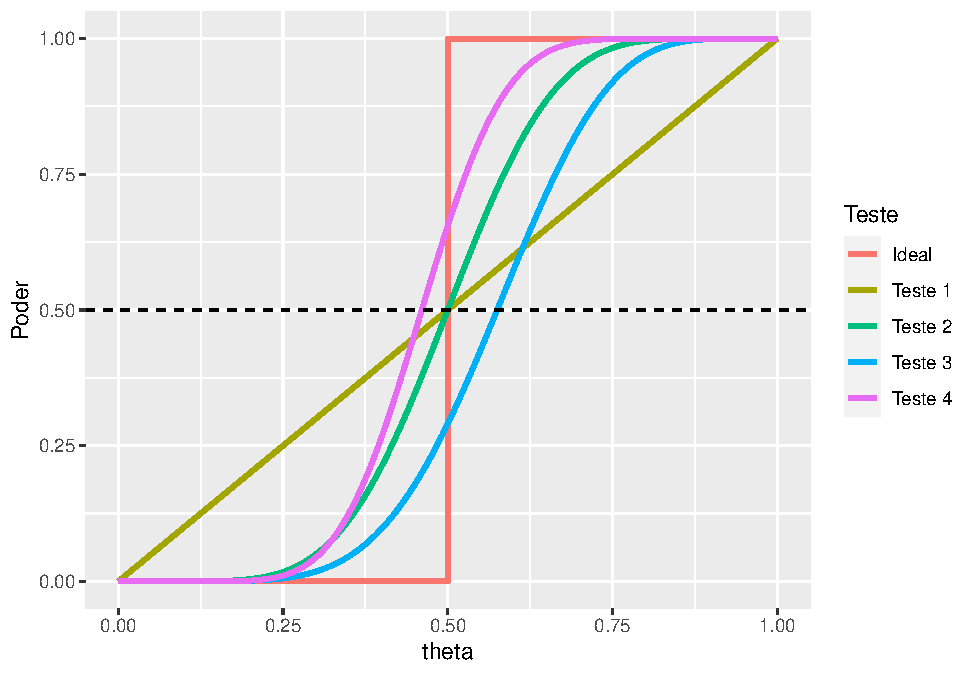
\includegraphics[width=0.8\linewidth]{InfBayes_files/figure-latex/unnamed-chunk-26-1} \end{center}

\(~\)

No exemplo anterior, foi apresentado uma maneira de considerar custos das observações e obter um tamanho amostral ótimo para determinado problema de decisão. Quando o custo está relacionado somente a quantidades monetárias, funções de custo lineares não são as mais adequadas. Para uma discussão bastante didática sobre esse problema, veja o artigo \emph{O Paradoxo de São Petersburgo} (Peixoto, C. M. e Wechsler, S.) no \href{https://www.ime.usp.br/~isbra/boletim/boletim_2013_v06_n02.pdf}{Boletim da ISBrA, 6(2)}.

\(~\)

\hypertarget{Test}{%
\chapter{Testes de Hipóteses}\label{Test}}

\hypertarget{BasTest}{%
\section{Conceitos Básicos}\label{BasTest}}

Uma \textbf{hipótese estatística} é uma afirmação sobre o parâmetro \(\theta\) (ou a família \(\mathcal{P}\)). No caso usual, tem-se duas hipóteses: \(H_0: ~\theta\in\Theta_0~\), chamada de \textbf{hipótese nula}, e \(H_1: ~\theta\in\Theta_1={\Theta}_0^c~\), chamada \textbf{hipótese alternativa}.

\(~\)

Um \textbf{teste de hipótese} é uma regra de decisão \(\varphi: \mathfrak{X} \longrightarrow \{0,1\}\), onde \(\varphi(\boldsymbol{x})=1\) significa rejeitar \(H_0\) (aceitar \(H_1\)) e \(\varphi(\boldsymbol x)=0\), não rejeitar (aceitar) \(H_0\).

\(~\)

Se rejeita-se \(H_0\) (aceita-se \(H_1\)) quando \(H_0\) é verdadeira, comete-se um \textbf{erro do tipo I}. Por outro lado, se não rejeita-se \(H_0\) (aceita \(H_0\)) quando \(H_0\) é falso, ocorre um \textbf{erro do tipo II}.

\(~\)

O conjunto \(\varphi^{-1}(1)=\{\boldsymbol{x} \in \mathfrak{X} :~ \varphi(\boldsymbol{x})=1\}\) recebe o nome de \textbf{região de rejeição} (ou \textbf{região crítica}). A \textbf{função de poder} do teste \(\varphi\) é
\({\pi}_\varphi(\theta)\) \(=P\left(\varphi^{-1}(1)|\theta\right)\)
\(=P\big(\text{'Rejeitar $H_0$'} | \theta\big)\).

\(~\)

Dizemos que um teste \(\varphi\) tem \textbf{nível de significância} \(\alpha\) se \(\displaystyle\sup_{\theta\in\Theta_0}\pi_\varphi(\theta)\leq \alpha\). Se \(\alpha=\displaystyle\sup_{\theta\in\Theta_0}\pi_\varphi(\theta)\) dizemos que o teste é de \textbf{tamanho} \(\alpha\).

\(~\)

Uma hipótese é dita \textbf{simples} se contém apenas um ponto, \(H:\theta=\theta_0\). Caso contrário é chamada de \textbf{hipótese composta}. No caso em que \(H:\theta\in\Theta_0\) é tal que \(\dim(\Theta_0)<\dim(\Theta)\), diz-se que \(H\) é uma \textbf{hipótese precisa} (``\emph{sharp}'').

\(~\)

\hypertarget{revisuxe3o-abordagem-frequentista}{%
\section{Revisão: Abordagem Frequentista}\label{revisuxe3o-abordagem-frequentista}}

Um teste de hipótese ``ideal'' seria aquele que as probabilidades de erros tipo I e tipo II são iguais a zero, isto é, \(\pi_\varphi(\theta)=0\), \(\forall \theta \in \Theta_0\), e \(\pi_\varphi(\theta)=1\), \(\forall \theta \in \Theta_1\). Contudo, não é possível obter tais testes em geral.

A solução usual é fixar um nível de significância \(\alpha\) e considerar apenas a classe de teste de nível \(\alpha\), isto é, testes tais que \(\displaystyle\sup_{\theta\in\Theta_0}\pi_\varphi(\theta) \leq \alpha\). Os testes ótimos sob o ponto de vista frequentista são aqueles na classe de testes de nível alpha que tenha maior função poder \({\pi}_\varphi(\theta)\) para \(\theta \in \Theta_1\). Um teste que satisfaz isso é chamado de \textbf{Teste Uniformemente Mais Poderoso} (\textbf{UMP}) mas testes com essa propriedade também só podem ser obtidos em casos específicos.

\(~\)

\textbf{Exemplo.} Considere que \(\Theta=[0,1]\) e deseja-se testar \(H_0: \theta \leq 0.5\) contra \(H_1: \theta > 0.5\). O gráfico a seguir ilustra as funções poder dos quatro testes disponíveis para esse problema. Supondo (apenas para fins didáticos) que \(\alpha=0.5\), temos que o teste UMP de nível \(\alpha\) é o teste 2. O teste 4, apesar de ser mais poderoso, não é um teste de nível \(\alpha\).

\begin{center}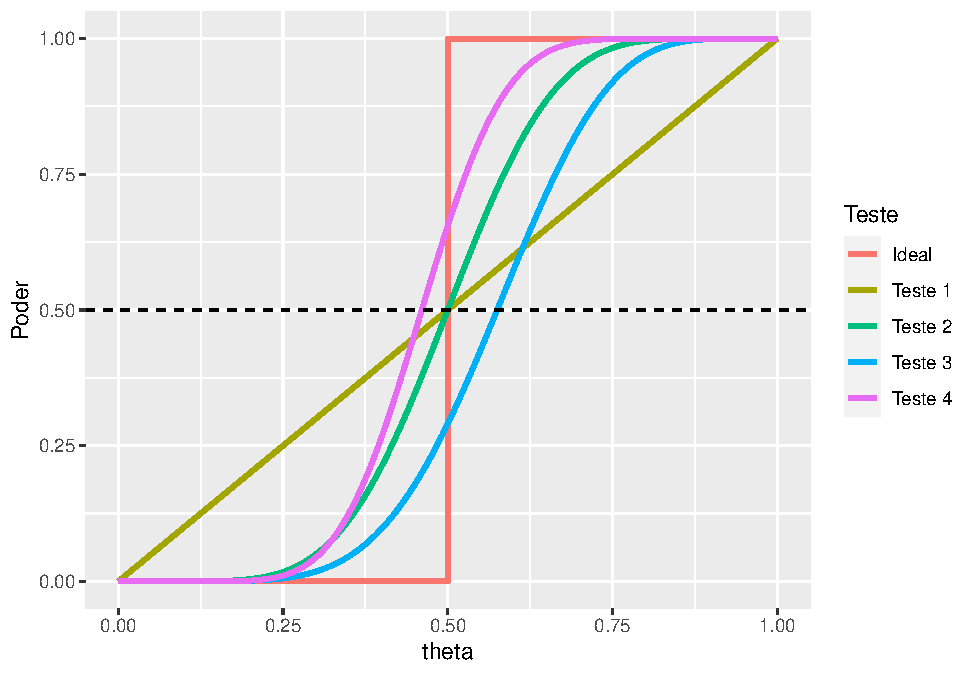
\includegraphics[width=0.8\linewidth]{InfBayes_files/figure-latex/unnamed-chunk-27-1} \end{center}

\(~\)

Uma das situações onde é possível obter o teste mais poderoso é o caso que as hipóteses nula e alternativa são simples, isto é, \(H_0:\theta=\theta_0\) contra \(H_1:\theta=\theta_1\). Nesses casos, pode-se considerar o \textbf{Lema de Neyman-Pearson}, que afirma que o \textbf{teste mais poderoso} é dado por

\({\varphi}^*(\boldsymbol x)=\left\{\begin{array}{rl} 1,& \dfrac{f(x|\theta_0)}{f(x|\theta_1)}\leq k\\ 0,& c.c.\end{array}\right.~.\)

Além disso, o teste \({\varphi}^*\) minimiza a combinação linear das probabilidades de erro \(a\alpha+b\beta\) com \(k=b/a\), \(\alpha={\pi}_{{\varphi}^*}(\theta_0)\) \(=P(\textrm{'erro tipo I'})\) e \(\beta=1-{\pi}_{{\varphi}^*}(\theta_1)\) \(=P(\textrm{'erro tipo II'})\).

\(~\)

Como dito anteriorimente, usualmente é fixado um nível \(\alpha\) e isso permite encontrar o valor de \(k\) de modo que o teste construído a partir do lema é o teste mais poderoso de nível \(\alpha\). Assim,

\(\alpha\) \(={\pi}_{\varphi^*}(\theta_0)\) \(=P\left(\boldsymbol X \in {\varphi}^{-1}(\{1\})|\theta_0\right)\) \(=P\left(\left\{\boldsymbol x: \dfrac{f(\boldsymbol x|\theta_0)}{f(\boldsymbol x|\theta_1)} \leq k\right\}\Big|\theta_0\right)\).

Suponha que foi observado \(\boldsymbol X = \boldsymbol x_o\), é possível calcular o \emph{nível descritivo} (ou \emph{p-value}) da seguinte forma:

\(p(\boldsymbol x_o)\) \(=P\left(\left\{\boldsymbol x: \dfrac{f(\boldsymbol x|\theta_0)}{f(\boldsymbol x|\theta_1)} \leq \dfrac{f(\boldsymbol x_o|\theta_0)}{f(\boldsymbol x_o|\theta_1)}\right\}\Big|\theta_0\right)\)

\(~\)

É possível obter testes UMP em alguns casos particulares. Em especial, nos casos em que a família de distribuições para \(\boldsymbol X\) condicional a \(\theta\) possui a propriedade de \emph{razão de verossimilhanças monótona}, é possível construir testes UMP para hipóteses do tipo \(H_1: \theta \leq \theta_0\) contra \(H_1: \theta > \theta_0\). Para problemas onde as hipóteses são da forma \(H_1: \theta = \theta_0\) contra \(H_1: \theta \neq \theta_0\), bastante comuns no dia a dia de um estatístico, não existe teste UMP, em geral.

\(~\)

Nos casos em que não existe um teste UMP, o teste mais utilizado sob a abordagem frequentista certamente é o \textbf{teste da razão de verossimilhança generalizada} (RVG). Primeiramente, considere a \emph{razão de verossimilhanças generalizada}, dada por

\(\lambda(\boldsymbol x)=\dfrac{\displaystyle \sup_{\theta\in\Theta_0} f(\boldsymbol x|\theta)}{\displaystyle \sup_{\theta\in\Theta} f(\boldsymbol x|\theta)}\).

Note que \(0\leq \lambda(\boldsymbol x) \leq 1\), \(\forall ~\boldsymbol x \in \mathfrak{X}\) e \(\forall ~\Theta_0 \subseteq \Theta\). Um \emph{teste RVG} é qualquer teste da forma

\({\varphi}_{RV}(\boldsymbol x)=\left\{\begin{array}{rl} 1,& \lambda(\boldsymbol x) \leq k\\ 0,& c.c.\end{array}\right.~.\)

\(~\)

Novamente, \(k\) pode ser escolhido de modo que o teste resultante seja de nível \(\alpha\), isto é, \(\displaystyle \sup_{\theta \in \Theta_0} P\left(\lambda(\boldsymbol x) \leq k \Big | \theta\right) \leq \alpha\). Do mesmo modo, se foi observado \(\boldsymbol X=\boldsymbol x_o\), um \emph{p-value} é \(p(\boldsymbol x_o)\) \(=\displaystyle \sup_{\theta \in \Theta_0}P\left(\left\{\boldsymbol x: \lambda(\boldsymbol x) \leq \lambda(\boldsymbol x_o)\right\}\big|\theta\right)\). Por fim, em casos onde é difícil fazer os cálculos de forma exata e o tamanho amostral \(n\) é razoavelmente grande, é possível usar a distribuição assintótica da RVG \(~-2\log \lambda(\boldsymbol x)\overset{\mathcal{D}}{~\longrightarrow~}\chi_d^2\), onde \(d=\dim(\Theta)-\dim(\Theta_0)\).

\(~\)

\(~\)

\hypertarget{abordagem-bayesiana-via-teoria-da-decisuxe3o}{%
\section{Abordagem Bayesiana (via Teoria da Decisão)}\label{abordagem-bayesiana-via-teoria-da-decisuxe3o}}

Sob a abordagem de teoria da decisão, podemos ver um teste de hipóteses como um problema de decisão onde temos duas possíveis decisões \(\mathcal{D}=\{d_0,d_1\}\), onde \(d_0\) é decidir por \(H_0:\theta \in \Theta_0\) e \(d_1\) é decidir por \(H_1:\theta \in \Theta_1\), com \(\Theta=\Theta_0\cup\Theta_1\). Um teste de hipóteses nesse contexto é uma função de decisão \(\varphi: \mathfrak{X} \longrightarrow \{0,1\}\), de modo que quando \(\varphi(\boldsymbol x)=i\), decide-se por \(d_i\), \(i\in \{0,1\}\).

\(~\)

Primeiramente, considere o contexto apresentado no Lema de Neyman-Pearson, onde \(\Theta=\{\theta_0,\theta_1\}\) e deseja-se testar \(H_0: \theta=\theta_0\) contra \(H_1: \theta = \theta_1\). Considere que, a priori, \(f(\theta_0) = \pi\), a função de verossimilhança é \(f(\boldsymbol x |\theta)\) e a função de perda apresentada na tabela a seguir.

\(L(d,\theta)\)

\(\theta_0\)

\(\theta_1\)

\(d_0\)

\(0\)

\(b\)

\(d_1\)

\(a\)

\(0\)

Então, o risco de uma função de decisão \(\varphi\) é

\(\rho(\varphi,P)\) \(=E\left[L(\varphi(\boldsymbol X),\theta)\right]\)
\(= \pi~E\left[L(\varphi(\boldsymbol X),\theta)\big|\theta_0)\right] + (1-\pi)E\left[L(\varphi(\boldsymbol X),\theta)\big|\theta_1)\right]\)
\(= a~\pi~P\left(\varphi(\boldsymbol x)=1\big|\theta_0\right) + b~(1-\pi)~P\left(\varphi(\boldsymbol x)=0\big|\theta_1\right)\)
\(= a~\pi~\alpha_\varphi + b~(1-\pi)~\beta_\varphi\)

Como o risco acima é uma combinação linear das probabilidades dos erro tipo I e tipo II, podemos aplicar o Lema de Neyman-Pearson e obter a função de decisão \(\varphi^*\) que minimiza o risco

\({\varphi}^*(\boldsymbol x)=\left\{\begin{array}{rl} 1,& \dfrac{f(x|\theta_0)}{f(x|\theta_1)}\leq \dfrac{b~(1-\pi)}{a~\pi}\\ 0,& c.c.\end{array}\right.~.\)

Esse resultado é apresentado por DeGroot (1986) e é uma espécie de \emph{Lema de Neyman-Pearson Generalizado}.

\(~\)

A solução para esse mesmo problema pode também ser obtida usando a \emph{forma extensiva}. O risco posterior para as suas decisões é \(r_x(d_0) = b f(\theta_1|\boldsymbol x)\) e \(r_x(d_1) = a f(\theta_0|\boldsymbol x)\), de modo que rejeitamos \(H_0\) (decidimos por \(d_1\) ou \(\varphi(\boldsymbol x)=1\)) se

\(r_x(d_1) \leq r_x(d_0)\)
\(\Longleftrightarrow a f(\theta_0|\boldsymbol x) \leq b f(\theta_1|\boldsymbol x)\)
\(\Longleftrightarrow a f(\theta_0|\boldsymbol x) \leq b \left[1-f(\theta_0|\boldsymbol x)\right]\)
\(\Longleftrightarrow f(\theta_0|\boldsymbol x) \leq \dfrac{b}{a+b}\)

De modo que o teste de Bayes também pode ser apresentado como

\({\varphi}^*(\boldsymbol x)=\left\{\begin{array}{rl} 1,& f(\theta_0|\boldsymbol x) \leq \dfrac{b}{a+b} \\ 0,& c.c.\end{array}\right.~.\)

A interpreção nesse caso é mais direta, a hipótese é rejeitada se sua probabilidade posterior é ``pequena''. Como vimos, essas soluções são equivalentes. De fato,

\begin{itemize}
\item
  \(f(\theta_0|\boldsymbol x)\) \(=\dfrac{f(\theta_0)f(\boldsymbol x|\theta_0)}{f(\boldsymbol x)}\) \(=\pi~\dfrac{f(\boldsymbol x|\theta_0)}{f(\boldsymbol x)}\);
\item
  \(f(\theta_1|\boldsymbol x)\) \(=\dfrac{f(\theta_1)f(\boldsymbol x|\theta_1)}{f(\boldsymbol x)}\) \(=(1-\pi)~\dfrac{f(\boldsymbol x|\theta_1)}{f(\boldsymbol x)}\).
\end{itemize}

Assim,

\(r_x(d_1) \leq r_x(d_0)\)
\(\Longleftrightarrow a \pi~\dfrac{f(\boldsymbol x|\theta_0)}{f(\boldsymbol x)} \leq b (1-\pi)~\dfrac{f(\boldsymbol x|\theta_1)}{f(\boldsymbol x)}\)
\(\Longleftrightarrow \dfrac{f(\boldsymbol x|\theta_0)}{f(\boldsymbol x|\theta_1)} \leq \dfrac{b (1-\pi)}{a \pi}\).

\(~\)

\(~\)

Considere agora um caso mais geral, onde \(\Theta=\Theta_0 \dot{\cup} \Theta_1\) e deseja-se testar \(H_0: \theta \in \Theta_0\) contra \(H_1: \theta \in \Theta_1\). Considere também a função de perda mais geral apresentada a seguir, com \(a_0 \leq a_1\) e \(b_0 \leq b_1\).

\(L(d,\theta)\)

\(\Theta_0\)

\(\Theta_1\)

\(d_0\)

\(a_0\)

\(b_1\)

\(d_1\)

\(a_1\)

\(b_0\)

O risco posterior de cada uma das decisões é

\(r_x(d_0,\theta)\) \(=a_0P(\theta\in\Theta_0|x)+b_1P(\Theta_1|x)\) \(=a_0P(\theta\in\Theta_0|x)+b_1\left[1- P(\Theta_0|x)\right]\) \(=a_0P(\theta\in\Theta_0|x)+b_1-b_1P(\Theta_0|x)\),

\(r_x(d_1,\theta)\) \(=a_1P(\theta\in\Theta_0|x)+b_0-b_0P(\Theta_0|x)\),

De modo que rejeita-se \(H_0\), \(\varphi(\boldsymbol x)=1\), se

\(r_x(d_1,P)\leq r_x(d_0,P)\) \(\Leftrightarrow (a_1-b_0)P(\Theta_0|x)+b_0 \leq (a_0-b_1)P(\Theta_0|x)+b_1\) \(\Leftrightarrow P(\Theta_0|x) \leq \dfrac{(b_1-b_0)}{(a_1-a_0)+(b_1-b_0)}\)

Assim, o teste de bayes nesse caso é

\({\varphi}(\boldsymbol x)=\left\{\begin{array}{rl} 1,& P(\Theta_0|x) \leq \dfrac{(b_1-b_0)}{(a_1-a_0)+(b_1-b_0)} \\ 0,& c.c.\end{array}\right.~.\)

\(~\)

\(~\)

\hypertarget{probabilidade-posterior-de-h_0}{%
\section{\texorpdfstring{Probabilidade Posterior de \(H_0\)}{Probabilidade Posterior de H\_0}}\label{probabilidade-posterior-de-h_0}}

\textbf{Resultado.} Seja \(\Theta=\Theta_0 \dot{\cup} \Theta_1\) e suponha que deseja-se testar \(H_0: \theta \in \Theta_0\) contra \(H_1: \theta \in \Theta_1\) considerando a função de perda a seguir, com \(a_0 \leq a_1\) e \(b_0 \leq b_1\).

\(L(d,\theta)\)

\(\Theta_0\)

\(\Theta_1\)

\(d_0\)

\(a_0\)

\(b_1\)

\(d_1\)

\(a_1\)

\(b_0\)

Então, o teste de bayes é

\({\varphi}(\boldsymbol x)=\left\{\begin{array}{rl} 1,& P(\Theta_0|x) \leq \dfrac{(b_1-b_0)}{(a_1-a_0)+(b_1-b_0)} \\ 0,& c.c.\end{array}\right.\).

\(~\)

\textbf{Exemplo 1.} Considere \(X_1,\ldots,X_n\) c.i.i.d. tais que \(X_i|\theta \sim Ber(\theta)\) com \(\Theta = \left\{1/2,3/4\right\}\). Suponha que, a priori, \(f(\theta=1/2)=f(\theta=3/4)=1/2\) e deseja-se testar \(H_0: \theta=1/2\) contra \(H_1: \theta=3/4\). Tem-se que \(T(\boldsymbol X)=\sum X_i~|~\theta\sim Bin(n,\theta)\) é uma estatística suficiente para \(\theta\). Então,

\(P(\theta=1/2|T(\boldsymbol X)=t)\) \(=\dfrac{f(t|\theta=1/2)f(\theta=1/2)}{\displaystyle\sum_{\theta \in \left\{1/2~,~3/4\right\}} f(t|\theta)f(\theta)}\) \(=\dfrac{\displaystyle\binom{n}{t}\left(\dfrac{1}{2}\right)^n}{\displaystyle\binom{n}{t}\left(\dfrac{1}{2}\right)^n+\binom{n}{t}\left(\dfrac{3}{4}\right)^t\left(\dfrac{1}{4}\right)^{n-t}}\) \(=\dfrac{1}{1+\dfrac{3^t}{2^n}}\).

\(~\)

Considere a função de perda \(L(d,\theta) = a_0~\mathbb{I}(d_0,\Theta_0) + b_1~\mathbb{I}(d_0,\Theta_1) + a_1~\mathbb{I}(d_1,\Theta_0) + b_0~\mathbb{I}(d_1,\Theta_1)\) como no resultado anterior. Então, rejeita-se \(H_0\) se \(P(\theta \in \Theta_0 | \boldsymbol x) < K\), com \(K = \dfrac{b_1-b_0}{(a_1-a_0)+(b_1-b_0)}\). Assim,

\(P(\theta=1/2|T=t)\leq K\)
\(~\Longleftrightarrow~ \dfrac{1}{1+\frac{3^t}{2^n}} \leq K\)
\(~\Longleftrightarrow~ {1+\dfrac{3^t}{2^n}} \geq \dfrac{1}{K}\)
\(~\Longleftrightarrow~ 3^t\geq 2^n\left(\dfrac{1}{K}-1\right)\)
\(~\Longleftrightarrow~ t\geq n\log_3(2)+\log_3\left(\dfrac{1-K}{K}\right)\) \(~\Longleftrightarrow~ t\geq nlog_3(2)+log_3\left(\dfrac{a_1-a_0}{b_1-b_0}\right)\).

\(~\)

Tomando \(a_1=b_1=1\) e \(a_0=b_0=0\), rejeita \(H\) se

\(\sum X_i \geq n\log_3(2)+\log_3(1)\) \(~\Longleftrightarrow~ \sum X_i \geq n\log_3(2)\)
\(~\Longrightarrow~ \bar{X} \geq \log_3(2)\approx 0,631\).

\(~\)

O teste de Bayes é

\({\varphi}(\boldsymbol x) =\left\{\begin{array}{rl} 1,& f(\theta=1/2|\boldsymbol x) \leq \dfrac{(b_1-b_0)}{(a_1-a_0)+(b_1-b_0)} = \dfrac{1}{2} \\ 0,& c.c.\end{array}\right.\)
\(~\Longrightarrow~ {\varphi}(\boldsymbol x) =\left\{\begin{array}{rl} 1,& \bar{X} \geq \log_3(2) \\ 0,& c.c.\end{array}\right.\).

\(~\)

\(~\)

\textbf{Exemplo 2:} \(X_1,...,X_n\) c.i.i.d. tais que \(X_i|\theta\sim N(\theta,{\sigma}_0^2)\) com \({\sigma}_0^2\) conhecido. Suponha que, a priori, \(\theta \sim N(m,v^2)\) e \(\bar{X}\) é estatística suficiente para \(\theta\) com \(\bar{X}|\theta \sim \left(\theta,{\sigma}_0^2/n\right)\), de modo que \(\theta|\boldsymbol X \sim N\left(\dfrac{{\sigma}_0^2~m+nv^2~\bar x}{{\sigma}_0^2+nv^2}~,~\dfrac{{\sigma}_0^2~v^2}{{\sigma}_0^2+nv^2}\right)\). Suponha ainda que o objetivo é testar \(H_0: \theta\leq \theta_0\) contra \(H_1:\theta > \theta_0\).

\(~\)

Utilizando novamente o resultado anterior, temos

\(P\left(\theta\in\Theta_0|\boldsymbol x\right)\)
\(= P\left(\theta \leq \theta_0|\boldsymbol x\right)\)
\(= P\left(Z\leq\dfrac{\theta_0-\frac{{\sigma}_0^2~m+nv^2~\bar x}{{\sigma}_0^2+nv^2}}{\sqrt{\frac{{\sigma}_0^2~v^2}{{\sigma}_0^2+nv^2}}}~\Bigg|~\bar x\right)\)
\(= \Phi\left(\dfrac{\theta_0-\frac{{\sigma}_0^2~m+nv^2~\bar x}{{\sigma}_0^2+nv^2}}{\sqrt{\frac{{\sigma}_0^2~v^2}{{\sigma}_ 0^2+nv^2}}}\right)\)
\(= \Phi\left(\dfrac{({\sigma}_0^2+nv^2)\theta_0-{\sigma}_0^2~m-nv^2~\bar x}{{\sigma}_0~v~\sqrt{{\sigma}_ 0^2+nv^2}}\right)\),

e deve-se rejeitar \(H_0\) se

\(P\left(\theta\in\Theta_0|\boldsymbol x\right) \leq \dfrac{(b_1-b_0)}{(a_1-a_0)+(b_1-b_0)} = K\)
\(~\Longleftrightarrow~\Phi\left(\dfrac{({\sigma}_0^2+nv^2)\theta_0-{\sigma}_0^2~m-nv^2~\bar x}{{\sigma}_0~v~\sqrt{{\sigma}_ 0^2+nv^2}}\right) \leq K\)
\(~\Longleftrightarrow~ \bar x ~\geq~ \dfrac{({\sigma}_0^2+nv^2)\theta_0-{\sigma}_0^2~m}{nv^2} - {\Phi}^{-1}(K)\dfrac{{\sigma}_0~\sqrt{{\sigma}_ 0^2+nv^2}}{nv}\)
\(~\Longleftrightarrow~ \bar x ~\geq~ \dfrac{{\sigma}_0^2(\theta_0-m)+nv^2\theta_0}{nv^2} - {\Phi}^{-1}(K)\dfrac{{\sigma}_0~\sqrt{{\sigma}_ 0^2+nv^2}}{nv}\).

\(~\)

Se \(a_0=b_0=0\) e \(a_1=b_1=1\), então \(\Phi^{-1}(K=1/2)=0\) e rejeita-se \(H_0\) se

\(\bar x ~\geq~ \dfrac{{\sigma}_0^2(\theta_0-m)+nv^2\theta_0}{nv^2} ~\underset{n\uparrow\infty}{\longrightarrow}~ \theta_0\).

\(~\)

\(~\)

\hypertarget{fator-de-bayes}{%
\section{Fator de Bayes}\label{fator-de-bayes}}

Voltando ao resultado, tem-se que rejeita-se \(H_0\) se

\(r_x(d_0) \geq r_x(d_1)\)
\(~\Longleftrightarrow~ a_0P(\Theta_0|\boldsymbol x)+b_1P(\Theta_1|\boldsymbol x) \geq a_1P(\Theta_0|\boldsymbol x)+b_0P(\Theta_1|\boldsymbol x)\)
\(~\Longleftrightarrow~ \dfrac{P(\Theta_0|\boldsymbol x)}{P(\Theta_1|\boldsymbol x)}\leq\dfrac{b_1-b_0}{a_1-a_0}\)

\(~\Longleftrightarrow~ BF(\boldsymbol x)\) \(=\dfrac{\frac{P(\Theta_0|\boldsymbol x)}{P(\Theta_1|\boldsymbol x)}}{\frac{P(\Theta_0)}{P(\Theta_1)}}\) \(=\dfrac{\frac{P(\Theta_0|\boldsymbol x)}{P(\Theta_0)}}{\frac{P(\Theta_1|\boldsymbol x)}{P(\Theta_1)}}\)
\(=\dfrac{f(\boldsymbol x | \Theta_0)}{f(\boldsymbol x | \Theta_1)}\)
\(\leq \dfrac{(b_1-b_0)}{(a_1-a_0)}\dfrac{P(\Theta_1)}{P(\Theta_0)}\),

onde \(BF\) é o \textbf{Fator de Bayes}, frequentemente utilizado na literatura bayesiana para testar hipóteses. Ele pode ser visto como uma razão de chances que representa o aumento na chance da hipótese nula ser mais plausível que a hipótese alternativa após observar os dados em relação a sua opinião a priori. O \(BF\) também pode ser reescrito como

\(BF(\boldsymbol x)\)
\(=\dfrac{f_0(\boldsymbol x)}{f_1(\boldsymbol x)}\)
\(=\dfrac{f(\boldsymbol x | \Theta_0)}{f(\boldsymbol x | \Theta_1)}\)
\(=\dfrac{\displaystyle \int_{\Theta}f(\boldsymbol x|\theta) f(\theta|\Theta_0) d\theta} {\displaystyle \int_{\Theta} f(\boldsymbol x|\theta)f(\theta|\Theta_1)d\theta}\)
\(=\dfrac{\displaystyle \int_{\Theta_0}f(x|\theta)dP_0(\theta)}{\displaystyle \int_{\Theta_1}f(x|\theta)dP_1(\theta)}\)
\(=\dfrac{E\left[f(\boldsymbol x|\theta)|\theta\in\Theta_0\right]}{E\left[f(\boldsymbol x|\theta)|\theta \in \Theta_1\right]}\).

\(~\)

\textbf{No exemplo 1.} Lembrando que, a priori, \(P(\theta=1/2)=P(\theta=3/4)=1/2\) e considerando novamente \(a_0=b_0=0\) e \(a_1=b_1=1\), temos que devemos rejeitar \(H_0\) se \(BF(\boldsymbol x)<\frac{(b_1-b_0)}{(a_1-a_0)}\frac{P(\theta=1/2)}{P(\theta=3/4)}=1\). Então,

\(BF(\boldsymbol x)=\dfrac{P(\theta=1/2|\boldsymbol x)}{P(\theta=3/4|\boldsymbol x)}\dfrac{1/2}{1/2}\) \(=\dfrac{\frac{1}{1+3^t/2^n}}{\frac{3^t/2^n}{1+3^t/2^n}}\) \(=\dfrac{2^n}{3^t}\leq 1\) \(~\Longleftrightarrow~ \bar{x} \geq \log_3(2)\),

de modo que a decisão baseada no fator de Bayes concorda com o resultado baseado na probabilidade a posteriori da hipótese.

\(~\)

\textbf{No exemplo 2.} \(\theta|\boldsymbol X \sim N\left(\dfrac{{\sigma}_0^2~m+nv^2~\bar x}{{\sigma}_0^2+nv^2}~,~\dfrac{{\sigma}_0^2~v^2}{{\sigma}_0^2+nv^2}\right)\) e o objetivo é testar \(H_0: \theta\leq \theta_0\) contra \(H_1:\theta > \theta_0\). A probabilidade a posteriori da hipótese \(H_0\) é

\(P\left(\theta\in\Theta_0|\boldsymbol x\right)\)
\(= \Phi\left(\dfrac{({\sigma}_0^2+nv^2)\theta_0-{\sigma}_0^2~m-nv^2~\bar x}{{\sigma}_0~v~\sqrt{{\sigma}_ 0^2+nv^2}}\right)\),

e, a priori, \(P(\theta \in \Theta_0)\) \(=P(\theta \leq \theta_0)\) \(= \Phi\left(\dfrac{\theta_0-m}{v}\right)\), de modo que o fator de Bayes nesse caso é

\(BF(\boldsymbol x)\)
\(= \dfrac{P(\Theta_0|\boldsymbol x)}{P(\Theta_1|\boldsymbol x)} \dfrac{P(\Theta_1)}{P(\Theta_0)}\)
\(= \dfrac{\Phi\left(\frac{({\sigma}_0^2+nv^2)\theta_0-{\sigma}_0^2~m-nv^2~\bar x}{{\sigma}_0~v~\sqrt{{\sigma}_0^2+nv^2}}\right)}{\left[1-\Phi\left(\frac{({\sigma}_0^2+nv^2)\theta_0-{\sigma}_0^2~m-nv^2~\bar x}{{\sigma}_0~v~\sqrt{{\sigma}_0^2+nv^2}}\right)\right]} ~ \dfrac{\left[1-\Phi\left(\frac{\theta_0-m}{v}\right)\right]}{\Phi\left(\frac{\theta_0-m}{v}\right)}\).

\(~\)

\begin{Shaded}
\begin{Highlighting}[]
\NormalTok{m=}\DecValTok{0}\NormalTok{; v2=}\DecValTok{1} \CommentTok{# Média e Variância da Priori}
\NormalTok{sigma02=}\DecValTok{1} \CommentTok{# Variância Populacional (conhecido)}
\NormalTok{n=}\DecValTok{3} \CommentTok{# tamanho amostral}
\NormalTok{theta0=}\DecValTok{1} \CommentTok{# H0: theta <= theta0}
\NormalTok{a0=}\DecValTok{0}\NormalTok{; b0=}\DecValTok{0}\NormalTok{; a1=}\DecValTok{1}\NormalTok{; b1=}\DecValTok{1} \CommentTok{# Função de Perda}
\NormalTok{K1=(b1}\OperatorTok{-}\NormalTok{b0)}\OperatorTok{/}\NormalTok{(a1}\OperatorTok{-}\NormalTok{a0}\OperatorTok{+}\NormalTok{b1}\OperatorTok{-}\NormalTok{b0) }\CommentTok{# corte Prob. Posterior}
\NormalTok{K2=((b1}\OperatorTok{-}\NormalTok{b0)}\OperatorTok{*}\NormalTok{(}\DecValTok{1}\OperatorTok{-}\KeywordTok{pnorm}\NormalTok{((theta0}\OperatorTok{-}\NormalTok{m)}\OperatorTok{/}\KeywordTok{sqrt}\NormalTok{(v2)))) }\OperatorTok{/}\StringTok{ }\NormalTok{((a1}\OperatorTok{-}\NormalTok{a0)}\OperatorTok{*}\KeywordTok{pnorm}\NormalTok{((theta0}\OperatorTok{-}\NormalTok{m)}\OperatorTok{/}\KeywordTok{sqrt}\NormalTok{(v2))) }\CommentTok{#corte Fator de Bayes}
\NormalTok{K3=((sigma02}\OperatorTok{+}\NormalTok{n}\OperatorTok{*}\NormalTok{v2)}\OperatorTok{*}\NormalTok{theta0}\OperatorTok{-}\NormalTok{sigma02}\OperatorTok{*}\NormalTok{m)}\OperatorTok{/}\NormalTok{(n}\OperatorTok{*}\NormalTok{v2) }\OperatorTok{-}\StringTok{ }\KeywordTok{qnorm}\NormalTok{(K1)}\OperatorTok{*}\KeywordTok{sqrt}\NormalTok{(sigma02}\OperatorTok{*}\NormalTok{(sigma02}\OperatorTok{+}\NormalTok{n}\OperatorTok{*}\NormalTok{v2))}\OperatorTok{/}\NormalTok{(n}\OperatorTok{*}\KeywordTok{sqrt}\NormalTok{(v2)) }\CommentTok{# corte xbar}
\CommentTok{# Probabilidade a Posteriori de H0 (como função de Xbar)}
\NormalTok{postH =}\StringTok{ }\ControlFlowTok{function}\NormalTok{(xbar)\{}
  \KeywordTok{pnorm}\NormalTok{(((sigma02 }\OperatorTok{+}\StringTok{ }\NormalTok{n}\OperatorTok{*}\NormalTok{v2)}\OperatorTok{*}\NormalTok{theta0 }\OperatorTok{-}\StringTok{ }\NormalTok{sigma02}\OperatorTok{*}\NormalTok{m }\OperatorTok{-}\StringTok{ }\NormalTok{n}\OperatorTok{*}\NormalTok{v2}\OperatorTok{*}\NormalTok{xbar)}\OperatorTok{/}\StringTok{ }\KeywordTok{sqrt}\NormalTok{(sigma02}\OperatorTok{*}\NormalTok{v2}\OperatorTok{*}\NormalTok{(sigma02}\OperatorTok{+}\NormalTok{n}\OperatorTok{*}\NormalTok{v2))) \}}
\CommentTok{# Fator de Bayes de H0 (como função de Xbar)}
\NormalTok{bf =}\StringTok{ }\ControlFlowTok{function}\NormalTok{(xbar)\{}
\NormalTok{  (}\KeywordTok{postH}\NormalTok{(xbar)}\OperatorTok{*}\NormalTok{(}\DecValTok{1}\OperatorTok{-}\KeywordTok{pnorm}\NormalTok{((theta0}\OperatorTok{-}\NormalTok{m)}\OperatorTok{/}\KeywordTok{sqrt}\NormalTok{(v2))))}\OperatorTok{/}\StringTok{ }\NormalTok{((}\DecValTok{1}\OperatorTok{-}\KeywordTok{postH}\NormalTok{(xbar))}\OperatorTok{*}\KeywordTok{pnorm}\NormalTok{((theta0}\OperatorTok{-}\NormalTok{m)}\OperatorTok{/}\KeywordTok{sqrt}\NormalTok{(v2))) \}}
\NormalTok{xbar=}\KeywordTok{seq}\NormalTok{(}\FloatTok{0.5}\NormalTok{,}\FloatTok{2.5}\NormalTok{,}\FloatTok{0.001}\NormalTok{)}
\NormalTok{PP=}\KeywordTok{postH}\NormalTok{(xbar)}
\NormalTok{BF=}\KeywordTok{bf}\NormalTok{(xbar)}
\NormalTok{FS=(}\KeywordTok{max}\NormalTok{(PP)}\OperatorTok{-}\KeywordTok{min}\NormalTok{(PP))}\OperatorTok{/}\NormalTok{(}\KeywordTok{max}\NormalTok{(BF)}\OperatorTok{-}\KeywordTok{min}\NormalTok{(BF)) }\CommentTok{# var. aux. para transformção dos eixos}
\KeywordTok{tibble}\NormalTok{(xbar,PP,BF) }\OperatorTok
\StringTok{  }\KeywordTok{ggplot}\NormalTok{() }\OperatorTok{+}
\StringTok{    }\KeywordTok{geom_line}\NormalTok{(}\KeywordTok{aes}\NormalTok{(}\DataTypeTok{x=}\NormalTok{xbar,}\DataTypeTok{y=}\NormalTok{PP,}\DataTypeTok{colour=}\StringTok{"Prob. Posterior"}\NormalTok{)) }\OperatorTok{+}
\StringTok{    }\KeywordTok{geom_line}\NormalTok{(}\KeywordTok{aes}\NormalTok{(}\DataTypeTok{x=}\NormalTok{xbar,}\DataTypeTok{y=}\NormalTok{((BF}\OperatorTok{-}\KeywordTok{min}\NormalTok{(BF))}\OperatorTok{*}\NormalTok{FS}\OperatorTok{+}\KeywordTok{min}\NormalTok{(PP)),}\DataTypeTok{colour=}\StringTok{"Fator de Bayes"}\NormalTok{))}\OperatorTok{+}
\StringTok{    }\KeywordTok{scale_y_continuous}\NormalTok{(}\DataTypeTok{sec.axis =} \KeywordTok{sec_axis}\NormalTok{(}\OperatorTok{~}\NormalTok{.}\OperatorTok{/}\NormalTok{FS}\OperatorTok{-}\KeywordTok{min}\NormalTok{(PP)}\OperatorTok{/}\NormalTok{FS}\OperatorTok{+}\KeywordTok{min}\NormalTok{(BF), }\DataTypeTok{name =} \StringTok{"BF"}\NormalTok{))}\OperatorTok{+}
\StringTok{    }\KeywordTok{geom_hline}\NormalTok{(}\KeywordTok{aes}\NormalTok{(}\DataTypeTok{yintercept=}\NormalTok{K1),}\DataTypeTok{lty=}\DecValTok{2}\NormalTok{, }\DataTypeTok{col=}\StringTok{"darkgrey"}\NormalTok{) }\OperatorTok{+}
\StringTok{    }\KeywordTok{geom_point}\NormalTok{(}\KeywordTok{aes}\NormalTok{(}\DataTypeTok{x=}\NormalTok{K3,}\DataTypeTok{y=}\NormalTok{K1,}\DataTypeTok{colour=}\StringTok{"Prob. Posterior"}\NormalTok{)) }\OperatorTok{+}
\StringTok{    }\KeywordTok{geom_hline}\NormalTok{(}\KeywordTok{aes}\NormalTok{(}\DataTypeTok{yintercept=}\NormalTok{((K2}\OperatorTok{-}\KeywordTok{min}\NormalTok{(BF))}\OperatorTok{*}\NormalTok{FS}\OperatorTok{+}\KeywordTok{min}\NormalTok{(PP))),}\DataTypeTok{lty=}\DecValTok{2}\NormalTok{, }\DataTypeTok{col=}\StringTok{"darkgrey"}\NormalTok{) }\OperatorTok{+}
\StringTok{    }\KeywordTok{geom_point}\NormalTok{(}\KeywordTok{aes}\NormalTok{(}\DataTypeTok{x=}\NormalTok{K3,}\DataTypeTok{y=}\NormalTok{((K2}\OperatorTok{-}\KeywordTok{min}\NormalTok{(BF))}\OperatorTok{*}\NormalTok{FS}\OperatorTok{+}\KeywordTok{min}\NormalTok{(PP)),}\DataTypeTok{colour=}\StringTok{"Fator de Bayes"}\NormalTok{)) }\OperatorTok{+}
\StringTok{    }\KeywordTok{geom_vline}\NormalTok{(}\KeywordTok{aes}\NormalTok{(}\DataTypeTok{xintercept=}\NormalTok{K3),}\DataTypeTok{lty=}\DecValTok{2}\NormalTok{, }\DataTypeTok{col=}\StringTok{"darkgrey"}\NormalTok{) }\OperatorTok{+}
\StringTok{    }\KeywordTok{theme_bw}\NormalTok{() }\OperatorTok{+}\StringTok{ }\KeywordTok{labs}\NormalTok{(}\DataTypeTok{colour =} \StringTok{""}\NormalTok{)}
\end{Highlighting}
\end{Shaded}

\begin{center}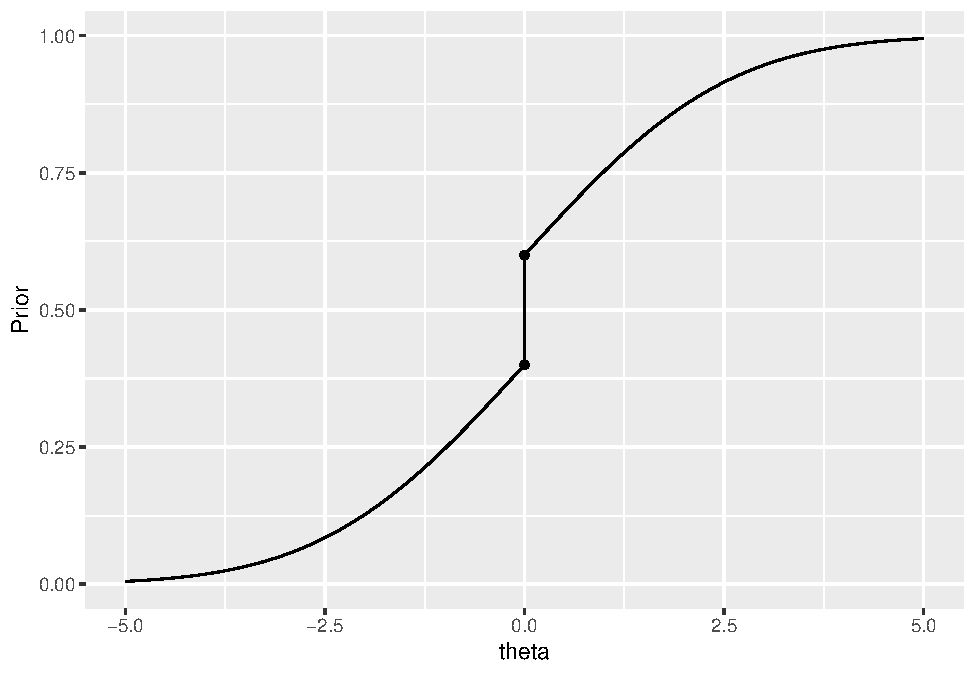
\includegraphics[width=0.8\linewidth]{InfBayes_files/figure-latex/unnamed-chunk-31-1} \end{center}

Nesse exemplo, é possível ver que tanto o Fator de Bayes quanto a probabilidade posterior da hipótese nula ``ordenam'' o espaço amostral, representado aqui pela estatística suficiente, \(\bar{X}\). Deste modo, quanto menores os valores dessas estatísticas de teste, mais desfavorável é o ponto amostral para a hipótese nula. Como visto anteriormente, as regras de decisão baseadas nessas estatísticas são equivalentes e, portanto, a ordenação do espaço amostral é a mesma.

\(~\)

\(~\)

\textbf{Problema:} Suponha agora que, nesse mesmo exemplo, deseja-se testar \(H_0:\theta=0\) contra \(H_1: \theta\neq 0\). Como a posteriori é Normal, temos que \(P(\theta \in \Theta_0|\boldsymbol x)\) \(=P(\theta=0|\boldsymbol x)=0\) , \(\forall~ \boldsymbol x\in \mathfrak{X}~\) e, desta forma, a hipótese nula \(H_0\) sempre é rejeitada.

De fato, para qualquer cenário em que a hipótese \(H_0\) tem medida nula a priori, \(P(\theta \in \Theta_0)=0\), tem-se que, a posteriori, \(P(\theta \in \Theta_0|\boldsymbol x)=0\). Isso ocorre frequentemente nos casos em que \(H_0\) é uma \emph{hipótese precisa}, isto é, \(dim(\Theta_0)<dim(\Theta)\). Neste cenário, é necessário definir procedimentos alternativos para testar hipóteses.

\(~\)

\(~\)

\hypertarget{teste-de-jeffreys}{%
\section{Teste de Jeffreys}\label{teste-de-jeffreys}}

O teste de Jeffreys (1961?) consiste em atribuir uma probabilidade positiva para o conjunto que define a hipótese nula, \(p_0=P(\theta \in \Theta_0)>0\).

\(~\)

\emph{Exemplo 2.} Suponha que deseja-se testar \(H_0: \theta=0\) contra \(H_1: \theta\neq 0\). Suponha que sua opinião a priori é \(\theta \sim Normal(0,2)\). Contudo, já foi visto que \(P(\theta=0|\boldsymbol x)=0\), \(\forall \boldsymbol x \in \mathfrak{X}\). Deste modo, você opta por atribuir uma probabilidade positiva \(p_0=0.2\) para o ponto \(\theta=0\), ou seja, você vai considerar uma distribuição mista \(f(\theta)=p_0\mathbb{I}(\theta=0)+(1-p_0)f_N(\theta)\), onde \(f_N\) é a densidade da \(Normal(0,1)\). Sua função de distribuição a prioi, \(F(\theta)=p_0~\mathbb{I}(\theta\geq0)+(1-p_0)~\Phi\left(\theta/\sqrt{2}\right)\), está representada no gráfico a seguir.

\begin{Shaded}
\begin{Highlighting}[]
\NormalTok{theta=}\KeywordTok{c}\NormalTok{(}\KeywordTok{seq}\NormalTok{(}\OperatorTok{-}\DecValTok{5}\NormalTok{,}\OperatorTok{-}\FloatTok{0.001}\NormalTok{,}\FloatTok{0.001}\NormalTok{),}\KeywordTok{seq}\NormalTok{(}\FloatTok{0.001}\NormalTok{,}\DecValTok{5}\NormalTok{,}\FloatTok{0.001}\NormalTok{))}
\NormalTok{p=}\FloatTok{0.2}
\NormalTok{pprior =}\StringTok{ }\ControlFlowTok{function}\NormalTok{(t)\{}
\NormalTok{  p}\OperatorTok{*}\KeywordTok{I}\NormalTok{(t}\OperatorTok{>=}\DecValTok{0}\NormalTok{)}\OperatorTok{+}\NormalTok{(}\DecValTok{1}\OperatorTok{-}\NormalTok{p)}\OperatorTok{*}\KeywordTok{pnorm}\NormalTok{(t,}\DecValTok{0}\NormalTok{,}\DecValTok{2}\NormalTok{)}\OperatorTok{*}\KeywordTok{I}\NormalTok{(t}\OperatorTok{!=}\DecValTok{0}\NormalTok{)}
\NormalTok{\}}
\KeywordTok{tibble}\NormalTok{(theta,}\DataTypeTok{Prior=}\KeywordTok{pprior}\NormalTok{(theta)) }\OperatorTok
\StringTok{  }\KeywordTok{ggplot}\NormalTok{()}\OperatorTok{+}\KeywordTok{geom_line}\NormalTok{(}\KeywordTok{aes}\NormalTok{(}\DataTypeTok{x=}\NormalTok{theta,}\DataTypeTok{y=}\NormalTok{Prior))}\OperatorTok{+}
\StringTok{    }\KeywordTok{geom_point}\NormalTok{(}\KeywordTok{aes}\NormalTok{(}\DataTypeTok{x=}\DecValTok{0}\NormalTok{,}\DataTypeTok{y=}\NormalTok{(}\DecValTok{1}\OperatorTok{-}\NormalTok{p)}\OperatorTok{*}\KeywordTok{pnorm}\NormalTok{(}\DecValTok{0}\NormalTok{,}\DecValTok{0}\NormalTok{,}\DecValTok{2}\NormalTok{)))}\OperatorTok{+}
\StringTok{    }\KeywordTok{geom_point}\NormalTok{(}\KeywordTok{aes}\NormalTok{(}\DataTypeTok{x=}\DecValTok{0}\NormalTok{,}\DataTypeTok{y=}\NormalTok{(}\DecValTok{1}\OperatorTok{-}\NormalTok{p)}\OperatorTok{*}\KeywordTok{pnorm}\NormalTok{(}\DecValTok{0}\NormalTok{,}\DecValTok{0}\NormalTok{,}\DecValTok{2}\NormalTok{)}\OperatorTok{+}\NormalTok{p))}
\end{Highlighting}
\end{Shaded}

\begin{center}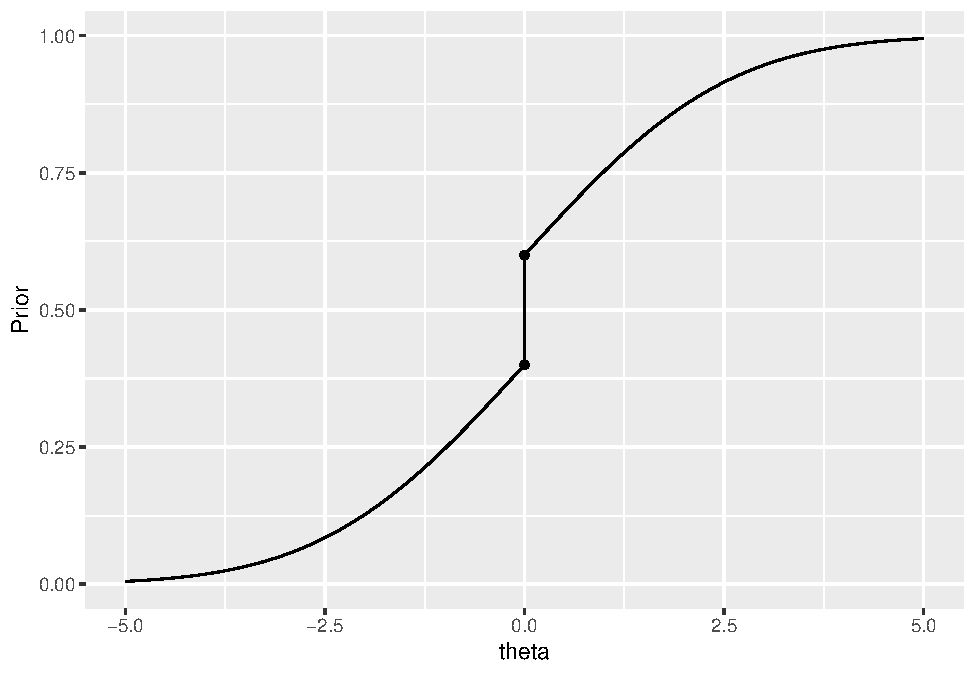
\includegraphics[width=0.8\linewidth]{InfBayes_files/figure-latex/unnamed-chunk-32-1} \end{center}

\textbf{Exercício.} Calcule \(P(\theta=0|\boldsymbol X=\boldsymbol x)\).

\(~\)

\textbf{Exemplo 3.} Seja \(X_1,\ldots,X_n\) c.i.i.d. tais que \(X_i|\theta \sim Ber (\theta)\) e considere que, a priori, \(\theta\sim Beta(a,b)\). Como \(X=\sum X_i\) é estatística suficiente com \(X\big|\theta \sim Bin(n,\theta)\), tem-se que \(\theta\big|x=\sum x_i\sim Beta\left(a+\sum x_i,b+n-\sum x_i\right)\).

A distribuição marginal de \(X\) é chamada \textbf{distribuição preditiva a priori} e pode ser calculada por

\(f(x)\) \(=\displaystyle \int_0^1 f(x,\theta)d\theta\)
\(=\displaystyle \int_0^1 f(x|\theta)f(\theta)d\theta\)
\(=\displaystyle \binom{n}{x}~\dfrac{\Gamma(a+b)}{\Gamma(a)\Gamma(b)}~\int_0^1 \theta^{a+x-1}(1-\theta)^{b+n-x-1}d\theta\)
\(=\displaystyle \binom{n}{x}~\dfrac{\Gamma(a+b)}{\Gamma(a)\Gamma(b)}~\dfrac{\Gamma(a+x)\Gamma(b+n-x)}{\Gamma(a+b+n)}\)
\(=\displaystyle \binom{n}{x} \dfrac{\beta(a+x,b+n-x)}{\beta(a,b)}~\mathbb{I}_{\{0,\ldots,n\}}(x)\)

\(\Longrightarrow X \sim Beta-Binomial(n,a,b)\).

\(~\)

Suponha agora que deseja-se testar \(H_0: \theta=\theta_0\) contra \(H_1:\theta\neq \theta_0\), com \(\theta_0=1/2\), utilizando o teste de Jeffreys. Desta forma, considere \(p_0=P(\theta=1/2)=1/2\) e sua \emph{priori de Jeffreys} é \(f_J(\theta)=p_0~\mathbb{I}(\theta=\theta_0) +(1-p_0)f_\beta(\theta)~\mathbb{I}(\theta\neq\theta_0)\), onde \(f_\beta\) é a densidade da \(Beta(a,b)\).

\begin{center}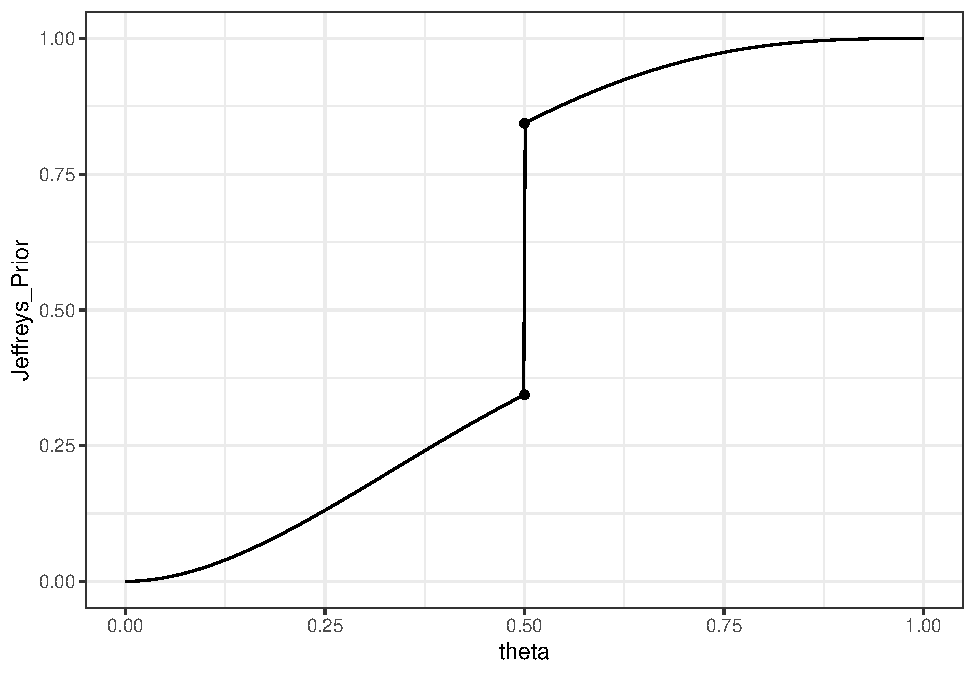
\includegraphics[width=0.8\linewidth]{InfBayes_files/figure-latex/unnamed-chunk-33-1} \end{center}

A distribuição preditiva com relação a priori \(f_J\) é

\(f_J(x)\) \(=\displaystyle p_0f(x|\theta_0)~\mathbb{I}(\theta=\theta_0)+ (1-p_0)\overbrace{\int_0^1f(x|\theta)f_\beta(\theta)~\mathbb{I}(\theta\neq\theta_0)d\theta}^{f(x)}\)
\(=\displaystyle p_0\binom{n}{x}{\theta}_0^x(1-\theta_0)^{n-x}~\mathbb{I}(\theta=\theta_0) + (1-p_0)\binom{n}{x}\dfrac{\beta(a+x,b+n-x)}{\beta(a,b)}~\mathbb{I}(\theta\neq\theta_0)\),

de modo que a distribuição a posteriori é

\(f_J(\theta| x)\) \(= \dfrac{f( x|\theta)f_J(\theta)}{f_J(x)}\)
\(= \dfrac{p_0\binom{n}{x} (1/2)^n}{f_J(x)}~\mathbb{I}(\theta=1/2) +\dfrac{(1-p_0)\binom{n}{x}\theta^{a+x-1}(1-\theta)^{b+n-x-1}}{\beta(a,b)~f_J(x)}~\mathbb I(\theta\neq 1/2)\).

\(~\)

A probabilidade posterior da hipótese \(H_0:\theta=1/2\) é

\(p_x=P(\theta=1/2|x)\) \(=\dfrac{p_0\binom{n}{x}(1/2)^n}{p_0\binom{n}{x}(1/2)^n+(1-p_0)\binom{n}{x}\frac{\beta(a+x,b+n-x)}{\beta(a,b)}}\) \(=\dfrac{1}{1+\dfrac{(1-p_0)}{p_0}\dfrac{\beta(a+x,b+n-x)}{(1/2)^n\beta(a,b)}}\).

E, assim, o Fator de Bayes é dado por

\(B_j(x)=\dfrac{\dfrac{p_x}{1-p_x}}{\dfrac{p_0}{1-p_0}}\) \(=\dfrac{\dfrac{1}{\dfrac{(1-p_0)}{p_0}\dfrac{\beta(a+x,b+n-x)}{(1/2)^n\beta(a,b)}}}{\dfrac{p_0}{(1-p_0)}}\)
\(=\dfrac{(1/2)^n\beta(a,b)}{\beta(a+x,b+n-x)}\).

Note que, nesse caso, \(BF(x)\) não depende da probabilidade a priori \(p_0\) da hipótese \(H_0\).

\begin{Shaded}
\begin{Highlighting}[]
\NormalTok{theta0=}\DecValTok{1}\OperatorTok{/}\DecValTok{2}
\NormalTok{n=}\DecValTok{6}\NormalTok{; p=}\DecValTok{1}\OperatorTok{/}\DecValTok{2}
\NormalTok{a=}\DecValTok{1}\NormalTok{;b=}\DecValTok{1}
\NormalTok{x=}\KeywordTok{seq}\NormalTok{(}\DecValTok{0}\NormalTok{,n)}
\CommentTok{# Fator de Bayes para cada x}
\NormalTok{BF=(theta0}\OperatorTok{^}\NormalTok{x)}\OperatorTok{*}\NormalTok{((}\DecValTok{1}\OperatorTok{-}\NormalTok{theta0)}\OperatorTok{^}\NormalTok{(n}\OperatorTok{-}\NormalTok{x))}\OperatorTok{*}\KeywordTok{beta}\NormalTok{(a,b)}\OperatorTok{/}\KeywordTok{beta}\NormalTok{(a}\OperatorTok{+}\NormalTok{x,b}\OperatorTok{+}\NormalTok{n}\OperatorTok{-}\NormalTok{x)}
\CommentTok{# Probabilidade a posteriori para cada x}
\NormalTok{PP=(}\DecValTok{1} \OperatorTok{+}\StringTok{ }\NormalTok{(((}\DecValTok{1}\OperatorTok{-}\NormalTok{p)}\OperatorTok{*}\KeywordTok{beta}\NormalTok{(a}\OperatorTok{+}\NormalTok{x,b}\OperatorTok{+}\NormalTok{n}\OperatorTok{-}\NormalTok{x))}\OperatorTok{/}\NormalTok{(p}\OperatorTok{*}\NormalTok{(theta0}\OperatorTok{^}\NormalTok{x)}\OperatorTok{*}\NormalTok{((}\DecValTok{1}\OperatorTok{-}\NormalTok{theta0)}\OperatorTok{^}\NormalTok{(n}\OperatorTok{-}\NormalTok{x))}\OperatorTok{*}\KeywordTok{beta}\NormalTok{(a,b)))  )}\OperatorTok{^}\NormalTok{(}\OperatorTok{-}\DecValTok{1}\NormalTok{)}
\NormalTok{tab=}\KeywordTok{t}\NormalTok{(}\KeywordTok{tibble}\NormalTok{(}\DataTypeTok{BF=}\KeywordTok{round}\NormalTok{(BF,}\DecValTok{4}\NormalTok{),}\DataTypeTok{PP=}\KeywordTok{round}\NormalTok{(PP,}\DecValTok{4}\NormalTok{)))}
\KeywordTok{colnames}\NormalTok{(tab)=x}
\KeywordTok{kable}\NormalTok{(tab, }\DataTypeTok{booktabs=}\OtherTok{TRUE}\NormalTok{, }\DataTypeTok{escape=}\OtherTok{FALSE}\NormalTok{)}
\end{Highlighting}
\end{Shaded}

0

1

2

3

4

5

6

BF

0.1094

0.6562

1.6406

2.1875

1.6406

0.6562

0.1094

PP

0.0986

0.3962

0.6213

0.6863

0.6213

0.3962

0.0986

Na tabela acima, são calculados \(P(\theta=1/2|x)\) e \(BF(x)\) para cada \(x\) com \(n=6\), \(p_0=1/2\) e os parâmetros da Beta sendo \(a=b=1\). Considerando \(a_0=b_0=0\) e \(a_1=b_1=1\), os valores de corte para a probabilidade a posteriori e o \(BF\) são, respectivamente, \(1/2\) e \(1\). Desta forma, rejeita-se a hipótese nula para os valores ``extremos'' \(\left\{0,1,5,6\right\}\).

\(~\)

\(~\)

\hypertarget{hipuxf3teses-precisas}{%
\section{Hipóteses Precisas}\label{hipuxf3teses-precisas}}

\begin{itemize}
\item
  Probabilidade a posteriori da hipótese \(H_0\), \(P(\Theta_0|\boldsymbol x)\).
\item
  Fator de Bayes \(BF(\boldsymbol x)\).
\item
  No caso absolutamente contínuo, quando \(H_0\) é \emph{hipótese precisa}, \(P(\Theta_0|\boldsymbol x)=0\). Isso faz com que os testes anteriores sempre levem à rejeição de \(H_0\).
\item
  Primeira alternativa: \emph{teste de Jeffreys}. Problema: a priori deve dar probabilidade positiva à hipótese nula, conduzindo assim a uma priori ``artificial'' (mista).
\item
  Serão apresentados dois procedimentos alternativos de teste: \emph{FBST} e \emph{P-value}. O primeiro deles foi pensado especificamente para hipóteses precisas \(\left(dim(\Theta_0)<dim(\Theta)\right)\) mas ambos podem ser aplicados para hipóteses gerais.
\end{itemize}

\(~\)

\(~\)

\hypertarget{fbst---full-bayesian-significance-test}{%
\section{\texorpdfstring{FBST - \emph{Full Bayesian Significance Test}}{FBST - Full Bayesian Significance Test}}\label{fbst---full-bayesian-significance-test}}

Essa solução foi apresentada por Pereira e Stern em 1999. Suponha que o objetivo é testar \(H_0:\theta\in\Theta_0\) contra \(H_1:\theta \in \Theta_1=\Theta_0^c\). Seja \(T_x=\left\{\theta\in\Theta ~:~f(\theta|\boldsymbol x)\geq \underset{\theta\in\Theta_0}{sup}f(\theta|\boldsymbol x)\right\}\) a \emph{região tangente à hipóteses \(H_0\)}, formada pelos pontos densidade posterior maior ou igual que qualquer ponto da hipótese nula. Se esse conjunto é ``grande'' (muito provável), a hipótese nula está em uma região de pouca densidade posterior e deve ser rejeitada. Assim, a \emph{medida de evidência (de Pereira-Stern)} ou \textbf{\emph{e-value}} é definido por \(Ev(\Theta_0,\boldsymbol x)\) \(=1-P\left(\theta\in T_x \big|\boldsymbol x \right)\), e deve-se rejeitar \(H_0\) se o \emph{e-value} for ``pequeno''.

\(~\)

\textbf{Exemplo.} \(X_1,...,X_n\) c.i.i.d. \(N(\theta,{\sigma}_0^2)\), com \({\sigma}_0^2\) conhecido. Novamente, considere \(\theta\sim N(m,v^2)\), de modo que \(\theta|\boldsymbol x \sim N\left(\dfrac{{\sigma}_0^2m+nv^2\bar{x}}{{\sigma}_0^2+nv^2},\dfrac{{\sigma}_0^2v^2}{{\sigma}_0^2+nv^2}\right)\) e denote a média e a variância da posteriori por \(M_x\) e \(V_x\), respectivamente. Suponha que o interesse é testar \(H_0:\theta=\theta_0\) contra \(H_1:\theta\neq\theta_0\).

Sem perda de generalidade, suponha que \(M_x \geq \theta_0\). Então, como a normal é simétrica em torno de \(M_x\), a região tangente é da forma \(T_x=[\theta_0,2M_x-\theta_0]\).

\begin{center}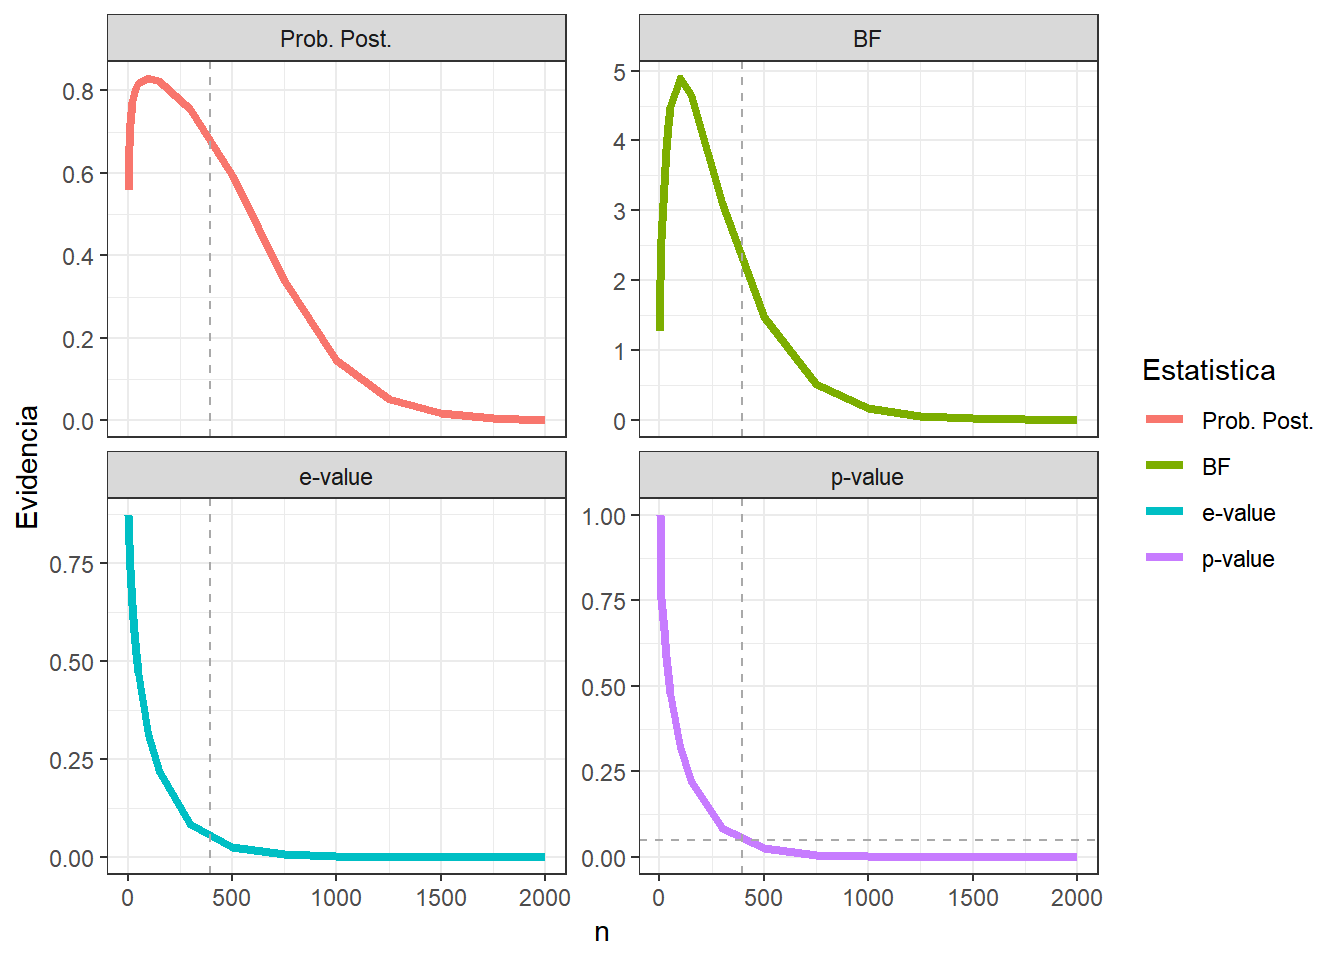
\includegraphics[width=0.8\linewidth]{InfBayes_files/figure-latex/unnamed-chunk-35-1} \end{center}

Note que quanto mais próximo \(M_x\) está de \(\theta_0\), menor a região \(T_x\) e, portanto, maior o valor da evidência em favor de \(H_0\). O valor da evidência pode ser calculado por

\(Ev(\Theta_0,x)=\) \(1-P\left(\theta_0\leq \theta\leq2M-\theta_0|x\right)=\) \(1-P\left(\dfrac{\theta_0-M}{\sqrt V}\leq Z\leq \dfrac{2M-\theta_0-M}{\sqrt V}|x\right)=\) \(2\Phi\left(-\dfrac{|\theta_0-M|}{\sqrt V}\right)=\) \(2\Phi\left(-\dfrac{\left|\dfrac{{\sigma}_0^2m+nv^2\bar{x}}{{\sigma}_0^2+nv^2}-\theta_0\right|}{\dfrac{{\sigma}_0 v}{\sqrt{{\sigma}_0^2+nv^2}}}\right)=\) \(2\Phi\left(-\dfrac{\sqrt{{\sigma}_0^2+nv^2}}{{\sigma}_0 v}\dfrac{|{\sigma}_0^2(m-\theta_0)+nv^2(\bar x-\theta_0)|}{\sqrt{{\sigma}_0^2+nv^2}}\right)=\) \(2\Phi\left(-\dfrac{1}{\sqrt{{\sigma}_0^2+nv^2}}\left|\dfrac{{\sigma}_0}{v}(m-\theta_0)+\dfrac{\sqrt n v}{{\sigma}_0}(\bar x-\theta_0)\right|\right)=\) \(2\Phi\left(-\dfrac{1}{\sqrt{{\sigma}_0^2+nv^2}}\left|\dfrac{(m-\theta_0)}{v/{\sigma}_0}+\sqrt nv\dfrac{(\bar x-\theta_0)}{{\sigma}_0/\sqrt n}\right|\right)\)

\(~\)

Sob a abordagem frequentista, temos que o \emph{p-value} é

\(p(\boldsymbol x)\)
\(= 1-P\left(-\dfrac{|\bar X-\theta_0|}{{\sigma}_0/\sqrt n}\leq Z \leq \dfrac{|\bar X-\theta_0|}{{\sigma}_0/\sqrt n}\right)\)
\(=2\Phi\left(-\dfrac{|\bar X-\theta_0|}{{\sigma}_0/\sqrt n}\right)\)
\(\Longleftrightarrow -\dfrac{|\bar X-\theta_0|}{{\sigma}_0/\sqrt n}=\Phi^{-1}\left(\dfrac{p-valor}{2}\right)\),

de modo que, nesse exemplo, podemos escrever

\(Ev(\Theta_0,x)=\) \(2\Phi\left(-\dfrac{1}{\sqrt{{\sigma}_0^2+nv^2}}~\left|\dfrac{(m-\theta_0)}{v/{\sigma}_0}+\sqrt nv~\Phi\left(\dfrac{p(\boldsymbol x)}{2}\right)\right|\right)\).

A seguir, são apresentados gráficos do \emph{e-value} e do \emph{p-value} como função de \(\bar{x}\) e do \emph{e-value} como função do \emph{p-value} usando da relação anterior.

\begin{center}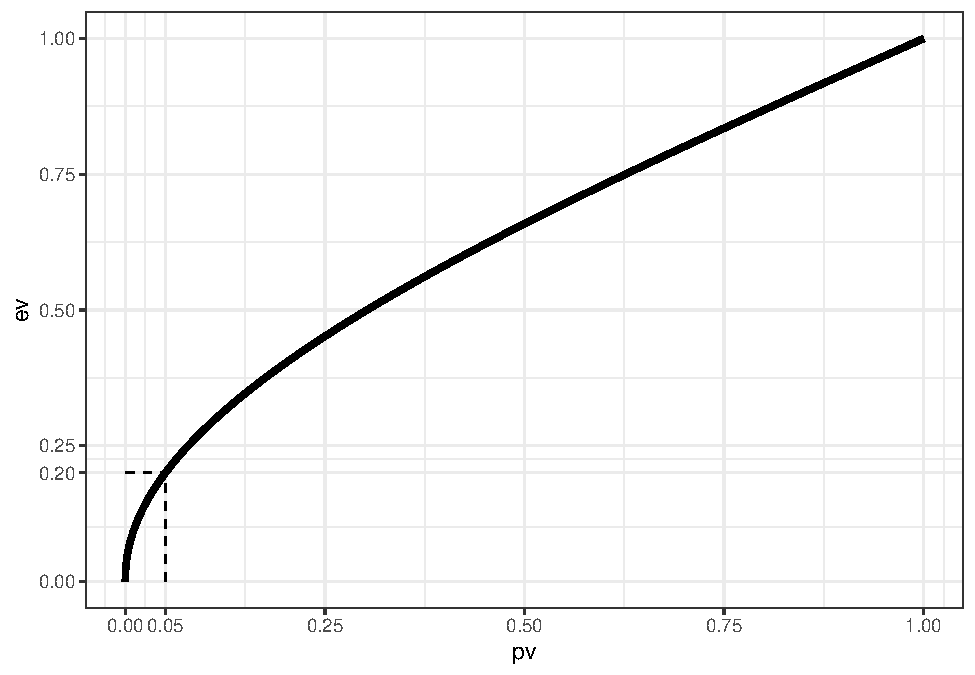
\includegraphics[width=0.8\linewidth]{InfBayes_files/figure-latex/unnamed-chunk-36-1} \end{center}

\begin{Shaded}
\begin{Highlighting}[]
\NormalTok{sigma02=}\DecValTok{4}
\NormalTok{m=}\DecValTok{0}\NormalTok{; v2=}\DecValTok{1}
\NormalTok{theta0 =}\StringTok{ }\DecValTok{0}
\NormalTok{n=}\DecValTok{3}
\NormalTok{p=}\KeywordTok{seq}\NormalTok{(}\DecValTok{0}\NormalTok{,}\DecValTok{1}\NormalTok{,}\DataTypeTok{length.out=}\DecValTok{5000}\NormalTok{)}
\NormalTok{ep =}\StringTok{  }\ControlFlowTok{function}\NormalTok{(p)\{}
  \DecValTok{2}\OperatorTok{*}\KeywordTok{pnorm}\NormalTok{(}\OperatorTok{-}\KeywordTok{abs}\NormalTok{(}\KeywordTok{sqrt}\NormalTok{(sigma02}\OperatorTok{/}\NormalTok{v2)}\OperatorTok{*}\NormalTok{(m}\OperatorTok{-}\NormalTok{theta0) }\OperatorTok{+}\StringTok{ }\KeywordTok{sqrt}\NormalTok{(n}\OperatorTok{*}\NormalTok{v2)}\OperatorTok{*}\KeywordTok{qnorm}\NormalTok{(p}\OperatorTok{/}\DecValTok{2}\NormalTok{))}\OperatorTok{/}\StringTok{ }\KeywordTok{sqrt}\NormalTok{(sigma02}\OperatorTok{+}\NormalTok{n}\OperatorTok{*}\NormalTok{v2))}
\NormalTok{\}}
\NormalTok{graf=}\KeywordTok{tibble}\NormalTok{(}\DataTypeTok{pv=}\NormalTok{p,}\DataTypeTok{ev=}\KeywordTok{ep}\NormalTok{(p)) }\OperatorTok
\StringTok{  }\KeywordTok{ggplot}\NormalTok{() }\OperatorTok{+}
\StringTok{  }\KeywordTok{geom_line}\NormalTok{(}\KeywordTok{aes}\NormalTok{(}\DataTypeTok{x=}\NormalTok{pv,}\DataTypeTok{y=}\NormalTok{ev),}\DataTypeTok{lwd=}\FloatTok{1.5}\NormalTok{) }\OperatorTok{+}
\StringTok{  }\KeywordTok{geom_segment}\NormalTok{(}\DataTypeTok{x=}\FloatTok{0.05}\NormalTok{,}\DataTypeTok{xend=}\FloatTok{0.05}\NormalTok{,}\DataTypeTok{y=}\DecValTok{0}\NormalTok{,}\DataTypeTok{yend=}\KeywordTok{round}\NormalTok{(}\KeywordTok{ep}\NormalTok{(}\FloatTok{0.05}\NormalTok{),}\DecValTok{2}\NormalTok{),}\DataTypeTok{lty=}\DecValTok{2}\NormalTok{) }\OperatorTok{+}
\StringTok{  }\KeywordTok{geom_segment}\NormalTok{(}\DataTypeTok{x=}\DecValTok{0}\NormalTok{,}\DataTypeTok{xend=}\FloatTok{0.05}\NormalTok{,}\DataTypeTok{y=}\KeywordTok{round}\NormalTok{(}\KeywordTok{ep}\NormalTok{(}\FloatTok{0.05}\NormalTok{),}\DecValTok{2}\NormalTok{),}\DataTypeTok{yend=}\KeywordTok{round}\NormalTok{(}\KeywordTok{ep}\NormalTok{(}\FloatTok{0.05}\NormalTok{),}\DecValTok{2}\NormalTok{),}\DataTypeTok{lty=}\DecValTok{2}\NormalTok{) }\OperatorTok{+}
\StringTok{  }\KeywordTok{scale_y_continuous}\NormalTok{(}\DataTypeTok{breaks=}\KeywordTok{c}\NormalTok{(}\FloatTok{0.00}\NormalTok{,}\KeywordTok{round}\NormalTok{(}\KeywordTok{ep}\NormalTok{(}\FloatTok{0.05}\NormalTok{),}\DecValTok{2}\NormalTok{),}\FloatTok{0.25}\NormalTok{,}\FloatTok{0.50}\NormalTok{,}\FloatTok{0.75}\NormalTok{,}\FloatTok{1.00}\NormalTok{)) }\OperatorTok{+}
\StringTok{  }\KeywordTok{scale_x_continuous}\NormalTok{(}\DataTypeTok{breaks=}\KeywordTok{c}\NormalTok{(}\FloatTok{0.00}\NormalTok{,}\FloatTok{0.05}\NormalTok{,}\FloatTok{0.25}\NormalTok{,}\FloatTok{0.50}\NormalTok{,}\FloatTok{0.75}\NormalTok{,}\FloatTok{1.00}\NormalTok{)) }\OperatorTok{+}
\StringTok{  }\KeywordTok{theme_bw}\NormalTok{()}
\ControlFlowTok{if}\NormalTok{(knitr}\OperatorTok{::}\KeywordTok{is_latex_output}\NormalTok{())\{}
\NormalTok{  graf}
\NormalTok{\} }\ControlFlowTok{else}\NormalTok{ \{ plotly}\OperatorTok{::}\KeywordTok{ggplotly}\NormalTok{(graf) \}}
\end{Highlighting}
\end{Shaded}

\begin{center}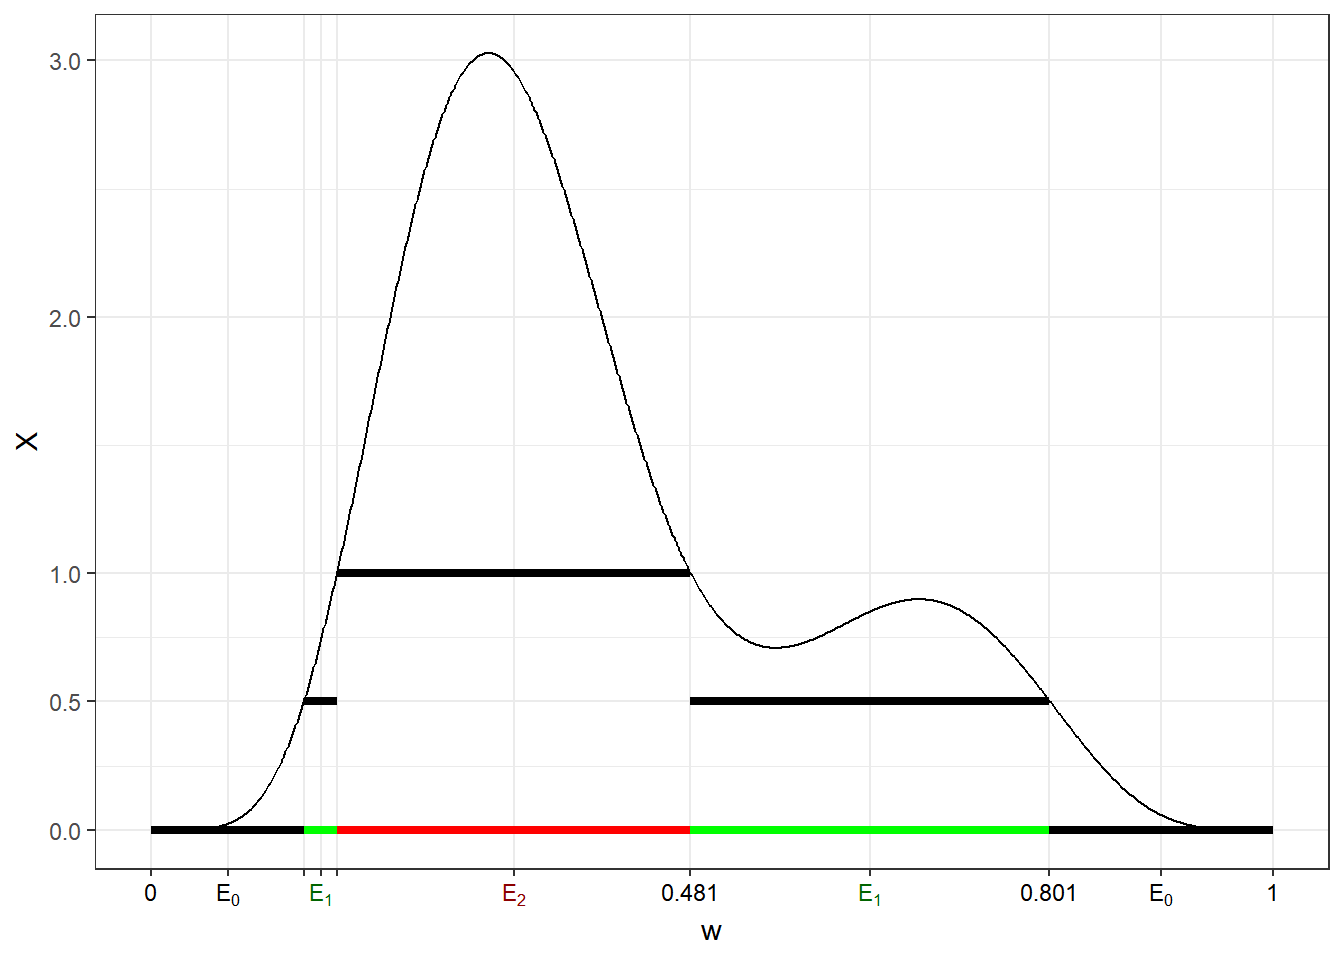
\includegraphics[width=0.8\linewidth]{InfBayes_files/figure-latex/unnamed-chunk-37-1} \end{center}

Suponha que um estatístico frequentista decida rejeitar \(H_0\) se o \emph{p-value} for menor que \emph{0.05}. Para que a decisão baseada no \emph{e-value} concorde com o resultado frequentista (para esse particular exemplo), deve-se rejeitar a hipótese se o \emph{e-value} for menor que \emph{0.2}, aproximadamente. Quando a variância da priori ou o tamanho amostral aumentam, os valores dessas duas medidas se aproximam.

\(~\)

\textbf{Resultados Assintóticos} (para esse exemplo)

Suponha que \(H_0: \theta=\theta_0\) seja falso, isto é, o ``verdadeiro'' valor do parâmetro é \(\theta^* \neq \theta_0\). Quando \(n\uparrow\infty\), pela Lei dos Grandes Números,

\(\bar{X} ~\overset{q.c.}{\longrightarrow}~ \theta^*\)
\(~\Longrightarrow~ \dfrac{\sqrt{n}|\bar{X}-\theta_0|}{{\sigma}_0} ~{\longrightarrow}~ +\infty\)
\(~\Longrightarrow~ p(\boldsymbol X)= 2\Phi\left(-\dfrac{\sqrt{n}|\bar{X}-\theta_0|}{{\sigma}_0}\right) ~{\longrightarrow}~ 0\),

com probabilidade 1. Por outro lado, sob \(H_0: \theta=\theta_0\), pelo Teorema Central do Limite,

\(\dfrac{\sqrt{n}(\bar{X}-\theta_0)}{{\sigma}_0} ~\overset{\mathcal{D}}\longrightarrow~ Z \sim N(0,1)\)
\(~\Longrightarrow~ p(\boldsymbol X)= 2\Phi\left(-\dfrac{\sqrt{n}|\bar{X}-\theta_0|}{{\sigma}_0}\right) ~\overset{\mathcal{D}}\longrightarrow~ U=2\Phi\left(-|Z|\right) \sim Unif(0,1)\).

\(~\)

Esses resultados para o \emph{p-value} são bastante conhecidos. No contexto desse exemplo, é possível obter resultados similares para o \emph{e-value}. Novamente, considere que \(H_0\) é falso e, sem perda de generalidade, \(\theta=\theta^*>\theta_0\). Note que

\(\dfrac{{\sigma}_0(m-\theta_0)}{v\sqrt{{\sigma}_0^2+nv^2}} ~\longrightarrow~ 0\)

e, pela LGN,

\(\bar{X} ~\overset{q.c.}{\longrightarrow}~ \theta^*\)
\(~\Longrightarrow~ (\bar{X}-\theta_0) ~{\longrightarrow}~ (\theta^*-\theta_0) >0\)
\(~\Longrightarrow~ \dfrac{nv(\bar{X}-\theta_0)}{{\sigma}_0^2\sqrt{{\sigma}_0^2+nv^2}} ~{\longrightarrow}~ +\infty\)
\(~\Longrightarrow~ Ev(\Theta_0,\boldsymbol X)=2\Phi\left(-\left|\dfrac{{\sigma}_0(m-\theta_0)}{v{\sqrt{{\sigma}_0^2+nv^2}}}+\dfrac{nv(\bar x-\theta_0)}{{\sigma}_0{\sqrt{{\sigma}_0^2+nv^2}}}\right|\right) ~{\longrightarrow}~ 2\Phi\left(-\infty\right)=0\).

Além disso, \(\dfrac{v\sqrt{n}}{\sqrt{{\sigma}_0^2+nv^2}} ~\longrightarrow~ 1\) e, sob \(H_0: \theta = \theta_0\),

\(\dfrac{v\sqrt{n}}{\sqrt{{\sigma}_0^2+nv^2}}\dfrac{\sqrt{n}(\bar{X}-\theta_0)}{{\sigma}_0} ~\overset{\mathcal{D}}\longrightarrow~ Z \sim N(0,1)\),

de modo que

\(Ev(\Theta_0,\boldsymbol{X})=2\Phi\left(-\left|\dfrac{{\sigma}_0(m-\theta_0)}{v{\sqrt{{\sigma}_0^2+nv^2}}}+\dfrac{nv(\bar x-\theta_0)}{{\sigma}_0{\sqrt{{\sigma}_0^2+nv^2}}}\right|\right) ~{\longrightarrow}~ 2\Phi\left(-|Z|\right)\sim Unif(0,1)\).

Esse resultado pode não valer em outros contextos. Por exemplo, quando \(dim(\Theta_0)\geq 2\), a distribuição de \(Ev(\Theta_0,\boldsymbol{X})\) sob \(H_0\) não é \(Unif(0,1)\), em geral.

\(~\)

\(~\)

\hypertarget{p-value---nivel-de-significuxe2ncia-adaptativo}{%
\section{P-value - Nivel de Significância Adaptativo}\label{p-value---nivel-de-significuxe2ncia-adaptativo}}

Recentemente, o \emph{p-value} e a utilização do famoso nível \(\alpha=0.05\) têm sido muito questionados, não apenas na área de testes de hipóteses mas na ciência como um todo. A ideia de fixar um nível de significância é que a probabilidade de \emph{erro tipo I} fica ``controlada'' e a probabilidade do \emph{erro tipo II} diminui quanto maior o tamanho amostral. Por essa razão, é comum nas áreas de planejamento de experimentos e amostragem, o cálculo do tamanho amostral para um determinado estudo. Infelizmente, na maior parte dos problemas do dia a dia de um estatístico, não há um planejamento cuidadoso ou as amostras disponíveis são ``amostras de conveniência''. Simultaneamente, com a ``revolução da informação'', a quantidade de dados disponível é cada vez maior. A consequência disso no cenário de testes de hipóteses é que os testes ficam muito poderosos e há uma tendência maior de rejeitar a hipótese nula.

\(~\)

\textbf{Exemplo.} Seja \(X_1,\ldots,X_n\) c.i.i.d. tais que \(X_i|\theta \sim Ber(\theta)\), \(\theta \sim Beta(a,b)\) de modo que \(\theta|x=\sum x_i \sim Beta(a+x,b+n-x)\) e suponha que deseja-se testar \(H_0: \theta= 1/2\). A seguir, para diferentes tamanhos amostrais \(n\) e supondo que em todos os casos \(\bar{x}_n=0.55\), são apresentados os testes para esse caso vistos até aqui: \emph{p-value} do teste RVG, probabilidade posterior e \(BF\) do teste de Jeffreys e \emph{e-value} do FBST.

\begin{Shaded}
\begin{Highlighting}[]
\NormalTok{a=}\DecValTok{1}\NormalTok{; b=}\DecValTok{1}
\NormalTok{p=}\FloatTok{0.5}
\NormalTok{alpha=}\FloatTok{0.05}
\NormalTok{theta0=}\FloatTok{0.5}
\NormalTok{xbar=}\FloatTok{0.55}
\NormalTok{N=}\KeywordTok{c}\NormalTok{(}\DecValTok{1}\NormalTok{,}\DecValTok{5}\NormalTok{,}\DecValTok{10}\NormalTok{,}\DecValTok{20}\NormalTok{,}\DecValTok{30}\NormalTok{,}\DecValTok{40}\NormalTok{,}\DecValTok{50}\NormalTok{,}\DecValTok{100}\NormalTok{,}\DecValTok{150}\NormalTok{,}\DecValTok{300}\NormalTok{,}\KeywordTok{seq}\NormalTok{(}\DecValTok{500}\NormalTok{,}\DecValTok{2000}\NormalTok{,}\DecValTok{250}\NormalTok{))}
\NormalTok{p_v=}\KeywordTok{Vectorize}\NormalTok{(}\ControlFlowTok{function}\NormalTok{(n)\{}
\NormalTok{  x=n}\OperatorTok{*}\NormalTok{xbar}
\NormalTok{  l =}\StringTok{ }\KeywordTok{c}\NormalTok{(}\KeywordTok{min}\NormalTok{(x,n}\OperatorTok{-}\NormalTok{x),}\KeywordTok{max}\NormalTok{(x,n}\OperatorTok{-}\NormalTok{x))}
  \KeywordTok{pbinom}\NormalTok{(l[}\DecValTok{1}\NormalTok{],n,theta0) }\OperatorTok{+}\StringTok{ }\DecValTok{1}\OperatorTok{-}\KeywordTok{pbinom}\NormalTok{(l[}\DecValTok{2}\NormalTok{],n,theta0) \})}
\NormalTok{Nalpha=}\KeywordTok{seq}\NormalTok{(}\KeywordTok{max}\NormalTok{(N[(}\KeywordTok{p_v}\NormalTok{(N)}\OperatorTok{-}\NormalTok{alpha)}\OperatorTok{>}\DecValTok{0}\NormalTok{]),}\KeywordTok{min}\NormalTok{(N[(}\KeywordTok{p_v}\NormalTok{(N)}\OperatorTok{-}\NormalTok{alpha)}\OperatorTok{<}\DecValTok{0}\NormalTok{]))}
\NormalTok{Nalpha=Nalpha[}\KeywordTok{which.min}\NormalTok{(}\KeywordTok{abs}\NormalTok{(}\KeywordTok{p_v}\NormalTok{(Nalpha)}\OperatorTok{-}\NormalTok{alpha))]}
\NormalTok{bf=}\KeywordTok{Vectorize}\NormalTok{(}\ControlFlowTok{function}\NormalTok{(n)\{}
\NormalTok{  x=n}\OperatorTok{*}\NormalTok{xbar}
  \CommentTok{# exp(log(BF))}
  \KeywordTok{exp}\NormalTok{(x}\OperatorTok{*}\KeywordTok{log}\NormalTok{(theta0) }\OperatorTok{+}\StringTok{ }\NormalTok{(n}\OperatorTok{-}\NormalTok{x)}\OperatorTok{*}\KeywordTok{log}\NormalTok{(}\DecValTok{1}\OperatorTok{-}\NormalTok{theta0) }\OperatorTok{+}\StringTok{ }\KeywordTok{lbeta}\NormalTok{(a,b) }\OperatorTok{-}\StringTok{ }\KeywordTok{lbeta}\NormalTok{(a}\OperatorTok{+}\NormalTok{x,b}\OperatorTok{+}\NormalTok{n}\OperatorTok{-}\NormalTok{x)) \})}
\NormalTok{prob_post=}\KeywordTok{Vectorize}\NormalTok{(}\ControlFlowTok{function}\NormalTok{(n)\{}
\NormalTok{  x=n}\OperatorTok{*}\NormalTok{xbar}
\NormalTok{  l =}\StringTok{ }\KeywordTok{log}\NormalTok{(}\DecValTok{1}\OperatorTok{-}\NormalTok{p)}\OperatorTok{+}\KeywordTok{lbeta}\NormalTok{(a}\OperatorTok{+}\NormalTok{x,b}\OperatorTok{+}\NormalTok{n}\OperatorTok{-}\NormalTok{x)}\OperatorTok{-}\KeywordTok{log}\NormalTok{(p)}\OperatorTok{-}\NormalTok{x}\OperatorTok{*}\KeywordTok{log}\NormalTok{(theta0)}\OperatorTok{-}\NormalTok{(n}\OperatorTok{-}\NormalTok{x)}\OperatorTok{*}\KeywordTok{log}\NormalTok{(}\DecValTok{1}\OperatorTok{-}\NormalTok{theta0)}\OperatorTok{-}\KeywordTok{lbeta}\NormalTok{(a,b)}
  \DecValTok{1}\OperatorTok{/}\NormalTok{(}\DecValTok{1}\OperatorTok{+}\KeywordTok{exp}\NormalTok{(l)) \})}
\NormalTok{e_v=}\KeywordTok{Vectorize}\NormalTok{(}\ControlFlowTok{function}\NormalTok{(n)\{}
\NormalTok{  x=n}\OperatorTok{*}\NormalTok{xbar}
\NormalTok{  f_Tx=}\ControlFlowTok{function}\NormalTok{(t)\{ }\KeywordTok{dbeta}\NormalTok{(t,a}\OperatorTok{+}\NormalTok{x,b}\OperatorTok{+}\NormalTok{n}\OperatorTok{-}\NormalTok{x)}\OperatorTok{-}\KeywordTok{dbeta}\NormalTok{(theta0,a}\OperatorTok{+}\NormalTok{x,b}\OperatorTok{+}\NormalTok{n}\OperatorTok{-}\NormalTok{x) \}}
\NormalTok{  moda=(a}\OperatorTok{+}\NormalTok{x}\DecValTok{-1}\NormalTok{)}\OperatorTok{/}\NormalTok{(a}\OperatorTok{+}\NormalTok{b}\OperatorTok{+}\NormalTok{n}\DecValTok{-2}\NormalTok{)}
  \ControlFlowTok{if}\NormalTok{(theta0}\OperatorTok{==}\NormalTok{moda)\{ }\KeywordTok{return}\NormalTok{(}\DecValTok{1}\NormalTok{) \}}
  \ControlFlowTok{if}\NormalTok{(theta0}\OperatorTok{<}\NormalTok{moda)\{}
\NormalTok{    Tx=}\KeywordTok{c}\NormalTok{(theta0,}\KeywordTok{uniroot}\NormalTok{(}\DataTypeTok{f=}\NormalTok{f_Tx,}\DataTypeTok{lower=}\NormalTok{moda,}\DataTypeTok{upper=}\DecValTok{1}\NormalTok{)}\OperatorTok{$}\NormalTok{root)}
\NormalTok{  \}}\ControlFlowTok{else}\NormalTok{\{}
\NormalTok{    Tx=}\KeywordTok{c}\NormalTok{(}\KeywordTok{uniroot}\NormalTok{(}\DataTypeTok{f=}\NormalTok{f_Tx,}\DataTypeTok{lower=}\DecValTok{0}\NormalTok{,}\DataTypeTok{upper=}\NormalTok{moda)}\OperatorTok{$}\NormalTok{root,theta0)}
\NormalTok{  \}}
  \KeywordTok{pbeta}\NormalTok{(Tx[}\DecValTok{1}\NormalTok{],a}\OperatorTok{+}\NormalTok{x,b}\OperatorTok{+}\NormalTok{n}\OperatorTok{-}\NormalTok{x)}\OperatorTok{+}\DecValTok{1}\OperatorTok{-}\KeywordTok{pbeta}\NormalTok{(Tx[}\DecValTok{2}\NormalTok{],a}\OperatorTok{+}\NormalTok{x,b}\OperatorTok{+}\NormalTok{n}\OperatorTok{-}\NormalTok{x)}
\NormalTok{\})}
\NormalTok{Dados=}\KeywordTok{tibble}\NormalTok{(}\DataTypeTok{n=}\KeywordTok{rep}\NormalTok{(N,}\DecValTok{4}\NormalTok{), }\DataTypeTok{Evidencia=}\KeywordTok{c}\NormalTok{(}\KeywordTok{p_v}\NormalTok{(N),}\KeywordTok{prob_post}\NormalTok{(N),}\KeywordTok{bf}\NormalTok{(N),}\KeywordTok{e_v}\NormalTok{(N)),}
       \DataTypeTok{Estatistica=}\KeywordTok{factor}\NormalTok{(}\KeywordTok{rep}\NormalTok{(}\KeywordTok{c}\NormalTok{(}\StringTok{"p-value"}\NormalTok{,}\StringTok{"Prob. Post."}\NormalTok{,}\StringTok{"BF"}\NormalTok{,}\StringTok{"e-value"}\NormalTok{),}
          \DataTypeTok{each=}\KeywordTok{length}\NormalTok{(N)),}\DataTypeTok{levels=}\KeywordTok{c}\NormalTok{(}\StringTok{"Prob. Post."}\NormalTok{,}\StringTok{"BF"}\NormalTok{,}\StringTok{"e-value"}\NormalTok{,}\StringTok{"p-value"}\NormalTok{)),}
       \DataTypeTok{corte=}\KeywordTok{c}\NormalTok{(}\KeywordTok{p_v}\NormalTok{(Nalpha),}\KeywordTok{rep}\NormalTok{(}\OtherTok{NA}\NormalTok{,}\DecValTok{4}\OperatorTok{*}\KeywordTok{length}\NormalTok{(N)}\OperatorTok{-}\DecValTok{1}\NormalTok{)))}
\KeywordTok{ggplot}\NormalTok{(Dados)}\OperatorTok{+}
\StringTok{  }\KeywordTok{geom_line}\NormalTok{(}\KeywordTok{aes}\NormalTok{(}\DataTypeTok{x=}\NormalTok{n,}\DataTypeTok{y=}\NormalTok{Evidencia, }\DataTypeTok{colour=}\NormalTok{Estatistica),}\DataTypeTok{lwd=}\FloatTok{1.5}\NormalTok{)}\OperatorTok{+}
\StringTok{  }\KeywordTok{geom_vline}\NormalTok{(}\DataTypeTok{xintercept=}\NormalTok{Nalpha,}\DataTypeTok{lty=}\DecValTok{2}\NormalTok{,}\DataTypeTok{col=}\StringTok{"darkgrey"}\NormalTok{)}\OperatorTok{+}
\StringTok{  }\KeywordTok{facet_wrap}\NormalTok{(}\OperatorTok{~}\NormalTok{Estatistica, }\DataTypeTok{scales=}\StringTok{"free_y"}\NormalTok{)}\OperatorTok{+}
\StringTok{  }\KeywordTok{geom_hline}\NormalTok{(}\DataTypeTok{data=}\KeywordTok{subset}\NormalTok{(Dados,Estatí}\DataTypeTok{stica=}\StringTok{"p-value"}\NormalTok{),}\KeywordTok{aes}\NormalTok{(}\DataTypeTok{yintercept=}\NormalTok{corte), }\DataTypeTok{lty=}\DecValTok{2}\NormalTok{, }\DataTypeTok{col=}\StringTok{"darkgrey"}\NormalTok{)}\OperatorTok{+}
\StringTok{  }\KeywordTok{theme_bw}\NormalTok{()}
\end{Highlighting}
\end{Shaded}

\begin{center}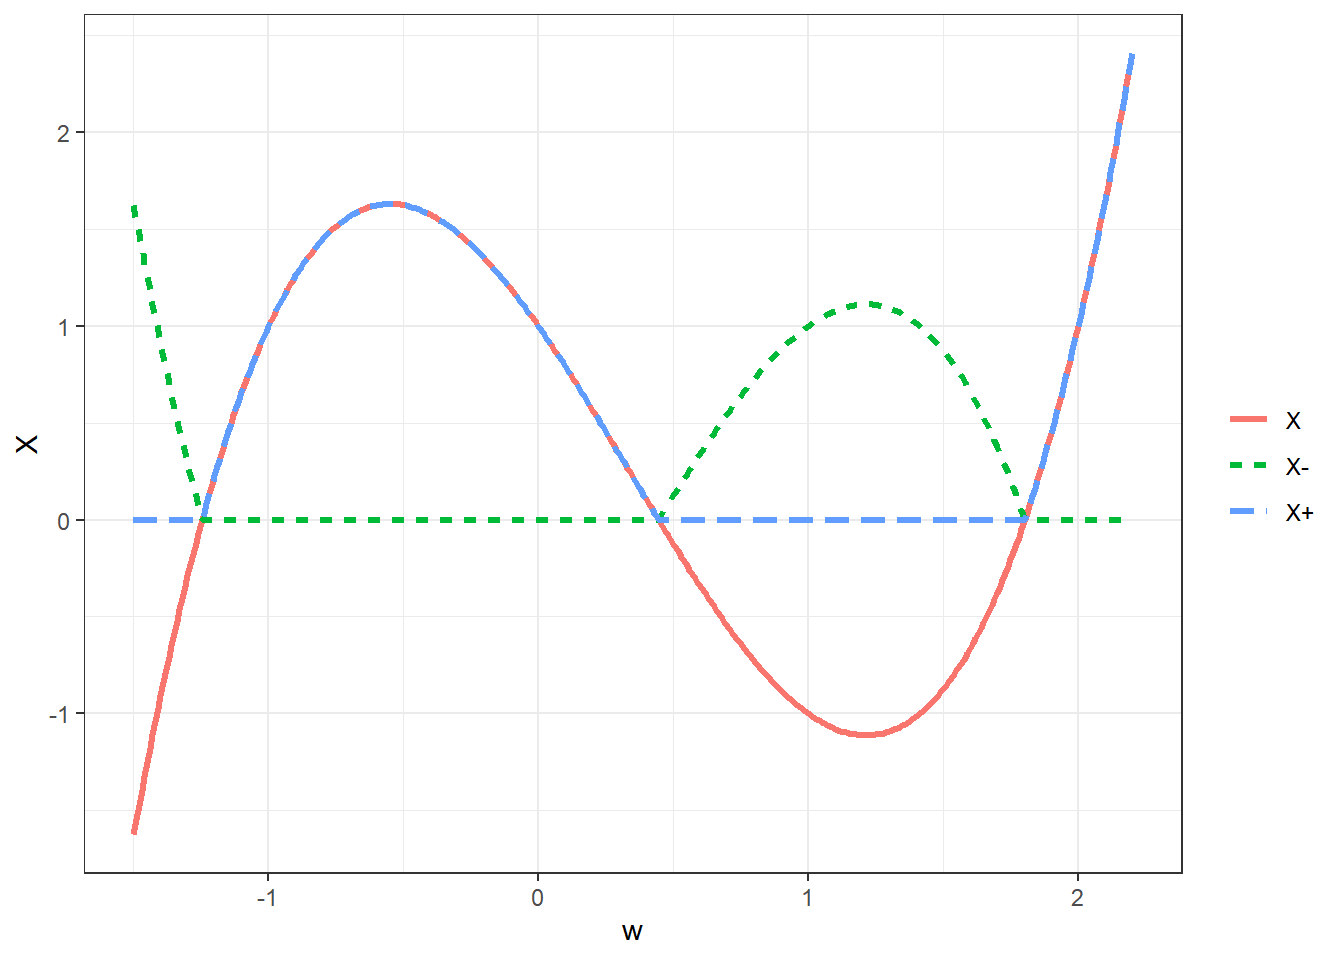
\includegraphics[width=0.8\linewidth]{InfBayes_files/figure-latex/unnamed-chunk-38-1} \end{center}

Note que todas as medidas de suporte da hipótese tendem a zero conforme aumenta o tamanho amostral. Isso indica que se \(|\bar{x}_n-\theta_0|=\varepsilon\) e for fixado um valor de corte para essas medidas que não dependa do tamanho amostral (por exemplo, o \(\alpha=0.05\) para o \emph{p-value}), existe um \(n^*\) tal que \(H_0\) será rejeitado para todo \(n\geq n^*\). No gráfico, a linha vertical tracejada indica o valor \(n^*\) para o \emph{p-value} considerando o corte \(\alpha=0.05\).

\(~\)

Como visto anteriormente, o Lema de Neyman-Pearson Generalizado (DeGroot, 1986) garante que os testes Bayesianos (baseados na probabilidade posterior ou no BF) minimizam \(a\alpha + b\beta\). Baseado nesse resultado, O professor Carlos A. B. Pereira recentemente propôs um novo procedimento de teste para evitar o problema descrito anteriormente.

\begin{enumerate}
\def\labelenumi{\arabic{enumi}.}
\item
  Seja \(BF(\boldsymbol x) = \dfrac{f_0(\boldsymbol x)}{f_1(\boldsymbol x)}\)
  \(=\dfrac{\displaystyle\int_{\Theta_0} f(\boldsymbol x|\theta) dP_0(\theta)}{\displaystyle \int_{\Theta_1} f(\boldsymbol x|\theta) dP_1(\theta)}\), onde \(P_i\) é a medida de probabilidade a priori para \(\theta\) restrito à hipótese \(H_i\), \(i=0,1\);
\item
  Defina
  \(\alpha_n = P\left(\left\{\boldsymbol x : BF(\boldsymbol x)\leq\dfrac{b}{a}\right\} ~\Big|~ \Theta_0\right)\) e
  \(\beta_n = P\left(\left\{\boldsymbol x : BF(\boldsymbol x)>\dfrac{b}{a}\right\} ~\Big|~ \Theta_1\right)\);
\item
  Suponha que foi observado \(\boldsymbol X=\boldsymbol x_o\). O \textbf{P-value} é dado por
  \(\text{P-value}(\boldsymbol x_o) = P\left(\left\{\boldsymbol x : BF(\boldsymbol x)\leq BF(\boldsymbol x_o)\right\} ~\Big|~ \Theta_0\right)\);
\item
  O procedimento de teste consiste em rejeitar \(H_0\) se \(\text{P-value}(\boldsymbol x) < \alpha_n\).
\end{enumerate}

\(~\)

\textbf{Voltando ao Exemplo.} As distribuções preditivas sob \(H_0: \theta=\theta_0=1/2\) e \(H_1:\theta \neq 1/2\) são

\(f_0(\boldsymbol x)\) \(= f(\boldsymbol x | \theta_0)\)
\(=\displaystyle \binom{n}{x} {\theta}_0^x (1-{\theta}_0)^{n-x}\)
\(=\displaystyle \binom{n}{x} {(1/2)^{n}}\) ;

\(f_1(\boldsymbol x)\)
\(=\displaystyle \int_{\Theta\setminus\theta_0} f(\boldsymbol x|\theta) f(\theta) d\theta\)
\(=\displaystyle \int_0^1 \binom{n}{x} \dfrac{{\theta}_0^{a+x-1} (1-{\theta}_0)^{b+n-x-1}}{\beta(a,b)}~d\theta\)
\(=\displaystyle \binom{n}{x}\dfrac{\beta(a+x,b+n-x)}{\beta(a,b)}\) .

Deste modo,

\(BF(\boldsymbol x)\) \(=\dfrac{f_0(\boldsymbol x)}{f_1(\boldsymbol x)}\)
\(=\dfrac{\beta(a,b)~{\theta}_0^x (1-{\theta}_0)^{n-x}}{\beta(a+x,b+n-x)}\)
\(=\dfrac{\beta(a,b)~(1/2)^{n}}{\beta(a+x,b+n-x)}\),

e, assim,

\(\alpha_n = \displaystyle {(1/2)^{n}} \sum_{\left\{\boldsymbol x: BF(\boldsymbol x)\leq\frac{b}{a}\right\}}\binom{n}{x}\),

\(\beta_n = \displaystyle \dfrac{1}{{\beta(a,b)}} \sum_{\left\{\boldsymbol x: BF(\boldsymbol x)>\frac{b}{a}\right\}}\binom{n}{x}\beta(a+x,b+n-x)\),

\(\text{P-value}(\boldsymbol x_0) = \displaystyle {(1/2)^{n}} \sum_{\left\{\boldsymbol x: BF(\boldsymbol x)\leq BF(\boldsymbol x_o)\right\}}\binom{n}{x}\)

\(~\)

Supondo novamente que foi observado \(\bar{x}=0.55\), o gráfico abaixo apresenta esses valores para diversos tamanhos amostrais.

\begin{Shaded}
\begin{Highlighting}[]
\NormalTok{a=}\DecValTok{1}\NormalTok{; b=}\DecValTok{1}
\NormalTok{a1=}\DecValTok{1}\NormalTok{; b1=}\DecValTok{1}
\NormalTok{p=}\FloatTok{0.5}
\NormalTok{alpha=}\FloatTok{0.05}
\NormalTok{theta0=}\FloatTok{0.5}
\NormalTok{xbar=}\FloatTok{0.55}
\NormalTok{N=}\KeywordTok{c}\NormalTok{(}\DecValTok{2}\NormalTok{,}\DecValTok{5}\NormalTok{,}\KeywordTok{seq}\NormalTok{(}\DecValTok{10}\NormalTok{,}\DecValTok{150}\NormalTok{,}\DecValTok{10}\NormalTok{),}\KeywordTok{seq}\NormalTok{(}\DecValTok{150}\NormalTok{,}\DecValTok{1000}\NormalTok{,}\DecValTok{50}\NormalTok{))}
\NormalTok{bf=}\KeywordTok{Vectorize}\NormalTok{(}\ControlFlowTok{function}\NormalTok{(x,n)\{}
  \KeywordTok{exp}\NormalTok{(x}\OperatorTok{*}\KeywordTok{log}\NormalTok{(theta0) }\OperatorTok{+}\StringTok{ }\NormalTok{(n}\OperatorTok{-}\NormalTok{x)}\OperatorTok{*}\KeywordTok{log}\NormalTok{(}\DecValTok{1}\OperatorTok{-}\NormalTok{theta0) }\OperatorTok{+}\StringTok{ }\KeywordTok{lbeta}\NormalTok{(a,b) }\OperatorTok{-}\StringTok{ }\KeywordTok{lbeta}\NormalTok{(a}\OperatorTok{+}\NormalTok{x,b}\OperatorTok{+}\NormalTok{n}\OperatorTok{-}\NormalTok{x))}
\NormalTok{\}, }\DataTypeTok{vectorize.args =} \KeywordTok{c}\NormalTok{(}\StringTok{"x"}\NormalTok{))}
\NormalTok{alphaN =}\StringTok{ }\KeywordTok{Vectorize}\NormalTok{(}\ControlFlowTok{function}\NormalTok{(n)\{}
\NormalTok{  x=n}\OperatorTok{*}\NormalTok{xbar}
\NormalTok{  s=}\KeywordTok{seq}\NormalTok{(}\DecValTok{0}\NormalTok{,n)}
\NormalTok{  s=s[}\KeywordTok{bf}\NormalTok{(s,n)}\OperatorTok{<=}\NormalTok{b1}\OperatorTok{/}\NormalTok{a1]}
\NormalTok{  (}\FloatTok{0.5}\NormalTok{)}\OperatorTok{^}\NormalTok{n}\OperatorTok{*}\KeywordTok{sum}\NormalTok{(}\KeywordTok{choose}\NormalTok{(n,s))}
\NormalTok{\})}
\NormalTok{betaN =}\StringTok{ }\KeywordTok{Vectorize}\NormalTok{(}\ControlFlowTok{function}\NormalTok{(n)\{}
\NormalTok{  x=n}\OperatorTok{*}\NormalTok{xbar}
\NormalTok{  s=}\KeywordTok{seq}\NormalTok{(}\DecValTok{0}\NormalTok{,n)}
\NormalTok{  s=s[}\KeywordTok{bf}\NormalTok{(s,n)}\OperatorTok{>}\NormalTok{b1}\OperatorTok{/}\NormalTok{a1]}
  \KeywordTok{sum}\NormalTok{(extraDistr}\OperatorTok{::}\KeywordTok{dbbinom}\NormalTok{(s,n,a,b))}
\NormalTok{\})}
\NormalTok{P_v=}\KeywordTok{Vectorize}\NormalTok{(}\ControlFlowTok{function}\NormalTok{(n)\{}
\NormalTok{  x=n}\OperatorTok{*}\NormalTok{xbar}
\NormalTok{  s=}\KeywordTok{seq}\NormalTok{(}\DecValTok{0}\NormalTok{,n)}
\NormalTok{  s=s[}\KeywordTok{bf}\NormalTok{(s,n)}\OperatorTok{<=}\KeywordTok{bf}\NormalTok{(x,n)]}
\NormalTok{  (}\FloatTok{0.5}\NormalTok{)}\OperatorTok{^}\NormalTok{n}\OperatorTok{*}\KeywordTok{sum}\NormalTok{(}\KeywordTok{choose}\NormalTok{(n,s))}
\NormalTok{\})}
\NormalTok{Dados=}\KeywordTok{tibble}\NormalTok{(}\DataTypeTok{n=}\NormalTok{N, }\DataTypeTok{alpha=}\KeywordTok{alphaN}\NormalTok{(N), }\DataTypeTok{beta=}\KeywordTok{betaN}\NormalTok{(N), }\DataTypeTok{Pvalue=}\KeywordTok{P_v}\NormalTok{(N))}
\KeywordTok{ggplot}\NormalTok{(Dados)}\OperatorTok{+}
\StringTok{  }\KeywordTok{geom_line}\NormalTok{(}\KeywordTok{aes}\NormalTok{(}\DataTypeTok{x=}\NormalTok{n,}\DataTypeTok{y=}\NormalTok{Pvalue, }\DataTypeTok{colour=}\StringTok{"P-value"}\NormalTok{),}\DataTypeTok{lwd=}\FloatTok{1.2}\NormalTok{)}\OperatorTok{+}
\StringTok{  }\KeywordTok{geom_line}\NormalTok{(}\KeywordTok{aes}\NormalTok{(}\DataTypeTok{x=}\NormalTok{n,}\DataTypeTok{y=}\NormalTok{alpha, }\DataTypeTok{colour=}\StringTok{"alpha"}\NormalTok{),}\DataTypeTok{lwd=}\FloatTok{1.2}\NormalTok{)}\OperatorTok{+}
\StringTok{  }\KeywordTok{geom_line}\NormalTok{(}\KeywordTok{aes}\NormalTok{(}\DataTypeTok{x=}\NormalTok{n,}\DataTypeTok{y=}\NormalTok{beta, }\DataTypeTok{colour=}\StringTok{"beta"}\NormalTok{),}\DataTypeTok{lwd=}\FloatTok{1.2}\NormalTok{)}\OperatorTok{+}
\StringTok{  }\KeywordTok{geom_line}\NormalTok{(}\KeywordTok{aes}\NormalTok{(}\DataTypeTok{x=}\NormalTok{n,}\DataTypeTok{y=}\NormalTok{alpha}\OperatorTok{+}\NormalTok{beta, }\DataTypeTok{colour=}\StringTok{"alpha+beta"}\NormalTok{),}\DataTypeTok{lwd=}\FloatTok{1.2}\NormalTok{)}\OperatorTok{+}
\StringTok{  }\KeywordTok{theme_bw}\NormalTok{() }\OperatorTok{+}\StringTok{ }\KeywordTok{labs}\NormalTok{(}\DataTypeTok{colour=}\StringTok{""}\NormalTok{)}
\end{Highlighting}
\end{Shaded}

\begin{center}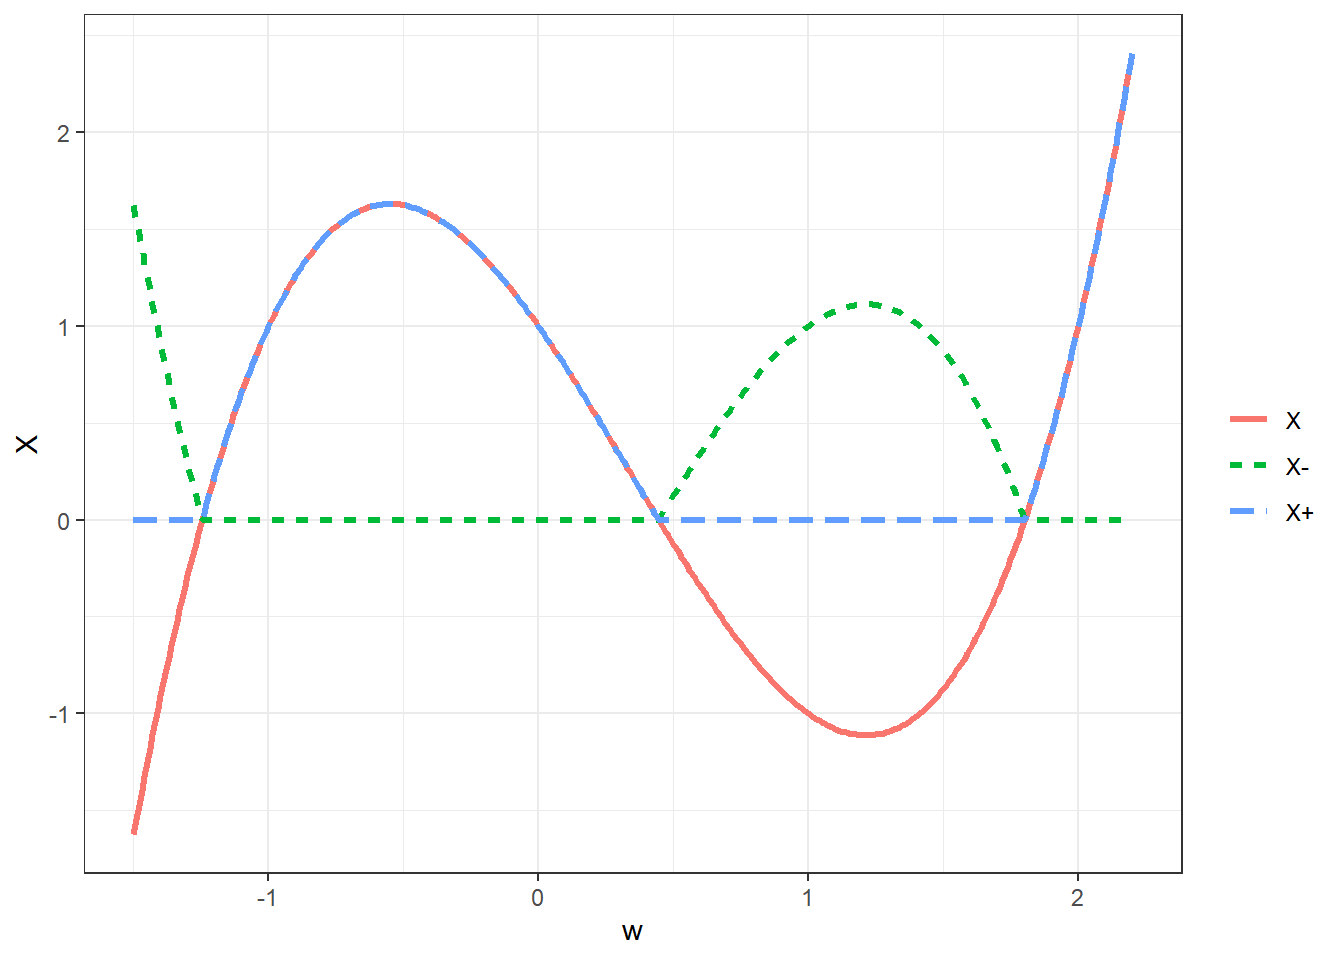
\includegraphics[width=0.8\linewidth]{InfBayes_files/figure-latex/unnamed-chunk-39-1} \end{center}

\(~\)

\(~\)

\hypertarget{Comp}{%
\chapter{Métodos Computacionais}\label{Comp}}

Como visto, a inferência Bayesiana é baseada na aplicação monótona do teorema de Bayes

\(f(\theta|\boldsymbol x)=\dfrac{f(\boldsymbol x|\theta)f(\theta)}{\displaystyle\int_\Theta f(\boldsymbol x|\theta)f(\theta)d\theta}\) \(= c(\boldsymbol x) f(\boldsymbol x|\theta)f(\theta)\) \(\propto f(\boldsymbol x|\theta)f(\theta)\),

e na obtenção de medidas resumo dessa distribuição, como \(E[\theta|\boldsymbol x]\), regiões HPD ou probabilidades a posteriori.

A maior dificuldade na aplicação de Inferência Bayesiana está justamente no cálculo das integrais envolvidas, tanto no cálculo de \(f(\boldsymbol x)\) para a obtenção da posteriori, quanto na obtenção das medidas resumos citadas anteriormente. Devido a isso, a inferência bayesiana ganhou muito força com o avanço computacional das últimas décadas. A seguir, serão apresentados um breve resumo de alguns recursos que podem ser utilizados na prática Bayesiana.

Muitos dos métodos descritos baseiam-se na \emph{Lei dos Grande Números} (LGN) e são uma bela aplicação de ideias frequentistas em um cenário controlado onde as suposições de \emph{i.i.d.} são satisfeitas.

\(~\)

\textbf{Lei \(\overset{\textbf{(Fraca)}}{\textbf{Forte}}\) dos Grande Números.} Seja \(X_1,X_2...\) uma sequência de v.a. i.i.d com \(E[X_1]=\mu\) e \(Var[X_1]=\sigma^2<\infty\), então

\(\dfrac{1}{n}\displaystyle \sum_{i=1}^n X_i ~~\underset{q.c.}{\overset{P}{\longrightarrow}}~~ E[X_1]=\mu\).

\(~\)

As integrais de interesse aqui serão escritas como o valor esperado de funções de variáveis aleatórias, isto é,

\(\displaystyle \int g(x) dP(x) = E\left[g(X)\right]\).

Deste modo, suponha que \(X_1,X_2...\) é uma sequência de v.a. i.i.d e \(g:\mathbb{R} \longrightarrow\mathbb{R}\) é uma função (mensurável) tal que \(Var\left[g(X_1)\right]<\infty\). Então, pela \emph{LGN},

\(\dfrac{1}{n}\displaystyle \sum_{i=1}^n g(X_i) ~\longrightarrow~ E\left[g(X_1)\right]\)

\(~\)

\hypertarget{muxe9todo-de-monte-carlo}{%
\section{Método de Monte Carlo}\label{muxe9todo-de-monte-carlo}}

Suponha que deseja-se calcular \(\displaystyle\int_\Theta g(\theta)f(\theta|\boldsymbol x)d\theta=E\left[g(\theta|\boldsymbol x)\right]\) e é possível simular realizações \(\theta_1,...,\theta_m\) da distribuição de \(\theta |\boldsymbol X=\boldsymbol x\) , \(f(\theta | \boldsymbol x)\).

Então, a integral acima pode ser aproximada por \(\displaystyle \dfrac{1}{m}\sum_{i=1}^m g(\theta_i)\)

\begin{itemize}
\tightlist
\item
  A precisão da aproximação é usualmente estimada pelo erro padrão da estimativa\\
  \(\displaystyle EP\left[\dfrac{1}{m}\sum_{i=1}^m g(\theta_i)\right]\)
  \(\approx \displaystyle \sqrt{\dfrac{1}{m}\left(\dfrac{1}{m}\sum_{i=1}^m\Big[g(\theta_i)\Big]^2-\left[\dfrac{1}{m}\sum_{j=1}^mg(\theta_j)\right]^2\right)}\)
\end{itemize}

\(~\)

\begin{quote}
\textbf{Exemplo 1.} Suponha que deseja-se estimar o número \(\pi\) usando o método de Monte Carlo. Considere então que o v.a. \((X,Y)\) tem distribuição uniforme em um quadrado centrado na origem, \(\mathfrak{X}=[-1,1]\times[-1,1]\), e um círculo \(A\) de raio \(1\) inscrito nesse quadrado, \(x^2+y^2\leq 1.\) Como a distribuição é uniforme no quadrado, a probabilidade de escolher um ponto no círculo é\\
\(P(A)\) \(=\dfrac{\text{área da círculo}}{\text{área do quadrado}}\) \(=\dfrac{\pi}{4}\) \(= \displaystyle\int_A f(x,y) dxdy\) \(= \displaystyle\int_{\mathfrak{X}} \mathbb{I}_A(x,y)~\dfrac{1}{4}~dxdy\) \(=E\left[\mathbb{I}_A(X,Y)\right]~.\)\\
Suponha que é possível gerar uma amostra \(\left\{(x_1,y_1),\ldots,(x_m,y_m)\right\}\) de \((X,Y)\), de modo que podemos aproximar o valor de \(\pi\) por\\
\(\pi\) \(=4~P(A)\) \(=E\left[4~\mathbb{I}_A(X,Y)\right]\) \(\displaystyle \approx \dfrac{1}{m}\sum_{i=1}^m 4~\mathbb{I}_A(x_i,y_i)\),\\
e, denotando por \(\displaystyle t=\sum_{i=1}^m ~\mathbb{I}_A(x_i,y_i)\), o erro estimado é\\
\(\displaystyle \sqrt{\dfrac{1}{m}\left(\dfrac{1}{m}\sum_{i=1}^m\Big[4~\mathbb{I}(x_i,y_i)\Big]^2-\left[\dfrac{1}{m}\sum_{j=1}^m 4~\mathbb{I}(x_i,y_i)\right]^2\right)}\)
\(=\displaystyle \sqrt{\dfrac{1}{m}\left(\dfrac{16}{m}~t-\left[\dfrac{4}{m}~t\right]^2\right)}\)
\(= \displaystyle \sqrt{\dfrac{16}{m} \dfrac{t}{m}\left(1-\dfrac{t}{m}\right)}\)
\(\leq \displaystyle \sqrt{\dfrac{16}{m}~\dfrac{1}{4}}\)
\(= \dfrac{2}{\sqrt{m}}~.\)
\end{quote}

\begin{Shaded}
\begin{Highlighting}[]
\KeywordTok{set.seed}\NormalTok{(}\DecValTok{666}\NormalTok{)}
\NormalTok{M =}\StringTok{ }\DecValTok{1000} \CommentTok{# número de iterações}
\NormalTok{df =}\StringTok{ }\KeywordTok{tibble}\NormalTok{(}\DataTypeTok{t =} \DecValTok{1}\OperatorTok{:}\NormalTok{M, }\DataTypeTok{x =} \KeywordTok{runif}\NormalTok{(}\KeywordTok{length}\NormalTok{(t), }\DecValTok{-1}\NormalTok{, }\DecValTok{1}\NormalTok{), }
            \DataTypeTok{y =} \KeywordTok{runif}\NormalTok{(}\KeywordTok{length}\NormalTok{(t), }\DecValTok{-1}\NormalTok{, }\DecValTok{1}\NormalTok{)) }\OperatorTok\StringTok{ }
\StringTok{  }\KeywordTok{mutate}\NormalTok{(}\DataTypeTok{Circ=}\KeywordTok{ifelse}\NormalTok{(x}\OperatorTok{^}\DecValTok{2}\OperatorTok{+}\NormalTok{y}\OperatorTok{^}\DecValTok{2}\OperatorTok{<=}\DecValTok{1}\NormalTok{,}\DecValTok{1}\NormalTok{,}\DecValTok{0}\NormalTok{), }
         \DataTypeTok{pi_est=}\KeywordTok{round}\NormalTok{(}\DecValTok{4}\OperatorTok{*}\KeywordTok{cumsum}\NormalTok{(Circ)}\OperatorTok{/}\NormalTok{t,}\DecValTok{4}\NormalTok{),}
         \DataTypeTok{erro=}\KeywordTok{round}\NormalTok{(}\KeywordTok{abs}\NormalTok{(pi}\OperatorTok{-}\NormalTok{pi_est),}\DecValTok{4}\NormalTok{),}
         \DataTypeTok{erro_est=}\KeywordTok{round}\NormalTok{(}\KeywordTok{sqrt}\NormalTok{((}\KeywordTok{cumsum}\NormalTok{(}\DecValTok{16}\OperatorTok{*}\NormalTok{Circ)}\OperatorTok{/}\NormalTok{t}\OperatorTok{-}\NormalTok{pi_est}\OperatorTok{^}\DecValTok{2}\NormalTok{)}\OperatorTok{/}\NormalTok{t),}\DecValTok{4}\NormalTok{))}
\NormalTok{p <-}\StringTok{ }\KeywordTok{ggplot}\NormalTok{() }\OperatorTok{+}\StringTok{ }\KeywordTok{theme_bw}\NormalTok{() }\OperatorTok{+}\StringTok{ }
\StringTok{        }\KeywordTok{theme}\NormalTok{(}\DataTypeTok{panel.grid.major =} \KeywordTok{element_blank}\NormalTok{(),}
            \DataTypeTok{panel.grid.minor =} \KeywordTok{element_blank}\NormalTok{(),}
            \DataTypeTok{panel.border =} \KeywordTok{element_blank}\NormalTok{(),}
            \DataTypeTok{panel.background =} \KeywordTok{element_blank}\NormalTok{()) }\OperatorTok{+}
\StringTok{        }\NormalTok{ggforce}\OperatorTok{::}\KeywordTok{geom_circle}\NormalTok{(}\KeywordTok{aes}\NormalTok{(}\DataTypeTok{x0 =} \DecValTok{0}\NormalTok{, }\DataTypeTok{y0 =} \DecValTok{0}\NormalTok{, }\DataTypeTok{r =} \DecValTok{1}\NormalTok{), }\DataTypeTok{color =} \StringTok{"black"}\NormalTok{) }\OperatorTok{+}
\StringTok{        }\KeywordTok{geom_rect}\NormalTok{(}\KeywordTok{aes}\NormalTok{(}\DataTypeTok{xmin =} \DecValTok{-1}\NormalTok{, }\DataTypeTok{ymin =} \DecValTok{-1}\NormalTok{, }\DataTypeTok{xmax =} \DecValTok{1}\NormalTok{, }\DataTypeTok{ymax =} \DecValTok{1}\NormalTok{), }
                  \DataTypeTok{color =} \StringTok{"black"}\NormalTok{, }\DataTypeTok{alpha =} \DecValTok{0}\NormalTok{) }\OperatorTok{+}\StringTok{ }
\StringTok{        }\KeywordTok{guides}\NormalTok{(}\DataTypeTok{color =} \OtherTok{FALSE}\NormalTok{) }\OperatorTok{+}
\StringTok{        }\KeywordTok{geom_point}\NormalTok{(}\DataTypeTok{data =}\NormalTok{ df, }\KeywordTok{aes}\NormalTok{(}\DataTypeTok{x =}\NormalTok{ x, }\DataTypeTok{y =}\NormalTok{ y, }\DataTypeTok{colour =}\NormalTok{ Circ), }\DataTypeTok{size =} \DecValTok{3}\NormalTok{)}
\NormalTok{p}\OperatorTok{+}\KeywordTok{labs}\NormalTok{(}\DataTypeTok{title =} \KeywordTok{expression}\NormalTok{(}\KeywordTok{paste}\NormalTok{(}\StringTok{"Método de Monte-Carlo para a estimação do "}\NormalTok{,pi)), }\DataTypeTok{subtitle =} \KeywordTok{paste}\NormalTok{(}\StringTok{"m = "}\NormalTok{,df}\OperatorTok{$}\NormalTok{t[M],}\StringTok{"  ;   pi_est = 4*("}\NormalTok{,}\KeywordTok{cumsum}\NormalTok{(df}\OperatorTok{$}\NormalTok{Circ)[M],}\StringTok{"/"}\NormalTok{,df}\OperatorTok{$}\NormalTok{t[M],}\StringTok{") = "}\NormalTok{,df}\OperatorTok{$}\NormalTok{pi_est[M],}\StringTok{"  ;   erro = "}\NormalTok{,df}\OperatorTok{$}\NormalTok{erro[M],}\StringTok{"  ;   erro_est = "}\NormalTok{,df}\OperatorTok{$}\NormalTok{erro_est[M]))}
\end{Highlighting}
\end{Shaded}

\begin{center}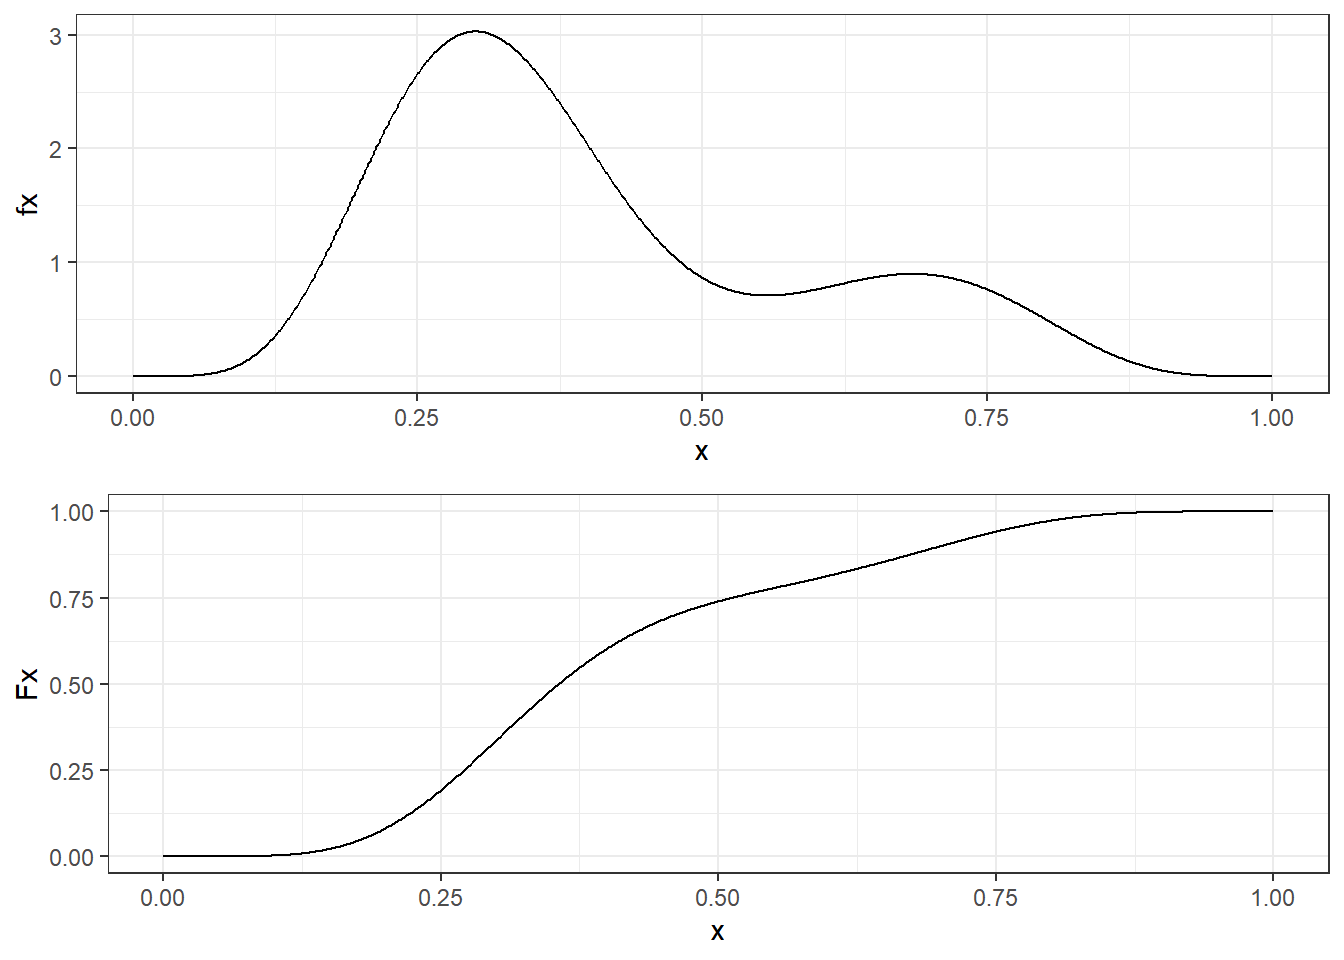
\includegraphics[width=0.8\linewidth]{InfBayes_files/figure-latex/unnamed-chunk-40-1} \end{center}

\begin{center}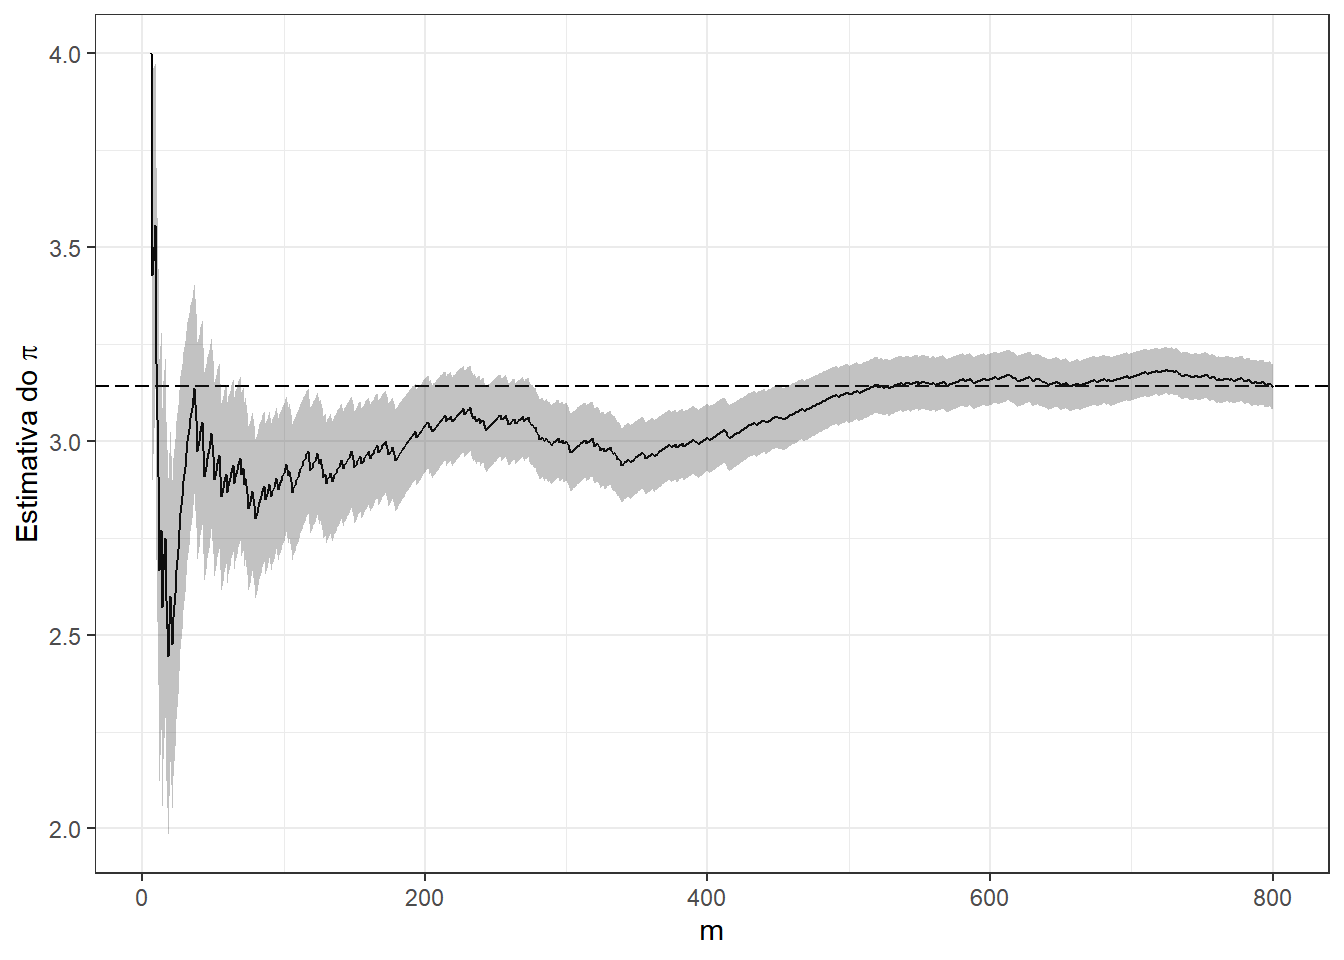
\includegraphics[width=0.8\linewidth]{InfBayes_files/figure-latex/unnamed-chunk-42-1} \end{center}

\begin{center}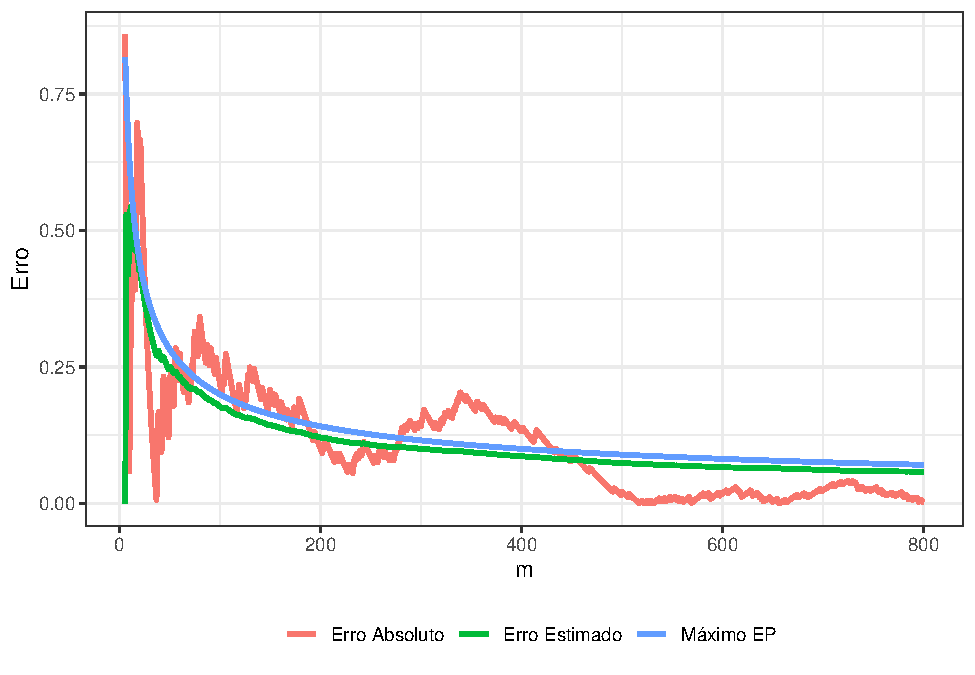
\includegraphics[width=0.8\linewidth]{InfBayes_files/figure-latex/unnamed-chunk-44-1} \end{center}

\(~\)

\begin{quote}
\textbf{Exemplo 2.} Suponha que você não sabe que
\[\displaystyle \int_0^1 x^3(1-x)^5e^xdx = 74046 - 27240e\approx0.0029928\]
e deseja estimar o resultado usando o método de Monte Carlo. Assim, considere as duas propostas a seguir\\
1. \(U \sim Unif (0,1)\) e a integral pode ser escrita como \(E\left[U^3(1-U)^5e^U\right]\);\\
2. \(Y \sim Beta(4,6)\) de modo que\\
\(\displaystyle \int_0^1 y^3(1-y)^5e^y dy\) \(=\beta(4,6)\displaystyle \int_0^1 e^y~~\frac{y^{4-1}(1-y)^{6-1}}{\beta(4,6)}~dy\) \(=\beta(4,6)E\left[e^Y\right]\).
\end{quote}

\begin{center}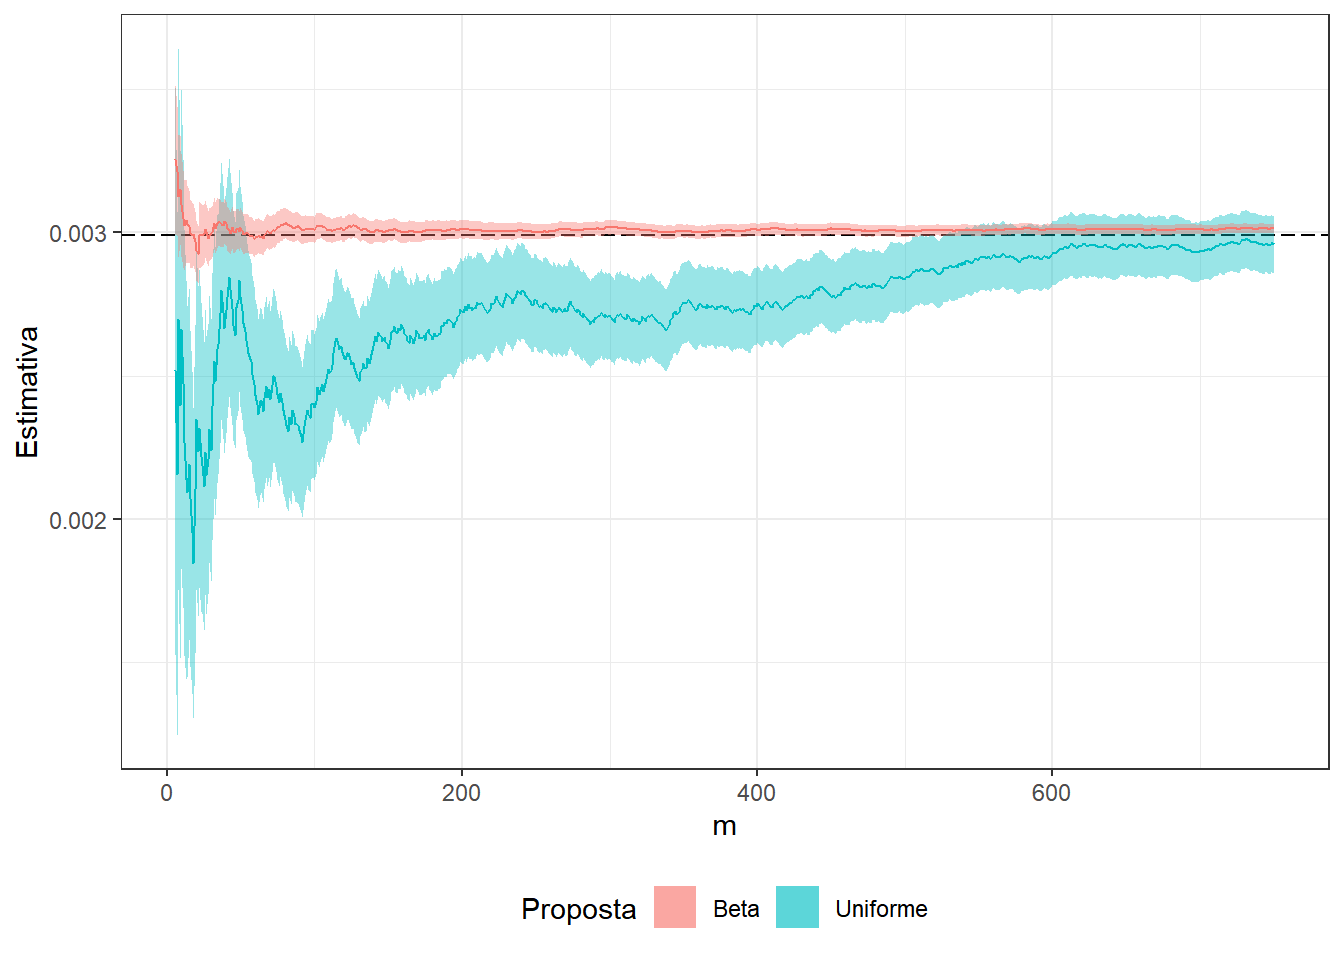
\includegraphics[width=0.8\linewidth]{InfBayes_files/figure-latex/unnamed-chunk-46-1} \end{center}

\begin{center}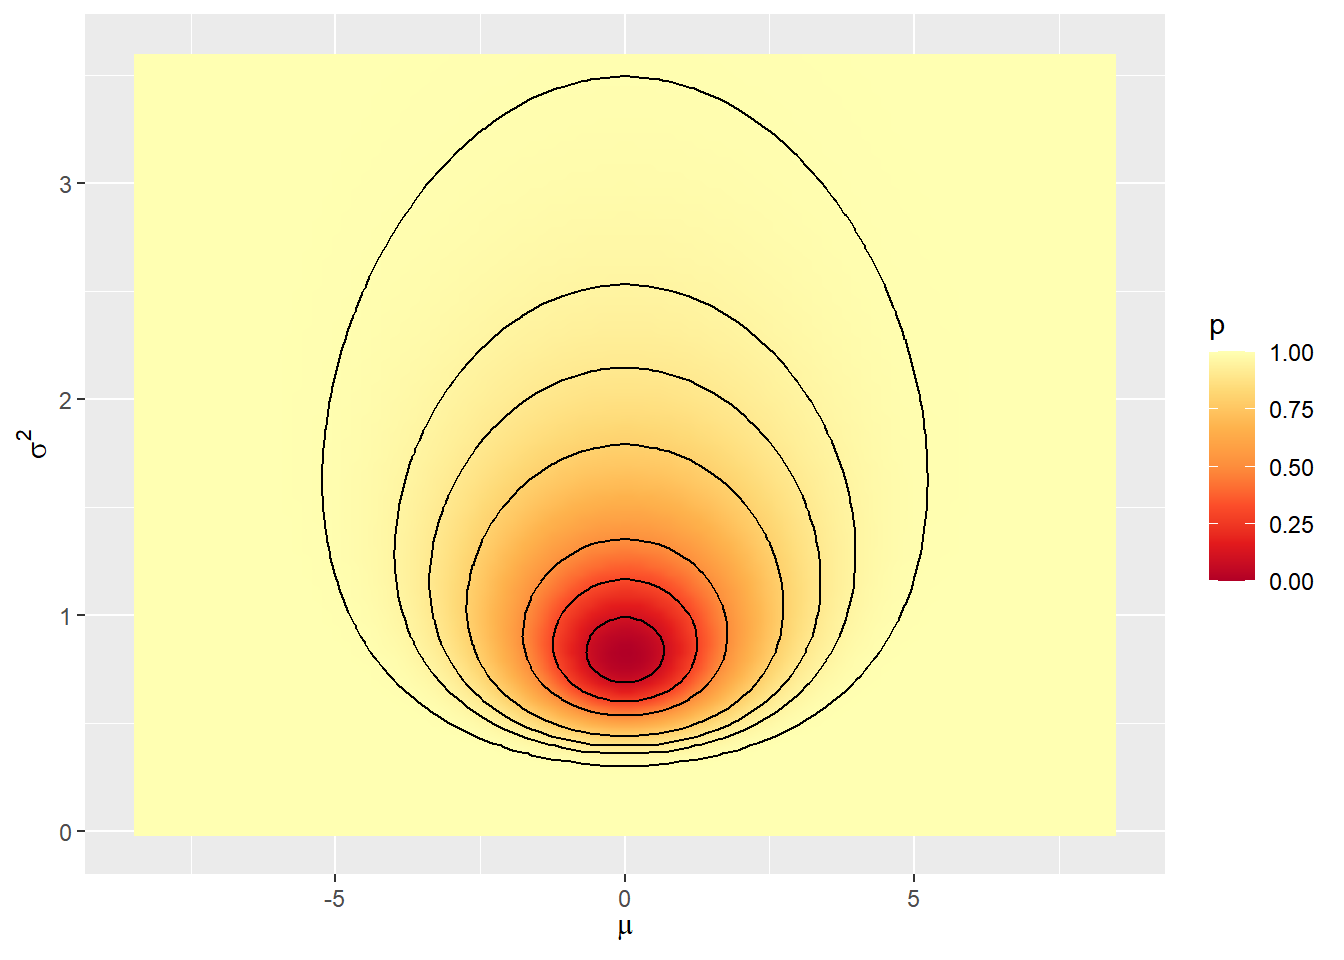
\includegraphics[width=0.8\linewidth]{InfBayes_files/figure-latex/unnamed-chunk-48-1} \end{center}

\(~\)

\begin{quote}
\textbf{Exemplo 3. Região HPD} Suponha que \(\boldsymbol \theta=(\mu,\sigma^2) \sim \textit{Normal-Inv.Gama}(m,v,a,b)\) e deseja-se obter estimativas pontuais e por região para \(\boldsymbol \theta\).\\
\(~\)\\
Se não houver um simulador da distribuição Normal-Inv.Gamma diretamente, é possível gerar um ponto \(\boldsymbol \theta_i=(\mu_i,\sigma_i)\) tomando \({\sigma}_i^2 \sim \textit{Inv.Gama}(a,b)\) (ou \(\tau_i \sim \textit{Gama}(a,b)\) e fazer \({\sigma}_i^2=1/\tau_i\)) e \(\mu_i \sim \textit{Normal}(m,{\sigma}_i^2/v)\). Nesse exemplo é fácil simular uma amostra da distribuição posterior e é possível obter estimativas pontuais simplesmente obtendo estatística resumo da amostra simulada, como média, moda, mediana, variância e desvio padrão.\\
\(~\)\\
Para construir a região HPD, primeiramente note que\\
\(R=\left\{\boldsymbol{\theta}\in\Theta :~f(\boldsymbol{\theta} | \boldsymbol{x})\geq h)\right\}=\left\{\boldsymbol{\theta}\in\Theta:~f(\boldsymbol x|\boldsymbol{\theta})f(\boldsymbol{\theta})\geq h^*=c\cdot h\right\}\),\\
de modo que não é necessário conhecer a constante \(c=f(\boldsymbol{x})\) para realizar essa tarefa. Como nesse exemplo a distribuição a posteriori é conhecida e fácil de ser simulada, considere o algorítmo a seguir para estimar a região HPD de probabilidade \(\gamma\).\\
\(~\)\\
1. Simular \(\boldsymbol{\theta}_1,...,\boldsymbol{\theta}_m\) de \(f(\boldsymbol{\theta}|\boldsymbol{x})\);\\
2. Encontrar \(h\) tal que \(\displaystyle \dfrac{1}{m}\sum_{i=1}^m\mathbb{I}_{R}(\boldsymbol{\theta}_i)=\dfrac{1}{m}\sum_{i=1}^m\mathbb{I}(f(\boldsymbol{\theta}_i|\boldsymbol{x})\geq h)\approx \gamma\)\\
\(~~~\) i. Calcule \(f(\boldsymbol{\theta}_i|\boldsymbol{x})\), \(i=1,\ldots,m\);\\
\(~~~\) ii. Ordene esses valores e tome \(h\) como o percentil de ordem \(\gamma\);\\
3. Fazer o gráfico da curva de nível \(f(\boldsymbol{\theta}|\boldsymbol{x})=h\).
\end{quote}

\begin{Shaded}
\begin{Highlighting}[]
\KeywordTok{set.seed}\NormalTok{(}\DecValTok{666}\NormalTok{)}
\NormalTok{a=}\DecValTok{7}\NormalTok{; b=}\DecValTok{7}\NormalTok{; m=}\DecValTok{0}\NormalTok{; v=}\FloatTok{0.5} \CommentTok{# parametros da posteriori}
\NormalTok{M=}\DecValTok{10000} \CommentTok{# No. de simulações}
\NormalTok{dpost=}\KeywordTok{Vectorize}\NormalTok{(}\ControlFlowTok{function}\NormalTok{(t1,t2)\{ }\CommentTok{#densidade posterior}
\NormalTok{  extraDistr}\OperatorTok{::}\KeywordTok{dinvgamma}\NormalTok{(t2,a,b)}\OperatorTok{*}\KeywordTok{dnorm}\NormalTok{(t1,m,}\KeywordTok{sqrt}\NormalTok{(t2}\OperatorTok{/}\NormalTok{v))\})}
\CommentTok{# simulações}
\NormalTok{df =}\StringTok{ }\KeywordTok{tibble}\NormalTok{(}\DataTypeTok{sigma2=}\NormalTok{extraDistr}\OperatorTok{::}\KeywordTok{rinvgamma}\NormalTok{(M,a,b)) }\OperatorTok\StringTok{  }
\StringTok{  }\KeywordTok{mutate}\NormalTok{(}\DataTypeTok{mu=}\KeywordTok{rnorm}\NormalTok{(M,m,}\KeywordTok{sqrt}\NormalTok{(sigma2}\OperatorTok{/}\NormalTok{v)))}
\CommentTok{#summarytools::dfSummary(df, graph.magnif = 0.75, valid.col = FALSE, na.col = FALSE)}
\NormalTok{summarytools}\OperatorTok{::}\KeywordTok{dfSummary}\NormalTok{(df, }\DataTypeTok{plain.ascii =} \OtherTok{FALSE}\NormalTok{, }\DataTypeTok{style =} \StringTok{"grid"}\NormalTok{, }
          \DataTypeTok{graph.magnif =} \FloatTok{0.75}\NormalTok{, }\DataTypeTok{valid.col =} \OtherTok{FALSE}\NormalTok{, }\DataTypeTok{na.col =} \OtherTok{FALSE}\NormalTok{, }
          \DataTypeTok{varnumbers =} \OtherTok{FALSE}\NormalTok{, }\DataTypeTok{headings =} \OtherTok{FALSE}\NormalTok{, }\DataTypeTok{tmp.img.dir =} \StringTok{"./tmp"}\NormalTok{)}
\end{Highlighting}
\end{Shaded}

\begin{longtable}[]{@{}llll@{}}
\toprule
\begin{minipage}[b]{0.12\columnwidth}\raggedright
Variable\strut
\end{minipage} & \begin{minipage}[b]{0.26\columnwidth}\raggedright
Stats / Values\strut
\end{minipage} & \begin{minipage}[b]{0.25\columnwidth}\raggedright
Freqs (\% of Valid)\strut
\end{minipage} & \begin{minipage}[b]{0.25\columnwidth}\raggedright
Graph\strut
\end{minipage}\tabularnewline
\midrule
\endhead
\begin{minipage}[t]{0.12\columnwidth}\raggedright
sigma2\\
{[}numeric{]}\strut
\end{minipage} & \begin{minipage}[t]{0.26\columnwidth}\raggedright
Mean (sd) : 1.2 (0.5)\\
min \textless{} med \textless{} max:\\
0.3 \textless{} 1.1 \textless{} 7.3\\
IQR (CV) : 0.6 (0.4)\strut
\end{minipage} & \begin{minipage}[t]{0.25\columnwidth}\raggedright
10000 distinct values\strut
\end{minipage} & \begin{minipage}[t]{0.25\columnwidth}\raggedright
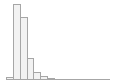
\includegraphics{./tmp/ds0023.png}\strut
\end{minipage}\tabularnewline
\begin{minipage}[t]{0.12\columnwidth}\raggedright
mu\\
{[}numeric{]}\strut
\end{minipage} & \begin{minipage}[t]{0.26\columnwidth}\raggedright
Mean (sd) : 0 (1.5)\\
min \textless{} med \textless{} max:\\
-7.3 \textless{} 0 \textless{} 6.1\\
IQR (CV) : 2 (-253.7)\strut
\end{minipage} & \begin{minipage}[t]{0.25\columnwidth}\raggedright
10000 distinct values\strut
\end{minipage} & \begin{minipage}[t]{0.25\columnwidth}\raggedright
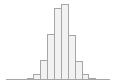
\includegraphics{./tmp/ds0024.png}\strut
\end{minipage}\tabularnewline
\bottomrule
\end{longtable}

\begin{Shaded}
\begin{Highlighting}[]
\NormalTok{df =}\StringTok{ }\NormalTok{df }\OperatorTok\StringTok{ }\KeywordTok{mutate}\NormalTok{(}\DataTypeTok{post=}\KeywordTok{dpost}\NormalTok{(mu,sigma2))}
\CommentTok{# variáveis para os gráficos}
\NormalTok{gama=}\KeywordTok{c}\NormalTok{(}\FloatTok{0.99}\NormalTok{,}\FloatTok{0.95}\NormalTok{,}\FloatTok{0.9}\NormalTok{,}\FloatTok{0.8}\NormalTok{,}\FloatTok{0.5}\NormalTok{,}\FloatTok{0.3}\NormalTok{,}\FloatTok{0.1}\NormalTok{) }\CommentTok{# prob das regiões}
\NormalTok{l=}\KeywordTok{quantile}\NormalTok{(df}\OperatorTok{$}\NormalTok{post,}\DecValTok{1}\OperatorTok{-}\NormalTok{gama)}
\NormalTok{d=}\DecValTok{100}
\NormalTok{x=}\KeywordTok{seq}\NormalTok{(}\OperatorTok{-}\DecValTok{4}\OperatorTok{*}\NormalTok{extraDistr}\OperatorTok{::}\KeywordTok{qinvgamma}\NormalTok{(}\FloatTok{0.5}\NormalTok{,a,b)}\OperatorTok{/}\NormalTok{v,}\DecValTok{4}\OperatorTok{*}\NormalTok{extraDistr}\OperatorTok{::}\KeywordTok{qinvgamma}\NormalTok{(}\FloatTok{0.5}\NormalTok{,a,b)}\OperatorTok{/}\NormalTok{v,}\DataTypeTok{length.out =}\NormalTok{ d)}
\NormalTok{y=}\KeywordTok{seq}\NormalTok{(}\DecValTok{0}\NormalTok{,extraDistr}\OperatorTok{::}\KeywordTok{qinvgamma}\NormalTok{(}\FloatTok{0.996}\NormalTok{,a,b),}\DataTypeTok{length.out =}\NormalTok{ d)}
\NormalTok{z=}\KeywordTok{matrix}\NormalTok{(}\KeywordTok{apply}\NormalTok{(}\KeywordTok{cbind}\NormalTok{(}\KeywordTok{rep}\NormalTok{(x,d),}\KeywordTok{rep}\NormalTok{(y,}\DataTypeTok{each=}\NormalTok{d)),}\DecValTok{1}\NormalTok{,}\ControlFlowTok{function}\NormalTok{(t)\{}\KeywordTok{dpost}\NormalTok{(t[}\DecValTok{1}\NormalTok{],t[}\DecValTok{2}\NormalTok{])\}),}\DataTypeTok{ncol=}\NormalTok{d)}
\CommentTok{# gráfico da posteriori}
\CommentTok{# Create a function interpolating colors in the range of specified colors}
\NormalTok{jet.colors <-}\StringTok{ }\KeywordTok{colorRampPalette}\NormalTok{(}\KeywordTok{c}\NormalTok{(}\StringTok{'green'}\NormalTok{,}\StringTok{'yellow'}\NormalTok{,}\StringTok{'orange'}\NormalTok{,}\StringTok{'red'}\NormalTok{,}\StringTok{'darkred'}\NormalTok{))}
\CommentTok{# Generate the desired number of colors from this palette}
\NormalTok{nbcol <-}\StringTok{ }\DecValTok{300}
\NormalTok{cores <-}\StringTok{ }\KeywordTok{jet.colors}\NormalTok{(nbcol)}
\CommentTok{# Compute the z-value at the facet centres}
\NormalTok{zfacet <-}\StringTok{ }\NormalTok{z[}\OperatorTok{-}\DecValTok{1}\NormalTok{, }\DecValTok{-1}\NormalTok{] }\OperatorTok{+}\StringTok{ }\NormalTok{z[}\OperatorTok{-}\DecValTok{1}\NormalTok{, }\OperatorTok{-}\KeywordTok{ncol}\NormalTok{(z)] }\OperatorTok{+}\StringTok{ }
\StringTok{          }\NormalTok{z[}\OperatorTok{-}\KeywordTok{nrow}\NormalTok{(z), }\DecValTok{-1}\NormalTok{] }\OperatorTok{+}\StringTok{ }\NormalTok{z[}\OperatorTok{-}\KeywordTok{nrow}\NormalTok{(z), }\OperatorTok{-}\KeywordTok{ncol}\NormalTok{(z)]}
\CommentTok{# Recode facet z-values into color indices}
\NormalTok{facetcol <-}\StringTok{ }\KeywordTok{cut}\NormalTok{(zfacet, nbcol)}
\KeywordTok{persp}\NormalTok{(x, y, z, }\DataTypeTok{col =}\NormalTok{ cores[facetcol],}\DataTypeTok{theta=}\DecValTok{150}\NormalTok{,}\DataTypeTok{phi=}\DecValTok{30}\NormalTok{,}\DataTypeTok{expand=}\FloatTok{0.75}\NormalTok{,}
      \DataTypeTok{ticktype=}\StringTok{"simple"}\NormalTok{, }\DataTypeTok{xlab=}\KeywordTok{expression}\NormalTok{(mu), }\DataTypeTok{ylab=}\KeywordTok{expression}\NormalTok{(tau),}
      \DataTypeTok{zlab=}\KeywordTok{expression}\NormalTok{(}\KeywordTok{f}\NormalTok{(mu,tau)),}\DataTypeTok{axes=}\OtherTok{TRUE}\NormalTok{,}\DataTypeTok{border=}\OtherTok{NA}\NormalTok{,}\DataTypeTok{shade=}\FloatTok{0.9}\NormalTok{)}
\end{Highlighting}
\end{Shaded}

\begin{center}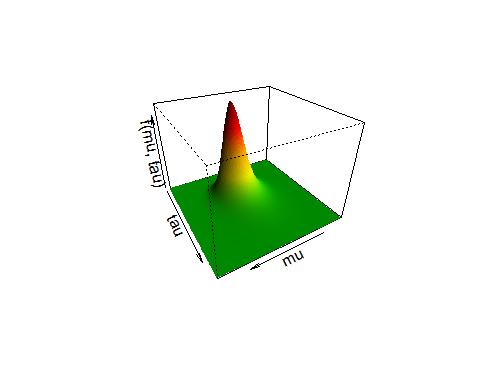
\includegraphics[width=0.8\linewidth]{InfBayes_files/figure-latex/unnamed-chunk-51-1} \end{center}

\begin{Shaded}
\begin{Highlighting}[]
\CommentTok{# gráfico das regiões HPD de prob. gama=c(0.99,0.95,0.9,0.8,0.5,0.3,0.1)}
\KeywordTok{tibble}\NormalTok{(}\DataTypeTok{x1=}\KeywordTok{rep}\NormalTok{(x,d),}\DataTypeTok{y1=}\KeywordTok{rep}\NormalTok{(y,}\DataTypeTok{each=}\NormalTok{d),}\DataTypeTok{z1=}\KeywordTok{as.vector}\NormalTok{(z)) }\OperatorTok
\StringTok{  }\KeywordTok{arrange}\NormalTok{(z1) }\OperatorTok\StringTok{ }\KeywordTok{mutate}\NormalTok{(}\DataTypeTok{p=}\DecValTok{1}\OperatorTok{-}\NormalTok{(}\KeywordTok{cumsum}\NormalTok{(z1)}\OperatorTok{/}\KeywordTok{sum}\NormalTok{(z1))) }\OperatorTok\StringTok{ }
\StringTok{  }\KeywordTok{ggplot}\NormalTok{(}\KeywordTok{aes}\NormalTok{(x1,y1,}\DataTypeTok{z=}\NormalTok{z1,}\DataTypeTok{fill =}\NormalTok{ p)) }\OperatorTok{+}
\StringTok{  }\KeywordTok{geom_raster}\NormalTok{(}\DataTypeTok{interpolate =} \OtherTok{TRUE}\NormalTok{) }\OperatorTok{+}
\StringTok{  }\NormalTok{jcolors}\OperatorTok{::}\KeywordTok{scale_fill_jcolors_contin}\NormalTok{(}\StringTok{"pal3"}\NormalTok{) }\OperatorTok{+}
\StringTok{  }\CommentTok{#scale_fill_distiller(palette = "YlOrRd") +}
\StringTok{  }\KeywordTok{geom_contour}\NormalTok{(}\DataTypeTok{breaks=}\NormalTok{l,}\DataTypeTok{col=}\StringTok{"black"}\NormalTok{) }\OperatorTok{+}
\StringTok{  }\KeywordTok{xlab}\NormalTok{(}\KeywordTok{expression}\NormalTok{(mu)) }\OperatorTok{+}\StringTok{ }\KeywordTok{ylab}\NormalTok{(}\KeywordTok{expression}\NormalTok{(sigma}\OperatorTok{^}\DecValTok{2}\NormalTok{))}
\end{Highlighting}
\end{Shaded}

\begin{center}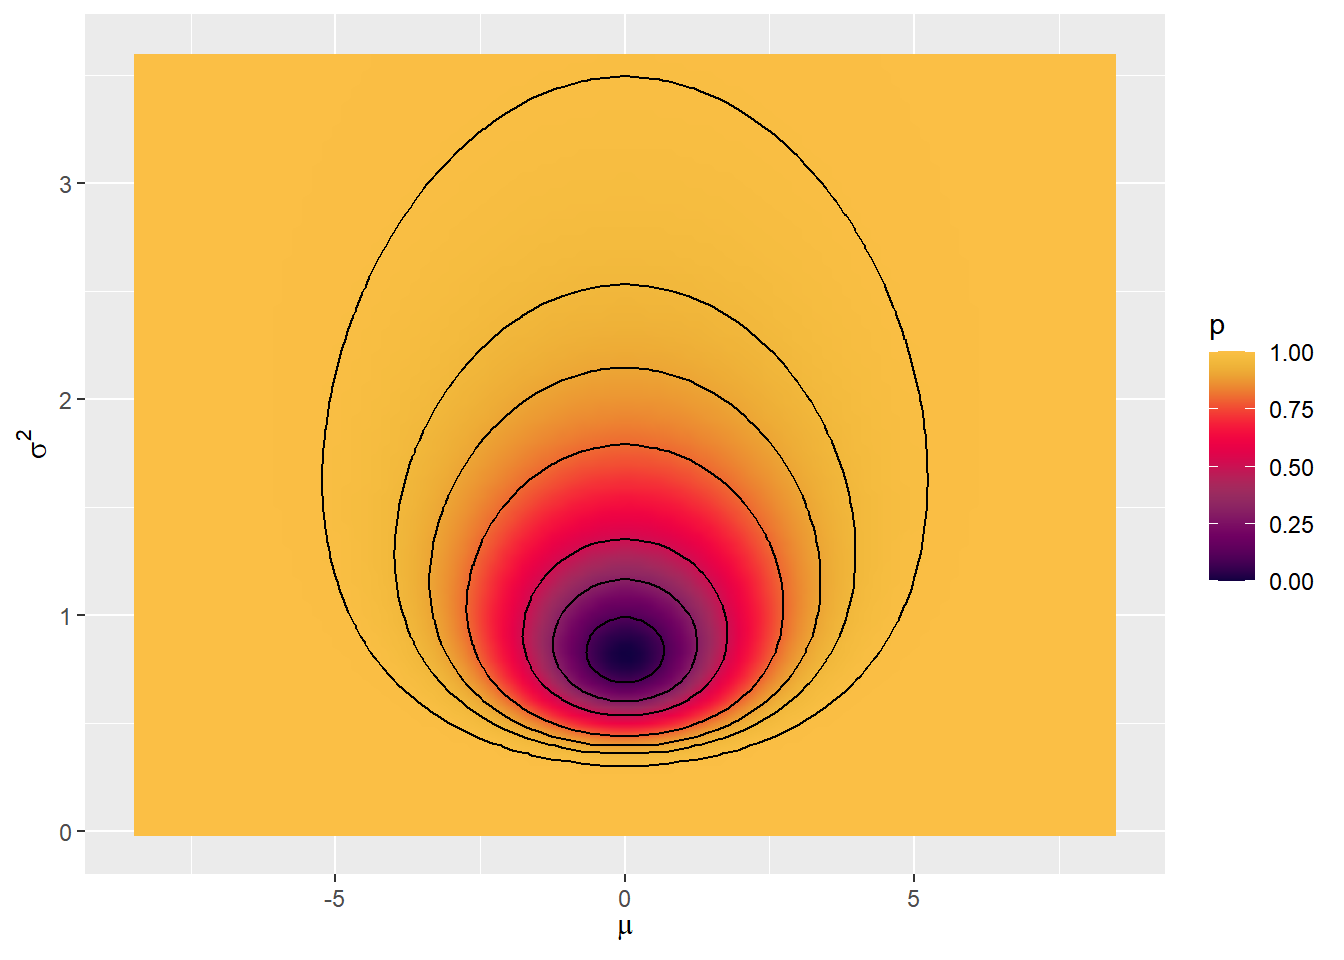
\includegraphics[width=0.8\linewidth]{InfBayes_files/figure-latex/unnamed-chunk-53-1} \end{center}

\(~\)

\hypertarget{monte-carlo-com-amostragem-de-importuxe2ncia}{%
\section{Monte Carlo com Amostragem de Importância}\label{monte-carlo-com-amostragem-de-importuxe2ncia}}

Considere \(f(\theta|\boldsymbol x)\propto f(\boldsymbol x| \theta)f(\theta)\) e suponha que não se sabe simular observações desta distribuição mas tem-se interesse na quantidade \(E\left[g(\theta)|\boldsymbol x\right]=\displaystyle\int_\Theta g(\theta)f(\theta| \boldsymbol x)d\theta\).

Suponha também que existe uma distribuição \(h(\theta)\) que seja uma aproximação para \(f(\theta|\boldsymbol x)\) (preferencialmente com caudas mais pesadas) da qual sabe-se simular. Então,

\(E\left[g(\theta)| \boldsymbol x\right]\)
\(=\displaystyle\int_\Theta g(\theta)f(\theta|\boldsymbol x)d\theta\)
\(=\dfrac{\displaystyle \int_\Theta g(\theta)f(\boldsymbol x|\theta)f(\theta)d\theta}{\displaystyle\int_\theta f(\boldsymbol x|\theta)f(\theta)d\theta}\)
\(=\dfrac{\displaystyle \int g(\theta)\left(\frac{f(\boldsymbol x|\theta)f(\theta)}{h(\theta)}\right)h(\theta)d\theta}{\displaystyle\int\left(\frac{f(\boldsymbol x|\theta)f(\theta)}{h(\theta)}\right)h(\theta)d\theta}\) \(=\dfrac{\displaystyle\int g(\theta)w(\theta)h(\theta)d\theta}{\displaystyle\int w(\theta)h(\theta)d\theta}\)
\(\approx \displaystyle\sum_{i=1}^m \dfrac{w_i}{\sum_{j=1}^mw_j}~g(\theta_i)\),

onde \(w_i=w(\theta_i)=\dfrac{f(\boldsymbol x|\theta_i)f(\theta_i)}{h(\theta_i)}\).

\(~\)

\hypertarget{muxe9todo-de-rejeiuxe7uxe3o}{%
\section{Método de Rejeição}\label{muxe9todo-de-rejeiuxe7uxe3o}}

Considere novamente que o objetivo é simular observações de \(f(\theta|\boldsymbol x)\) mas não é possível fazer isso diretamente. Por outro lado, sabe-se simular dados de uma ``distribuição candidata'', \(h(\theta)\), tal que \(f(\theta|\boldsymbol x)\leq Mh(\theta)\), \(\forall \theta \in \Theta\) e para alguma constante \(M\). A ideia do método é rejeitar pontos gerados em regiões em que \(h\) atribui maior probabilidade que \(f\) com probabilidade \(1-\left[f(\theta|\boldsymbol x)~/~Mh(\theta)\right]\). Para que a afirmação anterior faça sentido, \(M\) deve ser tal que \(f(\theta|\boldsymbol x)~/~ Mh(\theta) \leq 1\), \(\forall \theta \in \Theta\), de modo que a melhor escolha para \(M\) é \(M^*=\underset{\Theta}{\sup}\dfrac{f(\theta|\boldsymbol x)}{h(\theta)}\).

\begin{Shaded}
\begin{Highlighting}[]
\NormalTok{r =}\StringTok{ }\ControlFlowTok{function}\NormalTok{(t)\{}\KeywordTok{dbeta}\NormalTok{(t,}\DecValTok{4}\NormalTok{,}\DecValTok{2}\NormalTok{)}\OperatorTok{/}\KeywordTok{dbeta}\NormalTok{(t,}\DecValTok{1}\NormalTok{,}\DecValTok{1}\NormalTok{)\}}
\NormalTok{M =}\StringTok{ }\KeywordTok{optimize}\NormalTok{(r,}\KeywordTok{c}\NormalTok{(}\DecValTok{0}\NormalTok{,}\DecValTok{1}\NormalTok{),}\DataTypeTok{maximum =} \OtherTok{TRUE}\NormalTok{)}
\KeywordTok{tibble}\NormalTok{(}\DataTypeTok{t =} \KeywordTok{seq}\NormalTok{(}\DecValTok{0}\NormalTok{,}\DecValTok{1}\NormalTok{,}\DataTypeTok{length.out =} \DecValTok{1000}\NormalTok{)) }\OperatorTok\StringTok{ }
\StringTok{  }\KeywordTok{mutate}\NormalTok{(}\DataTypeTok{f=}\KeywordTok{dbeta}\NormalTok{(t,}\DecValTok{4}\NormalTok{,}\DecValTok{2}\NormalTok{), }\DataTypeTok{h=}\KeywordTok{dbeta}\NormalTok{(t,}\DecValTok{1}\NormalTok{,}\DecValTok{1}\NormalTok{),}
         \DataTypeTok{Mh=}\NormalTok{M}\OperatorTok{$}\NormalTok{objective}\OperatorTok{*}\KeywordTok{dbeta}\NormalTok{(t,}\DecValTok{1}\NormalTok{,}\DecValTok{1}\NormalTok{)) }\OperatorTok\StringTok{ }
\StringTok{  }\KeywordTok{ggplot}\NormalTok{() }\OperatorTok{+}\StringTok{ }\KeywordTok{theme_bw}\NormalTok{() }\OperatorTok{+}
\StringTok{  }\KeywordTok{geom_line}\NormalTok{(}\KeywordTok{aes}\NormalTok{(}\DataTypeTok{x=}\NormalTok{t,}\DataTypeTok{y=}\NormalTok{f,}\DataTypeTok{colour=}\StringTok{"'Dist. Interesse' f"}\NormalTok{),}\DataTypeTok{lwd=}\FloatTok{1.1}\NormalTok{) }\OperatorTok{+}
\StringTok{  }\KeywordTok{geom_line}\NormalTok{(}\KeywordTok{aes}\NormalTok{(}\DataTypeTok{x=}\NormalTok{t,}\DataTypeTok{y=}\NormalTok{h,}\DataTypeTok{colour=}\StringTok{"'Dist. Candidata' h"}\NormalTok{),}\DataTypeTok{lwd=}\FloatTok{1.1}\NormalTok{) }\OperatorTok{+}
\StringTok{  }\KeywordTok{geom_line}\NormalTok{(}\KeywordTok{aes}\NormalTok{(}\DataTypeTok{x=}\NormalTok{t,}\DataTypeTok{y=}\NormalTok{Mh,}\DataTypeTok{colour=}\StringTok{"M.h"}\NormalTok{),}\DataTypeTok{lwd=}\FloatTok{1.1}\NormalTok{) }\OperatorTok{+}
\StringTok{  }\KeywordTok{geom_segment}\NormalTok{(}\DataTypeTok{x=}\FloatTok{0.5}\NormalTok{,}\DataTypeTok{xend=}\FloatTok{0.5}\NormalTok{,}\DataTypeTok{y=}\KeywordTok{dbeta}\NormalTok{(}\FloatTok{0.5}\NormalTok{,}\DecValTok{4}\NormalTok{,}\DecValTok{2}\NormalTok{),}\DataTypeTok{yend=}\NormalTok{M}\OperatorTok{$}\NormalTok{objective}\OperatorTok{*}\KeywordTok{dbeta}\NormalTok{(}\FloatTok{0.5}\NormalTok{,}\DecValTok{1}\NormalTok{,}\DecValTok{1}\NormalTok{),}\DataTypeTok{col=}\StringTok{"darkgrey"}\NormalTok{) }\OperatorTok{+}
\StringTok{  }\KeywordTok{geom_segment}\NormalTok{(}\DataTypeTok{x=}\FloatTok{0.5}\NormalTok{,}\DataTypeTok{xend=}\FloatTok{0.5}\NormalTok{,}\DataTypeTok{y=}\DecValTok{0}\NormalTok{,}\DataTypeTok{yend=}\KeywordTok{dbeta}\NormalTok{(}\FloatTok{0.5}\NormalTok{,}\DecValTok{4}\NormalTok{,}\DecValTok{2}\NormalTok{)) }\OperatorTok{+}
\StringTok{  }\KeywordTok{geom_segment}\NormalTok{(}\DataTypeTok{x=}\FloatTok{0.25}\NormalTok{,}\DataTypeTok{xend=}\FloatTok{0.25}\NormalTok{,}\DataTypeTok{y=}\KeywordTok{dbeta}\NormalTok{(}\FloatTok{0.25}\NormalTok{,}\DecValTok{4}\NormalTok{,}\DecValTok{2}\NormalTok{),}\DataTypeTok{yend=}\NormalTok{M}\OperatorTok{$}\NormalTok{objective}\OperatorTok{*}\KeywordTok{dbeta}\NormalTok{(}\FloatTok{0.25}\NormalTok{,}\DecValTok{1}\NormalTok{,}\DecValTok{1}\NormalTok{),}\DataTypeTok{col=}\StringTok{"darkgrey"}\NormalTok{) }\OperatorTok{+}
\StringTok{  }\KeywordTok{geom_segment}\NormalTok{(}\DataTypeTok{x=}\FloatTok{0.25}\NormalTok{,}\DataTypeTok{xend=}\FloatTok{0.25}\NormalTok{,}\DataTypeTok{y=}\DecValTok{0}\NormalTok{,}\DataTypeTok{yend=}\KeywordTok{dbeta}\NormalTok{(}\FloatTok{0.25}\NormalTok{,}\DecValTok{4}\NormalTok{,}\DecValTok{2}\NormalTok{)) }\OperatorTok{+}
\StringTok{  }\KeywordTok{geom_segment}\NormalTok{(}\DataTypeTok{x=}\FloatTok{0.75}\NormalTok{,}\DataTypeTok{xend=}\FloatTok{0.75}\NormalTok{,}\DataTypeTok{y=}\KeywordTok{dbeta}\NormalTok{(}\FloatTok{0.75}\NormalTok{,}\DecValTok{4}\NormalTok{,}\DecValTok{2}\NormalTok{),}\DataTypeTok{yend=}\NormalTok{M}\OperatorTok{$}\NormalTok{objective}\OperatorTok{*}\KeywordTok{dbeta}\NormalTok{(}\FloatTok{0.75}\NormalTok{,}\DecValTok{1}\NormalTok{,}\DecValTok{1}\NormalTok{),}\DataTypeTok{col=}\StringTok{"darkgrey"}\NormalTok{) }\OperatorTok{+}
\StringTok{  }\KeywordTok{geom_segment}\NormalTok{(}\DataTypeTok{x=}\FloatTok{0.75}\NormalTok{,}\DataTypeTok{xend=}\FloatTok{0.75}\NormalTok{,}\DataTypeTok{y=}\DecValTok{0}\NormalTok{,}\DataTypeTok{yend=}\KeywordTok{dbeta}\NormalTok{(}\FloatTok{0.75}\NormalTok{,}\DecValTok{4}\NormalTok{,}\DecValTok{2}\NormalTok{)) }\OperatorTok{+}
\StringTok{  }\KeywordTok{labs}\NormalTok{(}\DataTypeTok{colour=}\StringTok{""}\NormalTok{)}
\end{Highlighting}
\end{Shaded}

\begin{center}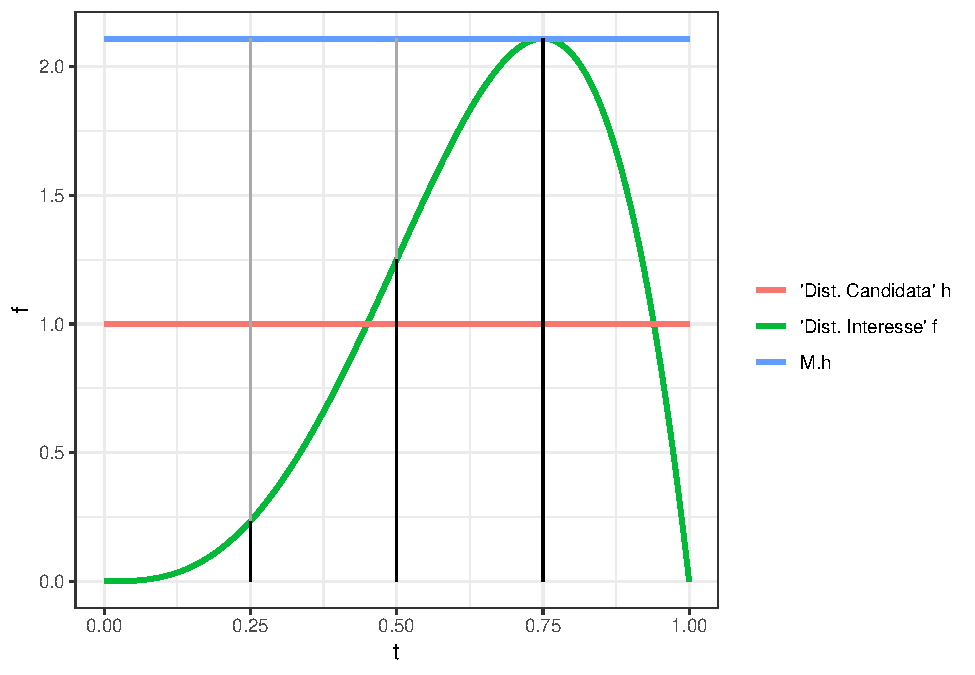
\includegraphics[width=0.8\linewidth]{InfBayes_files/figure-latex/unnamed-chunk-54-1} \end{center}

No exemplo apresentado no gráfico acima, suponha que foram gerados os ``candidatos'' \(0.25\), \(0.5\) e \(0.75\). É possível notar que o ponto \(0.75\) deve ser aceito, o ponto \(0.5\) dever ser aceito com probabilidade \(0.59\) e o ponto \(0.25\) deve ser aceito com probabilidade \(0.11\). A seguir é apresentado o pseudo-algorítmo do método da rejeição.

\begin{quote}
\textbf{Para} \(i=1,...,m\)\\
\(~~~\) \textbf{Repita}\\
\(~~~~~~\) Simule \(u\sim Unif(0,1)\)\\
\(~~~~~~\) Simule \(\theta^\prime\) da distribuição candidata \(h(\theta)\)\\
\(~~~\) \textbf{Até} \(u \leq \frac{f(\theta^\prime|\boldsymbol x)}{Mh(\theta^\prime)}\)\\
\(~~~\) \(\theta_i=\theta^\prime\)\\
\textbf{Fim\_Para}.
\end{quote}

\begin{Shaded}
\begin{Highlighting}[]
\NormalTok{r =}\StringTok{ }\ControlFlowTok{function}\NormalTok{(t)\{(}\FloatTok{0.4}\OperatorTok{*}\KeywordTok{dnorm}\NormalTok{(t,}\OperatorTok{-}\DecValTok{1}\NormalTok{,}\DecValTok{1}\OperatorTok{/}\DecValTok{2}\NormalTok{)}\OperatorTok{+}\FloatTok{0.6}\OperatorTok{*}\KeywordTok{dt}\NormalTok{(t,}\DecValTok{5}\NormalTok{,}\DecValTok{1}\NormalTok{))}\OperatorTok{/}\KeywordTok{dt}\NormalTok{(t,}\DecValTok{1}\NormalTok{)\}}
\NormalTok{M =}\StringTok{ }\KeywordTok{optimize}\NormalTok{(r,}\KeywordTok{c}\NormalTok{(}\OperatorTok{-}\DecValTok{8}\NormalTok{,}\DecValTok{10}\NormalTok{),}\DataTypeTok{maximum =} \OtherTok{TRUE}\NormalTok{)}
\KeywordTok{tibble}\NormalTok{(}\DataTypeTok{t =} \KeywordTok{seq}\NormalTok{(}\OperatorTok{-}\DecValTok{5}\NormalTok{,}\DecValTok{6}\NormalTok{,}\DataTypeTok{length.out =} \DecValTok{1000}\NormalTok{)) }\OperatorTok\StringTok{ }
\StringTok{  }\KeywordTok{mutate}\NormalTok{(}\DataTypeTok{f=}\NormalTok{(}\FloatTok{0.4}\OperatorTok{*}\KeywordTok{dnorm}\NormalTok{(t,}\OperatorTok{-}\DecValTok{1}\NormalTok{,}\DecValTok{1}\OperatorTok{/}\DecValTok{2}\NormalTok{)}\OperatorTok{+}\FloatTok{0.6}\OperatorTok{*}\KeywordTok{dt}\NormalTok{(t,}\DecValTok{5}\NormalTok{,}\DecValTok{1}\NormalTok{)), }\DataTypeTok{h=}\KeywordTok{dt}\NormalTok{(t,}\DecValTok{1}\NormalTok{),}
         \DataTypeTok{Mh=}\NormalTok{M}\OperatorTok{$}\NormalTok{objective}\OperatorTok{*}\KeywordTok{dt}\NormalTok{(t,}\DecValTok{1}\NormalTok{)) }\OperatorTok\StringTok{ }
\StringTok{  }\KeywordTok{ggplot}\NormalTok{() }\OperatorTok{+}\StringTok{ }\KeywordTok{theme_bw}\NormalTok{() }\OperatorTok{+}
\StringTok{  }\KeywordTok{geom_line}\NormalTok{(}\KeywordTok{aes}\NormalTok{(}\DataTypeTok{x=}\NormalTok{t,}\DataTypeTok{y=}\NormalTok{f,}\DataTypeTok{colour=}\StringTok{"'Dist. Interesse' f"}\NormalTok{),}\DataTypeTok{lwd=}\FloatTok{1.1}\NormalTok{) }\OperatorTok{+}
\StringTok{  }\KeywordTok{geom_line}\NormalTok{(}\KeywordTok{aes}\NormalTok{(}\DataTypeTok{x=}\NormalTok{t,}\DataTypeTok{y=}\NormalTok{h,}\DataTypeTok{colour=}\StringTok{"'Dist. Candidata' h"}\NormalTok{),}\DataTypeTok{lwd=}\FloatTok{1.1}\NormalTok{) }\OperatorTok{+}
\StringTok{  }\KeywordTok{geom_line}\NormalTok{(}\KeywordTok{aes}\NormalTok{(}\DataTypeTok{x=}\NormalTok{t,}\DataTypeTok{y=}\NormalTok{Mh,}\DataTypeTok{colour=}\StringTok{"M.h"}\NormalTok{),}\DataTypeTok{lwd=}\FloatTok{1.1}\NormalTok{) }\OperatorTok{+}
\StringTok{  }\KeywordTok{geom_vline}\NormalTok{(}\DataTypeTok{xintercept=}\NormalTok{M}\OperatorTok{$}\NormalTok{maximum,}\DataTypeTok{linetype=}\StringTok{"longdash"}\NormalTok{,}\DataTypeTok{col=}\StringTok{"darkgrey"}\NormalTok{) }\OperatorTok{+}
\StringTok{  }\KeywordTok{labs}\NormalTok{(}\DataTypeTok{colour=}\StringTok{""}\NormalTok{)}
\end{Highlighting}
\end{Shaded}

\begin{center}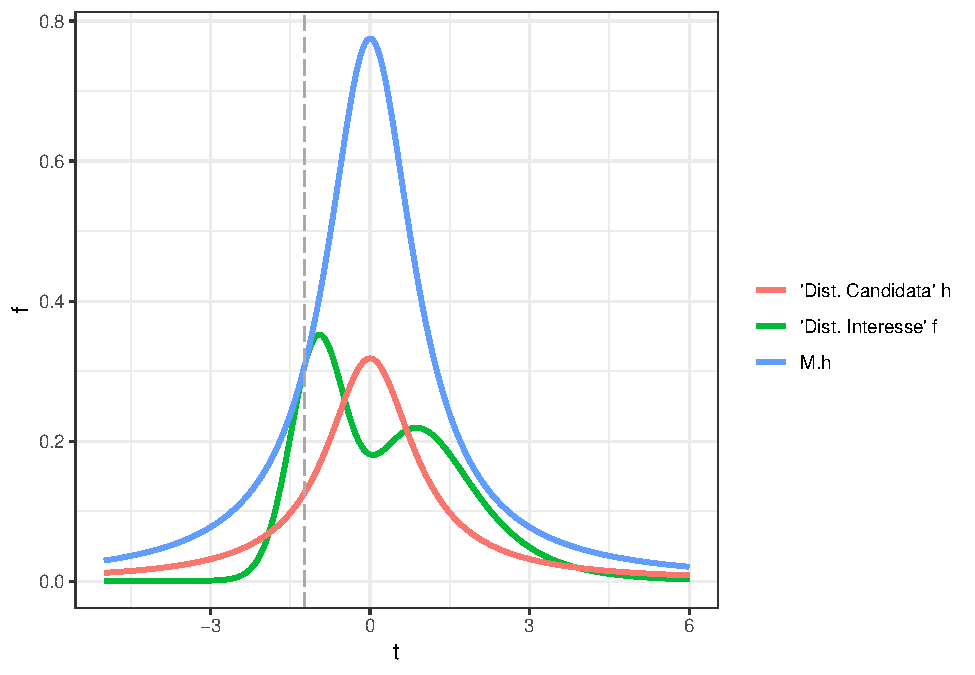
\includegraphics[width=0.8\linewidth]{InfBayes_files/figure-latex/unnamed-chunk-55-1} \end{center}

A linha tracejada representa o ponto na escolha ótima para \(M\). Nesse exemplo é possível notar que na região central, onde é mais ``provável'' gerar observações de \(h\), a razão \(f(\theta|\boldsymbol x)~/~Mh(\theta)\) é menor que \(0.25\), de modo que há uma grande probabilidade de rejeição. Isso justifica a escolha de distribuições candidatas com caudas pesadas. No caso geral, a \emph{probabilidade de aceitação} do método é

\(P\left(\left\{(U,\theta) : U \leq \dfrac{f(\theta|\boldsymbol x)}{Mh(\theta)}\right\}\right)\) \(=E_{U,\theta}\left[\mathbb{I}\left(U \leq \dfrac{f(\theta|\boldsymbol x)}{Mh(\theta)}\right)\right]\) \(=E_{\theta}\left[{E_{U|\theta}\left[\mathbb{I}\left(U \leq \dfrac{f(\theta|\boldsymbol x)}{Mh(\theta)}\right)\right]}\right]\)
\(=E_{\theta}\left[P\left(U \leq \dfrac{f(\theta|\boldsymbol x)}{Mh(\theta)}~\Big|~\theta\right)\right]\)
\(=E_\theta\left[\dfrac{f(\theta|\boldsymbol x)}{Mh(\theta)}\right]\) \(=\displaystyle\int_\Theta\dfrac{f(\theta|\boldsymbol x)}{Mh(\theta)}h(\theta)d\theta\) \(=\dfrac{1}{M}\displaystyle\int_\Theta f(\theta|\boldsymbol x)d\theta=\dfrac{1}{M}\).

\(~\)

No exemplo, a probabilidade de aceitação é \(1/2.434 = 0.41\), ou seja, mais de metade das observações geradas seriam descartadas.

\(~\)

\hypertarget{abc-aproximated-bayesian-computation}{%
\section{ABC (Aproximated Bayesian Computation)}\label{abc-aproximated-bayesian-computation}}

O método ABC é uma forma bastante simples de gerar pontos da distribuição a posteriori. Para sua utilização é suficiente saber gerar pontos da distribuição dos dados e da priori, de modo que a verossimilhança nem precisa ser analiticamente conhecida, fato esse que faz com que o método seja dito ser ``\emph{likelihood-free}''.

Suponha o caso em que \(\boldsymbol X\) é \textbf{discreto} com função de verossimilhança \(f(\boldsymbol x|\theta)\), a priori é \(f(\theta)\) e foi observado \(\boldsymbol X=\boldsymbol x_o\). Abaixo é apresentado o \emph{pseudo-algorítmo} para simular observaçoes da posteriori \(f(\theta |\boldsymbol x_o)\) usando o método ABC.

\begin{quote}
\textbf{Algorítmo ABC (\(\boldsymbol X\) discreto)}\\
\(~\)\\
\textbf{Para} \(i=1,...,m\)\\
\(~~~\) \textbf{Repita}\\
\(~~~~~~\) Gere \(\theta^\prime\) de \(f(\theta)\) (\emph{priori})\\
\(~~~~~~\) Gere \(\boldsymbol y = (y_1,...,y_n)\) de \(f(\boldsymbol x|\theta^\prime)\) (\emph{verossimilhança})\\
\(~~~\) \textbf{Até} \(\boldsymbol y =\boldsymbol x_o\)\\
\(~~~\) \(\theta_i = \theta^\prime\)\\
\textbf{Fim\_Para}
\end{quote}

Para verificar que o método funciona no caso discreto, basta ver que

\(f(\theta_i)\) \(=\displaystyle \sum_{y\in \mathfrak{X}}f(\theta_i)f(\boldsymbol y|\theta_i)\mathbb{I}(\boldsymbol y = \boldsymbol x_o)\)
\(=f(\theta_i)f(\boldsymbol x_o|\theta_i)\)
\(\propto f(\theta |\boldsymbol x_o)\).

\(~\)

No caso em que \(\boldsymbol X\) é contínuo, a probabilidade de gerar uma nova amostra \(\boldsymbol Y\) exatamente igual ao ponto observado \(\boldsymbol x_o\) é zero, \(P(\boldsymbol Y=\boldsymbol x_o)=0\). Nesse caso, o algorítmo é adaptado de modo que são aceitos pontos gerados com \(\Delta\left(\eta(\boldsymbol y),\eta(\boldsymbol x_o)\right) \leq \varepsilon\), onde \(\Delta\) é uma medida de distância conveniente, \(\eta\) é uma estatística (que pode não ser suficiente para \(\theta\)) e \(\varepsilon\) é uma constante de tolerância. O \emph{pseudo-algorítmo} é apresentado a seguir.

\begin{quote}
\textbf{Algorítmo ABC (\(\boldsymbol X\) qualquer)}\\
\(~\)\\
\textbf{Para} \(i=1,...,m\)\\
\(~~~\) \textbf{Repita}\\
\(~~~~~~\) Gere \(\theta^\prime\) de \(f(\theta)\)\\
\(~~~~~~\) Gere \(\boldsymbol y\) de \(f(\boldsymbol x|\theta^\prime)\)\\
\(~~~\) \textbf{Até} \(\Delta(\eta(\boldsymbol x),\eta(\boldsymbol y))\leq \varepsilon\)\\
\(~~~\) \(\theta_i=\theta^\prime\)\\
\textbf{Fim\_Para}
\end{quote}

\(~\)

\(~\)

\hypertarget{mcmc---monte-carlo-via-cadeias-de-markov}{%
\section{MCMC - Monte Carlo via Cadeias de Markov}\label{mcmc---monte-carlo-via-cadeias-de-markov}}

\hypertarget{pequena-introduuxe7uxe3o-uxe0s-cadeias-de-markov}{%
\subsection{Pequena Introdução às Cadeias de Markov}\label{pequena-introduuxe7uxe3o-uxe0s-cadeias-de-markov}}

\textbf{Definição} Um \emph{processo estocástico} (em tempo discreto) é uma sequência de v.a. \(X_0,X_1,X_2,...\) indexada em \(\mathbb{N}\) (os indices podem indicar, por exemplo, tempo ou espaço ou ?). O conjunto \(E\) onde \(X_i\) toma valores é chamado de \emph{espaço de estados}.

\(~\)

\textbf{Definição} Um processo estocásticos é dito uma \emph{Cadeia de Markov} (em tempo discreto) se, \(\forall n \geq 1\) e \(\forall A \subseteq E\),

\(P(X_{n+1}\in A|X_{n}=x_{n},...,X_1=x_1,X_0=x_0)\) \(=P(X_{n+1}\in A|X_{n}=x_{n})\)

\(~\)

\begin{quote}
\textbf{Exemplo 1.} Suponha uma sequência de v.a. \(\left(X_n\right)_{n\geq 1}\) i.i.d. tais que \(p=P(X_1=1)=1-P(X_1=-1)\). Defina \(S_n=\displaystyle \sum_{i=1}^n X_i\) e \(X_0=c\). O processo estocástico \((S_n)_{n\geq 0}\) é uma Cadeia de Markov. De fato,\\
\(P\left(S_n=s_n|S_{n-1}=s_{n-1},\ldots,S_0=s_0\right)\)
\(=\displaystyle P\left(X_n+S_{n-1}=s_{n}|S_{n-1}=s_{n-1},\ldots,S_0=s_0\right)\)\\
\(=\displaystyle P\left(X_n=s_n-s_{n-1}|S_{n-1}=s_{n-1},\ldots,S_0=s_0\right)\)
\(=\displaystyle P\left(X_n=s_n-s_{n-1}|S_{n-1}=s_{n-1}\right)\)
\(=\displaystyle P\left(S_n=s_n|S_{n-1}=s_{n-1}\right)\)
\end{quote}

\begin{center}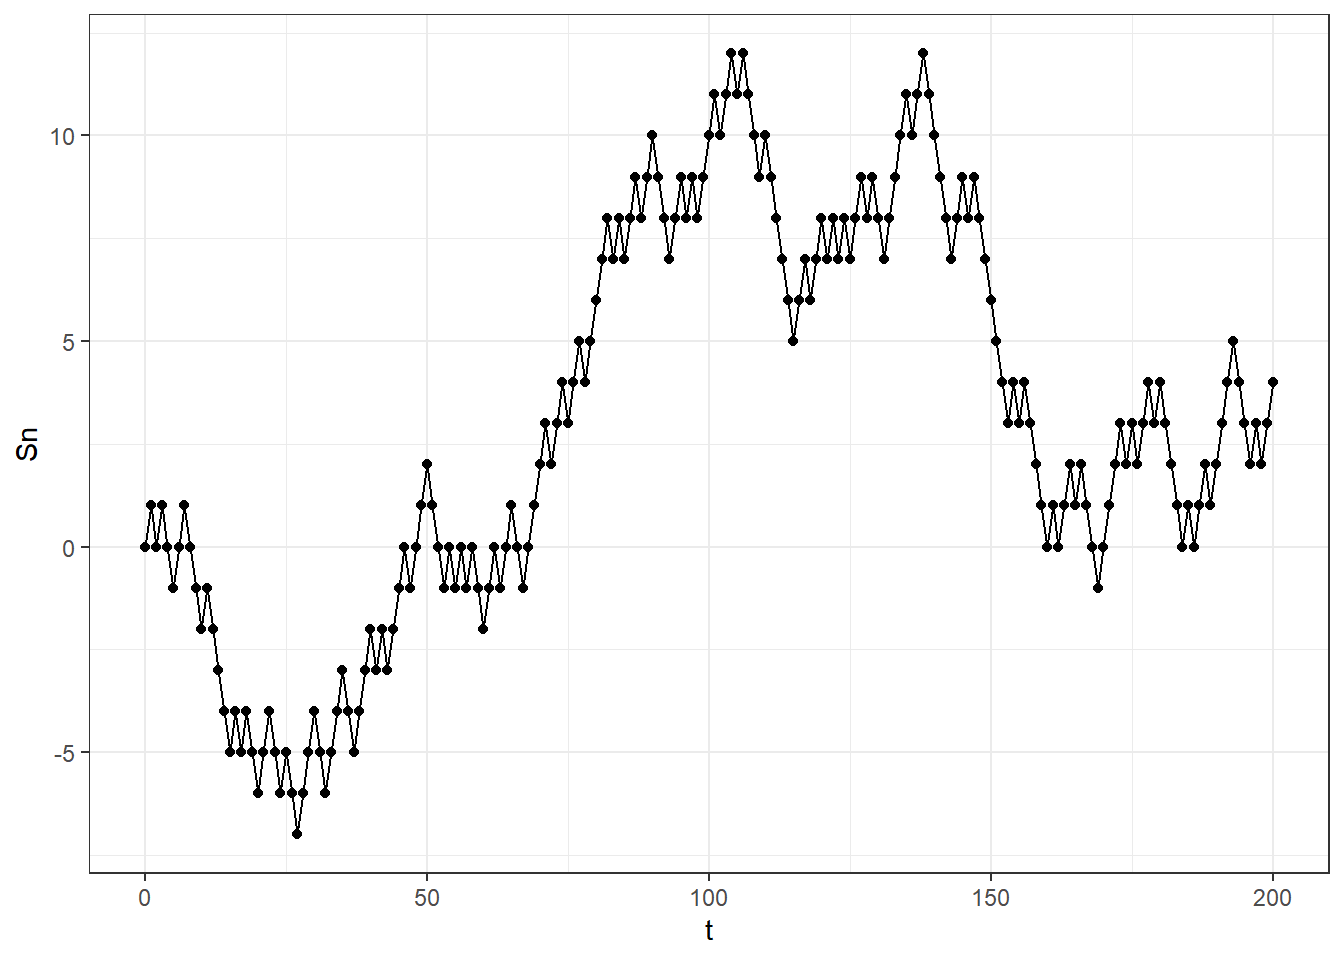
\includegraphics[width=0.8\linewidth]{InfBayes_files/figure-latex/unnamed-chunk-56-1} \end{center}

\(~\)

Uma Cadeia de Markov é caracterizada pela distribuição do \emph{estado inicial} \(X_0\) e pelas \emph{probabilidades de transição} \(Q(x,A)=P(X_n\in A|X_{n-1}=x)\). Se \(Q(x,A)\) não depende de \(n\), dizemos que é \emph{homogênea no tempo}.

\(~\)

Para cada \(n\), a cadeia pode

\begin{enumerate}
\def\labelenumi{\arabic{enumi}.}
\item
  Continuar no estado anterior \(x\), ou seja, \(X_{n+1}=x,\) com probabilidade \(r(x),~ 0\leq r<1\), ou
\item
  Saltar para um estado \(y\) segundo uma função de densidade de probabilidade \(q(x,y)\), onde \(0<\displaystyle\int_E q(x,y)dy=1-r(x)\leq 1\) (sub-probabilidade). No caso discreto vamos considerar \(q(x,x)=0\).
\end{enumerate}

Assim, \(Q(x,A)\) \(=P(X_{n+1}\in A|X_{n}=x)\) \(=\displaystyle\int_A q(x,y)dy+r(x)\mathbb{I}_A(x)\).

\(~\)

Suponha que para um dado \(n\), \(X_n\) tem densidade \(\lambda\), isto é, \(P(X_n\in A)=\displaystyle\int_A\lambda(x)dx\). Então, a densidade de \(X_{n+1}\) pode ser obtida por

\(P(X_{n+1}\in A)~\overset{\begin{array}{c} \text{regra da }\\ \text{prob. total}\end{array}}{=}~ \displaystyle\int_E \lambda(x)~Q(x,A)dx\) \(=\displaystyle\int_E\lambda(x)\left[\int_A q(x,y)dy+r(x)\mathbb{I}_A(x)\right]dx\) \(=\displaystyle\int_A\int_E\lambda(x)q(x,y)dxdy+\int_E\lambda(x)r(x)\mathbb{I}_A(x)dx\) \(=\displaystyle\int_A\int_E\lambda(x)q(x,y)dxdy+\int_A\lambda(y)r(y)dy\)
\(=\displaystyle \int_A\underbrace{\left[\int_E\lambda(x)q(x,y)dx+\lambda(y)r(y)\right]}_{\text{f.d.p. de }X_{n+1}}dy\).

Assim, a f.d.p de \(X_{n+1}\) é \(\lambda Q(y)= \displaystyle\int_E\lambda(x)q(x,y)dx+\lambda(y)r(y)\)

\(~\)

Dizemos que a densidade \(\pi\) é \emph{invariante} (\emph{estacionária}) se as densidades de \(X_{n}\) e \(X_{n+1}\) são iguais (q.c), isto é, \(\pi=\pi Q\) ou \(\int_A \pi(x)dx=\int_E \pi(x)Q(x,A)dx\).

\(~\)

\textbf{Resultado 1.} A afirmação anterior é equivalente a \(\int\pi(x)q(x,y)dx=(1-r(x))\pi(y)\).

\(~\)

\textbf{Resultado 2.} Se a função \(q(x,y)\) satisfaz a condição de \emph{reversibilidade}, isto é, \(\pi(x)q(x,y)=\pi(y)q(y,x)\), então \(\pi\) é uma \emph{medida invariante} da cadeia com função de transição \(Q(x,\cdot)\).

\(~\)

\begin{quote}
\textbf{Demo 1.}\\
\(\displaystyle\int_E\pi(x)q(x,y)dx\)
\(=\displaystyle\int_E\pi(y)q(y,x)dx\) \(=\displaystyle\pi(y)\underbrace{\int_Eq(y,x)dx}_{1-r(y)}\)
\end{quote}

\(~\)

\begin{quote}
\textbf{Demo 2.}\\
\(\displaystyle\int_E \pi(x)Q(x,A)dx\)
\(=\displaystyle\int_E\pi(x)\left[\int_Aq(x,y)dy\right]dx+\int_E \pi(x) r(x)\mathbb{I}_A(x)dx\) \(=\displaystyle\int_A\left[\int_E\pi(x)q(x,y)dx\right]dy+\int_A\pi(x)r(x)dx\)
\(=\displaystyle\int_A\left[\int_E\pi(y)q(y,x)dx\right]dy+\int_A\pi(y)r(y)dx\)
\(=\displaystyle\int_A\pi(y)\left[\int_Eq(y,x)dx\right]dy+\int_A\pi(y)r(y)dy\)
\(=\displaystyle\int_A\pi(y)\Big[1-r(y)\Big]dy+\int_A\pi(y)r(y)dy\)
\(=\displaystyle\int_A\pi(y)\Big[1-r(y)+r(y)\Big]dy\)
\(=\displaystyle\int_A\pi(y)dy\).
\end{quote}

\(~\)

\hypertarget{o-algoritmo-de-metruxf3polis-hastings}{%
\subsection{\texorpdfstring{O algoritmo de \textbf{Metrópolis-Hastings}}{O algoritmo de Metrópolis-Hastings}}\label{o-algoritmo-de-metruxf3polis-hastings}}

Suponha que deseja-se gerar observações de \(\pi(\theta)\propto f(\boldsymbol x|\theta)f(\theta)\propto f(\theta|\boldsymbol x)\). Defina uma Cadeia de Markov \((Y_n)_{n\geq 1}\) tal que, no instante \(n\), \(Y_n=y\). No instante \(n+1\), um candidato \(z\) é gerado segundo a densidade \(q(y,z)\) e é aceito com probabilidade \(\alpha(y,z)\). Isto é, se \(Y_n=y\),

\(Y_{n+1}=\left\{\begin{array}{rcl} z,& \text{com probabilidade}& \alpha(y,z)\\ y,& \text{com probabilidade}& 1-\alpha(y,z)\end{array}\right.\),

em que \(\alpha\) é dado por

\(\alpha(y,z)=\left\{\begin{array}{cl} min\left\{ \dfrac{\pi(z)q(z,y)}{\pi(y)q(y,z)}~,~1\right\},& \text{ se }~ \pi(y)q(y,z)>0\\ 1,& \text{c.c.}\end{array}\right.\)

\(~\)

\textbf{Resultado:} O algoritmo de M-H gera uma cadeia reversível com respeito a \(\pi\) e, portanto, tem \(\pi\) como distribuição estacionária.

\(~\)

\begin{quote}
\textbf{Demo.} Deve-se mostrar que \(\pi(y)\underbrace{q(y,z)\alpha(y,z)}_{p(y,z)}=\pi(z)\underbrace{q(z,y)\alpha(z,y)}_{p(z,y)}~.\)\\
Suponha \(\pi(z)q(z,y)\geq \pi(y)q(y,z)\) (o caso \(~\leq~\) é análogo)\\
i) Se \(\pi(z)q(z,y)=0\Rightarrow\pi(y)q(y,z)=0\) e vale a reversibilidade.\\
ii) \(\pi(z)q(z,y)>0 ~\Rightarrow~ \alpha(y,z)=1\) e \(\alpha(z,y)=\dfrac{\pi(y)q(y,z)}{\pi(z)q(z,y)}\).\\
Nesse caso, \(\pi(z)q(z,y)\alpha(z,y)=\) \(\pi(z)q(z,y)\dfrac{\pi(y)q(y,z)}{\pi(z)q(z,y)}\) \(=\pi(y)q(y,z)\) \(=\pi(y)q(y,z)\alpha(y,z)\)
\end{quote}

\(~\)

\(~\)

\hypertarget{amostrador-de-gibbs}{%
\subsection{Amostrador de Gibbs}\label{amostrador-de-gibbs}}

Suponha que a \(dim(\Theta)>1\) e deseja-se amostrar \(f(\boldsymbol \theta| \boldsymbol x)\) e suponha que é possível obter amostras das distribuições \emph{condicionais completas}, isto é, de \(f(\theta_i| \boldsymbol \theta_{-i},\boldsymbol x)\), onde \(\boldsymbol \theta_{-i}=(\theta_1,...,\theta_{i-1},\theta_{i+1},\theta_k)\). Note que \(f(\theta_i| \boldsymbol \theta_{-i},\boldsymbol x)\propto f(\boldsymbol \theta| \boldsymbol x)=f(\boldsymbol x|\boldsymbol \theta)f(\boldsymbol \theta)\). O método do \emph{Amostrador de Gibbs} é um caso particular do algorítmo de Metrópolis-Hastings em que é gerada uma cadeia \(\left(\boldsymbol \theta^{(n)}\right)_{n\geq 1}\) com \(\alpha(\boldsymbol{y},\boldsymbol{z})=1\) e \(q(\boldsymbol{y},z)=f\left({\theta}_j=\boldsymbol{z}~ \big|~ \boldsymbol{\theta}_{-j}=\boldsymbol{y},~\boldsymbol{x}\right)\), gerada segundo o algorítmo a seguir.

\begin{quote}
\textbf{Algorítmo - Amostrador de Gibbs}\\
\(~\)\\
\(~~~\) Defina uma ``chute inicial'' \(\boldsymbol \theta^{(0)}\) (por exemplo, gerado da priori \(f(\boldsymbol \theta)\) ou fixado)
\textbf{Para} \(i=1,...,m\)\\
\(~~~\) Gere \(\theta_1^{(i)}\) de \(f(\theta_1| \boldsymbol \theta_{-1}^{(i-1)},\boldsymbol x)\)\\
\(~~~\) Gere \(\theta_2^{(i)}\) de \(f(\theta_2| \theta_{1}^{(i)}, \theta_{3}^{(i-1)},\ldots, \theta_{k}^{(i-1)} ,\boldsymbol x)\)\\
\(~~~\) \(~~~\vdots\)\\
\(~~~\) Gere \(\theta_{k-1}^{(i)}\) de \(f(\theta_{k-1}| \theta_{1}^{(i)},\ldots, \theta_{k-2}^{(i)}, \theta_{k}^{(i-1)} ,\boldsymbol x)\)\\
\(~~~\) Gere \(\theta_k^{(i)}\) de \(f(\theta_k| \boldsymbol \theta_{-k}^{(i)} ,\boldsymbol x)\)\\
\textbf{Fim\_Para}
\end{quote}

\(~\)

Os métodos de Metropolis-Hastings descritos anteriormente geram observações de cadeias de Markov com distribuição estacionária que coincide com a posteriori. Contudo, deve-se tomar dois cuidados para a utilização de métodos de Monte Carlo usando essas observalções. O primeiro é que é necessário verificar se a cadeia já atingiu a estacionariedade. Essa verificação é feita, em geral, observando os gráficos das cadeias geradas e, em geral, as primeiras \(b\) observações são descartadas (\emph{burn-in}). Outra possibilidade para verificar a estacionariedade da cadeia, bem como a influência do chute inicial, é gerar duas ou mais cadeias iniciando-se de pontos distintos. Outro problema é a dependência entre as observações geradas. Para contornar esse problema, normalmente uma distância \(k\) entre as observações que serão consideradas na amostra final (\emph{thin}) e as observações entre estas são descartadas. Assim, a amostra final é formada pelos pontos \(\boldsymbol \theta_b, \boldsymbol \theta_{b+k}, \boldsymbol \theta_{b+2k},\ldots,\boldsymbol \theta_{M}\).

\(~\)

\begin{quote}
\textbf{Exemplo 1.} Seja \(X_1,\ldots,X_n\) c.i.i.d. tais que \(X_i~|~\theta_1,\theta_2 \sim \textit{Exp}\left(\theta_1\theta_2\right)\) e considere que a priori \(\theta_i \sim \textit{Gama}\left(a_1,b_i\right)\), \(i=1,2\). Assim,\\
\(f(\boldsymbol \theta|\boldsymbol x)\)
\(\propto f(\boldsymbol x|\boldsymbol \theta) f(\theta_1)f(\theta_2)\)
\(\propto (\theta_1 \theta_2)^n~e^{-\theta_1\theta_2\sum x_i}~~\theta_1^{a_1-1}e^{-b_1\theta_1}~~\theta_2^{a_2-1}e^{-b_2\theta_2}\)
\(\propto \theta_1^{a_1+n-1}~\theta_2^{a_2+n-1}~~e^{-b_1\theta_1-b_2\theta_2 -\theta_1\theta_2\sum x_i}~.\)\\
Essa distribuição não é conhecida mas é possível obter as distribuições condicionais completas\\
\(f(\theta_i|\theta_j,\boldsymbol x) \propto \theta_i^{a_i+n-1}~e^{-\left[b_i \theta_j\sum x_i\right]\theta_i}\) \(\Longrightarrow \theta_i~|~\theta_j,\boldsymbol x \sim \textit{Gama}\left(a_i+n,b_i+\theta_j\sum x_i\right)\),\\
e, portanto, é possível simular observações da posteriori usando o amostrador de Gibbs.
\end{quote}

\begin{Shaded}
\begin{Highlighting}[]
\KeywordTok{set.seed}\NormalTok{(}\DecValTok{666}\NormalTok{)}
\NormalTok{a1=}\DecValTok{2}\NormalTok{; b1=}\DecValTok{3}
\NormalTok{a2=}\DecValTok{3}\NormalTok{; b2=}\DecValTok{2}
\NormalTok{n=}\DecValTok{8}
\NormalTok{sumx=}\DecValTok{4}
\NormalTok{M=}\DecValTok{10000}
\NormalTok{theta1=}\KeywordTok{vector}\NormalTok{(}\DataTypeTok{length =}\NormalTok{ M)}
\NormalTok{theta2=}\KeywordTok{vector}\NormalTok{(}\DataTypeTok{length =}\NormalTok{ M)}
\NormalTok{theta1[}\DecValTok{1}\NormalTok{] =}\StringTok{ }\DecValTok{4}
\NormalTok{theta2[}\DecValTok{1}\NormalTok{] =}\StringTok{ }\DecValTok{4}
\ControlFlowTok{for}\NormalTok{(i }\ControlFlowTok{in} \DecValTok{2}\OperatorTok{:}\NormalTok{M)\{}
\NormalTok{  theta1[i] =}\StringTok{ }\KeywordTok{rgamma}\NormalTok{(}\DecValTok{1}\NormalTok{,a1}\OperatorTok{+}\NormalTok{n,b1}\OperatorTok{+}\NormalTok{theta2[i}\DecValTok{-1}\NormalTok{]}\OperatorTok{*}\NormalTok{sumx)}
\NormalTok{  theta2[i] =}\StringTok{ }\KeywordTok{rgamma}\NormalTok{(}\DecValTok{1}\NormalTok{,a2}\OperatorTok{+}\NormalTok{n,b2}\OperatorTok{+}\NormalTok{theta1[i]}\OperatorTok{*}\NormalTok{sumx)}
\NormalTok{\}}
\NormalTok{m=}\DecValTok{200}\NormalTok{; sel=}\KeywordTok{seq}\NormalTok{(}\DecValTok{1}\NormalTok{,m)}
\KeywordTok{tibble}\NormalTok{(}\DataTypeTok{theta1=}\NormalTok{theta1[sel],}\DataTypeTok{theta2=}\NormalTok{theta2[sel],}\DataTypeTok{t=}\KeywordTok{seq}\NormalTok{(}\DecValTok{1}\NormalTok{,}\KeywordTok{length}\NormalTok{(sel))) }\OperatorTok
\StringTok{  }\KeywordTok{ggplot}\NormalTok{() }\OperatorTok{+}\StringTok{ }\KeywordTok{theme_bw}\NormalTok{() }\OperatorTok{+}
\StringTok{  }\KeywordTok{geom_path}\NormalTok{(}\KeywordTok{aes}\NormalTok{(theta1,theta2),}\DataTypeTok{col=}\StringTok{"darkgrey"}\NormalTok{) }\OperatorTok{+}
\StringTok{  }\KeywordTok{geom_point}\NormalTok{(}\KeywordTok{aes}\NormalTok{(theta1,theta2)) }\OperatorTok{+}
\StringTok{  }\KeywordTok{xlab}\NormalTok{(}\KeywordTok{expression}\NormalTok{(theta[}\DecValTok{1}\NormalTok{])) }\OperatorTok{+}\StringTok{ }\KeywordTok{ylab}\NormalTok{(}\KeywordTok{expression}\NormalTok{(theta[}\DecValTok{2}\NormalTok{]))}
\end{Highlighting}
\end{Shaded}

\begin{center}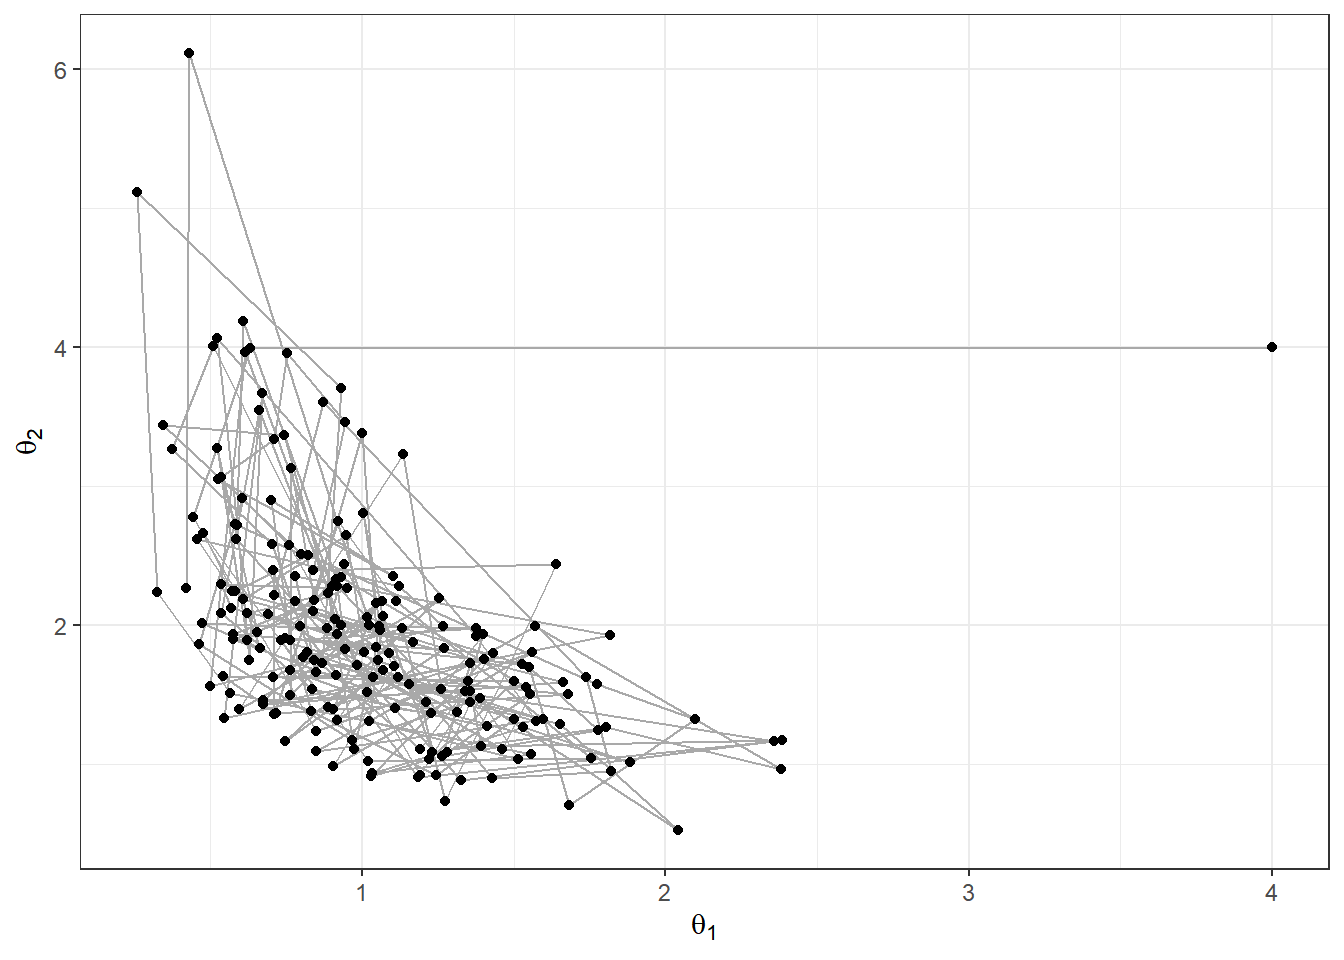
\includegraphics[width=0.8\linewidth]{InfBayes_files/figure-latex/unnamed-chunk-57-1} \end{center}

A seguir, são apresentados os gráficos das cadeias geradas e das autocorrelações.

\begin{center}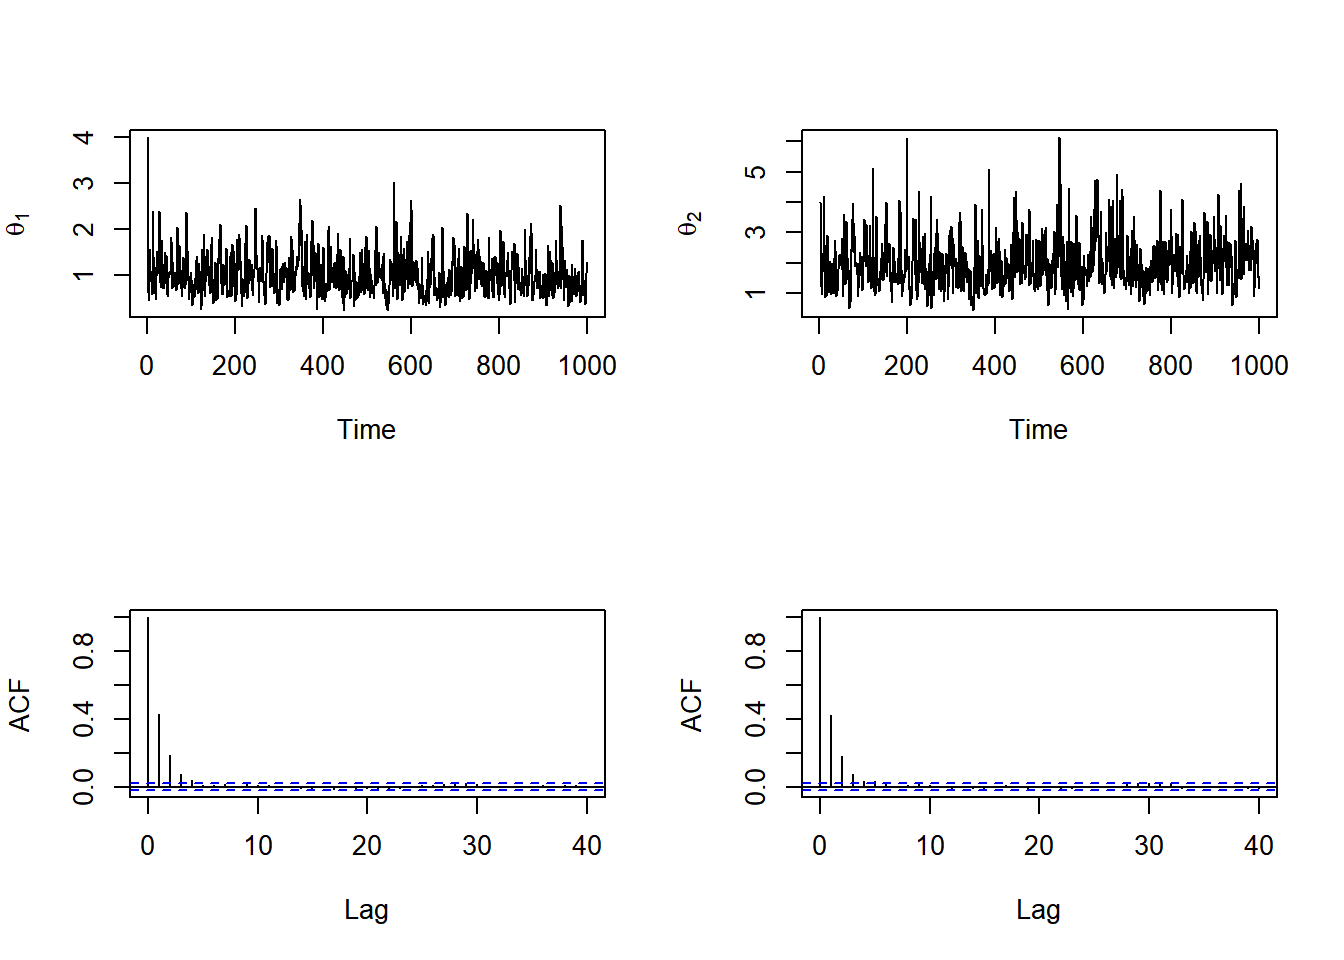
\includegraphics[width=0.8\linewidth]{InfBayes_files/figure-latex/unnamed-chunk-59-1} \end{center}

Aparentemente, a cadeia converge rapidamente para a distribuição estacionária mas as autocorrelações entre observações consecutivas é alta. Assim, vamos descartar as 10 primeiras observações e considerar saltos de tamanho 5. Os novo gráficos são apresentados abaixo.

\begin{center}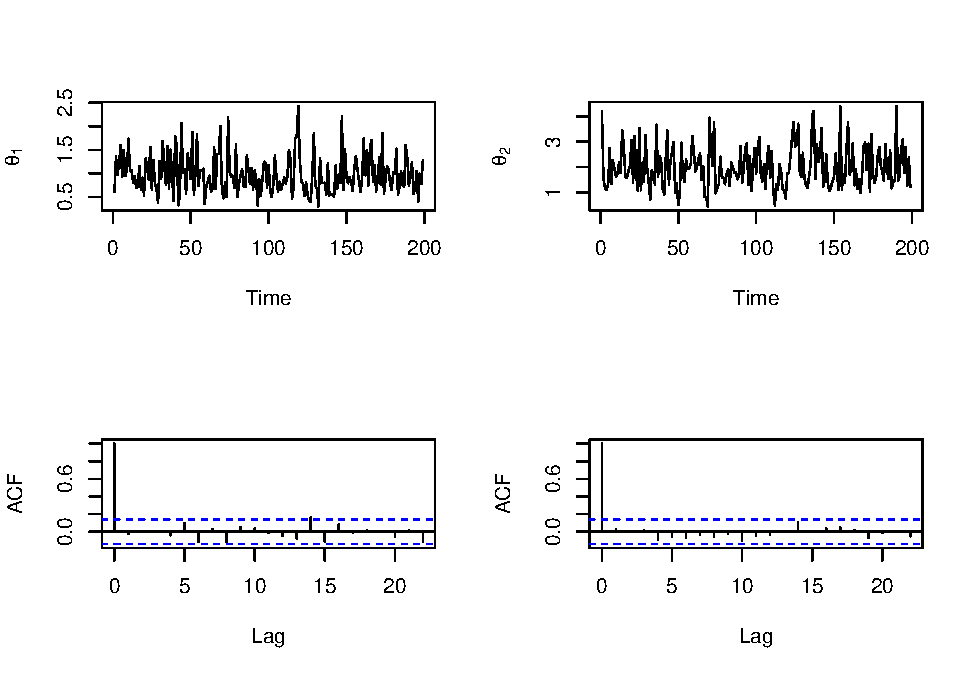
\includegraphics[width=0.8\linewidth]{InfBayes_files/figure-latex/unnamed-chunk-60-1} \end{center}

Por fim são apresentadas as estimativas das densidades marginais e as regiões HPD.

\begin{center}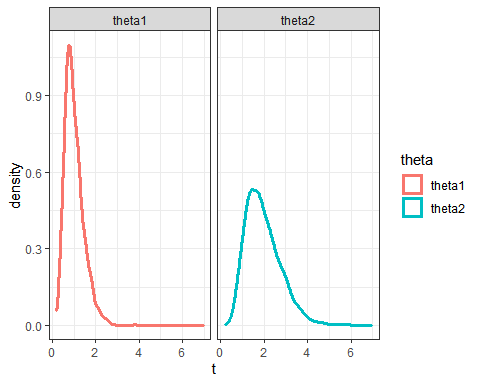
\includegraphics[width=0.8\linewidth]{InfBayes_files/figure-latex/unnamed-chunk-61-1} \end{center}

\begin{Shaded}
\begin{Highlighting}[]
\NormalTok{sel=}\KeywordTok{seq}\NormalTok{(}\DecValTok{10}\NormalTok{,M,}\DecValTok{5}\NormalTok{)}
\NormalTok{dpost=}\KeywordTok{Vectorize}\NormalTok{(}\ControlFlowTok{function}\NormalTok{(t1,t2)\{ }\CommentTok{#densidade posterior}
  \KeywordTok{exp}\NormalTok{((n}\DecValTok{-1}\NormalTok{)}\OperatorTok{*}\KeywordTok{log}\NormalTok{(t1}\OperatorTok{*}\NormalTok{t2)}\OperatorTok{+}\KeywordTok{dexp}\NormalTok{(sumx,t1}\OperatorTok{*}\NormalTok{t2,}\DataTypeTok{log=}\OtherTok{TRUE}\NormalTok{)}\OperatorTok{+}\KeywordTok{dgamma}\NormalTok{(t1,a1,b1,}\DataTypeTok{log=}\OtherTok{TRUE}\NormalTok{)}\OperatorTok{+}\KeywordTok{dgamma}\NormalTok{(t2,a2,b2,}\DataTypeTok{log=}\OtherTok{TRUE}\NormalTok{))\})}
\CommentTok{# simulações}
\NormalTok{df =}\StringTok{ }\KeywordTok{tibble}\NormalTok{(}\DataTypeTok{theta1=}\NormalTok{theta1[sel],}\DataTypeTok{theta2=}\NormalTok{theta2[sel]) }\OperatorTok\StringTok{ }
\StringTok{      }\KeywordTok{mutate}\NormalTok{(}\DataTypeTok{post=}\KeywordTok{dpost}\NormalTok{(theta2,theta2))}
\CommentTok{# variáveis para os gráficos}
\NormalTok{gama=}\KeywordTok{c}\NormalTok{(}\FloatTok{0.99}\NormalTok{,}\FloatTok{0.95}\NormalTok{,}\FloatTok{0.9}\NormalTok{,}\FloatTok{0.8}\NormalTok{,}\FloatTok{0.5}\NormalTok{,}\FloatTok{0.3}\NormalTok{,}\FloatTok{0.1}\NormalTok{) }\CommentTok{# prob das regiões}
\NormalTok{l=}\KeywordTok{quantile}\NormalTok{(df}\OperatorTok{$}\NormalTok{post,}\DecValTok{1}\OperatorTok{-}\NormalTok{gama)}
\NormalTok{d=}\DecValTok{1000}
\NormalTok{x=}\KeywordTok{seq}\NormalTok{(}\DecValTok{0}\NormalTok{,}\DecValTok{12}\NormalTok{,}\DataTypeTok{length.out =}\NormalTok{ d)}
\NormalTok{y=}\KeywordTok{seq}\NormalTok{(}\DecValTok{0}\NormalTok{,}\DecValTok{12}\NormalTok{,}\DataTypeTok{length.out =}\NormalTok{ d)}
\NormalTok{z=}\KeywordTok{apply}\NormalTok{(}\KeywordTok{cbind}\NormalTok{(}\KeywordTok{rep}\NormalTok{(x,d),}\KeywordTok{rep}\NormalTok{(y,}\DataTypeTok{each=}\NormalTok{d)),}\DecValTok{1}\NormalTok{,}\ControlFlowTok{function}\NormalTok{(t)\{}\KeywordTok{dpost}\NormalTok{(t[}\DecValTok{1}\NormalTok{],t[}\DecValTok{2}\NormalTok{])\})}
\CommentTok{# gráfico das regiões HPD de prob. gama=c(0.99,0.95,0.9,0.8,0.5,0.3,0.1)}
\KeywordTok{tibble}\NormalTok{(}\DataTypeTok{x1=}\KeywordTok{rep}\NormalTok{(x,d),}\DataTypeTok{y1=}\KeywordTok{rep}\NormalTok{(y,}\DataTypeTok{each=}\NormalTok{d),}\DataTypeTok{z1=}\NormalTok{z) }\OperatorTok
\StringTok{  }\KeywordTok{arrange}\NormalTok{(z1) }\OperatorTok\StringTok{ }\KeywordTok{mutate}\NormalTok{(}\DataTypeTok{p=}\DecValTok{1}\OperatorTok{-}\NormalTok{(}\KeywordTok{cumsum}\NormalTok{(z1)}\OperatorTok{/}\KeywordTok{sum}\NormalTok{(z1))) }\OperatorTok
\StringTok{  }\KeywordTok{ggplot}\NormalTok{(}\KeywordTok{aes}\NormalTok{(x1,y1,}\DataTypeTok{z=}\NormalTok{z1,}\DataTypeTok{fill =}\NormalTok{ p)) }\OperatorTok{+}
\StringTok{  }\KeywordTok{geom_raster}\NormalTok{(}\DataTypeTok{interpolate =} \OtherTok{TRUE}\NormalTok{) }\OperatorTok{+}
\StringTok{  }\NormalTok{jcolors}\OperatorTok{::}\KeywordTok{scale_fill_jcolors_contin}\NormalTok{(}\StringTok{"pal3"}\NormalTok{) }\OperatorTok{+}
\StringTok{  }\KeywordTok{geom_contour}\NormalTok{(}\DataTypeTok{breaks=}\NormalTok{l,}\DataTypeTok{col=}\StringTok{"black"}\NormalTok{) }\OperatorTok{+}
\StringTok{  }\KeywordTok{xlab}\NormalTok{(}\KeywordTok{expression}\NormalTok{(theta[}\DecValTok{1}\NormalTok{])) }\OperatorTok{+}\StringTok{ }\KeywordTok{ylab}\NormalTok{(}\KeywordTok{expression}\NormalTok{(theta[}\DecValTok{2}\NormalTok{]))}
\end{Highlighting}
\end{Shaded}

\begin{center}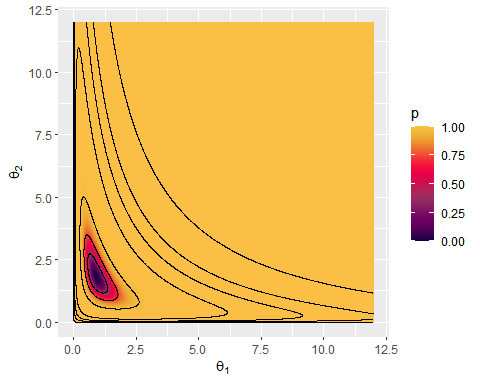
\includegraphics[width=0.8\linewidth]{InfBayes_files/figure-latex/unnamed-chunk-62-1} \end{center}

\hypertarget{bibliotecas-de-r-para-inferuxeancia-bayesiana}{%
\section{Bibliotecas de R para Inferência Bayesiana}\label{bibliotecas-de-r-para-inferuxeancia-bayesiana}}

Nessa seção serão apresentadas algumas bibliotecas do R para inferência Bayesiana, em especial, \texttt{LaplacesDemon} e \texttt{Stan}, que são bibliotecas utilizadas para simular dados da posteriori. Para isso, será apresentado como exemplo o modelo de regressão linear, possivelmente um dos métodos mais usados nas aplicações de inferência estatística.

\hypertarget{o-modelo-de-regressuxe3o-linear}{%
\subsection{O Modelo de Regressão Linear}\label{o-modelo-de-regressuxe3o-linear}}

Considere \(n\) observações de uma variável aleatória de interesse (chamada de \emph{variável dependente} ou \emph{variável resposta}) e de \(p-1\) características associadas a cada uma dessas observações (chamadas de \emph{variáveis dependentes} ou \emph{explicativas} ou \emph{covariáveis}), supostamente fixadas. Um modelo de regressão linear pode ser escrito como

\[\boldsymbol{Y} = \boldsymbol{X}\boldsymbol{\beta} + \boldsymbol{\epsilon}\]
com
\(~\boldsymbol{Y} = \left[\begin{array}{c} Y_1\\ Y_2\\ \vdots\\ Y_n \end{array}\right]~~\);
\(~~~\boldsymbol{X} = \left[\begin{array}{cccc} 1 & x_{11} & \cdots & x_{1,p-1}\\ 1 & x_{21} & \cdots & x_{2,p-1}\\ \vdots & \vdots & \ddots & \vdots \\ 1 & x_{n1} & \cdots & x_{n,p-1} \end{array}\right]~~\);
\(~~~\boldsymbol{\beta} = \left[\begin{array}{c} \beta_1\\ \beta_2\\ \vdots\\ \beta_p \end{array}\right]~~\);
\(~~~\boldsymbol{\epsilon} = \left[\begin{array}{c} \epsilon_1\\ \epsilon_2\\ \vdots\\ \epsilon_n \end{array}\right]~~\);
\(~~~\boldsymbol{Z} = \left[\boldsymbol{X,Y}\right]~~\),

em que \(\boldsymbol{Z}\) é a matriz de dados (observada), \(\boldsymbol{\beta}\) é o vetor de parâmetros e \(\epsilon_i\) é o \emph{``erro aleatório''} associado a \(i\)-ésima observação, supostamente c.i.i.d. com distribuição \(\textit{Normal}(0,\sigma^2)\).

De forma equivalente, o modelo pode ser escrito como \(\boldsymbol{Y}|\boldsymbol{X},\boldsymbol{\beta},\sigma \sim \textit{Normal}_{~n}(\boldsymbol{\mu},\boldsymbol{\Sigma})\) com \(\boldsymbol{\mu}=\boldsymbol{X}\boldsymbol{\beta}\) e \(\boldsymbol{\Sigma}=\sigma^2\boldsymbol{I}\).

\(~\)

Na abordagem \emph{frequentista}, se \(\boldsymbol{X}'\boldsymbol{X}\) é não singular, os estimadores de máxima verossimilhança para os parâmetros \((\boldsymbol{\beta},\sigma^2)\) são, respectivamente, \(\hat{\boldsymbol{\beta}} = (\boldsymbol{X}'\boldsymbol{X})^{-1}\boldsymbol{X}'\boldsymbol{Y}\) e \(s^2 = \dfrac{(\boldsymbol{Y}-\boldsymbol{X}\hat{\boldsymbol{\beta}})'(\boldsymbol{Y}-\boldsymbol{X}\hat{\boldsymbol{\beta}})}{n-p}\).

\(~\)

\textbf{Exemplo.} Vamos considerar um simples exemplo de regressão linear, com apenas uma covariável. Para isso, considere as variáveis \texttt{speed} e \texttt{dist} do conjunto de dados \texttt{cars}, disponível no R. Um ajuste usando a abordagem frequentista é apresentado a seguir.

\begin{Shaded}
\begin{Highlighting}[]
\CommentTok{# a boring regression}
\NormalTok{fit =}\StringTok{ }\KeywordTok{lm}\NormalTok{(speed }\OperatorTok{~}\StringTok{ }\DecValTok{1} \OperatorTok{+}\StringTok{ }\NormalTok{dist, }\DataTypeTok{data =}\NormalTok{ cars)}
\KeywordTok{coef}\NormalTok{(}\KeywordTok{summary}\NormalTok{(fit)) }\CommentTok{# estimativa dos betas}
\end{Highlighting}
\end{Shaded}

\begin{verbatim}
##              Estimate Std. Error  t value     Pr(>|t|)
## (Intercept) 8.2839056 0.87438449 9.473985 1.440974e-12
## dist        0.1655676 0.01749448 9.463990 1.489836e-12
\end{verbatim}

\begin{Shaded}
\begin{Highlighting}[]
\NormalTok{(}\KeywordTok{summary}\NormalTok{(fit)}\OperatorTok{$}\NormalTok{sigma)}\OperatorTok{**}\DecValTok{2} \CommentTok{# estimativa do sigma^2}
\end{Highlighting}
\end{Shaded}

\begin{verbatim}
## [1] 9.958776
\end{verbatim}

\begin{Shaded}
\begin{Highlighting}[]
\KeywordTok{ggplot}\NormalTok{(cars, }\KeywordTok{aes}\NormalTok{(}\DataTypeTok{y=}\NormalTok{speed, }\DataTypeTok{x=}\NormalTok{dist)) }\OperatorTok{+}\StringTok{ }\KeywordTok{theme_bw}\NormalTok{() }\OperatorTok{+}
\StringTok{  }\KeywordTok{geom_point}\NormalTok{() }\OperatorTok{+}\StringTok{ }\KeywordTok{geom_smooth}\NormalTok{(}\DataTypeTok{method=}\NormalTok{lm)}
\end{Highlighting}
\end{Shaded}

\begin{center}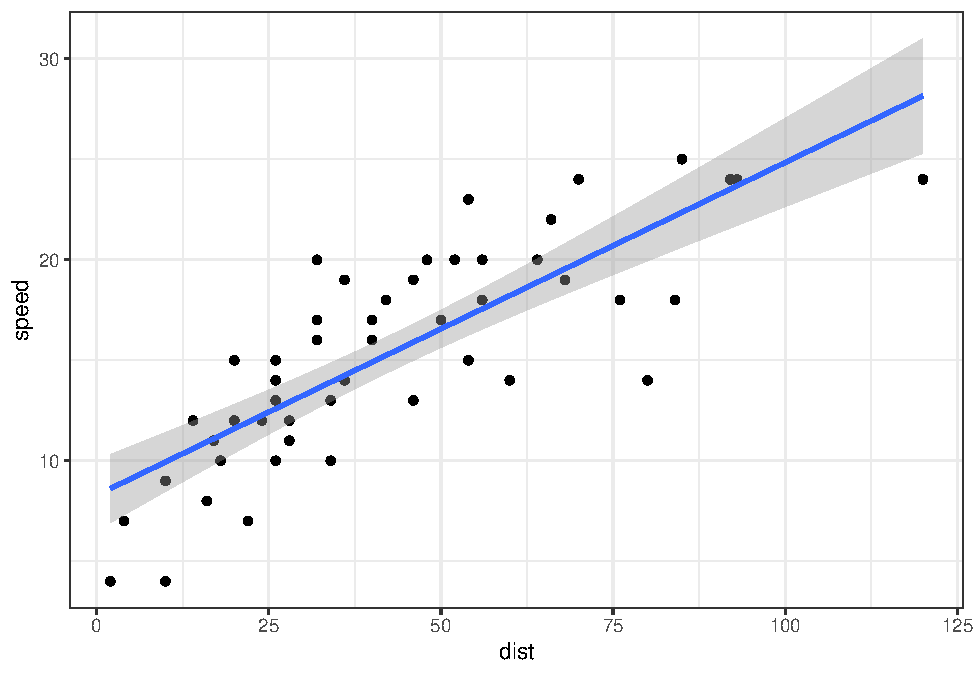
\includegraphics[width=0.8\linewidth]{InfBayes_files/figure-latex/unnamed-chunk-64-1} \end{center}

\(~\)

\(~\)

Sob a abordagem \emph{bayesiana}, a distribuição Normal-Inversa Gama (\emph{NIG}) é uma priori conjugada para \(\boldsymbol{\theta} = (\boldsymbol{\beta},\sigma^2)\) neste modelo. Assim,
\[(\boldsymbol{\beta},\sigma^2) \sim \textit{NIG}(\boldsymbol{\beta}_0, \boldsymbol{V}_0, a_0, b_0)~.\]

Isto é,

\(\boldsymbol{\beta} | \sigma^2 \sim Normal_p\left(\boldsymbol{\beta}_0,\sigma^2\boldsymbol{V}_0\right)~~\); \(~~ \sigma^2 \sim InvGamma\left(a_0,b_0\right)\)

ou, equivalentemente,

\(\boldsymbol{\beta} \sim T_p\left(2a_0; \boldsymbol{\beta}_0,\frac{b_0 \boldsymbol{V}_0}{a_0}\right) ~~\); \(~~ \sigma^2 | \boldsymbol{\beta} \sim InvGamma\left(a_0 + \frac{p}{2},b_0 + \frac{\left(\boldsymbol{\beta}-\boldsymbol{\beta}_0\right)^T \boldsymbol{V}_0^{-1} \left(\boldsymbol{\beta}-\boldsymbol{\beta}_0\right) }{2}\right)~~\),

com \(\boldsymbol{\beta}_0 \in \mathbb{R}^p\), \(\boldsymbol{V}_0\) matriz simétrica positiva definida e \(a_0, b_0 \in \mathbb{R}_+\).

\(~\)

Então:
\[(\boldsymbol{\beta},\sigma^2)|\boldsymbol{Z} \sim \textit{NIG}(\boldsymbol{\beta}_1, \boldsymbol{V}_1, a_1, b_1)\]

com
\(\boldsymbol{\beta}_1 = \boldsymbol{V}_1\left(\boldsymbol{V}_0^{-1}\boldsymbol{\beta}_0 + \boldsymbol{X}^T\boldsymbol{X} \hat{\boldsymbol{\beta}}\right) ~~\); \(~~ \boldsymbol{V}_1 = \left(\boldsymbol{V}_0^{-1} + \boldsymbol{X}^T\boldsymbol{X}\right)^{-1}~~\);
\(a_1 = a_0+\frac{n}{2} ~~\); \(~~ b_1 = b_0 + \frac{\boldsymbol{\beta}_0^T\boldsymbol{V}_0^{-1}\boldsymbol{\beta}_0 + \boldsymbol{Y}^T\boldsymbol{Y} - \boldsymbol{\beta}_1^T\boldsymbol{V}_1^{-1}\boldsymbol{\beta}_1}{2}\).

\(~\)

\textbf{Observação.} Uma das maneiras de representar falta de informação nesse contexto é utilizar a priori de Jeffreys, \(f(\boldsymbol \theta) = \Big|~\mathcal{I}(\boldsymbol \theta)~\Big|^{1/2} \propto 1/\sigma^2\). Nesse caso, distribuição a posteriori é \[(\boldsymbol{\beta},\sigma^2)\Big|\boldsymbol{Z} \sim \textit{NIG}\left(\hat{\boldsymbol{\beta}}, \left(\boldsymbol{X}^T\boldsymbol{X}\right)^{-1}, \dfrac{n-p}{2}, \dfrac{(n-p)s^2}{2}\right)~.\]

\(~\)

\(~\)

\textbf{Exemplo.} Considere que, a priori, \((\boldsymbol{\beta},\sigma^2) \sim \textit{NIG}\left(\boldsymbol{\beta}_0, \boldsymbol{V}_0, a_0, b_0\right)\), com \(~\boldsymbol{\beta}_0 = \left[\begin{array}{c} 0\\0\end{array}\right]~\);
\(~\boldsymbol{V}_0 = \left[\begin{array}{cc} 100 & 0\\ 0 & 100\end{array}\right] ~\); \(~a_0 = 3~\); \(~b_0 = 100~\).

A seguir são apresentadas as distribuições marginais dos parâmetros, a distribuição marginal e as regiões HPD bivariadas do parâmetro \(\boldsymbol{\beta}\).

\begin{Shaded}
\begin{Highlighting}[]
\NormalTok{x =}\StringTok{ }\NormalTok{cars}\OperatorTok{$}\NormalTok{dist   }\CommentTok{# variável resposta}
\NormalTok{y =}\StringTok{ }\NormalTok{cars}\OperatorTok{$}\NormalTok{speed  }\CommentTok{# variável explicativa}
\NormalTok{n =}\StringTok{ }\KeywordTok{length}\NormalTok{(x)   }\CommentTok{# n=50}
\NormalTok{X =}\StringTok{ }\KeywordTok{cbind}\NormalTok{(}\DecValTok{1}\NormalTok{,x)  }\CommentTok{# Matrix de planejamento}
\NormalTok{p =}\StringTok{ }\KeywordTok{ncol}\NormalTok{(X)     }\CommentTok{# p=2}
\NormalTok{g =}\StringTok{ }\NormalTok{n}\OperatorTok{-}\NormalTok{p         }\CommentTok{# gl=48}
\NormalTok{beta_est =}\StringTok{ }\KeywordTok{solve}\NormalTok{(}\KeywordTok{t}\NormalTok{(X)}\OperatorTok\NormalTok{X)}\OperatorTok\NormalTok{(}\KeywordTok{t}\NormalTok{(X)}\OperatorTok\NormalTok{y) }\CommentTok{# (-17.6, 3.9)}
\NormalTok{sigma_est =}
\StringTok{  }\KeywordTok{as.double}\NormalTok{(}\KeywordTok{t}\NormalTok{(y}\OperatorTok{-}\NormalTok{X}\OperatorTok\NormalTok{beta_est)}\OperatorTok\NormalTok{(y}\OperatorTok{-}\NormalTok{X}\OperatorTok\NormalTok{beta_est)}\OperatorTok{/}\NormalTok{(n}\OperatorTok{-}\NormalTok{p)) }\CommentTok{#236.5}
\NormalTok{beta0 =}\StringTok{ }\KeywordTok{c}\NormalTok{(}\DecValTok{0}\NormalTok{,}\DecValTok{0}\NormalTok{)                     }\CommentTok{# média priori betas}
\NormalTok{V0 =}\StringTok{ }\KeywordTok{matrix}\NormalTok{(}\KeywordTok{c}\NormalTok{(}\DecValTok{100}\NormalTok{,}\DecValTok{0}\NormalTok{,}\DecValTok{0}\NormalTok{,}\DecValTok{100}\NormalTok{),}\DataTypeTok{ncol=}\DecValTok{2}\NormalTok{) }\CommentTok{# matriz de escala beta}
\NormalTok{a0 =}\StringTok{ }\DecValTok{3}                             \CommentTok{# priori sigma}
\NormalTok{b0 =}\StringTok{ }\DecValTok{100}                           \CommentTok{# priori sigma}
\CommentTok{# parâmetros da posteriori}
\NormalTok{V1 =}\StringTok{ }\KeywordTok{solve}\NormalTok{(}\KeywordTok{solve}\NormalTok{(V0) }\OperatorTok{+}\StringTok{ }\KeywordTok{t}\NormalTok{(X)}\OperatorTok\NormalTok{X)}
\NormalTok{beta1 =}\StringTok{ }\NormalTok{V1}\OperatorTok\NormalTok{(}\KeywordTok{solve}\NormalTok{(V0)}\OperatorTok\NormalTok{beta0 }\OperatorTok{+}\StringTok{ }\KeywordTok{t}\NormalTok{(X)}\OperatorTok\NormalTok{X}\OperatorTok\NormalTok{beta_est)}
\NormalTok{a1 =}\StringTok{ }\NormalTok{a0 }\OperatorTok{+}\StringTok{ }\NormalTok{n}\OperatorTok{/}\DecValTok{2}
\NormalTok{b1 =}\StringTok{ }\KeywordTok{as.double}\NormalTok{(b0 }\OperatorTok{+}\StringTok{ }\NormalTok{(}\KeywordTok{t}\NormalTok{(beta0)}\OperatorTok\KeywordTok{solve}\NormalTok{(V0)}\OperatorTok\NormalTok{beta0 }\OperatorTok{+}\StringTok{ }\KeywordTok{t}\NormalTok{(y)}\OperatorTok\NormalTok{y }\OperatorTok{-}\StringTok{ }\KeywordTok{t}\NormalTok{(beta1)}\OperatorTok\KeywordTok{solve}\NormalTok{(V1)}\OperatorTok\NormalTok{beta1)}\OperatorTok{/}\DecValTok{2}\NormalTok{)}
\NormalTok{V =}\StringTok{ }\NormalTok{b1}\OperatorTok{*}\NormalTok{V1}\OperatorTok{/}\NormalTok{a1 }\CommentTok{# Matrix de escala da posteriori marginal de beta}

\NormalTok{beta1lim=}\KeywordTok{c}\NormalTok{(beta1[}\DecValTok{1}\NormalTok{]}\OperatorTok{-}\KeywordTok{qt}\NormalTok{(}\FloatTok{0.9999}\NormalTok{,}\DecValTok{2}\OperatorTok{*}\NormalTok{a1)}\OperatorTok{*}\KeywordTok{sqrt}\NormalTok{(V[}\DecValTok{1}\NormalTok{,}\DecValTok{1}\NormalTok{]),beta1[}\DecValTok{1}\NormalTok{]}\OperatorTok{+}\KeywordTok{qt}\NormalTok{(}\FloatTok{0.9999}\NormalTok{,}\DecValTok{2}\OperatorTok{*}\NormalTok{a1)}\OperatorTok{*}\KeywordTok{sqrt}\NormalTok{(V[}\DecValTok{1}\NormalTok{,}\DecValTok{1}\NormalTok{]))}
\NormalTok{beta2lim=}\KeywordTok{c}\NormalTok{(beta1[}\DecValTok{2}\NormalTok{]}\OperatorTok{-}\KeywordTok{qt}\NormalTok{(}\FloatTok{0.9999}\NormalTok{,}\DecValTok{2}\OperatorTok{*}\NormalTok{a1)}\OperatorTok{*}\KeywordTok{sqrt}\NormalTok{(V[}\DecValTok{2}\NormalTok{,}\DecValTok{2}\NormalTok{]),beta1[}\DecValTok{2}\NormalTok{]}\OperatorTok{+}\KeywordTok{qt}\NormalTok{(}\FloatTok{0.9999}\NormalTok{,}\DecValTok{2}\OperatorTok{*}\NormalTok{a1)}\OperatorTok{*}\KeywordTok{sqrt}\NormalTok{(V[}\DecValTok{2}\NormalTok{,}\DecValTok{2}\NormalTok{]))}
\NormalTok{sigma2lim=}\KeywordTok{c}\NormalTok{(extraDistr}\OperatorTok{::}\KeywordTok{qinvgamma}\NormalTok{(}\FloatTok{0.0001}\NormalTok{,a1,b1),extraDistr}\OperatorTok{::}\KeywordTok{qinvgamma}\NormalTok{(}\FloatTok{0.9999}\NormalTok{,a1,b1))}

\NormalTok{b1plot <-}\StringTok{ }\KeywordTok{ggplot}\NormalTok{(}\KeywordTok{data.frame}\NormalTok{(}\DataTypeTok{x=}\NormalTok{beta1lim), }\KeywordTok{aes}\NormalTok{(}\DataTypeTok{x=}\NormalTok{x), }\DataTypeTok{colour =} \StringTok{"0.Posterior"}\NormalTok{) }\OperatorTok{+}
\StringTok{  }\KeywordTok{stat_function}\NormalTok{(}\DataTypeTok{fun =}\NormalTok{ mnormt}\OperatorTok{::}\NormalTok{dmt,}\DataTypeTok{args =} \KeywordTok{list}\NormalTok{(}\DataTypeTok{mean =}\NormalTok{ beta1[}\DecValTok{1}\NormalTok{], }\DataTypeTok{S =}\NormalTok{ V[}\DecValTok{1}\NormalTok{,}\DecValTok{1}\NormalTok{], }\DataTypeTok{df=}\DecValTok{2}\OperatorTok{*}\NormalTok{a1)) }\OperatorTok{+}
\StringTok{  }\KeywordTok{theme_bw}\NormalTok{() }\OperatorTok{+}\StringTok{ }\KeywordTok{xlab}\NormalTok{(}\KeywordTok{expression}\NormalTok{(beta[}\DecValTok{1}\NormalTok{])) }\OperatorTok{+}\StringTok{ }\KeywordTok{ylab}\NormalTok{(}\StringTok{"Posterior"}\NormalTok{)}
\NormalTok{b2plot <-}\StringTok{ }\KeywordTok{ggplot}\NormalTok{(}\KeywordTok{data.frame}\NormalTok{(}\DataTypeTok{x=}\NormalTok{beta2lim), }\KeywordTok{aes}\NormalTok{(}\DataTypeTok{x=}\NormalTok{x), }\DataTypeTok{colour =} \StringTok{"0.Posterior"}\NormalTok{) }\OperatorTok{+}
\StringTok{  }\KeywordTok{stat_function}\NormalTok{(}\DataTypeTok{fun =}\NormalTok{ mnormt}\OperatorTok{::}\NormalTok{dmt, }\DataTypeTok{args =} \KeywordTok{list}\NormalTok{(}\DataTypeTok{mean =}\NormalTok{ beta1[}\DecValTok{2}\NormalTok{], }\DataTypeTok{S =}\NormalTok{ V[}\DecValTok{2}\NormalTok{,}\DecValTok{2}\NormalTok{], }\DataTypeTok{df=}\DecValTok{2}\OperatorTok{*}\NormalTok{a1)) }\OperatorTok{+}
\StringTok{  }\KeywordTok{theme_bw}\NormalTok{() }\OperatorTok{+}\StringTok{ }\KeywordTok{xlab}\NormalTok{(}\KeywordTok{expression}\NormalTok{(beta[}\DecValTok{2}\NormalTok{])) }\OperatorTok{+}\StringTok{ }\KeywordTok{ylab}\NormalTok{(}\StringTok{"Posterior"}\NormalTok{)}
\NormalTok{s2plot <-}\StringTok{ }\KeywordTok{ggplot}\NormalTok{(}\KeywordTok{data.frame}\NormalTok{(}\DataTypeTok{x=}\NormalTok{sigma2lim),}\KeywordTok{aes}\NormalTok{(}\DataTypeTok{x=}\NormalTok{x), }\DataTypeTok{colour =} \StringTok{"0.Posterior"}\NormalTok{)}\OperatorTok{+}
\StringTok{  }\KeywordTok{stat_function}\NormalTok{(}\DataTypeTok{fun =}\NormalTok{ extraDistr}\OperatorTok{::}\NormalTok{dinvgamma, }\DataTypeTok{args =} \KeywordTok{list}\NormalTok{(}\DataTypeTok{alpha =}\NormalTok{ a1, }\DataTypeTok{beta =}\NormalTok{ b1)) }\OperatorTok{+}
\StringTok{  }\KeywordTok{theme_bw}\NormalTok{() }\OperatorTok{+}\StringTok{ }\KeywordTok{xlab}\NormalTok{(}\KeywordTok{expression}\NormalTok{(sigma}\OperatorTok{^}\DecValTok{2}\NormalTok{)) }\OperatorTok{+}\StringTok{ }\KeywordTok{ylab}\NormalTok{(}\StringTok{"Posterior"}\NormalTok{)}
\KeywordTok{multiplot}\NormalTok{(b1plot,b2plot,s2plot)}
\end{Highlighting}
\end{Shaded}

\begin{center}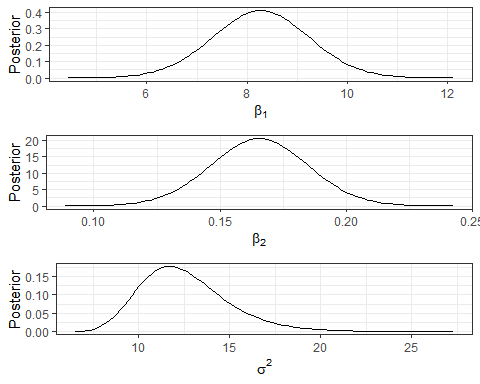
\includegraphics[width=0.8\linewidth]{InfBayes_files/figure-latex/unnamed-chunk-65-1} \end{center}

\begin{Shaded}
\begin{Highlighting}[]
\CommentTok{# posteriori marginal bivariada dos betas}
\NormalTok{posterior <-}\StringTok{ }\ControlFlowTok{function}\NormalTok{(theta0,theta1) \{ }\KeywordTok{apply}\NormalTok{(}\KeywordTok{cbind}\NormalTok{(theta0,theta1),}\DecValTok{1}\NormalTok{,}\ControlFlowTok{function}\NormalTok{(w)\{ mnormt}\OperatorTok{::}\KeywordTok{dmt}\NormalTok{(w, }\DataTypeTok{mean=}\KeywordTok{c}\NormalTok{(beta1), }\DataTypeTok{S=}\NormalTok{V, }\DataTypeTok{df=}\DecValTok{2}\OperatorTok{*}\NormalTok{a1)  \}) \}}
\CommentTok{# Gráfico da posteriori marginal bivariada dos betas}
\NormalTok{grx <-}\StringTok{ }\KeywordTok{seq}\NormalTok{(beta1lim[}\DecValTok{1}\NormalTok{], beta1lim[}\DecValTok{2}\NormalTok{],}\DataTypeTok{length.out=}\DecValTok{200}\NormalTok{)}
\NormalTok{gry <-}\StringTok{ }\KeywordTok{seq}\NormalTok{(beta2lim[}\DecValTok{1}\NormalTok{], beta2lim[}\DecValTok{2}\NormalTok{],}\DataTypeTok{length.out=}\DecValTok{200}\NormalTok{)}
\NormalTok{z1 <-}\StringTok{ }\KeywordTok{outer}\NormalTok{(grx,gry,posterior)}
\CommentTok{#persp(grx,gry,z1)}
\NormalTok{plotly}\OperatorTok{::}\KeywordTok{plot_ly}\NormalTok{(}\DataTypeTok{alpha=}\FloatTok{0.1}\NormalTok{) }\OperatorTok
\StringTok{  }\NormalTok{plotly}\OperatorTok{::}\KeywordTok{add_surface}\NormalTok{(}\DataTypeTok{x=}\NormalTok{grx, }\DataTypeTok{y=}\NormalTok{gry, }\DataTypeTok{z=}\KeywordTok{t}\NormalTok{(z1), }\DataTypeTok{colorscale =} \KeywordTok{list}\NormalTok{(}\KeywordTok{c}\NormalTok{(}\DecValTok{0}\NormalTok{,}\StringTok{'#BA52ED'}\NormalTok{), }\KeywordTok{c}\NormalTok{(}\DecValTok{1}\NormalTok{,}\StringTok{'#FCB040'}\NormalTok{)), }\DataTypeTok{showscale =} \OtherTok{FALSE}\NormalTok{)}
\end{Highlighting}
\end{Shaded}

\begin{center}
\includegraphics[width=0.8\linewidth]{InfBayes_files/figure-latex/unnamed-chunk-66-1} \end{center}

\begin{Shaded}
\begin{Highlighting}[]
\CommentTok{# Curvas de Probabilidade}
\NormalTok{l =}\StringTok{ }\KeywordTok{c}\NormalTok{(}\FloatTok{0.1}\NormalTok{,}\FloatTok{0.3}\NormalTok{,}\FloatTok{0.5}\NormalTok{,}\FloatTok{0.8}\NormalTok{,}\FloatTok{0.9}\NormalTok{,}\FloatTok{0.95}\NormalTok{,}\FloatTok{0.99}\NormalTok{)}
\NormalTok{z1v =}\StringTok{ }\KeywordTok{sort}\NormalTok{(}\KeywordTok{as.vector}\NormalTok{(z1),}\DataTypeTok{decreasing =} \OtherTok{TRUE}\NormalTok{)}
\NormalTok{v1 <-}\StringTok{ }\NormalTok{z1v}\OperatorTok{/}\KeywordTok{sum}\NormalTok{(z1v)}
\NormalTok{a=}\DecValTok{0}\NormalTok{; j=}\DecValTok{1}\NormalTok{; l1=}\OtherTok{NULL}
\ControlFlowTok{for}\NormalTok{(i }\ControlFlowTok{in} \DecValTok{1}\OperatorTok{:}\KeywordTok{length}\NormalTok{(v1)) \{}
\NormalTok{  a <-}\StringTok{ }\NormalTok{a}\OperatorTok{+}\NormalTok{v1[i]}
  \ControlFlowTok{if}\NormalTok{(j}\OperatorTok{<=}\KeywordTok{length}\NormalTok{(l) }\OperatorTok{&}\StringTok{ }\NormalTok{a}\OperatorTok{>}\NormalTok{l[j]) \{}
\NormalTok{    l1 <-}\StringTok{ }\KeywordTok{c}\NormalTok{(l1,z1v[i}\DecValTok{-1}\NormalTok{])}
\NormalTok{    j <-}\StringTok{ }\NormalTok{j}\OperatorTok{+}\DecValTok{1}
\NormalTok{  \}}
\NormalTok{\}}
\KeywordTok{contour}\NormalTok{(grx,gry,z1,}\DataTypeTok{col=}\KeywordTok{colors}\NormalTok{()[}\DecValTok{455}\NormalTok{],}\DataTypeTok{main=}\StringTok{"Regiões HPD para os Betas"}\NormalTok{,}\DataTypeTok{xlab=}\KeywordTok{expression}\NormalTok{(beta[}\DecValTok{1}\NormalTok{]),}\DataTypeTok{ylab=}\KeywordTok{expression}\NormalTok{(beta[}\DecValTok{2}\NormalTok{]),}\DataTypeTok{levels=}\NormalTok{l1,}\DataTypeTok{labels=}\NormalTok{l)}
\KeywordTok{points}\NormalTok{(beta1[}\DecValTok{1}\NormalTok{],beta1[}\DecValTok{2}\NormalTok{],}\DataTypeTok{col=}\StringTok{"darkred"}\NormalTok{,}\DataTypeTok{pch=}\DecValTok{16}\NormalTok{,}\DataTypeTok{cex=}\FloatTok{0.5}\NormalTok{)}
\end{Highlighting}
\end{Shaded}

\begin{center}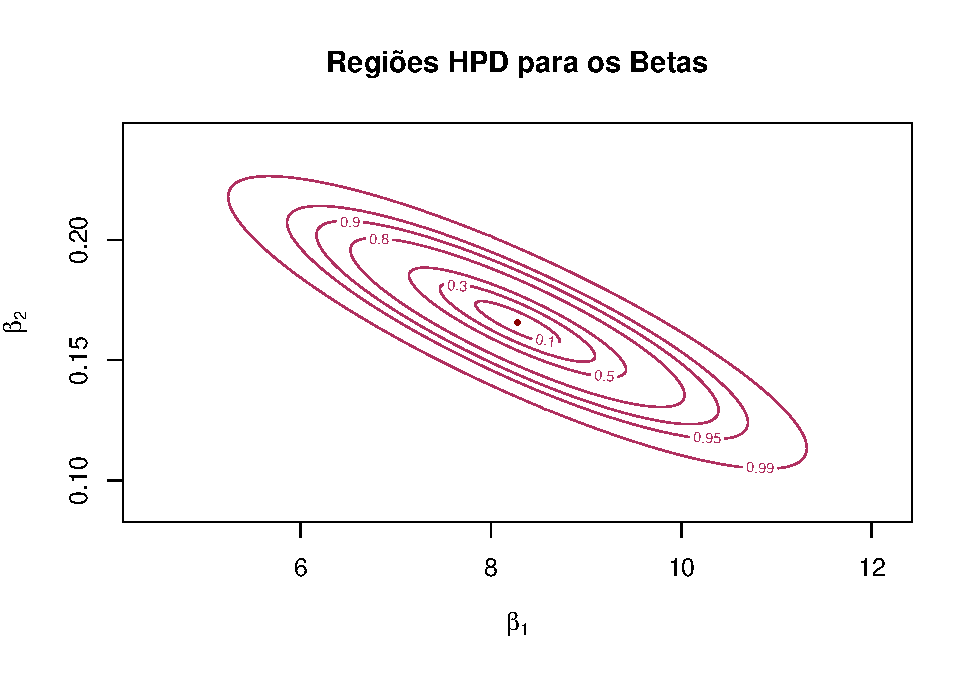
\includegraphics[width=0.8\linewidth]{InfBayes_files/figure-latex/unnamed-chunk-67-1} \end{center}

\(~\)

\(~\)

\hypertarget{laplaces-demon}{%
\subsection{Laplace's Demon}\label{laplaces-demon}}

LaplacesDemon é uma biblioteca do R que oferece diversos algoritimos implementados de MCMC, permitindo fazer Inferência Bayesiana aproximada. Os algoritimos de MCMC disponíveis são

\begin{enumerate}
\def\labelenumi{\arabic{enumi}.}
\tightlist
\item
  Automated Factor Slice Sampler (AFSS)
\item
  Adaptive Directional Metropolis-within-Gibbs (ADMG)
\item
  Adaptive Griddy-Gibbs (AGG)
\item
  Adaptive Hamiltonian Monte Carlo (AHMC)
\item
  Adaptive Metropolis (AM)
\item
  Adaptive Metropolis-within-Gibbs (AMWG)
\item
  Adaptive-Mixture Metropolis (AMM)
\item
  Affine-Invariant Ensemble Sampler (AIES)
\item
  Componentwise Hit-And-Run Metropolis (CHARM)
\item
  Delayed Rejection Adaptive Metropolis (DRAM)
\item
  Delayed Rejection Metropolis (DRM)
\item
  Differential Evolution Markov Chain (DEMC)
\item
  Elliptical Slice Sampler (ESS)
\item
  Gibbs Sampler (Gibbs)
\item
  Griddy-Gibbs (GG)
\item
  Hamiltonian Monte Carlo (HMC)
\item
  Hamiltonian Monte Carlo with Dual-Averaging (HMCDA)
\item
  Hit-And-Run Metropolis (HARM)
\item
  Independence Metropolis (IM)
\item
  Interchain Adaptation (INCA)
\item
  Metropolis-Adjusted Langevin Algorithm (MALA)
\item
  Metropolis-Coupled Markov Chain Monte Carlo (MCMCMC)
\item
  Metropolis-within-Gibbs (MWG)
\item
  Multiple-Try Metropolis (MTM)
\item
  No-U-Turn Sampler (NUTS)
\item
  Oblique Hyperrectangle Slice Sampler (OHSS)
\item
  Preconditioned Crank-Nicolson (pCN)
\item
  Random Dive Metropolis-Hastings (RDMH)
\item
  Random-Walk Metropolis (RWM)
\item
  Reflective Slice Sampler (RSS)
\item
  Refractive Sampler (Refractive)
\item
  Reversible-Jump (RJ)
\item
  Robust Adaptive Metropolis (RAM)
\item
  Sequential Adaptive Metropolis-within-Gibbs (SAMWG)
\item
  Sequential Metropolis-within-Gibbs (SMWG)
\item
  Slice Sampler (Slice)
\item
  Stochastic Gradient Langevin Dynamics (SGLD)
\item
  Tempered Hamiltonian Monte Carlo (THMC)
\item
  t-walk (twalk)
\item
  Univariate Eigenvector Slice Sampler (UESS)
\item
  Updating Sequential Adaptive Metropolis-within-Gibbs (USAMWG)
\item
  Updating Sequential Metropolis-within-Gibbs (USMWG)
\end{enumerate}

\url{https://cran.r-project.org/web/packages/LaplacesDemon/vignettes/BayesianInference.pdf}

\url{https://cran.r-project.org/web/packages/LaplacesDemon/vignettes/LaplacesDemonTutorial.pdf}

\url{https://cran.r-project.org/web/packages/LaplacesDemon/vignettes/Examples.pdf}

\url{https://cran.r-project.org/web/packages/LaplacesDemon/LaplacesDemon.pdf}

\(~\)

\begin{itemize}
\tightlist
\item
  Especificação do modelo
\end{itemize}

\begin{Shaded}
\begin{Highlighting}[]
\KeywordTok{require}\NormalTok{(LaplacesDemon)}

\NormalTok{parm.names=}\KeywordTok{as.parm.names}\NormalTok{(}\KeywordTok{list}\NormalTok{(}\DataTypeTok{beta=}\KeywordTok{rep}\NormalTok{(}\DecValTok{0}\NormalTok{,p), }\DataTypeTok{sigma2=}\DecValTok{0}\NormalTok{))}
\NormalTok{pos.beta=}\KeywordTok{grep}\NormalTok{(}\StringTok{"beta"}\NormalTok{, parm.names)}
\NormalTok{pos.sigma=}\KeywordTok{grep}\NormalTok{(}\StringTok{"sigma2"}\NormalTok{, parm.names)}

\NormalTok{MyData <-}\StringTok{ }\KeywordTok{list}\NormalTok{(}\DataTypeTok{J=}\NormalTok{p, }\DataTypeTok{X=}\NormalTok{X, }\DataTypeTok{y=}\NormalTok{y, }\DataTypeTok{mon.names=}\StringTok{"LP"}\NormalTok{,}
  \DataTypeTok{parm.names=}\NormalTok{parm.names,}\DataTypeTok{pos.beta=}\NormalTok{pos.beta,}\DataTypeTok{pos.sigma=}\NormalTok{pos.sigma)}

\NormalTok{Model <-}\StringTok{ }\ControlFlowTok{function}\NormalTok{(parm, Data)}
\NormalTok{\{}
  \CommentTok{### Parameters}
\NormalTok{  beta <-}\StringTok{ }\NormalTok{parm[Data}\OperatorTok{$}\NormalTok{pos.beta]}
\NormalTok{  sigma2 <-}\StringTok{ }\KeywordTok{interval}\NormalTok{(parm[Data}\OperatorTok{$}\NormalTok{pos.sigma], }\FloatTok{1e-100}\NormalTok{, }\OtherTok{Inf}\NormalTok{)}
\NormalTok{  parm[Data}\OperatorTok{$}\NormalTok{pos.sigma] <-}\StringTok{ }\NormalTok{sigma2}
  \CommentTok{### Log-Prior}
\NormalTok{  sigma.prior <-}\StringTok{ }\KeywordTok{dinvgamma}\NormalTok{(sigma2, a0, b0, }\DataTypeTok{log=}\OtherTok{TRUE}\NormalTok{)}
\NormalTok{  beta.prior <-}\StringTok{ }\KeywordTok{dmvn}\NormalTok{(beta, beta0, sigma2}\OperatorTok{*}\NormalTok{V0, }\DataTypeTok{log=}\OtherTok{TRUE}\NormalTok{)}
  \CommentTok{### Log-Likelihood}
\NormalTok{  mu <-}\StringTok{ }\KeywordTok{tcrossprod}\NormalTok{(Data}\OperatorTok{$}\NormalTok{X, }\KeywordTok{t}\NormalTok{(beta))}
\NormalTok{  LL <-}\StringTok{ }\KeywordTok{sum}\NormalTok{(}\KeywordTok{dnormv}\NormalTok{(Data}\OperatorTok{$}\NormalTok{y, mu, sigma2, }\DataTypeTok{log=}\OtherTok{TRUE}\NormalTok{))}
  \CommentTok{### Log-Posterior}
\NormalTok{  LP <-}\StringTok{ }\NormalTok{LL }\OperatorTok{+}\StringTok{ }\NormalTok{beta.prior }\OperatorTok{+}\StringTok{ }\NormalTok{sigma.prior}
\NormalTok{  Modelout <-}\StringTok{ }\KeywordTok{list}\NormalTok{(}\DataTypeTok{LP=}\NormalTok{LP, }\DataTypeTok{Dev=}\OperatorTok{-}\DecValTok{2}\OperatorTok{*}\NormalTok{LL, }\DataTypeTok{Monitor=}\NormalTok{LP,}
                   \DataTypeTok{yhat=}\KeywordTok{rnorm}\NormalTok{(}\KeywordTok{length}\NormalTok{(mu), mu, sigma2), }\DataTypeTok{parm=}\NormalTok{parm)}
  \KeywordTok{return}\NormalTok{(Modelout)}
\NormalTok{\}}

\NormalTok{Initial.Values <-}\StringTok{ }\KeywordTok{c}\NormalTok{(beta_est,sigma_est)}

\NormalTok{burnin <-}\StringTok{ }\DecValTok{2000}
\NormalTok{thin <-}\StringTok{ }\DecValTok{3}
\NormalTok{N=(}\DecValTok{2000}\OperatorTok{+}\NormalTok{burnin)}\OperatorTok{*}\NormalTok{thin}
\end{Highlighting}
\end{Shaded}

\begin{center}\rule{0.5\linewidth}{0.5pt}\end{center}

\begin{itemize}
\tightlist
\item
  \textbf{Exemplo 1:} Metropolis-within-Gibbs (MWG)
\end{itemize}

\begin{Shaded}
\begin{Highlighting}[]
\KeywordTok{set.seed}\NormalTok{(}\DecValTok{666}\NormalTok{)}
\NormalTok{Fit1 <-}\StringTok{ }\KeywordTok{LaplacesDemon}\NormalTok{(Model, }\DataTypeTok{Data=}\NormalTok{MyData, Initial.Values,}
  \DataTypeTok{Covar=}\OtherTok{NULL}\NormalTok{, }\DataTypeTok{Iterations=}\NormalTok{N, }\DataTypeTok{Status=}\NormalTok{N}\OperatorTok{/}\DecValTok{5}\NormalTok{, }\DataTypeTok{Thinning=}\NormalTok{thin,}
  \DataTypeTok{Algorithm=}\StringTok{"MWG"}\NormalTok{, }\DataTypeTok{Specs=}\OtherTok{NULL}\NormalTok{)}
\end{Highlighting}
\end{Shaded}

\begin{verbatim}
## 
## Laplace's Demon was called on Tue Nov 03 14:52:16 2020
## 
## Performing initial checks...
## Algorithm: Metropolis-within-Gibbs 
## 
## Laplace's Demon is beginning to update...
## Iteration: 2400,   Proposal: Componentwise,   LP: -146.2
## Iteration: 4800,   Proposal: Componentwise,   LP: -147.2
## Iteration: 7200,   Proposal: Componentwise,   LP: -142.7
## Iteration: 9600,   Proposal: Componentwise,   LP: -143.5
## Iteration: 12000,   Proposal: Componentwise,   LP: -145.1
## 
## Assessing Stationarity
## Assessing Thinning and ESS
## Creating Summaries
## Estimating Log of the Marginal Likelihood
## Creating Output
## 
## Laplace's Demon has finished.
\end{verbatim}

\begin{Shaded}
\begin{Highlighting}[]
\CommentTok{#names(Fit1)}
\KeywordTok{print}\NormalTok{(Fit1)}
\end{Highlighting}
\end{Shaded}

\begin{verbatim}
## Call:
## LaplacesDemon(Model = Model, Data = MyData, Initial.Values = Initial.Values, 
##     Covar = NULL, Iterations = N, Status = N/5, Thinning = thin, 
##     Algorithm = "MWG", Specs = NULL)
## 
## Acceptance Rate: 0.35375
## Algorithm: Metropolis-within-Gibbs
## Covariance Matrix: (NOT SHOWN HERE; diagonal shown instead)
##  beta[1]  beta[2]   sigma2 
## 1.890044 1.890044 1.890044 
## 
## Covariance (Diagonal) History: (NOT SHOWN HERE)
## Deviance Information Criterion (DIC):
##          All Stationary
## Dbar 258.781    259.440
## pD     4.338      4.237
## DIC  263.119    263.677
## Initial Values:
## [1] 8.2839056 0.1655676 9.9587760
## 
## Iterations: 12000
## Log(Marginal Likelihood): -126.8415
## Minutes of run-time: 0.3
## Model: (NOT SHOWN HERE)
## Monitor: (NOT SHOWN HERE)
## Parameters (Number of): 3
## Posterior1: (NOT SHOWN HERE)
## Posterior2: (NOT SHOWN HERE)
## Recommended Burn-In of Thinned Samples: 3200
## Recommended Burn-In of Un-thinned Samples: 9600
## Recommended Thinning: 36
## Specs: (NOT SHOWN HERE)
## Status is displayed every 2400 iterations
## Summary1: (SHOWN BELOW)
## Summary2: (SHOWN BELOW)
## Thinned Samples: 4000
## Thinning: 3
## 
## 
## Summary of All Samples
##                  Mean         SD        MCSE       ESS           LB
## beta[1]     8.2478022 0.88164035 0.094717679  24.80187    6.6527588
## beta[2]     0.1665176 0.01702535 0.003042654  12.48151    0.1240373
## sigma2     12.5840386 2.48412045 0.125660593 830.27788    8.7682617
## Deviance  258.7813640 2.94533567 0.202218161 136.68013  255.0038715
## LP       -143.5465138 1.23958817 0.087107901 109.45812 -146.5361533
##                Median           UB
## beta[1]     8.2225293   10.1866171
## beta[2]     0.1655676    0.1937371
## sigma2     12.2724404   18.2059419
## Deviance  258.1752506  265.5673438
## LP       -143.2451510 -142.1163971
## 
## 
## Summary of Stationary Samples
##                  Mean         SD        MCSE        ESS           LB
## beta[1]     8.9659139 1.01640981 0.264577460   6.932756    6.5707408
## beta[2]     0.1498047 0.02004864 0.007080864   3.675837    0.1240373
## sigma2     12.4235537 2.25114323 0.223124198 148.522644    8.9164125
## Deviance  259.4399279 2.91101586 0.562252817  35.086016  255.3738557
## LP       -143.8933516 1.24169010 0.191055588  27.276956 -146.8229317
##                Median           UB
## beta[1]     9.0304813   10.6078726
## beta[2]     0.1504279    0.1937371
## sigma2     12.0978375   17.6632608
## Deviance  258.9769661  265.8590137
## LP       -143.6581852 -142.1644366
\end{verbatim}

\begin{Shaded}
\begin{Highlighting}[]
\NormalTok{Post1 <-}\StringTok{ }\KeywordTok{data.frame}\NormalTok{(Fit1}\OperatorTok{$}\NormalTok{Posterior1,}\DataTypeTok{Algorithm=}\StringTok{"1.MWG"}\NormalTok{)}
\KeywordTok{colnames}\NormalTok{(Post1) <-}\StringTok{ }\KeywordTok{c}\NormalTok{(}\StringTok{"beta1"}\NormalTok{,}\StringTok{"beta2"}\NormalTok{,}\StringTok{"sigma2"}\NormalTok{,}\StringTok{"Algorithm"}\NormalTok{)}
\CommentTok{#head(Post1)}
\KeywordTok{plot}\NormalTok{(Fit1, }\DataTypeTok{BurnIn=}\DecValTok{0}\NormalTok{, MyData, }\DataTypeTok{PDF=}\OtherTok{FALSE}\NormalTok{, }\DataTypeTok{Parms=}\OtherTok{NULL}\NormalTok{)}
\end{Highlighting}
\end{Shaded}

\begin{center}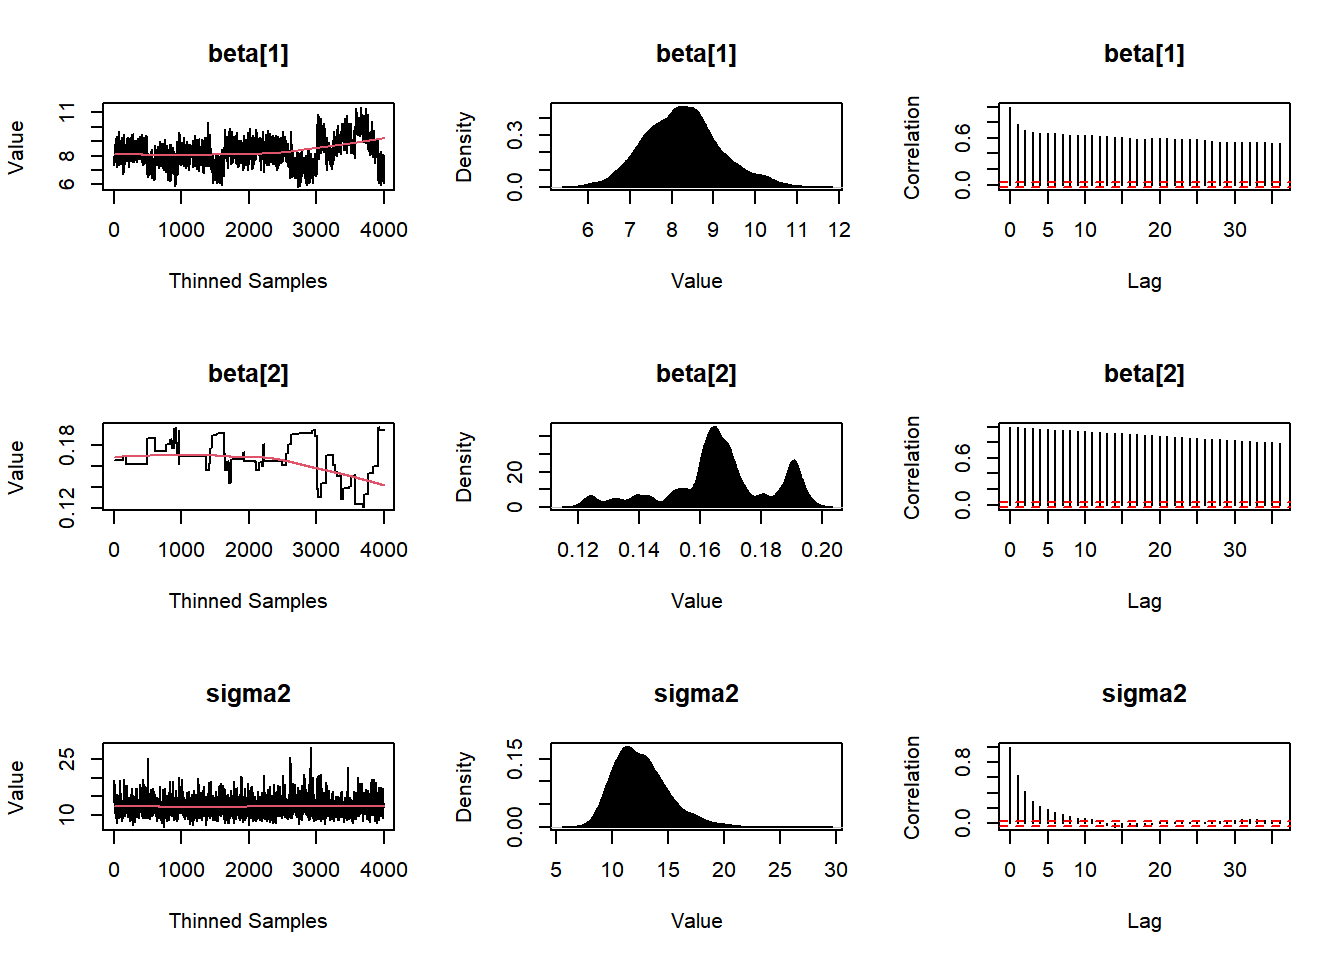
\includegraphics[width=0.8\linewidth]{InfBayes_files/figure-latex/unnamed-chunk-69-1} \end{center}

\begin{Shaded}
\begin{Highlighting}[]
\CommentTok{#plot(Fit1, BurnIn=burnin, MyData, PDF=FALSE, Parms=NULL)}
\end{Highlighting}
\end{Shaded}

\begin{center}\includegraphics[width=0.8\linewidth]{InfBayes_files/figure-latex/unnamed-chunk-69-2} \end{center}

\begin{center}\rule{0.5\linewidth}{0.5pt}\end{center}

\begin{itemize}
\tightlist
\item
  \textbf{Exemplo 2:} Adaptative Metropolis-within-Gibbs (MWG)
\end{itemize}

\begin{Shaded}
\begin{Highlighting}[]
\KeywordTok{set.seed}\NormalTok{(}\DecValTok{666}\NormalTok{)}
\NormalTok{Fit2 <-}\StringTok{ }\KeywordTok{LaplacesDemon}\NormalTok{(Model, }\DataTypeTok{Data=}\NormalTok{MyData, Initial.Values,}
  \DataTypeTok{Covar=}\OtherTok{NULL}\NormalTok{, }\DataTypeTok{Iterations=}\NormalTok{N, }\DataTypeTok{Status=}\NormalTok{N}\OperatorTok{/}\DecValTok{5}\NormalTok{, }\DataTypeTok{Thinning=}\NormalTok{thin,}
  \DataTypeTok{Algorithm=}\StringTok{"AMWG"}\NormalTok{, }\DataTypeTok{Specs=}\OtherTok{NULL}\NormalTok{)}
\end{Highlighting}
\end{Shaded}

\begin{verbatim}
## 
## Laplace's Demon was called on Tue Nov 03 14:52:38 2020
## 
## Performing initial checks...
## Algorithm: Adaptive Metropolis-within-Gibbs 
## 
## Laplace's Demon is beginning to update...
## Iteration: 2400,   Proposal: Componentwise,   LP: -145.3
## Iteration: 4800,   Proposal: Componentwise,   LP: -143
## Iteration: 7200,   Proposal: Componentwise,   LP: -144.1
## Iteration: 9600,   Proposal: Componentwise,   LP: -143.1
## Iteration: 12000,   Proposal: Componentwise,   LP: -146.2
## 
## Assessing Stationarity
## Assessing Thinning and ESS
## Creating Summaries
## Creating Output
## 
## Laplace's Demon has finished.
\end{verbatim}

\begin{Shaded}
\begin{Highlighting}[]
\CommentTok{#names(Fit2)}
\CommentTok{#print(Fit2)}

\NormalTok{Post2 <-}\StringTok{ }\KeywordTok{data.frame}\NormalTok{(Fit2}\OperatorTok{$}\NormalTok{Posterior1,}\DataTypeTok{Algorithm=}\StringTok{"2.AMWG"}\NormalTok{)}
\KeywordTok{colnames}\NormalTok{(Post2) <-}\StringTok{ }\KeywordTok{c}\NormalTok{(}\StringTok{"beta1"}\NormalTok{,}\StringTok{"beta2"}\NormalTok{,}\StringTok{"sigma2"}\NormalTok{,}\StringTok{"Algorithm"}\NormalTok{)}
\CommentTok{#head(Post2)}

\CommentTok{#plot(Fit2, BurnIn=burnin, MyData, PDF=FALSE, Parms=NULL)}
\KeywordTok{plot}\NormalTok{(Fit2, }\DataTypeTok{BurnIn=}\DecValTok{0}\NormalTok{, MyData, }\DataTypeTok{PDF=}\OtherTok{FALSE}\NormalTok{, }\DataTypeTok{Parms=}\OtherTok{NULL}\NormalTok{)}
\end{Highlighting}
\end{Shaded}

\begin{center}\includegraphics[width=0.8\linewidth]{InfBayes_files/figure-latex/unnamed-chunk-70-1} \end{center}

\begin{center}\includegraphics[width=0.8\linewidth]{InfBayes_files/figure-latex/unnamed-chunk-70-2} \end{center}

\begin{Shaded}
\begin{Highlighting}[]
\NormalTok{Post <-}\StringTok{ }\KeywordTok{rbind}\NormalTok{(Post1,Post2)}
\NormalTok{b1plot <-}\StringTok{ }\KeywordTok{ggplot}\NormalTok{(Post) }\OperatorTok{+}
\StringTok{  }\KeywordTok{stat_function}\NormalTok{(}\KeywordTok{aes}\NormalTok{(}\DataTypeTok{colour=}\StringTok{"0.Posterior"}\NormalTok{), }\DataTypeTok{fun =}\NormalTok{ mnormt}\OperatorTok{::}\NormalTok{dmt,}\DataTypeTok{args =} \KeywordTok{list}\NormalTok{(}\DataTypeTok{mean =}\NormalTok{ beta1[}\DecValTok{1}\NormalTok{], }\DataTypeTok{S =}\NormalTok{ V[}\DecValTok{1}\NormalTok{,}\DecValTok{1}\NormalTok{], }\DataTypeTok{df=}\DecValTok{2}\OperatorTok{*}\NormalTok{a1)) }\OperatorTok{+}
\StringTok{  }\KeywordTok{geom_density}\NormalTok{(}\KeywordTok{aes}\NormalTok{(beta1, }\DataTypeTok{colour =}\NormalTok{ Algorithm)) }\OperatorTok{+}\StringTok{ }\KeywordTok{theme_bw}\NormalTok{() }\OperatorTok{+}
\StringTok{  }\KeywordTok{xlab}\NormalTok{(}\KeywordTok{expression}\NormalTok{(beta[}\DecValTok{1}\NormalTok{])) }\OperatorTok{+}\StringTok{ }\KeywordTok{ylab}\NormalTok{(}\StringTok{"Posterior"}\NormalTok{) }\OperatorTok{+}\StringTok{ }\KeywordTok{labs}\NormalTok{(}\DataTypeTok{colour =} \StringTok{"Method"}\NormalTok{)}
\NormalTok{b2plot <-}\StringTok{ }\KeywordTok{ggplot}\NormalTok{(Post) }\OperatorTok{+}
\StringTok{  }\KeywordTok{stat_function}\NormalTok{(}\KeywordTok{aes}\NormalTok{(}\DataTypeTok{colour=}\StringTok{"0.Posterior"}\NormalTok{), }\DataTypeTok{fun =}\NormalTok{ mnormt}\OperatorTok{::}\NormalTok{dmt, }\DataTypeTok{args =} \KeywordTok{list}\NormalTok{(}\DataTypeTok{mean =}\NormalTok{ beta1[}\DecValTok{2}\NormalTok{], }\DataTypeTok{S =}\NormalTok{ V[}\DecValTok{2}\NormalTok{,}\DecValTok{2}\NormalTok{], }\DataTypeTok{df=}\DecValTok{2}\OperatorTok{*}\NormalTok{a1)) }\OperatorTok{+}
\StringTok{  }\KeywordTok{geom_density}\NormalTok{(}\KeywordTok{aes}\NormalTok{(beta2, }\DataTypeTok{colour =}\NormalTok{ Algorithm)) }\OperatorTok{+}\StringTok{ }\KeywordTok{theme_bw}\NormalTok{() }\OperatorTok{+}
\StringTok{  }\KeywordTok{xlab}\NormalTok{(}\KeywordTok{expression}\NormalTok{(beta[}\DecValTok{2}\NormalTok{])) }\OperatorTok{+}\StringTok{ }\KeywordTok{ylab}\NormalTok{(}\StringTok{"Posterior"}\NormalTok{) }\OperatorTok{+}\StringTok{ }\KeywordTok{labs}\NormalTok{(}\DataTypeTok{colour =} \StringTok{"Method"}\NormalTok{)}
\NormalTok{s2plot <-}\StringTok{ }\KeywordTok{ggplot}\NormalTok{(Post)}\OperatorTok{+}
\StringTok{  }\KeywordTok{stat_function}\NormalTok{(}\KeywordTok{aes}\NormalTok{(}\DataTypeTok{colour=}\StringTok{"0.Posterior"}\NormalTok{), }\DataTypeTok{fun =}\NormalTok{ extraDistr}\OperatorTok{::}\NormalTok{dinvgamma, }\DataTypeTok{args =} \KeywordTok{list}\NormalTok{(}\DataTypeTok{alpha =}\NormalTok{ a1, }\DataTypeTok{beta =}\NormalTok{ b1)) }\OperatorTok{+}
\StringTok{  }\KeywordTok{geom_density}\NormalTok{(}\KeywordTok{aes}\NormalTok{(sigma2, }\DataTypeTok{colour =}\NormalTok{ Algorithm)) }\OperatorTok{+}\StringTok{ }\KeywordTok{theme_bw}\NormalTok{() }\OperatorTok{+}
\StringTok{  }\KeywordTok{xlab}\NormalTok{(}\KeywordTok{expression}\NormalTok{(sigma}\OperatorTok{^}\DecValTok{2}\NormalTok{)) }\OperatorTok{+}\StringTok{ }\KeywordTok{ylab}\NormalTok{(}\StringTok{"Posterior"}\NormalTok{) }\OperatorTok{+}\StringTok{ }\KeywordTok{labs}\NormalTok{(}\DataTypeTok{colour =} \StringTok{"Method"}\NormalTok{)}
\KeywordTok{multiplot}\NormalTok{(b1plot,b2plot,s2plot)}
\end{Highlighting}
\end{Shaded}

\begin{center}\includegraphics[width=0.8\linewidth]{InfBayes_files/figure-latex/unnamed-chunk-71-1} \end{center}

\begin{center}\rule{0.5\linewidth}{0.5pt}\end{center}

\begin{itemize}
\tightlist
\item
  \textbf{Exemplo 3:} Consort e Automated Factor Slice Sampler (AFSS)
\end{itemize}

\begin{Shaded}
\begin{Highlighting}[]
\KeywordTok{Consort}\NormalTok{(Fit2)}
\end{Highlighting}
\end{Shaded}

\begin{verbatim}
## 
## #############################################################
## # Consort with Laplace's Demon                              #
## #############################################################
## Call:
## LaplacesDemon(Model = Model, Data = MyData, Initial.Values = Initial.Values, 
##     Covar = NULL, Iterations = N, Status = N/5, Thinning = thin, 
##     Algorithm = "AMWG", Specs = NULL)
## 
## Acceptance Rate: 0.34264
## Algorithm: Adaptive Metropolis-within-Gibbs
## Covariance Matrix: (NOT SHOWN HERE; diagonal shown instead)
##    beta[1]    beta[2]     sigma2 
## 1.17679178 0.02838563 9.45831955 
## 
## Covariance (Diagonal) History: (NOT SHOWN HERE)
## Deviance Information Criterion (DIC):
##          All Stationary
## Dbar 258.957    258.957
## pD     4.957      4.957
## DIC  263.915    263.915
## Initial Values:
## [1] 8.2839056 0.1655676 9.9587760
## 
## Iterations: 12000
## Log(Marginal Likelihood): NA
## Minutes of run-time: 0.3
## Model: (NOT SHOWN HERE)
## Monitor: (NOT SHOWN HERE)
## Parameters (Number of): 3
## Posterior1: (NOT SHOWN HERE)
## Posterior2: (NOT SHOWN HERE)
## Recommended Burn-In of Thinned Samples: 0
## Recommended Burn-In of Un-thinned Samples: 0
## Recommended Thinning: 105
## Specs: (NOT SHOWN HERE)
## Status is displayed every 2400 iterations
## Summary1: (SHOWN BELOW)
## Summary2: (SHOWN BELOW)
## Thinned Samples: 4000
## Thinning: 3
## 
## 
## Summary of All Samples
##                  Mean         SD        MCSE       ESS           LB
## beta[1]     8.2386566 0.97788924 0.085914819  151.0105    6.1651888
## beta[2]     0.1661183 0.01903241 0.002099194  209.2080    0.1294318
## sigma2     12.5980978 2.45984860 0.071949821 1784.2000    8.7806779
## Deviance  258.9573762 3.14870026 0.163068368  595.3985  255.1347857
## LP       -143.6311506 1.33506450 0.072413145  530.5654 -147.0582460
##                Median           UB
## beta[1]     8.2641629   10.1040670
## beta[2]     0.1655676    0.2078131
## sigma2     12.3274919   18.1748415
## Deviance  258.2440979  266.8653177
## LP       -143.2679823 -142.1324005
## 
## 
## Summary of Stationary Samples
##                  Mean         SD        MCSE       ESS           LB
## beta[1]     8.2386566 0.97788924 0.085914819  151.0105    6.1651888
## beta[2]     0.1661183 0.01903241 0.002099194  209.2080    0.1294318
## sigma2     12.5980978 2.45984860 0.071949821 1784.2000    8.7806779
## Deviance  258.9573762 3.14870026 0.163068368  595.3985  255.1347857
## LP       -143.6311506 1.33506450 0.072413145  530.5654 -147.0582460
##                Median           UB
## beta[1]     8.2641629   10.1040670
## beta[2]     0.1655676    0.2078131
## sigma2     12.3274919   18.1748415
## Deviance  258.2440979  266.8653177
## LP       -143.2679823 -142.1324005
## 
## Demonic Suggestion
## 
## Due to the combination of the following conditions,
## 
## 1. Adaptive Metropolis-within-Gibbs
## 2. The acceptance rate (0.3426389) is within the interval [0.15,0.5].
## 3. At least one target MCSE is >= 6.27% of its marginal posterior
##    standard deviation.
## 4. Each target distribution has an effective sample size (ESS)
##    of at least 100.
## 5. Each target distribution became stationary by
##    1 iteration.
## 
## Quantiles of Absolute Posterior1 Correlation:
##         0%        25%        50%        75%       100% 
## 0.02856704 0.03170699 0.85367854 1.00000000 1.00000000 
## 
## Possibly excessive posterior correlation for a componentwise algorithm.
## 
## WARNING: Diminishing adaptation did not occur.
##          A new algorithm will be suggested.
## 
## Laplace's Demon has not been appeased, and suggests
## copy/pasting the following R code into the R console,
## and running it.
## 
## Initial.Values <- as.initial.values(Fit2)
## Fit2 <- LaplacesDemon(Model, Data=MyData, Initial.Values,
##      Covar=Fit2$Covar, Iterations=420000, Status=40000, Thinning=105,
##      Algorithm="AFSS", Specs=list(A=Inf, B=NULL, m=100,
##      n=0, w=1))
## 
## Laplace's Demon is finished consorting.
\end{verbatim}

\begin{Shaded}
\begin{Highlighting}[]
\NormalTok{Initial.Values <-}\StringTok{ }\KeywordTok{as.initial.values}\NormalTok{(Fit2)}

\KeywordTok{set.seed}\NormalTok{(}\DecValTok{666}\NormalTok{)}
\NormalTok{Fit3 <-}\StringTok{ }\KeywordTok{LaplacesDemon}\NormalTok{(Model, }\DataTypeTok{Data=}\NormalTok{MyData, Initial.Values,}
     \DataTypeTok{Covar=}\OtherTok{NULL}\NormalTok{, }\DataTypeTok{Iterations=}\NormalTok{N, }\DataTypeTok{Status=}\NormalTok{N}\OperatorTok{/}\DecValTok{5}\NormalTok{, }\DataTypeTok{Thinning=}\NormalTok{thin,}
     \DataTypeTok{Algorithm=}\StringTok{"AFSS"}\NormalTok{, }\DataTypeTok{Specs=}\KeywordTok{list}\NormalTok{(}\DataTypeTok{A=}\OtherTok{Inf}\NormalTok{, }\DataTypeTok{B=}\OtherTok{NULL}\NormalTok{, }\DataTypeTok{m=}\DecValTok{100}\NormalTok{,}\DataTypeTok{n=}\DecValTok{0}\NormalTok{, }\DataTypeTok{w=}\DecValTok{1}\NormalTok{))}
\end{Highlighting}
\end{Shaded}

\begin{verbatim}
## 
## Laplace's Demon was called on Tue Nov 03 14:53:24 2020
## 
## Performing initial checks...
## Algorithm: Automated Factor Slice Sampler 
## 
## Laplace's Demon is beginning to update...
## 
## Eigendecomposition will occur every 120 iterations.
## 
## Iteration: 2400,   Proposal: Multivariate,   LP: -142.1
## Iteration: 4800,   Proposal: Multivariate,   LP: -144.2
## Iteration: 7200,   Proposal: Multivariate,   LP: -145.2
## Iteration: 9600,   Proposal: Multivariate,   LP: -144.1
## Iteration: 12000,   Proposal: Multivariate,   LP: -142.5
## 
## Assessing Stationarity
## Assessing Thinning and ESS
## Creating Summaries
## Estimating Log of the Marginal Likelihood
## Creating Output
## 
## Laplace's Demon has finished.
\end{verbatim}

\begin{Shaded}
\begin{Highlighting}[]
\NormalTok{Post3 <-}\StringTok{ }\KeywordTok{data.frame}\NormalTok{(Fit3}\OperatorTok{$}\NormalTok{Posterior1,}\DataTypeTok{Algorithm=}\StringTok{"3.AFSS"}\NormalTok{)}
\KeywordTok{colnames}\NormalTok{(Post3) <-}\StringTok{ }\KeywordTok{c}\NormalTok{(}\StringTok{"beta1"}\NormalTok{,}\StringTok{"beta2"}\NormalTok{,}\StringTok{"sigma2"}\NormalTok{,}\StringTok{"Algorithm"}\NormalTok{)}
\KeywordTok{plot}\NormalTok{(Fit3, }\DataTypeTok{BurnIn=}\DecValTok{0}\NormalTok{, MyData, }\DataTypeTok{PDF=}\OtherTok{FALSE}\NormalTok{, }\DataTypeTok{Parms=}\OtherTok{NULL}\NormalTok{)}
\end{Highlighting}
\end{Shaded}

\begin{center}\includegraphics[width=0.8\linewidth]{InfBayes_files/figure-latex/unnamed-chunk-72-1} \end{center}

\begin{center}\includegraphics[width=0.8\linewidth]{InfBayes_files/figure-latex/unnamed-chunk-72-2} \end{center}

\begin{Shaded}
\begin{Highlighting}[]
\NormalTok{Post <-}\StringTok{ }\KeywordTok{rbind}\NormalTok{(Post1,Post2,Post3)}
\NormalTok{b1plot <-}\StringTok{ }\KeywordTok{ggplot}\NormalTok{(Post) }\OperatorTok{+}
\StringTok{  }\KeywordTok{stat_function}\NormalTok{(}\KeywordTok{aes}\NormalTok{(}\DataTypeTok{colour=}\StringTok{"0.Posterior"}\NormalTok{), }\DataTypeTok{fun =}\NormalTok{ mnormt}\OperatorTok{::}\NormalTok{dmt,}\DataTypeTok{args =} \KeywordTok{list}\NormalTok{(}\DataTypeTok{mean =}\NormalTok{ beta1[}\DecValTok{1}\NormalTok{], }\DataTypeTok{S =}\NormalTok{ V[}\DecValTok{1}\NormalTok{,}\DecValTok{1}\NormalTok{], }\DataTypeTok{df=}\DecValTok{2}\OperatorTok{*}\NormalTok{a1)) }\OperatorTok{+}
\StringTok{  }\KeywordTok{geom_density}\NormalTok{(}\KeywordTok{aes}\NormalTok{(beta1, }\DataTypeTok{colour =}\NormalTok{ Algorithm)) }\OperatorTok{+}\StringTok{ }\KeywordTok{theme_bw}\NormalTok{() }\OperatorTok{+}
\StringTok{  }\KeywordTok{xlab}\NormalTok{(}\KeywordTok{expression}\NormalTok{(beta[}\DecValTok{1}\NormalTok{])) }\OperatorTok{+}\StringTok{ }\KeywordTok{ylab}\NormalTok{(}\StringTok{"Posterior"}\NormalTok{) }\OperatorTok{+}\StringTok{ }\KeywordTok{labs}\NormalTok{(}\DataTypeTok{colour =} \StringTok{"Method"}\NormalTok{)}
\NormalTok{b2plot <-}\StringTok{ }\KeywordTok{ggplot}\NormalTok{(Post) }\OperatorTok{+}
\StringTok{  }\KeywordTok{stat_function}\NormalTok{(}\KeywordTok{aes}\NormalTok{(}\DataTypeTok{colour=}\StringTok{"0.Posterior"}\NormalTok{), }\DataTypeTok{fun =}\NormalTok{ mnormt}\OperatorTok{::}\NormalTok{dmt, }\DataTypeTok{args =} \KeywordTok{list}\NormalTok{(}\DataTypeTok{mean =}\NormalTok{ beta1[}\DecValTok{2}\NormalTok{], }\DataTypeTok{S =}\NormalTok{ V[}\DecValTok{2}\NormalTok{,}\DecValTok{2}\NormalTok{], }\DataTypeTok{df=}\DecValTok{2}\OperatorTok{*}\NormalTok{a1)) }\OperatorTok{+}
\StringTok{  }\KeywordTok{geom_density}\NormalTok{(}\KeywordTok{aes}\NormalTok{(beta2, }\DataTypeTok{colour =}\NormalTok{ Algorithm)) }\OperatorTok{+}\StringTok{ }\KeywordTok{theme_bw}\NormalTok{() }\OperatorTok{+}
\StringTok{  }\KeywordTok{xlab}\NormalTok{(}\KeywordTok{expression}\NormalTok{(beta[}\DecValTok{2}\NormalTok{])) }\OperatorTok{+}\StringTok{ }\KeywordTok{ylab}\NormalTok{(}\StringTok{"Posterior"}\NormalTok{) }\OperatorTok{+}\StringTok{ }\KeywordTok{labs}\NormalTok{(}\DataTypeTok{colour =} \StringTok{"Method"}\NormalTok{)}
\NormalTok{s2plot <-}\StringTok{ }\KeywordTok{ggplot}\NormalTok{(Post)}\OperatorTok{+}
\StringTok{  }\KeywordTok{stat_function}\NormalTok{(}\KeywordTok{aes}\NormalTok{(}\DataTypeTok{colour=}\StringTok{"0.Posterior"}\NormalTok{), }\DataTypeTok{fun =}\NormalTok{ extraDistr}\OperatorTok{::}\NormalTok{dinvgamma, }\DataTypeTok{args =} \KeywordTok{list}\NormalTok{(}\DataTypeTok{alpha =}\NormalTok{ a1, }\DataTypeTok{beta =}\NormalTok{ b1)) }\OperatorTok{+}
\StringTok{  }\KeywordTok{geom_density}\NormalTok{(}\KeywordTok{aes}\NormalTok{(sigma2, }\DataTypeTok{colour =}\NormalTok{ Algorithm)) }\OperatorTok{+}\StringTok{ }\KeywordTok{theme_bw}\NormalTok{() }\OperatorTok{+}
\StringTok{  }\KeywordTok{xlab}\NormalTok{(}\KeywordTok{expression}\NormalTok{(sigma}\OperatorTok{^}\DecValTok{2}\NormalTok{)) }\OperatorTok{+}\StringTok{ }\KeywordTok{ylab}\NormalTok{(}\StringTok{"Posterior"}\NormalTok{) }\OperatorTok{+}\StringTok{ }\KeywordTok{labs}\NormalTok{(}\DataTypeTok{colour =} \StringTok{"Method"}\NormalTok{)}
\KeywordTok{multiplot}\NormalTok{(b1plot,b2plot,s2plot)}
\end{Highlighting}
\end{Shaded}

\begin{center}\includegraphics[width=0.8\linewidth]{InfBayes_files/figure-latex/unnamed-chunk-73-1} \end{center}

\begin{Shaded}
\begin{Highlighting}[]
\KeywordTok{p.interval}\NormalTok{(Post3}\OperatorTok{$}\NormalTok{beta1, }\DataTypeTok{HPD=}\OtherTok{FALSE}\NormalTok{, }\DataTypeTok{MM=}\OtherTok{FALSE}\NormalTok{, }\DataTypeTok{plot=}\OtherTok{TRUE}\NormalTok{)}
\end{Highlighting}
\end{Shaded}

\begin{center}\includegraphics[width=0.8\linewidth]{InfBayes_files/figure-latex/unnamed-chunk-74-1} \end{center}

\begin{verbatim}
##         Lower  Upper
## [1,] 6.383021 10.175
## attr(,"Probability.Interval")
## [1] 0.95
\end{verbatim}

\begin{Shaded}
\begin{Highlighting}[]
\KeywordTok{set.seed}\NormalTok{(}\DecValTok{666}\NormalTok{)}
\NormalTok{S0 <-}\StringTok{ }\KeywordTok{as.matrix}\NormalTok{(extraDistr}\OperatorTok{::}\KeywordTok{rinvgamma}\NormalTok{(N}\OperatorTok{/}\NormalTok{thin}\OperatorTok{-}\NormalTok{burnin,a1,b1))}
\NormalTok{M0 <-}\StringTok{ }\KeywordTok{apply}\NormalTok{(S0,}\DecValTok{1}\NormalTok{,}\ControlFlowTok{function}\NormalTok{(s)\{mnormt}\OperatorTok{::}\KeywordTok{rmnorm}\NormalTok{(}\DecValTok{1}\NormalTok{,}\DataTypeTok{mean=}\NormalTok{beta1,}\DataTypeTok{varcov=}\NormalTok{s}\OperatorTok{*}\NormalTok{V1)\})}
\NormalTok{Post0 <-}\StringTok{ }\KeywordTok{data.frame}\NormalTok{(}\KeywordTok{t}\NormalTok{(M0),S0,}\StringTok{"0.Posterior"}\NormalTok{)}
\KeywordTok{colnames}\NormalTok{(Post0) <-}\StringTok{ }\KeywordTok{c}\NormalTok{(}\StringTok{"beta1"}\NormalTok{,}\StringTok{"beta2"}\NormalTok{,}\StringTok{"sigma2"}\NormalTok{,}\StringTok{"Algorithm"}\NormalTok{)}
\NormalTok{Post =}\StringTok{ }\KeywordTok{rbind}\NormalTok{(Post0,Post1,Post2,Post3)}
\KeywordTok{ggplot}\NormalTok{(Post) }\OperatorTok{+}\StringTok{ }\KeywordTok{theme_bw}\NormalTok{() }\OperatorTok{+}
\StringTok{  }\KeywordTok{geom_point}\NormalTok{(}\KeywordTok{aes}\NormalTok{(beta1,beta2,}\DataTypeTok{colour=}\NormalTok{Algorithm), }\DataTypeTok{shape=}\DecValTok{1}\NormalTok{) }\OperatorTok{+}
\StringTok{  }\KeywordTok{facet_wrap}\NormalTok{(Algorithm }\OperatorTok{~}\StringTok{ }\NormalTok{.)}
\end{Highlighting}
\end{Shaded}

\begin{center}\includegraphics[width=0.8\linewidth]{InfBayes_files/figure-latex/unnamed-chunk-74-2} \end{center}

\begin{center}\rule{0.5\linewidth}{0.5pt}\end{center}

\hypertarget{stan}{%
\subsection{Stan}\label{stan}}

O Stan é uma plataforma de modelagem estatística de alto desempenho. Em particular, permite fazer inferência bayesiana usando o método de Monte Carlo Hamiltoniano (HMC) e a variação No-U-Turn Sampler (NUTS). Esses recursos convergem para distribuições alvo de altas dimensões muito mais rapidamente que métodos mais simples, como o amostrador de Gibbs ou outras variações do método de Metropolis-Hastings. A da linguagem utilizada é independente da plataforma e existem bibliotecas para R (\texttt{rstan}) e Python.

\url{https://mc-stan.org/}

\(~\)

\textbf{Voltando ao Exemplo}

\begin{Shaded}
\begin{Highlighting}[]
\KeywordTok{library}\NormalTok{(rstan)}
\CommentTok{# Parametros do método}
\NormalTok{Initial.Values <-}\StringTok{ }\KeywordTok{c}\NormalTok{(beta_est,sigma_est)}
\NormalTok{burnin <-}\StringTok{ }\DecValTok{2000}
\NormalTok{thin <-}\StringTok{ }\DecValTok{3}
\NormalTok{N=(}\DecValTok{2000}\OperatorTok{+}\NormalTok{burnin)}\OperatorTok{*}\NormalTok{thin}
\CommentTok{# Conjunto de dados}
\NormalTok{stan_data <-}\StringTok{ }\KeywordTok{list}\NormalTok{(}\DataTypeTok{N =}\NormalTok{ n, }\DataTypeTok{J =}\NormalTok{ p, }\DataTypeTok{y =}\NormalTok{ y, }\DataTypeTok{x =}\NormalTok{ X)}

\CommentTok{# Especificação do modelo}
\NormalTok{rs_code <-}\StringTok{ '}
\StringTok{  data \{}
\StringTok{    int<lower=1> N;}
\StringTok{    int<lower=1> J;}
\StringTok{    matrix[N,J] x;}
\StringTok{    vector[N] y;}
\StringTok{  \}}
\StringTok{  parameters \{}
\StringTok{    vector[J] beta;}
\StringTok{    real<lower=0> sigma2;}
\StringTok{  \}}
\StringTok{  model \{}
\StringTok{    sigma2 ~ inv_gamma(3, 100);}
\StringTok{    beta ~ normal(0, sqrt(sigma2*100));}
\StringTok{    y ~ normal(x * beta, sqrt(sigma2));}
\StringTok{\}'}

\NormalTok{stan_mod <-}\StringTok{ }\KeywordTok{stan}\NormalTok{(}\DataTypeTok{model_code =}\NormalTok{ rs_code, }\DataTypeTok{data =}\NormalTok{ stan_data, }\DataTypeTok{init=}\NormalTok{Initial.Values,}
            \DataTypeTok{chains =} \DecValTok{1}\NormalTok{, }\DataTypeTok{iter =}\NormalTok{ N, }\DataTypeTok{warmup =}\NormalTok{ burnin, }\DataTypeTok{thin =}\NormalTok{ thin)}
\end{Highlighting}
\end{Shaded}

\begin{verbatim}
## 
## SAMPLING FOR MODEL '6b158d2712aa5479f81bd408884c9453' NOW (CHAIN 1).
## Chain 1: 
## Chain 1: Gradient evaluation took 0 seconds
## Chain 1: 1000 transitions using 10 leapfrog steps per transition would take 0 seconds.
## Chain 1: Adjust your expectations accordingly!
## Chain 1: 
## Chain 1: 
## Chain 1: Iteration:     1 / 12000 [  0%]  (Warmup)
## Chain 1: Iteration:  1200 / 12000 [ 10%]  (Warmup)
## Chain 1: Iteration:  2001 / 12000 [ 16%]  (Sampling)
## Chain 1: Iteration:  3200 / 12000 [ 26%]  (Sampling)
## Chain 1: Iteration:  4400 / 12000 [ 36%]  (Sampling)
## Chain 1: Iteration:  5600 / 12000 [ 46%]  (Sampling)
## Chain 1: Iteration:  6800 / 12000 [ 56%]  (Sampling)
## Chain 1: Iteration:  8000 / 12000 [ 66%]  (Sampling)
## Chain 1: Iteration:  9200 / 12000 [ 76%]  (Sampling)
## Chain 1: Iteration: 10400 / 12000 [ 86%]  (Sampling)
## Chain 1: Iteration: 11600 / 12000 [ 96%]  (Sampling)
## Chain 1: Iteration: 12000 / 12000 [100%]  (Sampling)
## Chain 1: 
## Chain 1:  Elapsed Time: 0.289 seconds (Warm-up)
## Chain 1:                1.451 seconds (Sampling)
## Chain 1:                1.74 seconds (Total)
## Chain 1:
\end{verbatim}

\begin{Shaded}
\begin{Highlighting}[]
\NormalTok{posterior <-}\StringTok{ }\NormalTok{rstan}\OperatorTok{::}\KeywordTok{extract}\NormalTok{(stan_mod)}
\NormalTok{Post4 <-}\StringTok{ }\KeywordTok{data.frame}\NormalTok{(posterior}\OperatorTok{$}\NormalTok{beta[,}\DecValTok{1}\NormalTok{],posterior}\OperatorTok{$}\NormalTok{beta[,}\DecValTok{2}\NormalTok{],posterior}\OperatorTok{$}\NormalTok{sigma2,}\DataTypeTok{Algorithm=}\StringTok{"4.RStan"}\NormalTok{)}
\KeywordTok{colnames}\NormalTok{(Post4) <-}\StringTok{ }\KeywordTok{c}\NormalTok{(}\StringTok{"beta1"}\NormalTok{,}\StringTok{"beta2"}\NormalTok{,}\StringTok{"sigma2"}\NormalTok{,}\StringTok{"Algorithm"}\NormalTok{)}

\CommentTok{# gráficos posterioris marginais}
\NormalTok{Post <-}\StringTok{ }\KeywordTok{rbind}\NormalTok{(Post3,Post4) }\OperatorTok
\StringTok{  }\KeywordTok{mutate}\NormalTok{(}\DataTypeTok{Algorithm=}\KeywordTok{ifelse}\NormalTok{(Algorithm}\OperatorTok{==}\StringTok{"3.AFSS"}\NormalTok{,}\StringTok{"1.LaplacesDemons"}\NormalTok{,}\StringTok{"2.RStan"}\NormalTok{))}
\NormalTok{b1plot <-}\StringTok{ }\KeywordTok{ggplot}\NormalTok{(Post) }\OperatorTok{+}
\StringTok{  }\KeywordTok{stat_function}\NormalTok{(}\KeywordTok{aes}\NormalTok{(}\DataTypeTok{colour=}\StringTok{"0.Posterior"}\NormalTok{), }\DataTypeTok{fun =}\NormalTok{ mnormt}\OperatorTok{::}\NormalTok{dmt,}\DataTypeTok{args =} \KeywordTok{list}\NormalTok{(}\DataTypeTok{mean =}\NormalTok{ beta1[}\DecValTok{1}\NormalTok{], }\DataTypeTok{S =}\NormalTok{ V[}\DecValTok{1}\NormalTok{,}\DecValTok{1}\NormalTok{], }\DataTypeTok{df=}\DecValTok{2}\OperatorTok{*}\NormalTok{a1)) }\OperatorTok{+}
\StringTok{  }\KeywordTok{geom_density}\NormalTok{(}\KeywordTok{aes}\NormalTok{(beta1, }\DataTypeTok{colour =}\NormalTok{ Algorithm)) }\OperatorTok{+}\StringTok{ }\KeywordTok{theme_bw}\NormalTok{() }\OperatorTok{+}
\StringTok{  }\KeywordTok{xlab}\NormalTok{(}\KeywordTok{expression}\NormalTok{(beta[}\DecValTok{1}\NormalTok{])) }\OperatorTok{+}\StringTok{ }\KeywordTok{ylab}\NormalTok{(}\StringTok{"Posterior"}\NormalTok{) }\OperatorTok{+}\StringTok{ }\KeywordTok{labs}\NormalTok{(}\DataTypeTok{colour =} \StringTok{"Method"}\NormalTok{)}
\NormalTok{b2plot <-}\StringTok{ }\KeywordTok{ggplot}\NormalTok{(Post) }\OperatorTok{+}
\StringTok{  }\KeywordTok{stat_function}\NormalTok{(}\KeywordTok{aes}\NormalTok{(}\DataTypeTok{colour=}\StringTok{"0.Posterior"}\NormalTok{), }\DataTypeTok{fun =}\NormalTok{ mnormt}\OperatorTok{::}\NormalTok{dmt, }\DataTypeTok{args =} \KeywordTok{list}\NormalTok{(}\DataTypeTok{mean =}\NormalTok{ beta1[}\DecValTok{2}\NormalTok{], }\DataTypeTok{S =}\NormalTok{ V[}\DecValTok{2}\NormalTok{,}\DecValTok{2}\NormalTok{], }\DataTypeTok{df=}\DecValTok{2}\OperatorTok{*}\NormalTok{a1)) }\OperatorTok{+}
\StringTok{  }\KeywordTok{geom_density}\NormalTok{(}\KeywordTok{aes}\NormalTok{(beta2, }\DataTypeTok{colour =}\NormalTok{ Algorithm)) }\OperatorTok{+}\StringTok{ }\KeywordTok{theme_bw}\NormalTok{() }\OperatorTok{+}
\StringTok{  }\KeywordTok{xlab}\NormalTok{(}\KeywordTok{expression}\NormalTok{(beta[}\DecValTok{2}\NormalTok{])) }\OperatorTok{+}\StringTok{ }\KeywordTok{ylab}\NormalTok{(}\StringTok{"Posterior"}\NormalTok{) }\OperatorTok{+}\StringTok{ }\KeywordTok{labs}\NormalTok{(}\DataTypeTok{colour =} \StringTok{"Method"}\NormalTok{)}
\NormalTok{s2plot <-}\StringTok{ }\KeywordTok{ggplot}\NormalTok{(Post)}\OperatorTok{+}
\StringTok{  }\KeywordTok{stat_function}\NormalTok{(}\KeywordTok{aes}\NormalTok{(}\DataTypeTok{colour=}\StringTok{"0.Posterior"}\NormalTok{), }\DataTypeTok{fun =}\NormalTok{ extraDistr}\OperatorTok{::}\NormalTok{dinvgamma, }\DataTypeTok{args =} \KeywordTok{list}\NormalTok{(}\DataTypeTok{alpha =}\NormalTok{ a1, }\DataTypeTok{beta =}\NormalTok{ b1)) }\OperatorTok{+}
\StringTok{  }\KeywordTok{geom_density}\NormalTok{(}\KeywordTok{aes}\NormalTok{(sigma2, }\DataTypeTok{colour =}\NormalTok{ Algorithm)) }\OperatorTok{+}\StringTok{ }\KeywordTok{theme_bw}\NormalTok{() }\OperatorTok{+}
\StringTok{  }\KeywordTok{xlab}\NormalTok{(}\KeywordTok{expression}\NormalTok{(sigma}\OperatorTok{^}\DecValTok{2}\NormalTok{)) }\OperatorTok{+}\StringTok{ }\KeywordTok{ylab}\NormalTok{(}\StringTok{"Posterior"}\NormalTok{) }\OperatorTok{+}\StringTok{ }\KeywordTok{labs}\NormalTok{(}\DataTypeTok{colour =} \StringTok{"Method"}\NormalTok{)}
\KeywordTok{multiplot}\NormalTok{(b1plot,b2plot,s2plot)}
\end{Highlighting}
\end{Shaded}

\begin{center}\includegraphics[width=0.8\linewidth]{InfBayes_files/figure-latex/unnamed-chunk-76-1} \end{center}

\begin{Shaded}
\begin{Highlighting}[]
\NormalTok{Post =}\StringTok{ }\KeywordTok{rbind}\NormalTok{(Post0,Post4) }\OperatorTok
\StringTok{  }\KeywordTok{mutate}\NormalTok{(}\DataTypeTok{Algorithm=}\KeywordTok{ifelse}\NormalTok{(Algorithm}\OperatorTok{==}\StringTok{"4.RStan"}\NormalTok{,}\StringTok{"1.RStan"}\NormalTok{,}\StringTok{"0.Posterior"}\NormalTok{))}
\KeywordTok{ggplot}\NormalTok{(Post) }\OperatorTok{+}\StringTok{ }\KeywordTok{theme_bw}\NormalTok{() }\OperatorTok{+}
\StringTok{  }\KeywordTok{geom_point}\NormalTok{(}\KeywordTok{aes}\NormalTok{(beta1,beta2,}\DataTypeTok{colour=}\NormalTok{Algorithm), }\DataTypeTok{shape=}\DecValTok{1}\NormalTok{) }\OperatorTok{+}
\StringTok{  }\KeywordTok{facet_wrap}\NormalTok{(Algorithm }\OperatorTok{~}\StringTok{ }\NormalTok{.)}
\end{Highlighting}
\end{Shaded}

\begin{center}\includegraphics[width=0.8\linewidth]{InfBayes_files/figure-latex/unnamed-chunk-77-1} \end{center}

\(~\)

\begin{Shaded}
\begin{Highlighting}[]
\NormalTok{stan_mod2 <-}\StringTok{ }\KeywordTok{stan}\NormalTok{(}\DataTypeTok{model_code =}\NormalTok{ rs_code, }\DataTypeTok{data =}\NormalTok{ stan_data, }\DataTypeTok{init=}\NormalTok{Initial.Values,}
            \DataTypeTok{chains =} \DecValTok{2}\NormalTok{, }\DataTypeTok{iter =}\NormalTok{ N, }\DataTypeTok{warmup =}\NormalTok{ burnin, }\DataTypeTok{thin =}\NormalTok{ thin)}
\end{Highlighting}
\end{Shaded}

\begin{verbatim}
## 
## SAMPLING FOR MODEL '6b158d2712aa5479f81bd408884c9453' NOW (CHAIN 1).
## Chain 1: 
## Chain 1: Gradient evaluation took 0 seconds
## Chain 1: 1000 transitions using 10 leapfrog steps per transition would take 0 seconds.
## Chain 1: Adjust your expectations accordingly!
## Chain 1: 
## Chain 1: 
## Chain 1: Iteration:     1 / 12000 [  0%]  (Warmup)
## Chain 1: Iteration:  1200 / 12000 [ 10%]  (Warmup)
## Chain 1: Iteration:  2001 / 12000 [ 16%]  (Sampling)
## Chain 1: Iteration:  3200 / 12000 [ 26%]  (Sampling)
## Chain 1: Iteration:  4400 / 12000 [ 36%]  (Sampling)
## Chain 1: Iteration:  5600 / 12000 [ 46%]  (Sampling)
## Chain 1: Iteration:  6800 / 12000 [ 56%]  (Sampling)
## Chain 1: Iteration:  8000 / 12000 [ 66%]  (Sampling)
## Chain 1: Iteration:  9200 / 12000 [ 76%]  (Sampling)
## Chain 1: Iteration: 10400 / 12000 [ 86%]  (Sampling)
## Chain 1: Iteration: 11600 / 12000 [ 96%]  (Sampling)
## Chain 1: Iteration: 12000 / 12000 [100%]  (Sampling)
## Chain 1: 
## Chain 1:  Elapsed Time: 0.278 seconds (Warm-up)
## Chain 1:                0.999 seconds (Sampling)
## Chain 1:                1.277 seconds (Total)
## Chain 1: 
## 
## SAMPLING FOR MODEL '6b158d2712aa5479f81bd408884c9453' NOW (CHAIN 2).
## Chain 2: 
## Chain 2: Gradient evaluation took 0 seconds
## Chain 2: 1000 transitions using 10 leapfrog steps per transition would take 0 seconds.
## Chain 2: Adjust your expectations accordingly!
## Chain 2: 
## Chain 2: 
## Chain 2: Iteration:     1 / 12000 [  0%]  (Warmup)
## Chain 2: Iteration:  1200 / 12000 [ 10%]  (Warmup)
## Chain 2: Iteration:  2001 / 12000 [ 16%]  (Sampling)
## Chain 2: Iteration:  3200 / 12000 [ 26%]  (Sampling)
## Chain 2: Iteration:  4400 / 12000 [ 36%]  (Sampling)
## Chain 2: Iteration:  5600 / 12000 [ 46%]  (Sampling)
## Chain 2: Iteration:  6800 / 12000 [ 56%]  (Sampling)
## Chain 2: Iteration:  8000 / 12000 [ 66%]  (Sampling)
## Chain 2: Iteration:  9200 / 12000 [ 76%]  (Sampling)
## Chain 2: Iteration: 10400 / 12000 [ 86%]  (Sampling)
## Chain 2: Iteration: 11600 / 12000 [ 96%]  (Sampling)
## Chain 2: Iteration: 12000 / 12000 [100%]  (Sampling)
## Chain 2: 
## Chain 2:  Elapsed Time: 0.235 seconds (Warm-up)
## Chain 2:                1.011 seconds (Sampling)
## Chain 2:                1.246 seconds (Total)
## Chain 2:
\end{verbatim}

\begin{Shaded}
\begin{Highlighting}[]
\KeywordTok{library}\NormalTok{(ggmcmc)}
\CommentTok{#ggs(stan_mod2) %>% ggmcmc(., file = "ggmcmc.html")}
\end{Highlighting}
\end{Shaded}

\(~\)

\href{ggmcmc.html}{\textbf{Gráficos ggmcmc}}

\(~\)

\emph{1. Histograma} com as cadeias geradas combinadas.

\begin{Shaded}
\begin{Highlighting}[]
\KeywordTok{ggs}\NormalTok{(stan_mod2) }\OperatorTok\StringTok{ }\KeywordTok{ggs_histogram}\NormalTok{(.)}
\end{Highlighting}
\end{Shaded}

\begin{center}\includegraphics[width=0.8\linewidth]{InfBayes_files/figure-latex/unnamed-chunk-79-1} \end{center}

\emph{2. Gráficos das Densidades} sobrepostos com cores diferentes por cadeia, permite comparar se as cadeias convergiram para distribuições semelhantes.

\begin{Shaded}
\begin{Highlighting}[]
\KeywordTok{ggs}\NormalTok{(stan_mod2) }\OperatorTok\StringTok{ }\KeywordTok{ggs_density}\NormalTok{(.)}
\end{Highlighting}
\end{Shaded}

\begin{center}\includegraphics[width=0.8\linewidth]{InfBayes_files/figure-latex/unnamed-chunk-80-1} \end{center}

\emph{3. Séries Temporais} das cadeias geradas. É esperado que as cadeias geradas apresentem distribuições semelhantes em torno de uma mesma média, indicando assim que atingiu-se a ``estacionariedade''.

\begin{Shaded}
\begin{Highlighting}[]
\KeywordTok{ggs}\NormalTok{(stan_mod2) }\OperatorTok\StringTok{ }\KeywordTok{ggs_traceplot}\NormalTok{(.)}
\end{Highlighting}
\end{Shaded}

\begin{center}\includegraphics[width=0.8\linewidth]{InfBayes_files/figure-latex/unnamed-chunk-81-1} \end{center}

\emph{4. Gráfico de Médias Móveis}. É esperado que as curvas das médias das cadeias geradas se aproximem rapidamente de um mesmo valor.

\begin{Shaded}
\begin{Highlighting}[]
\KeywordTok{ggs}\NormalTok{(stan_mod2) }\OperatorTok\StringTok{ }\KeywordTok{ggs_running}\NormalTok{(.)}
\end{Highlighting}
\end{Shaded}

\begin{center}\includegraphics[width=0.8\linewidth]{InfBayes_files/figure-latex/unnamed-chunk-82-1} \end{center}

\emph{5. Densidades parcial e completa sobrepostas}. Compara a última parte da cadeia (por padrão, os últimos 10\% dos valores, em verde) com a cadeia inteira (em preto). Idealmente, as partes inicial e final da cadeia devem ser amostradas na mesma distribuição alvo, de modo que as densidades sobrepostas devem ser semelhantes.

\begin{Shaded}
\begin{Highlighting}[]
\KeywordTok{ggs}\NormalTok{(stan_mod2) }\OperatorTok\StringTok{ }\KeywordTok{ggs_compare_partial}\NormalTok{(.)}
\end{Highlighting}
\end{Shaded}

\begin{center}\includegraphics[width=0.8\linewidth]{InfBayes_files/figure-latex/unnamed-chunk-83-1} \end{center}

\emph{6. Gráfico de Autocorrelação}. Espera-se alta correlação apenas no primeiro lag. Quando há um comportamento diferente do esperado, deve-se aumentar o tamanho dos saltos (\emph{thin}) entre as observações da cadeia gerada que serão consideradas na amostra final.

\begin{Shaded}
\begin{Highlighting}[]
\KeywordTok{ggs}\NormalTok{(stan_mod2) }\OperatorTok\StringTok{ }\KeywordTok{ggs_autocorrelation}\NormalTok{(.)}
\end{Highlighting}
\end{Shaded}

\begin{center}\includegraphics[width=0.8\linewidth]{InfBayes_files/figure-latex/unnamed-chunk-84-1} \end{center}

\emph{6. Correlação Cruzada}. Quando há alta correlação entre os parâmetros é possível que a convergência da cadeia seja mais lenta.

\begin{Shaded}
\begin{Highlighting}[]
\KeywordTok{ggs}\NormalTok{(stan_mod2) }\OperatorTok\StringTok{ }\KeywordTok{ggs_crosscorrelation}\NormalTok{(.)}
\end{Highlighting}
\end{Shaded}

\begin{center}\includegraphics[width=0.8\linewidth]{InfBayes_files/figure-latex/unnamed-chunk-85-1} \end{center}

\begin{Shaded}
\begin{Highlighting}[]
\KeywordTok{ggs}\NormalTok{(stan_mod2) }\OperatorTok\StringTok{ }\KeywordTok{ggs_pairs}\NormalTok{(., }\DataTypeTok{lower =} \KeywordTok{list}\NormalTok{(}\DataTypeTok{continuous =} \StringTok{"density"}\NormalTok{))}
\end{Highlighting}
\end{Shaded}

\begin{center}\includegraphics[width=0.8\linewidth]{InfBayes_files/figure-latex/unnamed-chunk-86-1} \end{center}

\(~\)

\(~\)

\hypertarget{mlg}{%
\subsection{MLG}\label{mlg}}

O modelos lineares generalizados (MLG) são uma extensão natural dos modelos lineares para casos em que a distribuição da variável resposta não é normal. Como exemplo, vamos considerar o particular caso onde a resposta é binária, conhecido como \emph{regressão logística}.

Considere \(Y_1,\ldots,Y_n\) condicionalmente independentes tais que \(Y_i|\theta_i \sim \textit{Ber}(\theta_i)\), em que \(\theta_i\) é tal que \(\log\left(\dfrac{\theta_i}{1-\theta_i}\right) = \boldsymbol x_i' \boldsymbol\beta\) ou, em outras palavras, \(\theta_i = \dfrac{1}{1+e^{\boldsymbol x_i' \boldsymbol\beta}} = \dfrac{e^{-\boldsymbol x_i' \boldsymbol\beta}}{1+e^{-\boldsymbol x_i' \boldsymbol\beta}}\) com \(\boldsymbol x_i\) as covariáveis da \(i\)-ésima observação e o vetor de parâmetros \(\boldsymbol\beta=(\beta_1,\ldots,\beta_p)\).

\(~\)

\textbf{Exemplo.} Considere as variáveis \emph{vs} (0 = motor em forma de V, 1 = motor reto) e \emph{mpg} (milhas/galão(EUA)) do conjunto de dados \texttt{mtcars} do R. Suponha um modelo de regressão logística para a variável resposta \emph{vs} com a covariável \emph{mpg} em que, a priori, \(\beta_i \sim \textit{Laplace}(0,b_i)\), \(i=1,2\), independentes. Deste modo, a posteriori é dada por

\(f(\boldsymbol\beta | \boldsymbol{y},\boldsymbol{x})\)
\(\propto f(\boldsymbol{y}|\boldsymbol\beta,\boldsymbol{x})f(\boldsymbol\beta)\)
\(\propto \displaystyle\prod_{i=1}^{n} \left(\dfrac{1}{1+e^{\boldsymbol x_i' \boldsymbol\beta}}\right)^{y_i}\left(\dfrac{e^{\boldsymbol x_i' \boldsymbol\beta}}{1+e^{\boldsymbol x_i' \boldsymbol\beta}}\right)^{1-y_i} \prod_{j=1}^{p} \dfrac{1}{2b_i} e^{-\frac{|\beta_i|}{b_i}}\).

\begin{Shaded}
\begin{Highlighting}[]
\KeywordTok{library}\NormalTok{(rstan)}

\NormalTok{dados <-}\StringTok{ }\KeywordTok{as_tibble}\NormalTok{(mtcars)}
\CommentTok{# mpg:  Miles/(US)gallon ;  vs: Engine(0=V-shaped,1=straight)}
\NormalTok{dados }\OperatorTok\StringTok{ }\KeywordTok{ggplot}\NormalTok{(}\KeywordTok{aes}\NormalTok{(}\DataTypeTok{group=}\KeywordTok{as.factor}\NormalTok{(vs),}\DataTypeTok{y=}\NormalTok{mpg,}\DataTypeTok{fill=}\KeywordTok{as.factor}\NormalTok{(vs))) }\OperatorTok{+}
\StringTok{        }\KeywordTok{geom_boxplot}\NormalTok{() }\OperatorTok{+}\StringTok{ }\KeywordTok{scale_fill_discrete}\NormalTok{(}\DataTypeTok{name=}\StringTok{"vs"}\NormalTok{) }\OperatorTok{+}\StringTok{ }\KeywordTok{theme_bw}\NormalTok{()}
\end{Highlighting}
\end{Shaded}

\begin{center}\includegraphics[width=0.8\linewidth]{InfBayes_files/figure-latex/unnamed-chunk-87-1} \end{center}

\begin{Shaded}
\begin{Highlighting}[]
\NormalTok{y <-}\StringTok{ }\NormalTok{dados }\OperatorTok\StringTok{ }\KeywordTok{select}\NormalTok{(vs) }\OperatorTok\StringTok{ }\KeywordTok{pull}\NormalTok{()}
\NormalTok{x <-}\StringTok{ }\NormalTok{dados }\OperatorTok\StringTok{ }\KeywordTok{select}\NormalTok{(mpg) }\OperatorTok\StringTok{ }\KeywordTok{pull}\NormalTok{()}
\NormalTok{n <-}\StringTok{ }\KeywordTok{length}\NormalTok{(y)}
\NormalTok{X <-}\StringTok{ }\KeywordTok{as.matrix}\NormalTok{(}\KeywordTok{cbind}\NormalTok{(}\DecValTok{1}\NormalTok{,x))}
\NormalTok{p <-}\StringTok{ }\KeywordTok{ncol}\NormalTok{(X)}

\NormalTok{stan_data <-}\StringTok{ }\KeywordTok{list}\NormalTok{(}\DataTypeTok{N =}\NormalTok{ n, }\DataTypeTok{J =}\NormalTok{ p, }\DataTypeTok{y =}\NormalTok{ y, }\DataTypeTok{x =}\NormalTok{ X)}

\NormalTok{rs_code <-}\StringTok{ '}
\StringTok{  data \{}
\StringTok{    int<lower=1> N;}
\StringTok{    int<lower=1> J;}
\StringTok{    int<lower=0,upper=1> y[N];}
\StringTok{    matrix[N,J] x;}
\StringTok{  \}}
\StringTok{  parameters \{}
\StringTok{    vector[J] beta;}
\StringTok{  \}}
\StringTok{  model \{}
\StringTok{    beta ~ double_exponential(0, 100);}
\StringTok{    y ~ bernoulli_logit(x * beta);}
\StringTok{  \}'}

\NormalTok{N=}\DecValTok{2000}
\NormalTok{thin=}\DecValTok{10}
\NormalTok{burnin=}\DecValTok{1000}

\NormalTok{stan_log <-}\StringTok{ }\KeywordTok{stan}\NormalTok{(}\DataTypeTok{model_code =}\NormalTok{ rs_code, }\DataTypeTok{data =}\NormalTok{ stan_data, }\DataTypeTok{init =} \KeywordTok{c}\NormalTok{(}\DecValTok{0}\NormalTok{,}\DecValTok{0}\NormalTok{),}
  \DataTypeTok{chains =} \DecValTok{1}\NormalTok{, }\DataTypeTok{iter =}\NormalTok{ N}\OperatorTok{*}\NormalTok{thin, }\DataTypeTok{warmup =}\NormalTok{ burnin, }\DataTypeTok{thin =}\NormalTok{ thin)}
\end{Highlighting}
\end{Shaded}

\begin{verbatim}
## 
## SAMPLING FOR MODEL '6525180a46ff3a51f06bbb110d962a1c' NOW (CHAIN 1).
## Chain 1: 
## Chain 1: Gradient evaluation took 0 seconds
## Chain 1: 1000 transitions using 10 leapfrog steps per transition would take 0 seconds.
## Chain 1: Adjust your expectations accordingly!
## Chain 1: 
## Chain 1: 
## Chain 1: Iteration:     1 / 20000 [  0%]  (Warmup)
## Chain 1: Iteration:  1001 / 20000 [  5%]  (Sampling)
## Chain 1: Iteration:  3000 / 20000 [ 15%]  (Sampling)
## Chain 1: Iteration:  5000 / 20000 [ 25%]  (Sampling)
## Chain 1: Iteration:  7000 / 20000 [ 35%]  (Sampling)
## Chain 1: Iteration:  9000 / 20000 [ 45%]  (Sampling)
## Chain 1: Iteration: 11000 / 20000 [ 55%]  (Sampling)
## Chain 1: Iteration: 13000 / 20000 [ 65%]  (Sampling)
## Chain 1: Iteration: 15000 / 20000 [ 75%]  (Sampling)
## Chain 1: Iteration: 17000 / 20000 [ 85%]  (Sampling)
## Chain 1: Iteration: 19000 / 20000 [ 95%]  (Sampling)
## Chain 1: Iteration: 20000 / 20000 [100%]  (Sampling)
## Chain 1: 
## Chain 1:  Elapsed Time: 0.232 seconds (Warm-up)
## Chain 1:                3.101 seconds (Sampling)
## Chain 1:                3.333 seconds (Total)
## Chain 1:
\end{verbatim}

\begin{Shaded}
\begin{Highlighting}[]
\KeywordTok{print}\NormalTok{(stan_log)}
\end{Highlighting}
\end{Shaded}

\begin{verbatim}
## Inference for Stan model: 6525180a46ff3a51f06bbb110d962a1c.
## 1 chains, each with iter=20000; warmup=1000; thin=10; 
## post-warmup draws per chain=1900, total post-warmup draws=1900.
## 
##           mean se_mean   sd   2.5%    25%    50%    75%  97.5% n_eff Rhat
## beta[1] -10.15    0.08 3.51 -17.92 -12.17  -9.65  -7.61  -4.64  1763    1
## beta[2]   0.50    0.00 0.17   0.22   0.37   0.47   0.60   0.89  1735    1
## lp__    -13.89    0.03 1.05 -16.67 -14.31 -13.55 -13.15 -12.88  1733    1
## 
## Samples were drawn using NUTS(diag_e) at Tue Nov 10 14:23:37 2020.
## For each parameter, n_eff is a crude measure of effective sample size,
## and Rhat is the potential scale reduction factor on split chains (at 
## convergence, Rhat=1).
\end{verbatim}

\begin{Shaded}
\begin{Highlighting}[]
\KeywordTok{library}\NormalTok{(bayesplot)}

\NormalTok{post_log <-}\StringTok{ }\KeywordTok{extract}\NormalTok{(stan_log, }\DataTypeTok{inc_warmup =} \OtherTok{TRUE}\NormalTok{, }\DataTypeTok{permuted =} \OtherTok{FALSE}\NormalTok{)}

\KeywordTok{color_scheme_set}\NormalTok{(}\StringTok{"mix-brightblue-gray"}\NormalTok{)}
\KeywordTok{mcmc_trace}\NormalTok{(post_log,  }\DataTypeTok{pars =} \KeywordTok{c}\NormalTok{(}\StringTok{"beta[1]"}\NormalTok{, }\StringTok{"beta[2]"}\NormalTok{), }\DataTypeTok{n_warmup =} \DecValTok{0}\NormalTok{,}
                \DataTypeTok{facet_args =} \KeywordTok{list}\NormalTok{(}\DataTypeTok{nrow =} \DecValTok{2}\NormalTok{, }\DataTypeTok{labeller =}\NormalTok{ label_parsed))}
\end{Highlighting}
\end{Shaded}

\begin{center}\includegraphics[width=0.8\linewidth]{InfBayes_files/figure-latex/unnamed-chunk-87-2} \end{center}

\begin{Shaded}
\begin{Highlighting}[]
\KeywordTok{mcmc_acf}\NormalTok{(post_log, }\DataTypeTok{pars =} \KeywordTok{c}\NormalTok{(}\StringTok{"beta[1]"}\NormalTok{, }\StringTok{"beta[2]"}\NormalTok{))}
\end{Highlighting}
\end{Shaded}

\begin{center}\includegraphics[width=0.8\linewidth]{InfBayes_files/figure-latex/unnamed-chunk-87-3} \end{center}

\begin{Shaded}
\begin{Highlighting}[]
\KeywordTok{mcmc_areas}\NormalTok{(post_log,}\DataTypeTok{pars =} \KeywordTok{c}\NormalTok{(}\StringTok{"beta[1]"}\NormalTok{, }\StringTok{"beta[2]"}\NormalTok{),}\DataTypeTok{prob=}\FloatTok{0.9}\NormalTok{)}
\end{Highlighting}
\end{Shaded}

\begin{center}\includegraphics[width=0.8\linewidth]{InfBayes_files/figure-latex/unnamed-chunk-87-4} \end{center}

\begin{Shaded}
\begin{Highlighting}[]
\KeywordTok{multiplot}\NormalTok{(}\KeywordTok{mcmc_areas}\NormalTok{(post_log,}\DataTypeTok{pars =} \KeywordTok{c}\NormalTok{(}\StringTok{"beta[1]"}\NormalTok{),}\DataTypeTok{prob=}\FloatTok{0.9}\NormalTok{),}
          \KeywordTok{mcmc_areas}\NormalTok{(post_log,}\DataTypeTok{pars =} \KeywordTok{c}\NormalTok{(}\StringTok{"beta[2]"}\NormalTok{),}\DataTypeTok{prob=}\FloatTok{0.9}\NormalTok{))}
\end{Highlighting}
\end{Shaded}

\begin{center}\includegraphics[width=0.8\linewidth]{InfBayes_files/figure-latex/unnamed-chunk-87-5} \end{center}

\begin{Shaded}
\begin{Highlighting}[]
\KeywordTok{library}\NormalTok{(ggmcmc)}
\CommentTok{#ggs(stan_log) %>% ggmcmc(., file = "ggmcmc_log.html")}
\KeywordTok{ggs}\NormalTok{(stan_log) }\OperatorTok\StringTok{ }\KeywordTok{ggs_pairs}\NormalTok{(., }\DataTypeTok{lower =} \KeywordTok{list}\NormalTok{(}\DataTypeTok{continuous =} \StringTok{"density"}\NormalTok{))}
\end{Highlighting}
\end{Shaded}

\begin{center}\includegraphics[width=0.8\linewidth]{InfBayes_files/figure-latex/unnamed-chunk-87-6} \end{center}

\(~\)

\begin{itemize}
\item
  Existe uma biblioteca para modelos lineares bayesianos usando o Stan chamada \texttt{rstanarm}. Nesta biblioteca, a função \texttt{stan\_glm} pode ser utilizada para o ajuste de MLGs sob o ponto de vista bayesiano.

  \begin{itemize}
  \tightlist
  \item
    \url{https://cran.r-project.org/web/packages/rstanarm/}
  \end{itemize}
\end{itemize}

\(~\)

\(~\)

\hypertarget{modelos-dinuxe2micos}{%
\subsection{Modelos Dinâmicos}\label{modelos-dinuxe2micos}}

\begin{itemize}
\item
  A Biblioteca \textbf{walker} para do R que usa o RStan para fazer inferência bayesiana em modelos lineares com coeficientes variando no tempo (modelos dinâmicos).
\item
  Modelo de Regressão Dinâmico Bayesiano
\end{itemize}

\[y_t = \boldsymbol x_t~\boldsymbol\beta_t + \epsilon_t ~,~~ \epsilon_t \sim \textit{Normal}(0,\sigma_y^2)\]
\[\boldsymbol\beta_{t+1} = \boldsymbol\beta_t + \boldsymbol\eta_t ~,~~ \boldsymbol\eta_t \sim \textit{Normal}_k(0,D)\]

onde

\begin{itemize}
\item
  \(y_t\): variável resposta no instante \(t\);

  \begin{itemize}
  \item
    \(\boldsymbol x_t\): vetor com \(k\) variáveis preditoras no instante \(t\);
  \item
    \(\epsilon_t\) e \(\boldsymbol\eta_t\): ruídos brancos;
  \item
    \(\boldsymbol\beta_t\): vetor dos \(k\) coeficientes de regressão no instante \(t\);
  \item
    \(D=\textit{diag}({\sigma}_{\eta_i})\);
  \item
    \(\boldsymbol\sigma=\left(\sigma_y,{\sigma}_{\eta_1},\ldots,{\sigma}_{\eta_k}\right)\): vetor de parâmetros de variância.
  \end{itemize}
\end{itemize}

As distribuição a piori são dadas por
\[\beta_1 \sim \textit{Normal}(m_\beta,{s}_\beta^2)\]
\[\sigma_i^2 \sim \textit{NormalTrunc}({m}_{\sigma_i},{s}_{\sigma_i}^2)\]

\begin{itemize}
\tightlist
\item
  Sobre a biblioteca \texttt{walker}:

  \begin{itemize}
  \tightlist
  \item
    \url{https://cran.r-project.org/web/packages/walker/vignettes/walker.html}
  \item
    \url{https://rdrr.io/cran/walker/man/walker.html}
  \end{itemize}
\end{itemize}

\(~\)

\(~\)

\hypertarget{appendix-apuxeandice}{%
\appendix}


\hypertarget{medprob}{%
\chapter{Breve Resumo de Medida e Probabilidade}\label{medprob}}

Essa seção tem o objetivo de apresentar as ideias de probabilidade como uma medida e da integral de Lebesgue. Para maiores detalhes, ver \citet{Ash00}, \citet{Billingsley86}, \citet{Shiryaev96} ou, para uma versão mais resumida, os Apêndices de \citet{Schervish12}.

\hypertarget{basprob}{%
\section{Conceitos Básicos}\label{basprob}}

\begin{itemize}
\item
  \(\Omega\): espaço amostral (um conjunto não vazio).
\item
  \(\mathcal{A}\): \emph{\(\sigma\)-álgebra de subconjuntos} de \(\Omega\), isto é,

  \begin{enumerate}
  \def\labelenumi{\arabic{enumi}.}
  \tightlist
  \item
    \(\Omega \in \mathcal{A}\);
  \item
    \(A \in \mathcal{A} \Longrightarrow A^{c} \in \mathcal{A}\);
  \item
    \(\displaystyle A_1, A_2, \ldots \in \mathcal{A} \Longrightarrow \bigcup_{i\geq1} A_i \in \mathcal{A}\).
  \end{enumerate}
\item
  Os elementos de \(\mathcal{A}\) são chamados de \emph{eventos} e serão denotados por \(A, B, C, \ldots, A_1, A_2, \ldots\)
\item
  Uma coleção de eventos \(A_1,A_2,\ldots\) forma uma \emph{partição} de \(\Omega\) se \(A_i \cap A_j = \varnothing\), \(\forall i \neq j\), e \(\displaystyle \bigcup_{i=1}^{\infty} A_i = \Omega\).
\item
  \((\Omega, \mathcal{A})\): \emph{espaço mensurável}.
\item
  Usualmente, denota-se a \(\sigma\)-álgebra gerada por um conjunto \(\mathcal{C}\) como \(\sigma(\mathcal{C})\). Por exemplo:

  \begin{itemize}
  \tightlist
  \item
    \(\sigma(\Omega) = \{\varnothing,\Omega\}~~\) (\(\sigma\)-ágebra trivial);
  \item
    Para \(A \subset \Omega\), \(\sigma(A) = \{\varnothing, A, A^c, \Omega\}\);
  \item
    \(\sigma(\mathbb{N}) = \mathcal{P}(\mathbb{N})~~\) (partes de \(\mathbb{N}\), todos o subconjuntos de \(\mathbb{N}\));
  \item
    \(\sigma\left(\left\{(-\infty,x): x \in \mathbb{R}\right\}\right) = \mathcal{B}\left(\mathbb{R}\right)~~\) (borelianos de \(\mathbb{R}\))
  \end{itemize}
\end{itemize}

\(~\)

\textbf{Definição:} A função \(\mu: \mathcal{A} \longrightarrow \bar{\mathbb{R}}_+\) é uma \emph{medida} se\\
1. \(\mu(\varnothing) = 0\);\\
2. \(\displaystyle A_1, A_2, \ldots \in \mathcal{A}\) com \(A_i \bigcap A_j = \varnothing\) , \(\forall i \neq j\) , \(\displaystyle \mu\left(\bigcup_{i \geq 1} A_i\right) = \sum_{i \geq 1} \mu\left(A_i\right)\).

\begin{itemize}
\tightlist
\item
  \((\Omega,\mathcal{A}, \mu)\) é chamado de \emph{espaço de medida}.
\end{itemize}

\(~\)

\begin{quote}
\textbf{Exemplo 1 (medida de contagem):} Seja \(\Omega\) um conjunto não vazio e \(A\subseteq \Omega\). Defina \(\nu(A)=|A|\) como o número de elementos (cardinalidade) de \(A\). Assim, \(\nu(\Omega) > 0\), \(\nu(\varnothing)=0\) e, se \((A_n)_{n \geq 1}\) é uma sequência de eventos disjuntos, então \(\nu(\cup A_n) = \sum \nu(A_n)\). Note que \(\nu(A)=\infty\) é possivel se \(\Omega\) tem infinitos elementos.
\end{quote}

\(~\)

\begin{quote}
\textbf{Exemplo 2 (medida de Lebesgue):} Seja \(\Omega=\mathbb{R}\) e \(A\subseteq \Omega\) um intervalo. Se \(A\) é limitado, defina \(\lambda(A)\) como o comprimento do intervalo \(A\). Se \(A\) não é limitado, \(\lambda(A)=\infty\). Note que \(\lambda(\mathbb{R})=\infty\), \(\lambda(\varnothing)=0\) e, se \(A_1 \cap A_2 = \varnothing\) e \(A_1 \cup A_2\) é um intervalo (ou uma união de intervalos disjuntos), então \(\lambda(A_1 \cup A_2) = \lambda(A_1) + \lambda(A_2)\).
\end{quote}

\(~\)

\begin{quote}
\textbf{Exemplo 3:} Seja \(f: \mathbb{R} \longrightarrow \mathbb{R}_+\) uma função contínua e não nula. Para cada intervalo \(A\), defina \(\displaystyle \mu(A) = \int_A f(x) dx = \int_{\mathbb{R}} \mathbb{I}_A(x) f(x) dx\). Então, \(\mu(\mathbb{R})>0\), \(\mu(\varnothing)=0\) e, se \(A_1 \cap A_2 = \varnothing\) e \(A_1 \cup A_2\) é um intervalo (ou uma união de intervalos disjuntos), então \(\mu(A_1 \cup A_2) = \mu(A_1) + \mu(A_2)\).
\end{quote}

\(~\)

\begin{itemize}
\tightlist
\item
  Se \(\mu(\Omega) < \infty\) dizemos que \(\mu\) é uma \emph{medida finita}. Se existe uma partição enumerável de \(\Omega\), \(A_1,A_2,\ldots\), tal que cada elemento da partição tem medida finita, \(\mu(A_i)<\infty\), \(\forall i\), dizemos que \(\mu\) é uma \emph{medida \(\sigma\)-finita}.
\end{itemize}

\(~\)

\textbf{Definição:} \(P: \mathcal{A} \longrightarrow [0,1]\) é uma \textbf{medida de probabilidade} se\\
1. \(P(\Omega) = 1\);\\
2. \(\displaystyle A_1, A_2, \ldots \in \mathcal{A}\) com \(A_i \bigcap A_j = \varnothing\) , \(\displaystyle P\left(\bigcup_{i \geq 1} A_i\right) = \sum_{i \geq 1} P\left(A_i\right)\).

\begin{itemize}
\tightlist
\item
  \((\Omega, \mathcal{A}, P)\): espaço de probabilidade
\end{itemize}

\(~\)

\textbf{Definição:} Seja \((\Omega,\mathcal{A})\) e \((\mathfrak{X},\mathcal{F})\) dois espaços mensuráveis. Uma função \(X: \Omega \longrightarrow \mathfrak{X}\) é chamado de \emph{quantidade aleatória} se é uma \emph{função mensurável}, isto é, se \(\forall B \in \mathcal{F}\), o evento \(A = X^{-1}(B)\) \(= \left\{\omega \in \Omega:~X(\omega)\in B\right\}\) pertence à \(\sigma\)-álgebra original \(\mathcal{A}\).\\
Se \(\mathfrak{X} = \mathbb{R}\) e \(\mathcal{F}=\mathcal{B}(\mathbb{R})\) (\(\sigma\)-álgebra de Borel), \(X\) é chamada \textbf{variável aleatória} (v.a.).

\begin{itemize}
\item
  Considere \((\Omega,\mathcal{A},P)\). A medida de probabilidade \(P_X\) induzida por \(X\) recebe o nome de \emph{distribuição de \(X\)}. Se \(B \in \mathcal{F}\) e \(A = \{\omega \in \Omega : X(\omega) \in B\} \in \mathcal{A}\), a medida induzida por \(X\) é
  \[P_X(B) = P_X\left(X \in B\right) = P\left(\{\omega \in \Omega :  X(\omega) \in B\}\right) = P(A)~.\]
\item
  A distribuição de \(X\) é dita ser \emph{discreta} se existe um conjunto enumerável \(A \subseteq \mathfrak{X}\) tal que \(P_X(A)=1\). A distribuição de \(X\) é \emph{contínua} se \(P_X\left(\{x\}\right)=0\) para todo \(x \in \mathfrak{X}\).
\end{itemize}

\(~\)

\(~\)

\hypertarget{lebesgue}{%
\section{\texorpdfstring{Valor Esperado de \(X\) (OU uma ideia da tal Integral de Lebesgue)}{Valor Esperado de X (OU uma ideia da tal Integral de Lebesgue)}}\label{lebesgue}}

Por simplicidade, considere o espaço \(\Big(\Omega = [0,1]~,~~ \mathcal{A} = \mathcal{B}\left([0,1]\right)~,~~ P=\lambda\Big)\).

Seja \(X: \Omega \longrightarrow \mathbb{R}_+\) uma variável aleatória discreta, assumindo valores não negativos \(\mathfrak{X}=\{x_1,x_2,\ldots,x_k\}\) com probabilidades \(\{p_1,p_2,\ldots,p_k\}\). Nos cursos básicos de probabilidade é visto que o \emph{valor esperado} (ou \emph{esperança}) de \(X\) é \(E[X] =\) \(\sum x_i P(X=x_i) =\) \(\sum x_i p_i\).

Podemos definir essa v.a. como

\(X(\omega) = \left\{\begin{array}{ll} x_1, & \omega \in [0,p_1] = A_1 \\  x_2, & \omega \in [p_1,p_1+p_2] = A_2 \\  \vdots & \\  x_j, & \omega \in \left[\displaystyle\sum_{i=1}^{j-1} p_i,\sum_{i=1}^{j} p_i\right] = A_j \\  \vdots & \\  x_k, & \omega \in [1-p_k,1] = A_k \end{array}\right.\)

\begin{center}\includegraphics[width=0.8\linewidth]{InfBayes_files/figure-latex/va_discreta-1} \end{center}

Note que a medida \(\lambda\) define uma distribuição uniforme no espaço \((\Omega,\mathcal{A})\). Assim, temos que

\begin{itemize}
\item
  \(P_X(X=x_1)\) \(=P\left(X^{-1}(x_1)\right)\) \(=P\left(\{\omega \in \Omega : X(\omega)=x_1\}\right)\) \(=P(A_1)\) \(=\lambda\left([0,p_1]\right)\) \(=p_1\),
\item
  \(P_X(X=x_j)\) \(=P\left(\{\omega \in \Omega : X(\omega)=x_j\}\right)\) \(=\lambda\left(\left[\sum_{i=1}^{j-1} p_i,\sum_{i=1}^{j} p_i\right]\right)\) \(=p_j ~,~\) \(j \in \{2,\ldots,k\}\).
\end{itemize}

\(~\)

\textbf{Definição:} Uma função mensurável \(X: \Omega \longrightarrow \mathbb{R}_+\) é dita \emph{simples} se assumir um número finito de valores.

\(~\)

\textbf{Definição:} Considere um espaço de probabilidade \((\Omega, \mathcal{A}, P)\), \(X:\Omega\longrightarrow \mathbb{R}_+\) v.a. assumindo valores \(\{x_1,x_2,\ldots,x_k\}\) e \(A_1,A_2,\ldots,A_k\) eventos disjuntos em \(\mathcal{A}\). Seja \(\displaystyle X(\omega) = \sum_{i=1}^{k} x_i ~\mathbb{I}_{A_i}(\omega)\), uma função simples com \(A_i = X^{-1}(x_i)\), \(i=1,\ldots,k\). A \emph{integral de Lebesgue} de \(X\) em relação à medida \(P\) é
\[E[X] = \int_\Omega X dP = \sum_{i=1}^{k} x_i P(A_i).\]

\(~\)

\textbf{Propriedades:} se \(X, Y: \Omega \longrightarrow \mathbb{R}_+\) são funções simples, então

\textbf{1.} \(\displaystyle\int_\Omega X dP \geq 0\);

\textbf{2.} \(\displaystyle\int_\Omega cX dP = c\int_\Omega X dP\);

\textbf{3.} \(\displaystyle\int_\Omega (X+Y) dP = \int_\Omega X dP + \int_\Omega Y dP\).

\(~\)

\begin{quote}
\textbf{Demo 1.} Segue de \(x_i \geq 0\) e \(P(A_i) \geq 0\).
\end{quote}

\begin{quote}
\textbf{Demo 2.}\\
Para \(X\) v.a. temos\\
\(X =\displaystyle \sum_{i=1}^kx_i~\mathbb{I}_{A_i}\) e \(cX = \displaystyle\sum_{i=1}^k c~x_i ~\mathbb{I}_{A_i}\). Logo,\\
\(\displaystyle\int_\Omega cX~dP = \sum_{i=1}^k c~x_i~P(A_i)\) \(=\displaystyle c\sum_{i=1}^kx_i P(A_i) = c\int_\Omega X dP\).
\end{quote}

\begin{quote}
\textbf{Demo 3.}\\
\(X = \sum_{i=1}^kx_i~\mathbb{I}_{A_i}\) e \(Y = \sum_{j=1}^ly_j~\mathbb{I}_{B_j}\).\\
\(X + Y\) \(=\displaystyle \sum_{i=1}^k x_i ~\mathbb{I}_{A_i} + \sum_{j=1}^l y_j~\mathbb{I}_{B_j}\) \(=\displaystyle\sum_{i=1}^k\sum_{j=1}^lx_i~\mathbb{I}_{A_i\cap B_j} + \sum_{i=1}^k\sum_{j=1}^ly_j~\mathbb{I}_{A_i\cap B_j}\) \(=\displaystyle\sum_{i=1}^k\sum_{j=1}^l(x_i+y_j)~\mathbb{I}_{A_i\cap B_j}\).\\
\(\displaystyle \int_\Omega (X + Y) dP\) \(=\displaystyle \sum_{i=1}^k\sum_{j=1}^l (x_i + y_j)P(A_i\cap B_j)\) \(=\displaystyle\sum_{i=1}^k\sum_{j=1}^l x_iP(A_i\cap B_j) + \sum_{i=1}^k\sum_{j=1}^l y_jP(A_i\cap B_j)\) \(=\displaystyle\sum_{i=1}^k x_i P(A_i) + \sum_{j=1}^l y_j P(B_j)\) \(=\displaystyle\int_\Omega X dP + \int_\Omega Y dP\).
\end{quote}

\(~\)

\(~\)

A generalização da integral de Lebesgue é feita usando resultados como o \emph{Lema de Fatou} e os teoremas da \emph{convergência monótona} e da \emph{convergência dominada}. Aqui será apresentado apenas uma ideia dessa extensão. Para maiores detalhes, veja as referências citadas anteriormente \citep{Ash00, Schervish12, Billingsley86, Shiryaev96}.

\(~\)

\(~\)

\textbf{Definição:} Seja \(X:\Omega\longrightarrow \mathbb{R}_+\) uma função mensurável não negativa e considere o conjunto de funções \(\mathcal{C}_X\) \(= \{ f:\Omega\longrightarrow \mathbb{R}_+~,~~f~~\text{simples}~,~~f \leq X\}\). O \emph{valor esperado de \(X\)} é
\[E[X]=\int_\Omega XdP=\sup\left\{\int_\Omega fdP: f\in \mathcal{C}_X\right\}~.\]

\(~\)

\textbf{Resultado:} Para toda função \(X:\Omega \longrightarrow \mathbb{R}_+\), existe uma sequência \((X_n)_{n\geq 1}\) de funções simples não-negativas tais que \(X_n(\omega)\leq X_{n+1}(\omega)\), \(\forall \omega \in \Omega\), \(\forall n \in \mathbb{N}\) com \(X_n(\omega)\uparrow X(\omega)\), \(\forall \omega \in \Omega\).

\(~\)

\textbf{Exemplo} de sequência \((X_n)_{n\geq 1}\) atendendo as condições anteriores

Para cada \(n\), considere \(1+n2^n\) conjuntos em \(\mathcal{A}:\)

\begin{itemize}
\item
  \(E_j^n = \left\{\omega \in \Omega: \dfrac{j}{2^n} \leq X(\omega) \leq \dfrac{j+1}{2^n} \right\}\), \(j = 0,1,\ldots,n2^n-1.\)
\item
  \(E_{n2^n}^n = \Big\{ \omega \in \Omega: X(\omega)\geq n \Big\}\)
\end{itemize}

e defina \(\displaystyle X_n(\omega) = \sum_{j=0}^{n2^n} \dfrac{j}{2^n} ~\mathbb{I}_{E_j^n}(\omega)\). Pode-se provar que \((X_n)_{n\geq 1}\) é tal que

\begin{itemize}
\item
  \(X_n\) é simples, \(\forall n \geq 1\)
\item
  \(X_n \leq X_{n+1}\)
\item
  \(X_{n}(\omega) \uparrow X(\omega)\)
\end{itemize}

\(~\)

A primeira função dessa sequência é

\(X_1(\omega)\)
\(= \displaystyle\sum_{i=0}^2 \frac{i}{2}~\mathbb{I}_{{E}_i^1}(\omega)\)
\(=\displaystyle\left\{\begin{array}{ll}0,&\omega\in{E}_0^1\\ 0.5,&\omega\in{E}_1^1\\1,&\omega\in{E}_2^1 \end{array}\right.\).

\begin{center}\includegraphics[width=0.8\linewidth]{InfBayes_files/figure-latex/X1w-1} \end{center}

O gráfico a seguir mostra os quatro primeiras funções da sequência \(\left(X_n\right)_{n\geq 1}\) e é possível ter uma ideia da convergência para \(X\).

\begin{center}\includegraphics[width=0.8\linewidth]{InfBayes_files/figure-latex/convergXn-1} \end{center}

\(~\)

\(~\)

\textbf{Resultado:} \(X,Y: \Omega \longrightarrow\mathbb{R}_+,\) com \(X\leq Y\). Então \(E[X] \leq E[Y]\).

\begin{quote}
\textbf{Demo:} Como \(X \leq Y\) (isto é, \(X(\omega) \leq Y(\omega)\) \(\forall \omega \in \Omega\)), \(\mathcal{C}_X \subseteq \mathcal{C}_Y\)\\
\(\Rightarrow \sup\left\{\displaystyle\int_\Omega f~dP:~ f\in \mathcal{C}_X\right\} \leq \sup\left\{\displaystyle\int_\Omega g~dP:~ g\in \mathcal{C}_Y\right\}\) \(\Rightarrow \displaystyle\int_\Omega XdP \leq \displaystyle\int_\Omega YdP\).
\end{quote}

\(~\)

\textbf{Definição}: Seja \(X:\Omega \longrightarrow\mathbb{R}_+\) e \(E \in \mathcal{A}\) definimos \(E(X~\mathbb{I}_E) = \displaystyle\int_EXdP\) \(=\displaystyle\int_\Omega X~\mathbb{I}_EdP\).\\
Se \(E,F \in \mathcal{A}\) com \(E\subseteq F\), \(\displaystyle\int_E XdP \leq \int_F XdP.\)

\(~\)

\(~\)

\textbf{Propriedades:} se \(X, Y: \Omega \longrightarrow \mathbb{R}_+\) são funções mensuráveis positivas, então

\textbf{1.} \(\displaystyle\int_\Omega cXdP =\) \(c\displaystyle\int_\Omega XdP, c\geq 0\);

\textbf{2.} \(\displaystyle\int_\Omega (X+Y)dP =\) \(\displaystyle\int_\Omega XdP + \int_\Omega YdP\).

\begin{quote}
\textbf{Demo 1.} Seja \(X_n\uparrow X,\) \(X_n \geq 0\) simples. Então \(cX_n\uparrow cX,\) \(cX_n \geq 0,\) simples.\\
\(\displaystyle\int_\Omega cX dP\) \(=\displaystyle\lim_{n\rightarrow\infty}\int_\Omega cX_n dP\) \(=\displaystyle\lim_{n\rightarrow\infty}c\int_\Omega X_n dP\) \(=\displaystyle c\lim_{n\rightarrow\infty}\int_\Omega X_n dP\) \(=\displaystyle c\int_\Omega X dP\).
\end{quote}

\begin{quote}
\textbf{Demo 2.} Exercício.
\end{quote}

\(~\)

\begin{quote}
\textbf{Exemplo:} Suponha que \(X\) assume valores em \(\mathbb{N}\). Pode-se escrever \(X =\displaystyle\sum_{i=1}^\infty i ~\mathbb{I}_{A_i}~\), com \(A_i = X^{-1}\left(\{i\}\right)\).\\
Defina \(X_n =\displaystyle\sum_{i=1}^{n-1} i ~\mathbb{I}_{A_i}+n~\mathbb{I}_{\underset{j=n}{\cup} A_j}\). Então \(X_n\) é simples, \(X_n \geq 0~\), \(X_n \leq X_{n+1}\) e \(X_n \uparrow X\), de modo que \(E(X)\) \(=\displaystyle\int_\Omega X dP\) \(=\displaystyle\lim_{n \rightarrow\infty}\int_\Omega X_n dP\). Além disso,\\
\(\displaystyle\int_\Omega X_n dP\) \(=\displaystyle\sum_{i=1}^{n-1} i~P(A_i) + n~P\left(\bigcup_{j=n}^{\infty} A_j\right)\) \(=\displaystyle\sum_{i=1}^{n-1}i~P(X = i) + n~P(X \geq n)\) \(=\displaystyle\sum_{i=1}^{n-1} \sum_{j=1}^{i} P(X = i) + n~P(X \geq n)\) \(\displaystyle=\sum_{j=1}^{n-1} \sum_{i=j}^{n-1} P(X = i) + n~P(X \geq n)\) \(=\displaystyle\sum_{j=1}^{n-1}P(j \leq X \leq n-1) + n~P(X \geq n)\) \(=\displaystyle\sum_{j=1}^n P(X \geq j)\),\\
então, \(E(X)\) \(\displaystyle=\lim_{n\rightarrow \infty}\sum_{j=1}^nP(X \geq j)\) \(\displaystyle=\sum_{j=1}^{\infty}P(X \geq j)\).
\end{quote}

\(~\)

Seja \(X: \Omega \longrightarrow \mathbb{R}\) e \(X^-,X^+: \Omega \longrightarrow \mathbb{R}\) dados por

\begin{itemize}
\item
  \(X^- = \max\{-X,0\}~\) (parte negativa de \(X\)) e
\item
  \(X^+ = \max\{X,0\}~\) (parte positiva de \(X\))
\end{itemize}

\(~\)

\begin{center}\includegraphics[width=0.8\linewidth]{InfBayes_files/figure-latex/Xmaismenos-1} \end{center}

\(~\)

Note que \(X = X^+ - X^-\)

\(~\)

Se \(\displaystyle\int_\Omega X^+ dP < \infty\) ou \(\displaystyle\int_\Omega X^- dP < \infty\), definimos

\(E[X]\) \(=\displaystyle\int X dP\) \(=\displaystyle\int_\Omega X^+dP - \int_\Omega X^- dP\) \(=E\left[X^+\right] - E\left[X^-\right]\).

\(~\)

Além disso, seja \(|X| = X^+ + X^-\). Então, \(E\left[~|X|~\right] < \infty\) se \(E(X^+) < \infty\) e \(E(X^-) < \infty\), e, nesse caso, dizemos que \(X\) é \emph{integrável}.

\(~\)

\textbf{Propriedades:} se \(X, Y: \Omega \longrightarrow \mathbb{R}\) são funções mensuráveis, então

\textbf{1.} \(X \leq Y \Rightarrow E(X) \leq E(Y)\);

\textbf{2.} \(c \in \mathbb{R},\) \(E(cX) = cE(X)\);

\textbf{3.} \(X,Y\) integráveis. \(E(X+Y) = E(X) + E(Y)\).

\begin{quote}
\textbf{Demo 1.}\\
\(X \leq Y \Rightarrow\) \(\left\{\begin{array}{c}X^+ \leq Y^+\\ X^- \geq Y^-\end{array}\right.\)\\
\(E(X) =\) \(E(X^+) - E(X^-)\) \(\leq E(Y^+) - E(Y^-)\) \(=E(Y).\)
\end{quote}

\begin{quote}
\textbf{Demo 2.}\\
\((cX)^+ =\) \(\left\{\begin{array}{rcl}cX^+ &,& c \geq 0\\ -cX^- &,& c < 0 \end{array}\right.\)\\
\((cX)^- =\) \(\left\{\begin{array}{rcl}cX^- &,& c \geq 0\\ -cX^+ &,& c < 0 \end{array}\right.\)\\
Para \(c<0\),\\
\(E[cX]\) \(= E[(cX)^+] - E[(cX)^-]\) \(= E[-cX^-] - E[-cX^+]\) \(= -cE[X^-] + cE[X^+]\) \(= cE[X]\).
\end{quote}

\begin{quote}
\textbf{Demo 3.}\\
\(\displaystyle\int_\Omega \left(X^+ + Y^+\right) dP < \infty\) ou \(\displaystyle\int_\Omega \left(X^- + Y^-\right) dP < \infty\)\\
\(X + Y\) \(= (X + Y)^+ - (X+Y)^-\) \(= X^+ - X^- + Y^+ - Y^-\)\\
\(\Rightarrow (X+Y)^+ + X^- + Y^-\) \(= X^+ + Y^+ + (X+Y)^-\)\\
\(\Rightarrow \displaystyle\int_\Omega (X+Y)^+dP + \int_\Omega X^-dP + \int_\Omega Y^-dP\)\\
\(=\displaystyle\int_\Omega X^+dP + \int_\Omega Y^+dP + \int_\Omega (X+Y)^-dP\).\\
\(|X+Y|\) \(= |X^+-X^-+Y^+-Y^-|\) \(\leq X^++X^-+Y^++Y^-\)\\
\(\Rightarrow \displaystyle\int_\Omega (X+Y)^+dP - \int_\Omega(X+Y)^-dP\) \(=\displaystyle \int_\Omega X^+dP -\int_\Omega X^-dP + \int_\Omega Y^+dP -\int_\Omega Y^-dP\).\\
\(\Rightarrow \displaystyle\int_\Omega(X+Y)dP = \int_\Omega XdP + \int_\Omega YdP\)
\end{quote}

\(~\)

\(~\)

\hypertarget{funuxe7uxf5es-de-variuxe1veis-aleatuxf3rias}{%
\section{Funções de Variáveis Aleatórias}\label{funuxe7uxf5es-de-variuxe1veis-aleatuxf3rias}}

Considere agora uma v.a. \(X: \Omega \longrightarrow \mathbb{R}\) e uma função real \(g: \mathbb{R} \longrightarrow \mathbb{R}\). Defina \(Y = g(X)\). Então

\[(\Omega, \mathcal{A},P) \overset{X}{\longrightarrow}(\mathbb{R},\mathcal{B}(\mathbb{R}),P_X)\overset{g}{\longrightarrow}(\mathbb{R},\mathcal{B}(\mathbb{R}),P_Y)\]

\[(\Omega, \mathcal{A},P)\overset{Y = g(X)}{\longrightarrow}(\mathbb{R},\mathcal{B}(\mathbb{R}),P_Y)\]

Logo, se \(g\) é uma função mensurável, \(Y=g(X)\) também é v.a. e as medidas induzidas por X e Y são

\(P_X(A)\) \(= P(X^{-1}(A))\) \(= P\left(\{\omega \in \Omega : X(\omega) \in A\}\right)\);

\(P_Y(B)\) \(= P_X(g^{-1}(B))\) \(= P_X\left(\{x \in \mathbb{R} : g(x) \in B\}\right)\) \(= P\left(\{\omega \in \Omega : g\left(X(\omega)\right) \in B\}\right)\).

Assim, uma pergunta natural é como obter o valor esperado de \(Y\).

\(E(Y) = \displaystyle\int_\Omega YdP\) \(=\displaystyle\int_\Omega g(X)dP\) \(\overset{?}{=} \displaystyle\int_{\mathbb{R}}g~dP_X\).

\(~\)

\begin{quote}
\textbf{Caso 1.} Seja \(g:\mathbb{R}\longrightarrow\mathbb{R}_+\) uma função simples tal que \(g = \sum_{i=1}^kg_i~\mathbb{I}_{B_i}\), \(g_1,\ldots,g_k \in \mathbb{R}\) e \(B_1,\ldots,B_k \in \mathcal{B}(\mathbb{R})\). Então,\\
\(\displaystyle\int_\Omega Y~dP\)
\(=\displaystyle\int_\Omega g(X)~dP\)
\(=\displaystyle\int_\Omega \left(\sum_{i=1}^k g_i ~\mathbb{I}_{B_i}(X)\right)dP\)
\(=\displaystyle\int_\Omega \left(\sum_{i=1}^k g_i ~\mathbb{I}_{X^{-1}(B_i)}\right)dP\)
\(~\displaystyle\overset{def}{=}~\sum_{i=1}^k g_i~P(X^{-1}(B_i))\)
\(=\displaystyle\sum_{i=1}^k g_i~P_X(B_i)\)
\(=\displaystyle\int_{\mathbb{R}}\left(\sum_{i=1}^kg_i~\mathbb{I}_{B_i}\right)dP_X\)
\(=\displaystyle\int_{\mathbb{R}} g~dP_X\).
\end{quote}

\(~\)

\begin{quote}
\textbf{Caso 2.} Seja \(g:\mathbb{R}\longrightarrow\mathbb{R}_+\) uma função não negativa e \((g_n)_{n\geq1}\), \(g_n \geq 0\), uma sequência crescente de funções simples tal que \(g_n\uparrow g\). Como \(g_n\) é simples,\\
\(\displaystyle\int_\Omega g_n(X)dP\) \(=\displaystyle\int_{\mathbb{R}}g_n~dP_X\) \(\displaystyle~\underset{n\uparrow\infty}{\longrightarrow}~ \int_\Omega g(X)dP\) \(=\displaystyle\int_{\mathbb{R}}g~dP_X\).
\end{quote}

\(~\)

\begin{quote}
\textbf{Caso 3.} Agora para \(g: \mathbb{R} \longrightarrow \mathbb{R}\), temos\\
\(\displaystyle\int_\Omega g^+(X)dP\) \(=\displaystyle\int_{\mathbb{R}}g^+dP_X\) e \(\displaystyle\int_\Omega g^-(X)dP\) \(=\displaystyle\int_{\mathbb{R}}g^-dP_X\).\\
Logo, \(\displaystyle\int_\Omega g(X)dP\) \(=\displaystyle\int_{\mathbb{R}}g~dP_X\).
\end{quote}

\(~\)

\(~\)

Suponha agora \(X\) v.a. discreta assumindo valores em \(\{x_1,x_2,\ldots\}\) com probabilidade \(1\). Nesse caso, para \(A\subseteq\mathcal{B}(\mathbb{R})\),

\(P_X(A)\) \(=P_X(X \in A)\) \(=P\left(\{\omega\in\Omega: X(\omega) \in A\}\right)\) \(=\displaystyle\sum_{i:~x_i\in A} P_X(X=x_i)\).

Vamos ``verificar'' que \(E\left[g(X)\right]\) \(=\displaystyle\sum_{i=1}^\infty g(x_i)P_X(X=x_i)\).

\begin{quote}
\textbf{Caso 1.} \(g\) simples com \(g = \displaystyle\sum_{i=1}^kg_i~\mathbb{I}_{B_i}\), \(g_1,\ldots,g_k \in \mathbb{R}_+\) \(B_1,\ldots,B_k \in \mathcal{B}(\mathbb{R})\). Então,\\
\(E\left[g(X)\right]\) \(=\displaystyle\int_\Omega g(X)~dP\)
\(=\displaystyle\sum_{i=1}^k g_i~P\left(X^{-1}(B_i)\right)\)
\(=\displaystyle\sum_{i=1}^k g_i~P_X(B_i)\)
\(=\displaystyle\sum_{i=1}^k g_i \sum_{j:~x_j \in B_i}^k P_X(X = x_j)\)
\(=\displaystyle\sum_{i=1}^k g_i \sum_{j=1}^\infty \mathbb{I}_{B_i}(x_j)P_X(X=x_j)\)
\(=\displaystyle\sum_{j=1}^\infty \underbrace{\left(\sum_{i=1}^k g_i ~\mathbb{I}_{B_i}(x_j)\right)}_{g(x_j)}P_X(X = x_j)\).
\end{quote}

\(~\)

\begin{quote}
\textbf{Caso 2.} \(g\geq 0,\) \(g_n\geq0,\) \(g_n\) simples tal que \(g_n \uparrow g\)\\
\(\displaystyle\int_\Omega g(X)dP\) \(=\displaystyle\lim_{n\rightarrow\infty}\int_\Omega g_n(X)dP\) \(=\displaystyle\lim_{n\rightarrow\infty}\left\{\sum_{j=1}^\infty g_n(x_j)P_X(X=x_j)\right\}\) \(=\displaystyle\sum_{j=1}^\infty g(x_j)P_X(X = x_j)\)
\end{quote}

\(~\)

\begin{quote}
\textbf{Caso 3.} Agora para \(g: \mathbb{R} \longrightarrow \mathbb{R}\), temos\\
\(\displaystyle\int_\Omega g^+(X)dP\)
\(=\displaystyle\sum_{j=1}^\infty g^+(x_j)P_X(X = x_j)\) e
\(\displaystyle\int_\Omega g^-(X)dP\)
\(=\displaystyle\sum_{j=1}^\infty g^-(x_j)P_X(X = x_j)\).\\
Logo, \(\displaystyle\int_\Omega g(X)dP\) \(=\displaystyle\sum_{j=1}^\infty g(x_j)P_X(X = x_j)\).
\end{quote}

\(~\)

\(~\)

Suponha agora \(X\) v.a. absolutamente contínua com função de densidade de probabilidade \(f_X\), ou seja, pode-se escrever \(P_X(X\in A)\) \(=\displaystyle\int_Af_X(t)dt\) \(=\displaystyle\int_{\mathbb{R}}\mathbb{I}_A(t)f_X(t)dt\). Vamos ``verificar'' que \(E\left[g(X)\right]\) \(=\displaystyle\int_{\mathbb{R}} g(x)f_X(x)dx\).

\begin{quote}
\textbf{Caso 1.} \(g\) simples com \(g = \displaystyle\sum_{i=1}^kg_i~\mathbb{I}_{B_i}\), \(g_1,\ldots,g_k \in \mathbb{R}_+\) \(B_1,\ldots,B_k \in \mathcal{B}(\mathbb{R})\). Então,\\
\(E\left[g(X)\right]\) \(=\displaystyle\int_\Omega g(X)~dP\)
\(=\displaystyle\int_\Omega\left(\sum_{i=1}^k g_i~\mathbb{I}_{B_i}(X)\right)dP\)
\(=\displaystyle\int_\Omega\left(\sum_{i=1}^k g_i~\mathbb{I}_{X^{-1}(B_i)}\right)dP\)
\(=\displaystyle\sum_{i=1}^k g_i~P(X^{-1}(B_i))\)
\(=\displaystyle\sum_{i=1}^k g_i~P_X(B_i)\)
\(=\displaystyle\sum_{i=1}^k g_i~\int_{\mathbb{R}}\mathbb{I}_{B_i}(x)f_X(x)dx\)
\(=\displaystyle\int_{\mathbb{R}}\sum_{i=1}^k g_i\mathbb{I}_{B_i}(x)f_X(x)dx\)
\(=\displaystyle\int_{\mathbb{R}}g(x)f_X(x)dx\).
\end{quote}

\begin{quote}
A extensão para funções positivas e para funções reais é análogo ao que foi feito nos exemplos anteriores.
\end{quote}

\(~\)

\(~\)

Assim, em geral, vale que:

\begin{itemize}
\item
  \(X\) discreto: \(E[g(X)]\) \(=\displaystyle\sum_{j=1}^\infty g(x_j)P_X(X=x_j)\);
\item
  \(X\) (absolutamente) contínuo: \(E[g(X)]\) \(=\displaystyle\int_{\mathbb{R}}g(x)f_X(x)dx\).
\end{itemize}

\(~\)

Esses resultados valem também se \(X: \Omega \longrightarrow \mathbb{R}^k\) e \(g: \mathbb{R}^k\longrightarrow \mathbb{R}.\)

\(~\)

\(~\)

\begin{quote}
\textbf{Exemplo 1.} Seja \(X\) uma v.a. definida em \(\mathbb{N}\) com função de probabilidade \(P_X(X=x)=\dfrac{e^{-\lambda}\lambda^x}{x!}~\mathbb{I}_{\mathbb{N}}(x)\), para \(\lambda>0\) fixado. Dizemos nesse caso que \(X \sim \text{Poisson}(\lambda)\). Então, o valor esperado de \(X\) é\\
\(E\left[X\right]\) \(=\displaystyle\sum_{x=0}^\infty x~P_X(X=x)\)
\(=\displaystyle\sum_{x=0}^\infty x~\dfrac{e^{-\lambda}\lambda^x}{x!}\)
\(=\displaystyle\sum_{x=1}^\infty \dfrac{e^{-\lambda}\lambda^x}{(x-1)!}\)
\(=\displaystyle\lambda~\sum_{x=1}^\infty \dfrac{e^{-\lambda}\lambda^{x-1}}{(x-1)!}\)
\(~\overset{t=x-1}{=}~\displaystyle\lambda~\sum_{t=0}^\infty \dfrac{e^{-\lambda}\lambda^{t}}{t!}\)
\(\Longrightarrow E\left[X\right] = \lambda\).\\
\(~\)\\
Ainda neste exemplo, considere \(g:\mathbb{R}\rightarrow\mathbb{R}\) com \(g(t) = e^t\). Então,\\
\(E\left[g(X)\right]\) \(=\displaystyle\sum_{x=0}^\infty g(x)P_X(X=x)\) \(=\displaystyle\sum_{x=0}^\infty e^x~\dfrac{e^{-\lambda}\lambda^x}{x!}\) \(=\displaystyle e^{-\lambda}\sum_{x=0}^\infty \dfrac{(\lambda e)^x}{x!}\) \(=\displaystyle e^{-\lambda}e^{\lambda e}\underbrace{\sum_{x=0}^{\infty} \dfrac{e^{-\lambda e}(\lambda e)^x}{x!}}_{1}\)
\(=e^{\lambda e-\lambda}\) \(=e^{\lambda(e-1)}\).
\end{quote}

\(~\)

\begin{quote}
\textbf{Exemplo 2.} Seja \(X\) uma v.a. definida em \([0,1]\) com função densidade de probabilidade \(f_X(x)=\dfrac{\Gamma(a+b)}{\Gamma(a)\Gamma(b)}~x^{a-1}(1-x)^{b-1}~\mathbb{I}_{[0,1]}(x)\), para \(a,b>0\) fixados. Dizemos nesse caso que \(X \sim \text{Beta}(a,b)\). Então, o valor esperado de \(X\) é\\
\(E[X]\) \(=\displaystyle\int_{-\infty}^\infty x~f_X(x)dx\)
\(=\displaystyle\int_0^1 x~\dfrac{\Gamma(a+b)}{\Gamma(a)\Gamma(b)}~x^{a-1}(1-x)^{b-1}dx\)
\(=\displaystyle\dfrac{\Gamma (a+1)}{\Gamma(a+1+b)}\dfrac{\Gamma(a+b)}{\Gamma(a)}\int_0^1\dfrac{\Gamma(a+1+b)}{\Gamma(a+1)\Gamma(b)}~x^{(a+1)-1}(1-x)^{b-1}dx\)
\(=\dfrac{\Gamma (a+1)}{\Gamma(a+1+b)}\dfrac{\Gamma(a+b)}{\Gamma(a)}\).\\
\(~\)\\
Considere agora \(g:\mathbb{R}\rightarrow\mathbb{R}\) com \(g(t) = t^c(1-t)^d\), com \(c,d>0\) fixados. Então,\\
\(E[g(X)]\) \(=\displaystyle\int_{-\infty}^\infty g(x)~f_X(x)dx\)
\(=\displaystyle\int_0^1 \dfrac{\Gamma(a+b)}{\Gamma(a)\Gamma(b)}~x^{a+c-1}(1-x)^{b+d-1}dx\)
\(=\displaystyle\dfrac{\Gamma (a+c)\Gamma(b+d)}{\Gamma(a+c+b+d)}\dfrac{\Gamma(a+b)}{\Gamma(a)\Gamma(b)}\int_0^1\dfrac{\Gamma(a+c+b+d)}{\Gamma(a+b)\Gamma(b+d)}~x^{(a+c)-1}(1-x)^{(b+d)-1}dx\)
\(=\dfrac{\Gamma(a+c)\Gamma(b+d)}{\Gamma(a+c+b+d)}\dfrac{\Gamma(a+b)}{\Gamma(a)\Gamma(b)}\)
\(=\dfrac{\beta(a+c,b+d)}{\beta(a,b)}\).
\end{quote}

\(~\)

\(~\)

\hypertarget{funuxe7uxe3o-de-distribuiuxe7uxe3o}{%
\section{Função de Distribuição}\label{funuxe7uxe3o-de-distribuiuxe7uxe3o}}

\textbf{Definição:} Uma função \(F: \mathbb{R} \longrightarrow [0,1]\) é uma \emph{função de distribuição} (f.d.) se

\begin{enumerate}
\def\labelenumi{(\roman{enumi})}
\tightlist
\item
  \(F\) é não-decrescente e contínua à direita;
\item
  \(\displaystyle\lim_{x\downarrow-\infty}F(x)=0\) e \(\displaystyle\lim_{x\uparrow+\infty}F(x)=1\).
\end{enumerate}

\(~\)

\textbf{Proposição:} Se \(X\) é uma v.a., então \(F_X(x)=P_X(X\leq x)\) é uma f.d. Recíprocamente, se \(F_X\) é uma f.d, então existe uma v.a. \(X\) com f.d. \(F_X\).

\(~\)

\begin{itemize}
\item
  É possível usar uma f.d. \(F\) para criar uma medida em \((\mathbb{R},\mathcal{B}(\mathbb{R}))\). Para tal, defina \(P\left((a,b]\right)=F(b)-F(a)\) e essa medida pode ser estendida para a \(\sigma\)-álgebra usando o Teorema de Extensão de Caratheodory (veja, por exemplo, \citet{Schervish12}, pág. 578).
\item
  Reciprocamente, se \(P\) é uma medida de probabilidade em \((\mathbb{R},\mathcal{B}(\mathbb{R}))\) então \(F(x)=P\left((-\infty,x]\right)\) é uma f.d.
\item
  Neste caso, se \(g: \mathbb{R}\longrightarrow \mathbb{R}\) é uma função mensurável, não será feita distinção entre \(\displaystyle\int g(x)dF(x)=\) \(\displaystyle\int g(x)~dP_X(x)\).
\item
  Se \(P\) é uma medida de probabilidade em \((\mathbb{R}^k,\mathcal{B}(\mathbb{R}^k))\) então \(F(x_1,\ldots,x_k)=\) \(P((-\infty,x_1]\times \ldots\times (-\infty,x_k])\) é a \emph{função de distribuição conjunta} do \emph{vector aleatório} \(\boldsymbol{X} = (X_1,\ldots,X_K)\).
\end{itemize}

\(~\)

\textbf{Definição:} Uma função de distribuição é dita

\begin{enumerate}
\def\labelenumi{(\roman{enumi})}
\item
  \emph{Discreta} se existe um conjunto enumerável \(B=\{x_1,x_2,\ldots\}\subset \mathbb{R}\) tal que \(P_X(B)=1\) e \(F_d(x)=\displaystyle\sum_{x_i\leq x} P_X(X=x_i)\). Nesse caso, \(f(x_i)=P_X(X=x_i)\) é chamada \emph{função de probabilidade} de \(X\);
\item
  \emph{Absolutamente Contínua} é contínua se existe \(f: \mathbb{R} \rightarrow \mathbb{R}\) tal que \(P_X\left((a,b]\right)=F_c(b)-F_c(a) = \displaystyle\int_{a}^{b} f(t)~dt\). A função \(f\) é a \emph{função de densidade de probabilidade} de \(X\);
\item
  \emph{Singular} se \(F_s\) é contínua com \(F_s'=0~\) \([\lambda]\) q.c. (\(F_s\) é singular com relação à medida de Lebesgue \(\lambda\)).
\end{enumerate}

\textbf{Resultado:} Toda f.d. \(F\) pode ser escrita como \(F=\alpha_1F_d+\alpha_2F_c+(1-\alpha_1+\alpha_2)F_s\), com \(\alpha_1,\alpha_2\geq 0\) tal que \(\alpha_1+\alpha_2\leq 1\).

\(~\)

\(~\)

\textbf{Definição:} Seja \((\Omega,\mathcal{A})\) um espaço mensurável e \(\mu_1\) e \(\mu_2\) medidas nesse espaço. Dizemos que \(\mu_2\) é \emph{absolutamente contínua} com relação à \(\mu_1\) se, \(\forall A \in \mathcal{A}\), \(\mu_1(A)=0\) \(~\Rightarrow~ \mu_2(A)=0\).

\begin{itemize}
\tightlist
\item
  Nesse caso, dizemos que \(\mu_2\) é dominada por \(\mu_1\) ou que \(\mu_1\) é uma medida dominante para \(\mu_2\) e denotamos \(\mu_2 \ll \mu_1\).
\end{itemize}

\(~\)

\textbf{Teorema (de Radon-Nikodin):} Seja \(\mu_2 \ll \mu_1\) com \(\mu_1\) \(\sigma\)-finita. Então, \(\exists f: \Omega \longrightarrow [0,+\infty]\) tal que, \(\forall A \in \mathcal{A}\),
\[\mu_2(A) = \int_A f(x) d\mu_1(x).\]
Além disso, se \(g:\Omega \longrightarrow \mathbb{R}\) é \(\mu_2\)-integrável, então
\[\int g(x) d\mu_2(x) = \int g(x) f(x) d\mu_1(x).\]
A função \(f=\frac{d\mu_2}{d\mu_1}\) é chamada de derivada de Radon-Nikodin da medida \(\mu_2\) com relação à medida \(\mu_1\) e é única \([\mu_1]\) q.c. (ou seja, é única em todo conjunto \(\Omega\) com eventual excessão de um conjunto \(C\) tal que \(\mu_1(C)=0\)).

\(~\)

\(~\)

\textbf{Definição:} \((\Omega, \mathcal{A}, P)\) espaço de probabilidade e \((\mathfrak{X},\mathcal{F},\mu)\) espaço mensurável. Considere \(X: \Omega \longrightarrow \mathfrak{X}\) uma v.a. e \(P_X\) a medida induzida por \(X\) de \(P\), i.e.~\(P_X(B) = P(X^{-1}(B))\). Suponha que \(P_X \ll \mu\). Então, a derivada de Radon-Nikodin \(f_X = \dfrac{dP_X}{d\mu}\) é chamada \emph{densidade de \(X\) com respeito à \(\mu\)}.

\textbf{Proposição:} Se \(h: \mathfrak{X}\longrightarrow\mathbb{R}\) é mensurável e \(f_X = \dfrac{dP_X}{d\mu}\) é a densidade de \(X\) com respeito à \(\mu\), então \(\displaystyle\int h(x)dF_X(x)\) \(=\displaystyle\int h(x)f_X(x)d\mu\).

\(~\)

\begin{quote}
\textbf{Exemplo 1:} Seja \(\Omega=\mathfrak{X}=\mathbb{R}\) com a \(\sigma\)-álgebra de Borel e \(f\) uma função não negativa tal que \(\displaystyle\int f(x) dx = 1\). Defina \(\displaystyle P(A)= \int_A f(x) dx\) e \(X(\omega)=\omega\). Então, \(X\) é uma variável aleatória absolutamente contínua com função de densidade de probabilidade (f.d.p.) \(f\) e \(P_X = P\). Além disso, \(P_X\) é absolutamente contínua com relação à medida de Lebesgue \((P_X \ll \lambda)\) e \(\frac{dP_X}{d\lambda}=f\).
\end{quote}

\begin{center}\includegraphics[width=0.8\linewidth]{InfBayes_files/figure-latex/FDcontinua-1} \end{center}

\(~\)

\begin{quote}
\textbf{Exemplo 2:} Seja \(\Omega=\mathbb{R}\) com a \(\sigma\)-álgebra de Borel, \(\mathfrak{X} = \{x_1,x_2,\ldots\}\) um conjunto enumerável. Seja \(f\) uma função não negativa definida em \(\mathfrak{X}\) tal que \(\displaystyle \sum_{i=1}^{\infty} f(x_i) = 1\). Defina \(\displaystyle P_X(A) = \sum_{\{i:~x_i \in A\}} f(x_i)\). Então \(X\) é uma variável aleatória discreta com função de probabilidade (f.d.p.) \(f\). Além disso, \(P_X\) é absolutamente contínua com relação à medida de contagem \((P_X \ll \nu)\) e \(\frac{dP_X}{d\nu}=f\).
\end{quote}

\begin{center}\includegraphics[width=0.8\linewidth]{InfBayes_files/figure-latex/FDdiscreta-1} \end{center}

\(~\)

\(~\)

\textbf{Resultado} Sejam \((\Omega,\mathcal{A})\) espaço mensurável, \(P_1,P_2: \mathcal{A}\longrightarrow [0,1]\) medidas de probabilidade, \(X: \Omega \longrightarrow \mathbb{R}\) v.a. e \(P=\alpha P_1+(1-\alpha)P_2\) com \(0\leq\alpha\leq1\). Então,\\
\(\displaystyle\int_\Omega XdP\) \(=\displaystyle\alpha \int_\Omega XdP_1 + (1-\alpha)\int_\Omega XdP_2\).

\begin{quote}
\textbf{Caso 1.} \(X\) simples, \(X=\displaystyle\sum_{i=1}^kX_i~\mathbb{I}_{A_i}\).\\
\(\displaystyle\int_\Omega XdP\) \(=\displaystyle\sum_{i=1}^kx_i~P(A_i)\) \(=\displaystyle\sum_{i=1}^k x_i[\alpha P_1(A_i)+(1-\alpha)P_2(A_i)]\) \(=\displaystyle\alpha \sum_{i=1}^k x_iP_1(A_i)+(1-\alpha)\sum_{i=1}^k x_iP_2(A_i)\) \(=\displaystyle\alpha \int_\Omega XdP_1+(1-\alpha)\int_\Omega XdP_2\).
\end{quote}

\begin{quote}
\textbf{Caso 2.} \(X \geq 0\).\\
Considere a sequência \(\left(X_n\right)_{n\geq 1}\) tal que \(X_n \uparrow X\), \(X_n \geq 0\) simples. Então,\\
\(=\displaystyle\int_\Omega XdP\) \(=\displaystyle\lim_{n\rightarrow\infty}\int_\Omega X_n dP\) \(=\displaystyle\lim_{n\rightarrow\infty}\left\{\alpha\int_\Omega X_ndP_1+(1-\alpha)\int_\Omega X_ndP_2\right\}\) \(=\displaystyle\alpha\lim_{n\rightarrow\infty}\int_\Omega X_ndP_1 + (1-\alpha)\lim_{n\rightarrow\infty}\int_\Omega X_n dP_2\) \(=\displaystyle\alpha\int XdP_1 + (1-\alpha)\int_\Omega XdP_2\).
\end{quote}

\begin{quote}
\textbf{Caso 3.} \(X\) qualquer.\\
Basta escrever \(X=X^+-X^-\) e repetir o procedimento anterior.
\end{quote}

\(~\)

Seja \(P_1\) uma distribuição discreta com \(P_1\left(\left\{x_1,x_2,\ldots\right\}\right)=1\), \(P_2\) uma distribuição absolutamente contínua com função densidade de probabilidade \(f_x\) e \(X:\Omega \longrightarrow \mathbb{R}\) tal que \(P_X(X \in A)=\) \(\alpha P_1\left(X^{-1}(A)\right)+(1-\alpha)P_2\left(X^{-1}(A)\right)\). Então,

\(E(X)\) \(=\displaystyle\int_\Omega XdP\) \(=\displaystyle\alpha \int_\Omega XdP_1 + (1-\alpha)\int_\Omega XdP_2\) \(=\displaystyle\alpha \sum_{i=1}^\infty x_iP_1(X=x_i)+(1-\alpha)\int_{-\infty}^\infty x f_X(x)dx~.\)

\begin{quote}
\textbf{Exemplo.} Considere uma v.a. \(X\) com f.d. dada por\\
\(F_X(t)=\left\{\begin{array}{ll} 0, & t<0\\ \dfrac{1}{15}+\dfrac{2}{3}t, & 0\leq t < 1\\ 1, & t \geq 1\end{array}\right.\)
\end{quote}

\begin{center}\includegraphics[width=0.8\linewidth]{InfBayes_files/figure-latex/FDmistura-1} \end{center}

\begin{quote}
Temos que \(P(X=0)=1/15\), \(P(X=1)=4/15\) e, assim, \(P(0<X<1)=10/15=2/3=1-\alpha\), de modo que\\
\(\dfrac{1}{15}\) \(=P(X=0)\) \(=\alpha P_1(X=0)\) \(=1/3~P_1(X=0)\)
\(\Rightarrow P_1(X=0)=\dfrac{1}{5} = 1-P_1(X=1)\).\\
\(E(X)\) \(=\displaystyle\alpha\int_\Omega XdP_1+(1-\alpha)\int_\Omega X dP_2\) \(=\displaystyle\dfrac{1}{3}\left\{0\cdot\dfrac{1}{5}+1\cdot\dfrac{4}{5}\right\}+\dfrac{2}{3}\int_{0}^{1} x~f_X(x)dx\) \(=\displaystyle\dfrac{1}{3}\cdot\dfrac{4}{5}+\dfrac{2}{3}\int_0^1 xdx\) \(=\dfrac{4}{15}+\dfrac{1}{3}\) \(=\dfrac{4}{15}+\dfrac{5}{15}\) \(=\dfrac{9}{15}\).
\end{quote}

\(~\)

\(~\)

\hypertarget{probabilidade-condicional}{%
\section{Probabilidade Condicional}\label{probabilidade-condicional}}

\textbf{Motivação:} \(P(B|A)=\) \(\dfrac{P(A\cap B)}{P(A)}\) é bem definido se \(P(A)>0.\)

Seja \(X,Y: \Omega \longrightarrow \mathbb{R}\) v.a. tais que \(P_X\left([0,1]\right)=1\) e \(P_Y\left(\{0,1\}\right)=1\). Considere um experimento em dois estagios onde seleciona-se \(X\) segundo uma distribuição absolutamente contínua \(F_X\) e, dado \(X=x\), \(0\leq x\leq 1\), uma moeda com probabilidade \(x\) é lançada \(n\) vezes. Nesse caso, é natural definir \(Y~\big|~X=x\sim \text{Bin}(n,x)\), mesmo que \(P(X=x)=0\), \(\forall x \in [0,1]\).

\(~\)

\textbf{Teorema da Medida Produto (para medidas de probabilidade)}\\
Seja \((\Omega_1, \mathcal{A}_1,P_1)\) um espaço de probabilidade e \((\Omega_2,\mathcal{A}_2)\) um espaço mensurável. Para cada \(\omega_1 \in \Omega_1,\) defina uma medida de probabilidade \(\mu(\omega_1,.)\) em \(\mathcal{A}_2.\) Assuma também que, para cada \(B \in \mathcal{A}_2,\) \(\mu(.,B)\) é \(\mathcal{A}_1\)-mensurável. Então, existe uma única medida de probabilidade \(P\) em \(\mathcal{A}= \mathcal{A}_1\times\mathcal{A}_2\) tal que

\(P(A\times B)\) \(=\displaystyle\int_A \mu(\omega_1,B)dP_1(\omega_1)~,~\) \(\forall A\in \mathcal{A}_1,\) \(\forall B\in \mathcal{A}_2.\)

\(~\)

Se \(D(\omega_1)\) denota uma secção de \(D\) em \(\omega_1,\) isto é, \(D(\omega_1)=\) \(\{\omega_2\in \Omega_2: (\omega_1,\omega_2)\in D\},\) \(D\in \mathcal{A}=\mathcal{A}_1\times\mathcal{A}_2,\) então \(P(D)\) \(=\displaystyle\int_{\Omega_1}\mu\left(\omega_1,D(\omega_1)\right)dP_1(\omega_1).\)

\(~\)

\(~\)

Voltando à probabilidade condicional, interprete (informalmente, por enquanto) a medida \(\mu(x,B)\) do teorema anterior como \(P(Y\in B| X=x).\) Ainda informalmente, considere o evento \(\{X=x\}\). Intuitivamente, a probabilidade que \(X\in (x,x+dx]\) é \(dF_X(x).\)
Então, sabendo que \(X=x\) ocorreu, o evento \(\left\{(X,Y)\in C\right\}\) ocorre se, e somente, \(Y \in C(x)\) \(=\{y:(x,y)\in C\}\) e a probabilidade desse evento é \(\mu(x,C(x)).\) Pela regra da probabilidade total,

\(P(C)\) \(=P\left(\left\{(X,Y)\in C\right\}\right)\) \(=\displaystyle\int_{\mathbb{R}}\mu\left(x,C(x)\right)dF(x).\)

Em particular, quando \(C=\{(x,y):~ x\in A, y \in B\}\) \(=A\times B~,\) \(C(x)=B\) se \(x\in A\) e \(C(x)=\varnothing\) se \(x \notin A~,\) então

\(P(C)\) \(=P(A\times B)\) \(=\displaystyle\int_A \mu(x,B)dF(x)\)

Se \(\mu(x,B)\) é mensurável em \(x\) para cada \(B\in \mathcal{B}(\mathbb{R}),\) então, pelo Teorema anterior, \(P\) é única.

\(~\)

\begin{quote}
\textbf{Exemplo 1.} Seja \(X \sim Beta(a,b)\) e \(Y|X=x \sim Bin(n,x)\)\\
\(~\)\\
Considere \(\left(\Omega_1=[0,1],\mathcal{A}_1=\mathcal{B}([0,1]),P_X\right),\) de modo que, para \(A \in \mathcal{A}_1~,\)\\
\(P_X(A)\) \(=\displaystyle\int_{\mathbb{R}}\mathbb{I}_A dF_X(x)\) \(=\displaystyle\int_A f_X(x)dx\) \(=\displaystyle\int_A \tfrac{\Gamma(a+b)}{\Gamma(a)\Gamma(b)}~x^{a-1}(1-x)^{b-1}dx\).\\
Além disso, considere \(\left(\Omega_2=\{0,1,\ldots,n\}, \mathcal{A}_2=\mathcal{P}(\Omega_2)\right)\) e, para cada \(x \in [0,1]~,\) defina \(\mu(x,B)=P(Y \in B~|~ X=x).\) Então, para \(k=0,1,\ldots,n,\)\\
\(\mu\left(x,\{k\}\right)\) \(=P(Y=k~|~ X=x)\) \(=\displaystyle\binom{n}{k}x^k(1-x)^{n-k}~\) (que é mensurável em \(x\)).\\
Tomando \(\Omega=\Omega_1 \times \Omega_2~,~\) \(\mathcal{A}=\mathcal{A}_1 \times \mathcal{A}_2~,~\) \(P\) é a única medida de probabilidade determinada por \(P_X\) (ou \(F_X\)) e \(\mu(x,\cdot)~.\) Assim, para \(C \in \mathcal{A}~,\)\\
\(P(C)\) \(=\displaystyle\int_{\Omega_1}\mu\left(x,C(x)\right)dP_X\) \(=\displaystyle\int_0^1 \mu\left(x,C(x)\right)dF_X(x)\) \(=\displaystyle\int_0^1 \mu\left(x,C(x)\right)f_X(x)dx~.\)\\
\(~\)\\
Por exemplo, se \(C=\Omega_1 \times \{k\},\) temos\\
\(P\left(\Omega_1 \times \{k\}\right)\)
\(=P\left(\left\{X\in[0,1]~,~Y=k\right\}\right)\)
\(=P_Y\left(Y=k\right)\)
\(=\displaystyle\int_0^1P(Y=k|X=x)dF_X(x)\)
\(=\displaystyle\int_0^1P(Y=k|X=x)f_X(x)dx\)
\(=\displaystyle\int_0^1 \binom{n}{k}x^k(1-x)^{n-k} ~\tfrac{\Gamma(a+b)}{\Gamma(a)\Gamma(b)}~x^{a-1}(1-x)^{b-1}dx\)
\(=\displaystyle\binom{n}{k}\tfrac{\Gamma(a+b)}{\Gamma(a)\Gamma(b)}\tfrac{\Gamma(a+k)\Gamma(b+n-k)}{\Gamma(a+b+n)}\int_0^1\tfrac{\Gamma(a+b+n)}{\Gamma(a+k)\Gamma(b+n-k)}~x^{(a+k)-1}(1-x)^{(b+n-k)-1}~dx\)
\(=\displaystyle\binom{n}{k}\tfrac{\Gamma(a+b)}{\Gamma(a)\Gamma(b)}\tfrac{\Gamma(a+k)\Gamma(b+n-k)}{\Gamma(a+b+n)}\)
\(=\displaystyle\binom{n}{k}\dfrac{\beta(a+k,b+n-k)}{\beta(a,b)}~.\)\\
\(~\)\\
Nesse caso, diz-se que \(Y \sim \text{Beta-Bin}(n,a,b)\).
\end{quote}

\(~\)

\(~\)

\textbf{Teorema} Considere \((\Omega,\mathcal{A},P)\) e \(X:\Omega \longrightarrow \mathfrak{X}\), \(\mathcal{F}\) uma \(\sigma\)-álgebra de \(\mathfrak{X}\) e \(B \in \mathcal{A}.\) Então existe \(g:\mathfrak{X} \longrightarrow \mathbb{R}\) tal que, para cada \(A \in \mathcal{F},\)
\(P(\{X\in A\}\cap B)\) \(=\displaystyle\int_Ag(x)dP_X(x).\)\\
Além disso, \(g\) é única \([P_X]\) q.c., isto é, \(g(x)=P(B|X=x)\) é única \([P_X]\) q.c. para um dado \(B\in\mathcal{A}\).

\begin{quote}
\textbf{Demo:} segue diretamente do Teorema de Radon-Nikodin: se \(\mu(A)=\) \(P(\{X\in A\}\cap B)\) então \(\mu\) é medida finita em \(\mathcal{F}\) com \(\mu << P_X\).
\end{quote}

\(~\)

\begin{quote}
\textbf{Exemplo 2.} Seja \(\mathfrak{X}=\{x_1,x_2,\ldots\}\) com \(p_i=P(\{X=x_i\})>0.\) Para \(i=1,2,\ldots\), considere a função \(g\), uma ``proposta'' para \(P\left(B|\{X=x_i\}\right)\), definida por \(g(x_i)\) \(=P\left(B|\{X=x_i\}\right)\) \(=\dfrac{P\left(B\cap \{X=x_i\}\right)}{P\left(\{X=x_i\}\right)}~.\)\\
Seja \(A \in \mathcal{F}=\mathcal{P}(\mathfrak{X}),\) então\\
\(\displaystyle\int_A g(x)~dP_X(x)\)
\(=\displaystyle\int_{\mathfrak{X}}g(x)~\mathbb{I}_A(x)dP_X(x)\)
\(=\displaystyle\sum_{i=1}^\infty g(x_i)~\mathbb{I}_A(x_i)P_X(X=x_i)\)
\(=\displaystyle\sum_{x_i \in A}g(x_i)P\left(\{X=x_i\}\right)\)
\(=\displaystyle\sum_{x_i \in A}\dfrac{P\left(B\cap \{X=x_i\}\right)}{P\left(\{X=x_i\}\right)}P\left(\{X=x_i\}\right)\)
\(=\displaystyle\sum_{x_i \in A}P\left(B \cap \{X=x_i\}\right)\)
\(=P\left(\{X\in A\}\cap B\right).\)
\end{quote}

\(~\)

\begin{quote}
\textbf{Exemplo 3.} Considere agora \(\Omega=\mathbb{R}^2,\) \(\mathcal{A}= \mathcal{B}\left(\mathbb{R}^2\right),\) \(X(x,y)=x,\) \(Y(x,y)=y\) e \(\left(X,Y\right)\) vetor aleatório (absolutamente) contínuo com \emph{densidade conjunta} \(f\), isto é, \(P(A)=\displaystyle\int \int_A f(x,y)~dxdy~,~~\) \(A \in \mathcal{A}~.\) Nesse caso \(P\left(\{X=x\}\right)=0~,~~ \forall x~.\)\\
\(~\)\\
Seja \(f_1(x)=\displaystyle\int_{-\infty}^{\infty} f(x,y)~dy\) a \emph{densidade marginal} de \(X\) e defina \(f(y|x)=\dfrac{f(x,y)}{f_1(x)}\) como a \emph{densidade condicional} de \(Y\) dado \(X=x.\)\\
\(~\)\\
Note que \(f(y|x)\) só está definido quando \(f_1(x) \neq 0.\) Contudo, se \(S=\{(x,y): f_1(x)=0\}\) então\\
\(P\left(\{(X,Y)\in S\}\right)\)
\(=\displaystyle\int \int_S f(x,y)dxdy\) \(=\displaystyle\int_{\{x:f_1(x)=0\}}\left[\int_{-\infty}^\infty f(x,y)dy\right]dx\)
\(=\displaystyle\int_{\{x:f_1(x)=0\}} f_1(x)dx=0~,\)
de modo que \(P\left(\{(X,Y)\in S\}\right)=0\) e podemos ``ignorar'' o conjunto onde \(f(y|x)\) não está definida.\\
\(~\)\\
Se \(X=x,\) \(\forall~ B \in \mathcal{A},\) \(B\) ocorre se, e somente se, \(Y \in B(x)=\left\{y:(x,y) \in B\right\}.\) Assim, considere a ``proposta''\\
\(g(x)\) \(=P\left(\left\{Y \in B(x)|X=x\right\}\right)\)
\(=\displaystyle\int_{B(x)}f(y|x)dy\)
\(=\displaystyle\int_{-\infty}^\infty \mathbb{I}_B(x,y)f(y|x)dy~.\)\\
\(~\)\\
Então, se \(A \in \mathcal{B}(\mathbb{R}),\)\\
\(P\left(\{X \in A\}\cap B\right)\)
\(=\displaystyle\underset{\left\{x\in A~;~(x,y)\in B\right\}}{\int\int} f(x,y)dxdy\)
\(=\displaystyle\int_{-\infty}^{\infty}\left[\int_{-\infty}^{\infty}\mathbb{I}_B(x,y)f(y|x)dy\right]~\mathbb{I}_A(x)f_1(x)dx\)
\(=\displaystyle\int_Af_1(x)dx\underbrace{\int_{B(x)}f(y|x)dy}_{g(x)}dx\)
\(=\displaystyle\int_Ag(x)f_1(x)dx\)
\(=\displaystyle\int_Ag(x)dP_X(x)~.\)\\
Portanto, \(g(x)=P(B|X=x)~.\)
\end{quote}

\(~\)

No exemplo anterior, a relações entre as densidades \(f(x,y)=f_1(x)f(y|x)\) ou, equivalentemente, \(f(x,y)=f_2(y)f(x|y)\), podem ser usadas para obter a probabilidade condicional \(\displaystyle P(Y\in C|X=y)=\int_C f(y|x)dy\), \(C\in\mathcal{B}(\mathbb{R})\). Além disso, para \(A,B\in\mathcal{B}(\mathbb{R})\), existe uma única medida \(P\) satisfazendo\\
\(P(X\in A,Y \in B)\)
\(=\displaystyle\int_A P(B|X=x) f_1(x)dxdy\)
\(=\displaystyle\int_A \int_Bf(y|x)f_1(x)dydx\)
\(=\displaystyle\int_A \int_B f(x,y)dxdy\)
\(=\displaystyle\int_B \int_Af(x|y)f_2(y)dxdy~.\)

\(~\)

\(~\)

\begin{quote}
\textbf{Exemplo 4. Esperança Condicional}\\
Seja \((\Omega=[0,1]^2, \mathcal{A}=\mathcal{B}([0,1]^2),P=\lambda)\) e considere as partições apresentados na figura a seguir.
\end{quote}

\begin{center}\includegraphics[width=0.8\linewidth]{InfBayes_files/figure-latex/esperanca-1} \end{center}

\begin{quote}
Defina as v.a. \(X\) e \(Y\) como\\
\(X(\boldsymbol \omega)=\left\{\begin{array}{lll} x_2, & \omega_1 \geq 1/2 & (A)\\ x_1, & \omega_2 < 1/2 & (A^c)\end{array}\right.\)\\
\(Y(\boldsymbol \omega)=\left\{\begin{array}{lll} y_2, & \omega_1 \leq \omega_2 & (B)\\ y_1, & \omega_1 > \omega_2& (B^c)\end{array}\right.\)\\
\(~\)\\
\(P_X(x_2)\) \(=P\left(X^{-1}\left(\{x_2\}\right)\right)\) \(=P(\boldsymbol\omega \in A)\) \(=\lambda(A)=1/2\)\\
\(P_Y(y_2)\) \(=P\left(Y^{-1}\left(\{y_2\}\right)\right)\) \(=P(\boldsymbol\omega \in B)=\) \(\lambda(B)=1/2\)\\
\(~\)\\
\(\sigma_X\) \(=\left\{\varnothing,A,A^c,\Omega\right\} \subseteq \mathcal{B}\left([0,1]^2\right)\) (é sub-\(\sigma\)-álgebra de \(\mathcal{A}\))\\
\(\sigma_Y\) \(=\left\{\varnothing,B,B^c,\Omega\right\} \subseteq \mathcal{B}\left([0,1]^2\right)\)\\
\(~\)\\
Seja \(\boldsymbol Z(\boldsymbol \omega)=\) \(\left(X(\boldsymbol \omega), Y(\boldsymbol \omega)\right)\) \(=(X,Y)(\boldsymbol \omega)~.\) Então, \(Z: \Omega\longrightarrow \mathbb{R}^2\), de modo que \(Z(\boldsymbol \omega)\) \(=\displaystyle\sum_{i=1}^4 \boldsymbol z_i ~\mathbb{I}_{C_i}(\boldsymbol \omega)\) é uma função simples com\\
\(Z(\boldsymbol \omega)=\left\{\begin{array}{ll} \boldsymbol z_1=(x_1,y_1), & \boldsymbol \omega \in A^c \cap B^c=C_1\\ \boldsymbol z_2=(x_2,y_1), & \boldsymbol \omega \in A \cap B^c=C_2\\ \boldsymbol z_3=(x_1,y_2), & \boldsymbol \omega \in A^c \cap B=C_3\\ \boldsymbol z_4=(x_2,y_2), & \boldsymbol \omega \in A \cap B=C_4 \end{array}\right.~,\)\\
onde \(C_i=\boldsymbol Z^{-1}\left(\{\boldsymbol z_i\}\right)\) \(= \left\{\boldsymbol\omega\in\Omega:\big(X(\boldsymbol\omega),Y(\boldsymbol\omega)\big)=\boldsymbol z_i\right\}~.\) Então,\\
\(P_Z(\boldsymbol z_1)\) \(=P_Z(\boldsymbol z_4)\) \(=P_Z\big((x_1,y_1)\big)\) \(=P_Z\big((x_2,y_2)\big)\) \(=\dfrac{1}{8}\) \(=\lambda(A^c\cap B^c)\) \(=\lambda(A\cap B)~,\)\\
\(P_Z(\boldsymbol z_2)\) \(=P_Z(\boldsymbol z_3)\) \(=P_Z\big((x_2,y_1)\big)\) \(=P_Z\big((x_1,y_2)\big)\) \(=\dfrac{3}{8}\) \(=\lambda(A\cap B^c)\) \(=\lambda(A^c\cap B)~.\)\\
\(~\)\\
Pela que foi visto anteriormente, podemos definir\\
\(P_{Y|X=x_i}\left(Y=y_j~|~X=x_i\right)\)
\(=\dfrac{P\left(\left\{Y=y_j~,~X=x_i\right\}\right)}{P\left(\left\{X=x_i\right\}\right)}\)
\(=\left\{\begin{array}{ll}\dfrac{1/8}{1/2}=\dfrac{1}{4}~,&i=j\\\dfrac{3/8}{1/2}=\dfrac{3}{4}~,&i\neq j\end{array}\right.~~,\)\\
e, assim,\\
\(E\left[Y~|~X=x_i\right]\) \(=\displaystyle\int y~dP_{Y|x_i}(y)\)
\(=\displaystyle\sum_{j=1}^{2} y_j~P\left(Y=y_j|X=x_i\right)~.\)\\
\(~\)\\
Considere, por exemplo, \(x_1=y_1=1\) e \(x_2=y_2=2\). Então,\\
\(E[Y|X=1]\) \(=1\cdot\dfrac{1}{4}+2\cdot\dfrac{3}{4}\) \(=\dfrac{7}{4}~,\)\\
\(E[Y|X=2]\) \(=1\cdot\dfrac{3}{4}+2\cdot\dfrac{1}{4}\) \(=\dfrac{5}{4}~.\)\\
\(~\)\\
Deste modo, podemos definir uma nova v.a.\\
\(E[Y|X](\boldsymbol\omega)=\left\{\begin{array}{ll} 5/4~, & \left\{\boldsymbol\omega:X(\boldsymbol\omega)=x_2\right\}=\{\boldsymbol\omega \in A\}\\ 7/4~, & \left\{\boldsymbol\omega:X(\boldsymbol\omega)=x_1\right\}=\{\boldsymbol\omega \in A^c\} \end{array}\right.~.\)\\
\(~\)\\
Note que a \(\sigma\)-álgebra gerada pela v.a. \(E[Y|X]\) coincide com a gerada por \(X\), \(\sigma_X\). Dessa forma, podemos definir, de forma equivalente para esse caso, o \emph{valor esperado de \(Y\) condicional à \(\sigma_X\)} por\\
\(E[Y|X]=E[Y|\sigma_X]~.\)
\end{quote}

\(~\)

  \bibliography{bibliografia.bib,packages.bib}

\end{document}
